\documentclass[twoside]{book}

% Packages required by doxygen
\usepackage{fixltx2e}
\usepackage{calc}
\usepackage{doxygen}
\usepackage[export]{adjustbox} % also loads graphicx
\usepackage{graphicx}
\usepackage[utf8]{inputenc}
\usepackage{makeidx}
\usepackage{multicol}
\usepackage{multirow}
\PassOptionsToPackage{warn}{textcomp}
\usepackage{textcomp}
\usepackage[nointegrals]{wasysym}
\usepackage[table]{xcolor}

% Font selection
\usepackage[T1]{fontenc}
\usepackage[scaled=.90]{helvet}
\usepackage{courier}
\usepackage{amssymb}
\usepackage{sectsty}
\renewcommand{\familydefault}{\sfdefault}
\allsectionsfont{%
  \fontseries{bc}\selectfont%
  \color{darkgray}%
}
\renewcommand{\DoxyLabelFont}{%
  \fontseries{bc}\selectfont%
  \color{darkgray}%
}
\newcommand{\+}{\discretionary{\mbox{\scriptsize$\hookleftarrow$}}{}{}}

% Page & text layout
\usepackage{geometry}
\geometry{%
  a4paper,%
  top=2.5cm,%
  bottom=2.5cm,%
  left=2.5cm,%
  right=2.5cm%
}
\tolerance=750
\hfuzz=15pt
\hbadness=750
\setlength{\emergencystretch}{15pt}
\setlength{\parindent}{0cm}
\setlength{\parskip}{3ex plus 2ex minus 2ex}
\makeatletter
\renewcommand{\paragraph}{%
  \@startsection{paragraph}{4}{0ex}{-1.0ex}{1.0ex}{%
    \normalfont\normalsize\bfseries\SS@parafont%
  }%
}
\renewcommand{\subparagraph}{%
  \@startsection{subparagraph}{5}{0ex}{-1.0ex}{1.0ex}{%
    \normalfont\normalsize\bfseries\SS@subparafont%
  }%
}
\makeatother

% Headers & footers
\usepackage{fancyhdr}
\pagestyle{fancyplain}
\fancyhead[LE]{\fancyplain{}{\bfseries\thepage}}
\fancyhead[CE]{\fancyplain{}{}}
\fancyhead[RE]{\fancyplain{}{\bfseries\leftmark}}
\fancyhead[LO]{\fancyplain{}{\bfseries\rightmark}}
\fancyhead[CO]{\fancyplain{}{}}
\fancyhead[RO]{\fancyplain{}{\bfseries\thepage}}
\fancyfoot[LE]{\fancyplain{}{}}
\fancyfoot[CE]{\fancyplain{}{}}
\fancyfoot[RE]{\fancyplain{}{\bfseries\scriptsize Generated by Doxygen }}
\fancyfoot[LO]{\fancyplain{}{\bfseries\scriptsize Generated by Doxygen }}
\fancyfoot[CO]{\fancyplain{}{}}
\fancyfoot[RO]{\fancyplain{}{}}
\renewcommand{\footrulewidth}{0.4pt}
\renewcommand{\chaptermark}[1]{%
  \markboth{#1}{}%
}
\renewcommand{\sectionmark}[1]{%
  \markright{\thesection\ #1}%
}

% Indices & bibliography
\usepackage{natbib}
\usepackage[titles]{tocloft}
\setcounter{tocdepth}{3}
\setcounter{secnumdepth}{5}
\makeindex

% Hyperlinks (required, but should be loaded last)
\usepackage{ifpdf}
\ifpdf
  \usepackage[pdftex,pagebackref=true]{hyperref}
\else
  \usepackage[ps2pdf,pagebackref=true]{hyperref}
\fi
\hypersetup{%
  colorlinks=true,%
  linkcolor=blue,%
  citecolor=blue,%
  unicode%
}

% Custom commands
\newcommand{\clearemptydoublepage}{%
  \newpage{\pagestyle{empty}\cleardoublepage}%
}

\usepackage{caption}
\captionsetup{labelsep=space,justification=centering,font={bf},singlelinecheck=off,skip=4pt,position=top}

%===== C O N T E N T S =====

\begin{document}

% Titlepage & ToC
\hypersetup{pageanchor=false,
             bookmarksnumbered=true,
             pdfencoding=unicode
            }
\pagenumbering{roman}
\begin{titlepage}
\vspace*{7cm}
\begin{center}%
{\Large Kooky }\\
\vspace*{1cm}
{\large Generated by Doxygen 1.8.11}\\
\end{center}
\end{titlepage}
\clearemptydoublepage
\tableofcontents
\clearemptydoublepage
\pagenumbering{arabic}
\hypersetup{pageanchor=true}

%--- Begin generated contents ---
\chapter{Module Index}
\section{Modules}
Here is a list of all modules\+:\begin{DoxyCompactList}
\item \contentsline{section}{My\+S\+QL Database Connector Plugin}{\pageref{group___m_y_s_q_l}}{}
\item \contentsline{section}{Kooky Main Program}{\pageref{group___k_o_o_k_y}}{}
\end{DoxyCompactList}

\chapter{Namespace Index}
\section{Namespace List}
Here is a list of all namespaces with brief descriptions\+:\begin{DoxyCompactList}
\item\contentsline{section}{\hyperlink{namespace_ui}{Ui} }{\pageref{namespace_ui}}{}
\end{DoxyCompactList}

\chapter{Hierarchical Index}
\section{Class Hierarchy}
This inheritance list is sorted roughly, but not completely, alphabetically\+:\begin{DoxyCompactList}
\item \contentsline{section}{c\+Ingredient}{\pageref{classc_ingredient}}{}
\item \contentsline{section}{c\+Interface}{\pageref{classc_interface}}{}
\begin{DoxyCompactList}
\item \contentsline{section}{c\+D\+B\+Interface}{\pageref{classc_d_b_interface}}{}
\begin{DoxyCompactList}
\item \contentsline{section}{c\+My\+S\+Q\+L\+Plugin}{\pageref{classc_my_s_q_l_plugin}}{}
\item \contentsline{section}{c\+S\+Q\+Lite\+Plugin}{\pageref{classc_s_q_lite_plugin}}{}
\end{DoxyCompactList}
\item \contentsline{section}{c\+Import\+Interface}{\pageref{classc_import_interface}}{}
\begin{DoxyCompactList}
\item \contentsline{section}{c\+Bleib\+Fit\+Plugin}{\pageref{classc_bleib_fit_plugin}}{}
\item \contentsline{section}{c\+Ernaehrung\+Plugin}{\pageref{classc_ernaehrung_plugin}}{}
\end{DoxyCompactList}
\end{DoxyCompactList}
\item \contentsline{section}{c\+M\+D\+I\+Area}{\pageref{classc_m_d_i_area}}{}
\item \contentsline{section}{c\+Plugin}{\pageref{classc_plugin}}{}
\item Q\+Dialog\begin{DoxyCompactList}
\item \contentsline{section}{c\+Config\+Dialog}{\pageref{classc_config_dialog}}{}
\item \contentsline{section}{c\+Import\+Ingredient\+Dialog}{\pageref{classc_import_ingredient_dialog}}{}
\item \contentsline{section}{c\+Message\+Animate\+Dialog}{\pageref{classc_message_animate_dialog}}{}
\item \contentsline{section}{c\+Options}{\pageref{classc_options}}{}
\end{DoxyCompactList}
\item Q\+Main\+Window\begin{DoxyCompactList}
\item \contentsline{section}{c\+Main\+Window}{\pageref{classc_main_window}}{}
\end{DoxyCompactList}
\item Q\+Mdi\+Area\begin{DoxyCompactList}
\item \contentsline{section}{c\+Mdi\+Area}{\pageref{classc_mdi_area}}{}
\end{DoxyCompactList}
\item Q\+Object\begin{DoxyCompactList}
\item \contentsline{section}{c\+Bleib\+Fit\+Plugin}{\pageref{classc_bleib_fit_plugin}}{}
\item \contentsline{section}{c\+Ernaehrung\+Plugin}{\pageref{classc_ernaehrung_plugin}}{}
\item \contentsline{section}{c\+My\+S\+Q\+L\+Plugin}{\pageref{classc_my_s_q_l_plugin}}{}
\item \contentsline{section}{c\+S\+Q\+Lite\+Plugin}{\pageref{classc_s_q_lite_plugin}}{}
\end{DoxyCompactList}
\item \contentsline{section}{qt\+\_\+meta\+\_\+stringdata\+\_\+c\+Ernaehrung\+Plugin\+\_\+t}{\pageref{structqt__meta__stringdata__c_ernaehrung_plugin__t}}{}
\item Q\+Widget\begin{DoxyCompactList}
\item \contentsline{section}{c\+Options\+Plugins}{\pageref{classc_options_plugins}}{}
\end{DoxyCompactList}
\item \contentsline{section}{tag\+G\+R\+O\+U\+P\+N\+A\+ME}{\pageref{structtag_g_r_o_u_p_n_a_m_e}}{}
\item \contentsline{section}{tag\+M\+A\+P\+P\+ER}{\pageref{structtag_m_a_p_p_e_r}}{}
\item \contentsline{section}{tag\+V\+A\+L\+U\+ES}{\pageref{structtag_v_a_l_u_e_s}}{}
\end{DoxyCompactList}

\chapter{Class Index}
\section{Class List}
Here are the classes, structs, unions and interfaces with brief descriptions\+:\begin{DoxyCompactList}
\item\contentsline{section}{\hyperlink{classc_bleib_fit_plugin}{c\+Bleib\+Fit\+Plugin} }{\pageref{classc_bleib_fit_plugin}}{}
\item\contentsline{section}{\hyperlink{classc_config_dialog}{c\+Config\+Dialog} \\*Configuration Dialog for d\+My\+S\+QL }{\pageref{classc_config_dialog}}{}
\item\contentsline{section}{\hyperlink{classc_d_b_interface}{c\+D\+B\+Interface} \\*This is the base class for all database connector plugins }{\pageref{classc_d_b_interface}}{}
\item\contentsline{section}{\hyperlink{classc_ernaehrung_plugin}{c\+Ernaehrung\+Plugin} }{\pageref{classc_ernaehrung_plugin}}{}
\item\contentsline{section}{\hyperlink{classc_import_ingredient_dialog}{c\+Import\+Ingredient\+Dialog} \\*This dialog imports ingredients based on the selected import plugin }{\pageref{classc_import_ingredient_dialog}}{}
\item\contentsline{section}{\hyperlink{classc_import_interface}{c\+Import\+Interface} \\*Interface class for importing data }{\pageref{classc_import_interface}}{}
\item\contentsline{section}{\hyperlink{classc_ingredient}{c\+Ingredient} \\*This class holds data of an ingredient }{\pageref{classc_ingredient}}{}
\item\contentsline{section}{\hyperlink{classc_interface}{c\+Interface} \\*This is the base class for all plugins }{\pageref{classc_interface}}{}
\item\contentsline{section}{\hyperlink{classc_main_window}{c\+Main\+Window} \\*This is the class that implements the main window }{\pageref{classc_main_window}}{}
\item\contentsline{section}{\hyperlink{classc_mdi_area}{c\+Mdi\+Area} }{\pageref{classc_mdi_area}}{}
\item\contentsline{section}{\hyperlink{classc_m_d_i_area}{c\+M\+D\+I\+Area} \\*This class overwrites the default M\+DI area of the main window }{\pageref{classc_m_d_i_area}}{}
\item\contentsline{section}{\hyperlink{classc_message_animate_dialog}{c\+Message\+Animate\+Dialog} \\*Class to display a modal message dialog }{\pageref{classc_message_animate_dialog}}{}
\item\contentsline{section}{\hyperlink{classc_my_s_q_l_plugin}{c\+My\+S\+Q\+L\+Plugin} \\*My\+S\+QL Database Connector Plugin class }{\pageref{classc_my_s_q_l_plugin}}{}
\item\contentsline{section}{\hyperlink{classc_options}{c\+Options} \\*This dialog displays all options }{\pageref{classc_options}}{}
\item\contentsline{section}{\hyperlink{classc_options_plugins}{c\+Options\+Plugins} \\*This dialog displays all plugins }{\pageref{classc_options_plugins}}{}
\item\contentsline{section}{\hyperlink{classc_plugin}{c\+Plugin} \\*This class holds data of an plugin }{\pageref{classc_plugin}}{}
\item\contentsline{section}{\hyperlink{classc_s_q_lite_plugin}{c\+S\+Q\+Lite\+Plugin} }{\pageref{classc_s_q_lite_plugin}}{}
\item\contentsline{section}{\hyperlink{structqt__meta__stringdata__c_ernaehrung_plugin__t}{qt\+\_\+meta\+\_\+stringdata\+\_\+c\+Ernaehrung\+Plugin\+\_\+t} }{\pageref{structqt__meta__stringdata__c_ernaehrung_plugin__t}}{}
\item\contentsline{section}{\hyperlink{structtag_g_r_o_u_p_n_a_m_e}{tag\+G\+R\+O\+U\+P\+N\+A\+ME} }{\pageref{structtag_g_r_o_u_p_n_a_m_e}}{}
\item\contentsline{section}{\hyperlink{structtag_m_a_p_p_e_r}{tag\+M\+A\+P\+P\+ER} }{\pageref{structtag_m_a_p_p_e_r}}{}
\item\contentsline{section}{\hyperlink{structtag_v_a_l_u_e_s}{tag\+V\+A\+L\+U\+ES} }{\pageref{structtag_v_a_l_u_e_s}}{}
\end{DoxyCompactList}

\chapter{File Index}
\section{File List}
Here is a list of all files with brief descriptions\+:\begin{DoxyCompactList}
\item\contentsline{section}{d\+My\+S\+Q\+L/\hyperlink{cconfigdialog_8cpp}{cconfigdialog.\+cpp} }{\pageref{cconfigdialog_8cpp}}{}
\item\contentsline{section}{d\+My\+S\+Q\+L/\hyperlink{cconfigdialog_8h}{cconfigdialog.\+h} }{\pageref{cconfigdialog_8h}}{}
\item\contentsline{section}{d\+My\+S\+Q\+L/\hyperlink{cmysqlplugin_8cpp}{cmysqlplugin.\+cpp} }{\pageref{cmysqlplugin_8cpp}}{}
\item\contentsline{section}{d\+My\+S\+Q\+L/\hyperlink{cmysqlplugin_8h}{cmysqlplugin.\+h} }{\pageref{cmysqlplugin_8h}}{}
\item\contentsline{section}{d\+S\+Q\+Lite/\hyperlink{csqliteplugin_8cpp}{csqliteplugin.\+cpp} }{\pageref{csqliteplugin_8cpp}}{}
\item\contentsline{section}{d\+S\+Q\+Lite/\hyperlink{csqliteplugin_8h}{csqliteplugin.\+h} }{\pageref{csqliteplugin_8h}}{}
\item\contentsline{section}{i\+Bleib\+Fit/\hyperlink{cbleibfitplugin_8cpp}{cbleibfitplugin.\+cpp} }{\pageref{cbleibfitplugin_8cpp}}{}
\item\contentsline{section}{i\+Bleib\+Fit/\hyperlink{cbleibfitplugin_8h}{cbleibfitplugin.\+h} }{\pageref{cbleibfitplugin_8h}}{}
\item\contentsline{section}{i\+Ernaehrung/\hyperlink{cernaehrungplugin_8cpp}{cernaehrungplugin.\+cpp} }{\pageref{cernaehrungplugin_8cpp}}{}
\item\contentsline{section}{i\+Ernaehrung/\hyperlink{cernaehrungplugin_8h}{cernaehrungplugin.\+h} }{\pageref{cernaehrungplugin_8h}}{}
\item\contentsline{section}{i\+Ernaehrung/\hyperlink{moc__cernaehrungplugin_8cpp}{moc\+\_\+cernaehrungplugin.\+cpp} }{\pageref{moc__cernaehrungplugin_8cpp}}{}
\item\contentsline{section}{Kooky/\hyperlink{cdbinterface_8cpp}{cdbinterface.\+cpp} }{\pageref{cdbinterface_8cpp}}{}
\item\contentsline{section}{Kooky/\hyperlink{cdbinterface_8h}{cdbinterface.\+h} }{\pageref{cdbinterface_8h}}{}
\item\contentsline{section}{Kooky/\hyperlink{cimportingredientdialog_8cpp}{cimportingredientdialog.\+cpp} }{\pageref{cimportingredientdialog_8cpp}}{}
\item\contentsline{section}{Kooky/\hyperlink{cimportingredientdialog_8h}{cimportingredientdialog.\+h} }{\pageref{cimportingredientdialog_8h}}{}
\item\contentsline{section}{Kooky/\hyperlink{cimportinterface_8cpp}{cimportinterface.\+cpp} }{\pageref{cimportinterface_8cpp}}{}
\item\contentsline{section}{Kooky/\hyperlink{cimportinterface_8h}{cimportinterface.\+h} }{\pageref{cimportinterface_8h}}{}
\item\contentsline{section}{Kooky/\hyperlink{cingredient_8cpp}{cingredient.\+cpp} }{\pageref{cingredient_8cpp}}{}
\item\contentsline{section}{Kooky/\hyperlink{cingredient_8h}{cingredient.\+h} }{\pageref{cingredient_8h}}{}
\item\contentsline{section}{Kooky/\hyperlink{c_interface_8h}{c\+Interface.\+h} }{\pageref{c_interface_8h}}{}
\item\contentsline{section}{Kooky/\hyperlink{cmainwindow_8cpp}{cmainwindow.\+cpp} }{\pageref{cmainwindow_8cpp}}{}
\item\contentsline{section}{Kooky/\hyperlink{cmainwindow_8h}{cmainwindow.\+h} }{\pageref{cmainwindow_8h}}{}
\item\contentsline{section}{Kooky/\hyperlink{cmdiarea_8cpp}{cmdiarea.\+cpp} }{\pageref{cmdiarea_8cpp}}{}
\item\contentsline{section}{Kooky/\hyperlink{cmdiarea_8h}{cmdiarea.\+h} }{\pageref{cmdiarea_8h}}{}
\item\contentsline{section}{Kooky/\hyperlink{cmessageanimatedialog_8cpp}{cmessageanimatedialog.\+cpp} }{\pageref{cmessageanimatedialog_8cpp}}{}
\item\contentsline{section}{Kooky/\hyperlink{cmessageanimatedialog_8h}{cmessageanimatedialog.\+h} }{\pageref{cmessageanimatedialog_8h}}{}
\item\contentsline{section}{Kooky/\hyperlink{coptions_8cpp}{coptions.\+cpp} }{\pageref{coptions_8cpp}}{}
\item\contentsline{section}{Kooky/\hyperlink{coptions_8h}{coptions.\+h} }{\pageref{coptions_8h}}{}
\item\contentsline{section}{Kooky/\hyperlink{coptionsplugins_8cpp}{coptionsplugins.\+cpp} }{\pageref{coptionsplugins_8cpp}}{}
\item\contentsline{section}{Kooky/\hyperlink{coptionsplugins_8h}{coptionsplugins.\+h} }{\pageref{coptionsplugins_8h}}{}
\item\contentsline{section}{Kooky/\hyperlink{cplugin_8cpp}{cplugin.\+cpp} }{\pageref{cplugin_8cpp}}{}
\item\contentsline{section}{Kooky/\hyperlink{cplugin_8h}{cplugin.\+h} }{\pageref{cplugin_8h}}{}
\item\contentsline{section}{Kooky/\hyperlink{main_8cpp}{main.\+cpp} }{\pageref{main_8cpp}}{}
\end{DoxyCompactList}

\chapter{Module Documentation}
\hypertarget{group___m_y_s_q_l}{}\section{My\+S\+QL Database Connector Plugin}
\label{group___m_y_s_q_l}\index{My\+S\+Q\+L Database Connector Plugin@{My\+S\+Q\+L Database Connector Plugin}}


This module is designed to connect to My\+S\+QL Databases.  


\subsection*{Classes}
\begin{DoxyCompactItemize}
\item 
class \hyperlink{classc_config_dialog}{c\+Config\+Dialog}
\begin{DoxyCompactList}\small\item\em Configuration Dialog for d\+My\+S\+QL. \end{DoxyCompactList}\item 
class \hyperlink{classc_my_s_q_l_plugin}{c\+My\+S\+Q\+L\+Plugin}
\begin{DoxyCompactList}\small\item\em My\+S\+QL Database Connector Plugin class. \end{DoxyCompactList}\end{DoxyCompactItemize}


\subsection{Detailed Description}

\hypertarget{group___k_o_o_k_y}{}\section{Kooky Main Program}
\label{group___k_o_o_k_y}\index{Kooky Main Program@{Kooky Main Program}}


This is the main program of Kooky.  


\subsection*{Classes}
\begin{DoxyCompactItemize}
\item 
class \hyperlink{classc_d_b_interface}{c\+D\+B\+Interface}
\begin{DoxyCompactList}\small\item\em This is the base class for all database connector plugins. \end{DoxyCompactList}\item 
class \hyperlink{classc_import_ingredient_dialog}{c\+Import\+Ingredient\+Dialog}
\begin{DoxyCompactList}\small\item\em This dialog imports ingredients based on the selected import plugin. \end{DoxyCompactList}\item 
class \hyperlink{classc_import_interface}{c\+Import\+Interface}
\begin{DoxyCompactList}\small\item\em Interface class for importing data. \end{DoxyCompactList}\item 
class \hyperlink{classc_ingredient}{c\+Ingredient}
\begin{DoxyCompactList}\small\item\em This class holds data of an ingredient. \end{DoxyCompactList}\item 
class \hyperlink{classc_interface}{c\+Interface}
\begin{DoxyCompactList}\small\item\em This is the base class for all plugins. \end{DoxyCompactList}\item 
class \hyperlink{classc_main_window}{c\+Main\+Window}
\begin{DoxyCompactList}\small\item\em This is the class that implements the main window. \end{DoxyCompactList}\item 
class \hyperlink{classc_m_d_i_area}{c\+M\+D\+I\+Area}
\begin{DoxyCompactList}\small\item\em This class overwrites the default M\+DI area of the main window. \end{DoxyCompactList}\item 
class \hyperlink{classc_message_animate_dialog}{c\+Message\+Animate\+Dialog}
\begin{DoxyCompactList}\small\item\em Class to display a modal message dialog. \end{DoxyCompactList}\item 
class \hyperlink{classc_options}{c\+Options}
\begin{DoxyCompactList}\small\item\em This dialog displays all options. \end{DoxyCompactList}\item 
class \hyperlink{classc_options_plugins}{c\+Options\+Plugins}
\begin{DoxyCompactList}\small\item\em This dialog displays all plugins. \end{DoxyCompactList}\item 
class \hyperlink{classc_plugin}{c\+Plugin}
\begin{DoxyCompactList}\small\item\em This class holds data of an plugin. \end{DoxyCompactList}\end{DoxyCompactItemize}


\subsection{Detailed Description}

\chapter{Namespace Documentation}
\hypertarget{namespace_ui}{}\section{Ui Namespace Reference}
\label{namespace_ui}\index{Ui@{Ui}}

\chapter{Class Documentation}
\hypertarget{classc_bleib_fit_plugin}{}\section{c\+Bleib\+Fit\+Plugin Class Reference}
\label{classc_bleib_fit_plugin}\index{c\+Bleib\+Fit\+Plugin@{c\+Bleib\+Fit\+Plugin}}


{\ttfamily \#include $<$cbleibfitplugin.\+h$>$}



Inheritance diagram for c\+Bleib\+Fit\+Plugin\+:
\nopagebreak
\begin{figure}[H]
\begin{center}
\leavevmode
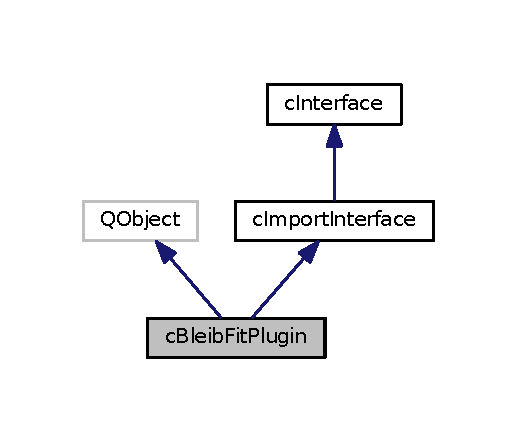
\includegraphics[width=248pt]{classc_bleib_fit_plugin__inherit__graph}
\end{center}
\end{figure}


Collaboration diagram for c\+Bleib\+Fit\+Plugin\+:
\nopagebreak
\begin{figure}[H]
\begin{center}
\leavevmode
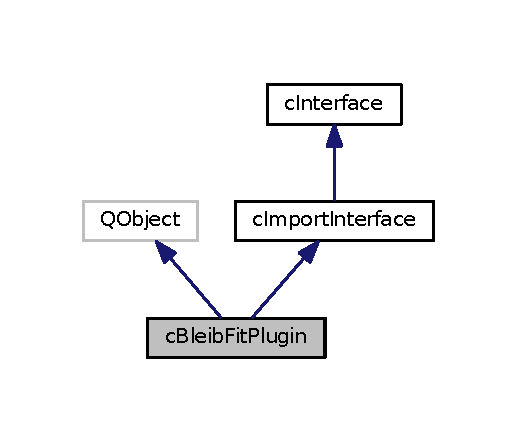
\includegraphics[width=248pt]{classc_bleib_fit_plugin__coll__graph}
\end{center}
\end{figure}
\subsection*{Public Member Functions}
\begin{DoxyCompactItemize}
\item 
qint16 \hyperlink{classc_bleib_fit_plugin_aad11be7cf80b28becc6024e3827d4f75}{plugin\+A\+P\+I\+Version} ()
\item 
Q\+String \hyperlink{classc_bleib_fit_plugin_aca281bc00f83bc4cd4b620a448825147}{plugin\+Name} ()
\item 
qint16 \hyperlink{classc_bleib_fit_plugin_acb4fbabe875079913c8bbbbe7d9089f6}{plugin\+Version} ()
\item 
\hyperlink{classc_interface_a41462a3131755963add9ba3026e7d31a}{i\+Type} \hyperlink{classc_bleib_fit_plugin_af2fc76ea7b59899780c5384721a88ebd}{plugin\+Type} ()
\item 
bool \hyperlink{classc_bleib_fit_plugin_a4ae455b66593fa29d82025b084c2639b}{config} ()
\item 
Q\+Map$<$ Q\+String, Q\+String $>$ \hyperlink{classc_bleib_fit_plugin_af3db6c6ff6bb28787d67e4cc3e957e90}{details\+Capability} ()
\item 
Q\+String\+List \hyperlink{classc_bleib_fit_plugin_a71d3dc9fc52a807e33608f2522c1ca31}{search} (const Q\+String \&sz\+Search, const Q\+String \&sz\+Details=Q\+String(\char`\"{}\char`\"{}))
\item 
bool \hyperlink{classc_bleib_fit_plugin_a15e5627fa41d2f079a96267e559fccee}{load} (qint16 i\+Index)
\item 
qreal \hyperlink{classc_bleib_fit_plugin_adb3cc6882c32a04d6d9f31961f0b8dca}{value} (\hyperlink{classc_ingredient_acf023723841ec66cd6368a25e3174a28}{c\+Ingredient\+::i\+Ingredient} i)
\item 
Q\+String \hyperlink{classc_bleib_fit_plugin_a67b808ffb0884950a8652cc72e8b2d80}{ingredient\+Name} ()
\end{DoxyCompactItemize}
\subsection*{Private Attributes}
\begin{DoxyCompactItemize}
\item 
Q\+String\+List \hyperlink{classc_bleib_fit_plugin_ada1ca6d46ebd839f6f86bfee1ed0abb8}{m\+\_\+sz\+Urls}
\item 
Q\+String\+List \hyperlink{classc_bleib_fit_plugin_a255890766758afcab2c358bfb8695a15}{m\+\_\+sz\+Ingredients}
\item 
qreal \hyperlink{classc_bleib_fit_plugin_aa9bed63f126286a26ef3b45bfa5fbdcb}{m\+\_\+r\+Values} \mbox{[}\hyperlink{classc_ingredient_acf023723841ec66cd6368a25e3174a28af55d4002286e1c85ff2fecbc7c081509}{c\+Ingredient\+::i\+Ingredient\+Max}\mbox{]}
\item 
qint16 \hyperlink{classc_bleib_fit_plugin_a381f973f2b98c90e22314a5e1855f3df}{m\+\_\+i\+Loaded\+Index}
\end{DoxyCompactItemize}
\subsection*{Additional Inherited Members}


\subsection{Member Function Documentation}
\index{c\+Bleib\+Fit\+Plugin@{c\+Bleib\+Fit\+Plugin}!config@{config}}
\index{config@{config}!c\+Bleib\+Fit\+Plugin@{c\+Bleib\+Fit\+Plugin}}
\subsubsection[{\texorpdfstring{config()}{config()}}]{\setlength{\rightskip}{0pt plus 5cm}bool c\+Bleib\+Fit\+Plugin\+::config (
\begin{DoxyParamCaption}
{}
\end{DoxyParamCaption}
)\hspace{0.3cm}{\ttfamily [virtual]}}\hypertarget{classc_bleib_fit_plugin_a4ae455b66593fa29d82025b084c2639b}{}\label{classc_bleib_fit_plugin_a4ae455b66593fa29d82025b084c2639b}
\begin{DoxyReturn}{Returns}
bool 
\end{DoxyReturn}


Implements \hyperlink{classc_interface_a040fbd069a2c2356faeda1c2d9ac88df}{c\+Interface}.



Referenced by plugin\+Type().



Here is the caller graph for this function\+:
\nopagebreak
\begin{figure}[H]
\begin{center}
\leavevmode
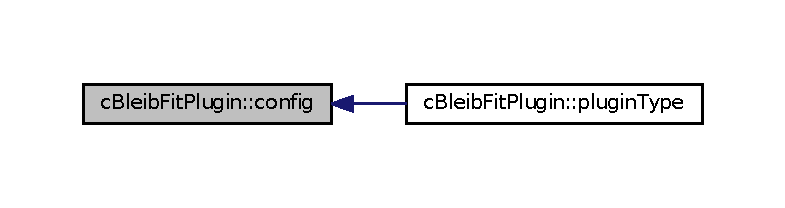
\includegraphics[width=350pt]{classc_bleib_fit_plugin_a4ae455b66593fa29d82025b084c2639b_icgraph}
\end{center}
\end{figure}


\index{c\+Bleib\+Fit\+Plugin@{c\+Bleib\+Fit\+Plugin}!details\+Capability@{details\+Capability}}
\index{details\+Capability@{details\+Capability}!c\+Bleib\+Fit\+Plugin@{c\+Bleib\+Fit\+Plugin}}
\subsubsection[{\texorpdfstring{details\+Capability()}{detailsCapability()}}]{\setlength{\rightskip}{0pt plus 5cm}Q\+Map$<$ Q\+String, Q\+String $>$ c\+Bleib\+Fit\+Plugin\+::details\+Capability (
\begin{DoxyParamCaption}
{}
\end{DoxyParamCaption}
)\hspace{0.3cm}{\ttfamily [virtual]}}\hypertarget{classc_bleib_fit_plugin_af3db6c6ff6bb28787d67e4cc3e957e90}{}\label{classc_bleib_fit_plugin_af3db6c6ff6bb28787d67e4cc3e957e90}
\begin{DoxyReturn}{Returns}
Q\+Map$<$\+Q\+String, Q\+String$>$ 
\end{DoxyReturn}


Implements \hyperlink{classc_import_interface_a4ec2f198f8488e7daf2e93cf637a580d}{c\+Import\+Interface}.



Referenced by plugin\+Type().



Here is the caller graph for this function\+:
\nopagebreak
\begin{figure}[H]
\begin{center}
\leavevmode
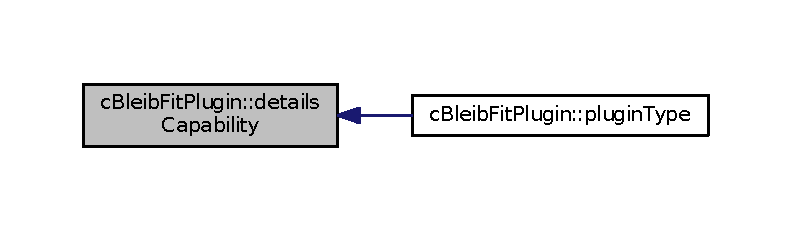
\includegraphics[width=350pt]{classc_bleib_fit_plugin_af3db6c6ff6bb28787d67e4cc3e957e90_icgraph}
\end{center}
\end{figure}


\index{c\+Bleib\+Fit\+Plugin@{c\+Bleib\+Fit\+Plugin}!ingredient\+Name@{ingredient\+Name}}
\index{ingredient\+Name@{ingredient\+Name}!c\+Bleib\+Fit\+Plugin@{c\+Bleib\+Fit\+Plugin}}
\subsubsection[{\texorpdfstring{ingredient\+Name()}{ingredientName()}}]{\setlength{\rightskip}{0pt plus 5cm}Q\+String c\+Bleib\+Fit\+Plugin\+::ingredient\+Name (
\begin{DoxyParamCaption}
{}
\end{DoxyParamCaption}
)\hspace{0.3cm}{\ttfamily [virtual]}}\hypertarget{classc_bleib_fit_plugin_a67b808ffb0884950a8652cc72e8b2d80}{}\label{classc_bleib_fit_plugin_a67b808ffb0884950a8652cc72e8b2d80}
\begin{DoxyReturn}{Returns}
Q\+String 
\end{DoxyReturn}


Implements \hyperlink{classc_import_interface_af3f569b605787021a919816978f229bc}{c\+Import\+Interface}.



Referenced by plugin\+Type().



Here is the caller graph for this function\+:
\nopagebreak
\begin{figure}[H]
\begin{center}
\leavevmode
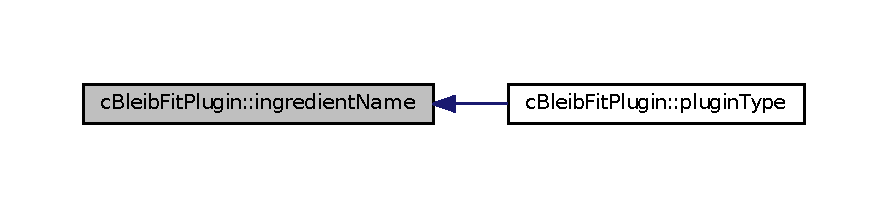
\includegraphics[width=350pt]{classc_bleib_fit_plugin_a67b808ffb0884950a8652cc72e8b2d80_icgraph}
\end{center}
\end{figure}


\index{c\+Bleib\+Fit\+Plugin@{c\+Bleib\+Fit\+Plugin}!load@{load}}
\index{load@{load}!c\+Bleib\+Fit\+Plugin@{c\+Bleib\+Fit\+Plugin}}
\subsubsection[{\texorpdfstring{load(qint16 i\+Index)}{load(qint16 iIndex)}}]{\setlength{\rightskip}{0pt plus 5cm}bool c\+Bleib\+Fit\+Plugin\+::load (
\begin{DoxyParamCaption}
\item[{qint16}]{i\+Index}
\end{DoxyParamCaption}
)\hspace{0.3cm}{\ttfamily [virtual]}}\hypertarget{classc_bleib_fit_plugin_a15e5627fa41d2f079a96267e559fccee}{}\label{classc_bleib_fit_plugin_a15e5627fa41d2f079a96267e559fccee}

\begin{DoxyParams}{Parameters}
{\em i\+Index} & \\
\hline
\end{DoxyParams}
\begin{DoxyReturn}{Returns}
bool 
\end{DoxyReturn}


Implements \hyperlink{classc_import_interface_a728bcb2a636f78bae2fe7e128a18e983}{c\+Import\+Interface}.



References tag\+M\+A\+P\+P\+E\+R\+::key, and tag\+M\+A\+P\+P\+E\+R\+::value.



Referenced by plugin\+Type().



Here is the caller graph for this function\+:
\nopagebreak
\begin{figure}[H]
\begin{center}
\leavevmode
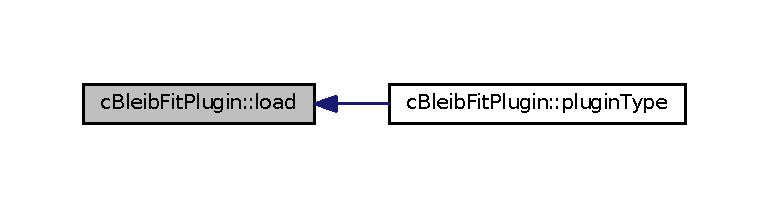
\includegraphics[width=350pt]{classc_bleib_fit_plugin_a15e5627fa41d2f079a96267e559fccee_icgraph}
\end{center}
\end{figure}


\index{c\+Bleib\+Fit\+Plugin@{c\+Bleib\+Fit\+Plugin}!plugin\+A\+P\+I\+Version@{plugin\+A\+P\+I\+Version}}
\index{plugin\+A\+P\+I\+Version@{plugin\+A\+P\+I\+Version}!c\+Bleib\+Fit\+Plugin@{c\+Bleib\+Fit\+Plugin}}
\subsubsection[{\texorpdfstring{plugin\+A\+P\+I\+Version()}{pluginAPIVersion()}}]{\setlength{\rightskip}{0pt plus 5cm}qint16 c\+Bleib\+Fit\+Plugin\+::plugin\+A\+P\+I\+Version (
\begin{DoxyParamCaption}
{}
\end{DoxyParamCaption}
)\hspace{0.3cm}{\ttfamily [inline]}, {\ttfamily [virtual]}}\hypertarget{classc_bleib_fit_plugin_aad11be7cf80b28becc6024e3827d4f75}{}\label{classc_bleib_fit_plugin_aad11be7cf80b28becc6024e3827d4f75}
\begin{DoxyReturn}{Returns}
qint16 
\end{DoxyReturn}


Implements \hyperlink{classc_interface_a615b50a526c2d4ca73b13f8991371813}{c\+Interface}.

\index{c\+Bleib\+Fit\+Plugin@{c\+Bleib\+Fit\+Plugin}!plugin\+Name@{plugin\+Name}}
\index{plugin\+Name@{plugin\+Name}!c\+Bleib\+Fit\+Plugin@{c\+Bleib\+Fit\+Plugin}}
\subsubsection[{\texorpdfstring{plugin\+Name()}{pluginName()}}]{\setlength{\rightskip}{0pt plus 5cm}Q\+String c\+Bleib\+Fit\+Plugin\+::plugin\+Name (
\begin{DoxyParamCaption}
{}
\end{DoxyParamCaption}
)\hspace{0.3cm}{\ttfamily [inline]}, {\ttfamily [virtual]}}\hypertarget{classc_bleib_fit_plugin_aca281bc00f83bc4cd4b620a448825147}{}\label{classc_bleib_fit_plugin_aca281bc00f83bc4cd4b620a448825147}
\begin{DoxyReturn}{Returns}
Q\+String 
\end{DoxyReturn}


Implements \hyperlink{classc_interface_a17e5a0cf99317ab45f624e68b4a6ecca}{c\+Interface}.

\index{c\+Bleib\+Fit\+Plugin@{c\+Bleib\+Fit\+Plugin}!plugin\+Type@{plugin\+Type}}
\index{plugin\+Type@{plugin\+Type}!c\+Bleib\+Fit\+Plugin@{c\+Bleib\+Fit\+Plugin}}
\subsubsection[{\texorpdfstring{plugin\+Type()}{pluginType()}}]{\setlength{\rightskip}{0pt plus 5cm}{\bf i\+Type} c\+Bleib\+Fit\+Plugin\+::plugin\+Type (
\begin{DoxyParamCaption}
{}
\end{DoxyParamCaption}
)\hspace{0.3cm}{\ttfamily [inline]}, {\ttfamily [virtual]}}\hypertarget{classc_bleib_fit_plugin_af2fc76ea7b59899780c5384721a88ebd}{}\label{classc_bleib_fit_plugin_af2fc76ea7b59899780c5384721a88ebd}
\begin{DoxyReturn}{Returns}
i\+Type 
\end{DoxyReturn}


Implements \hyperlink{classc_interface_af5e408cdaff527a872ce6d02a96301a4}{c\+Interface}.



References config(), details\+Capability(), ingredient\+Name(), c\+Interface\+::i\+Type\+Import, load(), search(), and value().



Here is the call graph for this function\+:
\nopagebreak
\begin{figure}[H]
\begin{center}
\leavevmode
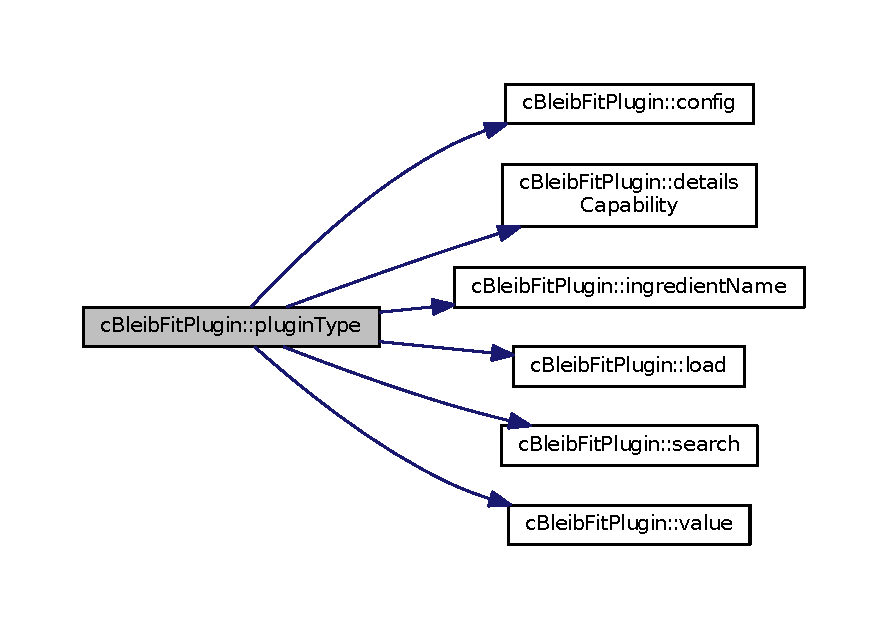
\includegraphics[width=350pt]{classc_bleib_fit_plugin_af2fc76ea7b59899780c5384721a88ebd_cgraph}
\end{center}
\end{figure}


\index{c\+Bleib\+Fit\+Plugin@{c\+Bleib\+Fit\+Plugin}!plugin\+Version@{plugin\+Version}}
\index{plugin\+Version@{plugin\+Version}!c\+Bleib\+Fit\+Plugin@{c\+Bleib\+Fit\+Plugin}}
\subsubsection[{\texorpdfstring{plugin\+Version()}{pluginVersion()}}]{\setlength{\rightskip}{0pt plus 5cm}qint16 c\+Bleib\+Fit\+Plugin\+::plugin\+Version (
\begin{DoxyParamCaption}
{}
\end{DoxyParamCaption}
)\hspace{0.3cm}{\ttfamily [inline]}, {\ttfamily [virtual]}}\hypertarget{classc_bleib_fit_plugin_acb4fbabe875079913c8bbbbe7d9089f6}{}\label{classc_bleib_fit_plugin_acb4fbabe875079913c8bbbbe7d9089f6}
\begin{DoxyReturn}{Returns}
qint16 
\end{DoxyReturn}


Implements \hyperlink{classc_interface_aadc382036174c2a25bb2c23733830d33}{c\+Interface}.

\index{c\+Bleib\+Fit\+Plugin@{c\+Bleib\+Fit\+Plugin}!search@{search}}
\index{search@{search}!c\+Bleib\+Fit\+Plugin@{c\+Bleib\+Fit\+Plugin}}
\subsubsection[{\texorpdfstring{search(const Q\+String \&sz\+Search, const Q\+String \&sz\+Details=\+Q\+String(""""))}{search(const QString &szSearch, const QString &szDetails=QString(""))}}]{\setlength{\rightskip}{0pt plus 5cm}Q\+String\+List c\+Bleib\+Fit\+Plugin\+::search (
\begin{DoxyParamCaption}
\item[{const Q\+String \&}]{sz\+Search, }
\item[{const Q\+String \&}]{sz\+Details = {\ttfamily QString(\char`\"{}\char`\"{})}}
\end{DoxyParamCaption}
)\hspace{0.3cm}{\ttfamily [virtual]}}\hypertarget{classc_bleib_fit_plugin_a71d3dc9fc52a807e33608f2522c1ca31}{}\label{classc_bleib_fit_plugin_a71d3dc9fc52a807e33608f2522c1ca31}

\begin{DoxyParams}{Parameters}
{\em sz\+Search} & \\
\hline
{\em sz\+Details} & \\
\hline
\end{DoxyParams}
\begin{DoxyReturn}{Returns}
Q\+String\+List 
\end{DoxyReturn}


Implements \hyperlink{classc_import_interface_a8b48a3821674ff15d7eaf4e03c55409f}{c\+Import\+Interface}.



References c\+Ingredient\+::i\+Ingredient\+Max.



Referenced by plugin\+Type().



Here is the caller graph for this function\+:
\nopagebreak
\begin{figure}[H]
\begin{center}
\leavevmode
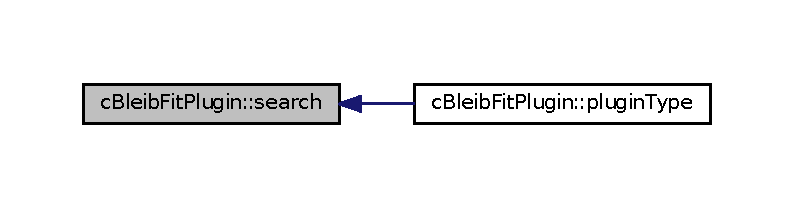
\includegraphics[width=350pt]{classc_bleib_fit_plugin_a71d3dc9fc52a807e33608f2522c1ca31_icgraph}
\end{center}
\end{figure}


\index{c\+Bleib\+Fit\+Plugin@{c\+Bleib\+Fit\+Plugin}!value@{value}}
\index{value@{value}!c\+Bleib\+Fit\+Plugin@{c\+Bleib\+Fit\+Plugin}}
\subsubsection[{\texorpdfstring{value(c\+Ingredient\+::i\+Ingredient i)}{value(cIngredient::iIngredient i)}}]{\setlength{\rightskip}{0pt plus 5cm}qreal c\+Bleib\+Fit\+Plugin\+::value (
\begin{DoxyParamCaption}
\item[{{\bf c\+Ingredient\+::i\+Ingredient}}]{i}
\end{DoxyParamCaption}
)\hspace{0.3cm}{\ttfamily [virtual]}}\hypertarget{classc_bleib_fit_plugin_adb3cc6882c32a04d6d9f31961f0b8dca}{}\label{classc_bleib_fit_plugin_adb3cc6882c32a04d6d9f31961f0b8dca}

\begin{DoxyParams}{Parameters}
{\em i} & \\
\hline
\end{DoxyParams}
\begin{DoxyReturn}{Returns}
qreal 
\end{DoxyReturn}


Implements \hyperlink{classc_import_interface_a7a8dbe6a164549272d748d2f77aebc42}{c\+Import\+Interface}.



Referenced by plugin\+Type().



Here is the caller graph for this function\+:
\nopagebreak
\begin{figure}[H]
\begin{center}
\leavevmode
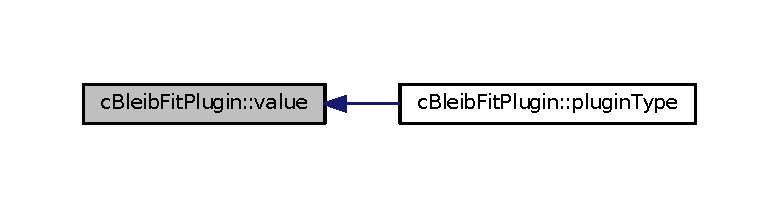
\includegraphics[width=350pt]{classc_bleib_fit_plugin_adb3cc6882c32a04d6d9f31961f0b8dca_icgraph}
\end{center}
\end{figure}




\subsection{Member Data Documentation}
\index{c\+Bleib\+Fit\+Plugin@{c\+Bleib\+Fit\+Plugin}!m\+\_\+i\+Loaded\+Index@{m\+\_\+i\+Loaded\+Index}}
\index{m\+\_\+i\+Loaded\+Index@{m\+\_\+i\+Loaded\+Index}!c\+Bleib\+Fit\+Plugin@{c\+Bleib\+Fit\+Plugin}}
\subsubsection[{\texorpdfstring{m\+\_\+i\+Loaded\+Index}{m_iLoadedIndex}}]{\setlength{\rightskip}{0pt plus 5cm}qint16 c\+Bleib\+Fit\+Plugin\+::m\+\_\+i\+Loaded\+Index\hspace{0.3cm}{\ttfamily [private]}}\hypertarget{classc_bleib_fit_plugin_a381f973f2b98c90e22314a5e1855f3df}{}\label{classc_bleib_fit_plugin_a381f973f2b98c90e22314a5e1855f3df}
T\+O\+DO\+: describe \index{c\+Bleib\+Fit\+Plugin@{c\+Bleib\+Fit\+Plugin}!m\+\_\+r\+Values@{m\+\_\+r\+Values}}
\index{m\+\_\+r\+Values@{m\+\_\+r\+Values}!c\+Bleib\+Fit\+Plugin@{c\+Bleib\+Fit\+Plugin}}
\subsubsection[{\texorpdfstring{m\+\_\+r\+Values}{m_rValues}}]{\setlength{\rightskip}{0pt plus 5cm}qreal c\+Bleib\+Fit\+Plugin\+::m\+\_\+r\+Values\mbox{[}{\bf c\+Ingredient\+::i\+Ingredient\+Max}\mbox{]}\hspace{0.3cm}{\ttfamily [private]}}\hypertarget{classc_bleib_fit_plugin_aa9bed63f126286a26ef3b45bfa5fbdcb}{}\label{classc_bleib_fit_plugin_aa9bed63f126286a26ef3b45bfa5fbdcb}
T\+O\+DO\+: describe \index{c\+Bleib\+Fit\+Plugin@{c\+Bleib\+Fit\+Plugin}!m\+\_\+sz\+Ingredients@{m\+\_\+sz\+Ingredients}}
\index{m\+\_\+sz\+Ingredients@{m\+\_\+sz\+Ingredients}!c\+Bleib\+Fit\+Plugin@{c\+Bleib\+Fit\+Plugin}}
\subsubsection[{\texorpdfstring{m\+\_\+sz\+Ingredients}{m_szIngredients}}]{\setlength{\rightskip}{0pt plus 5cm}Q\+String\+List c\+Bleib\+Fit\+Plugin\+::m\+\_\+sz\+Ingredients\hspace{0.3cm}{\ttfamily [private]}}\hypertarget{classc_bleib_fit_plugin_a255890766758afcab2c358bfb8695a15}{}\label{classc_bleib_fit_plugin_a255890766758afcab2c358bfb8695a15}
T\+O\+DO\+: describe \index{c\+Bleib\+Fit\+Plugin@{c\+Bleib\+Fit\+Plugin}!m\+\_\+sz\+Urls@{m\+\_\+sz\+Urls}}
\index{m\+\_\+sz\+Urls@{m\+\_\+sz\+Urls}!c\+Bleib\+Fit\+Plugin@{c\+Bleib\+Fit\+Plugin}}
\subsubsection[{\texorpdfstring{m\+\_\+sz\+Urls}{m_szUrls}}]{\setlength{\rightskip}{0pt plus 5cm}Q\+String\+List c\+Bleib\+Fit\+Plugin\+::m\+\_\+sz\+Urls\hspace{0.3cm}{\ttfamily [private]}}\hypertarget{classc_bleib_fit_plugin_ada1ca6d46ebd839f6f86bfee1ed0abb8}{}\label{classc_bleib_fit_plugin_ada1ca6d46ebd839f6f86bfee1ed0abb8}
T\+O\+DO\+: describe 

The documentation for this class was generated from the following files\+:\begin{DoxyCompactItemize}
\item 
i\+Bleib\+Fit/\hyperlink{cbleibfitplugin_8h}{cbleibfitplugin.\+h}\item 
i\+Bleib\+Fit/\hyperlink{cbleibfitplugin_8cpp}{cbleibfitplugin.\+cpp}\end{DoxyCompactItemize}

\hypertarget{classc_config_dialog}{}\section{c\+Config\+Dialog Class Reference}
\label{classc_config_dialog}\index{c\+Config\+Dialog@{c\+Config\+Dialog}}


Configuration Dialog for d\+My\+S\+QL.  




{\ttfamily \#include $<$cconfigdialog.\+h$>$}



Inheritance diagram for c\+Config\+Dialog\+:
\nopagebreak
\begin{figure}[H]
\begin{center}
\leavevmode
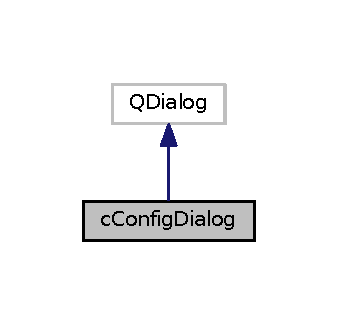
\includegraphics[width=162pt]{classc_config_dialog__inherit__graph}
\end{center}
\end{figure}


Collaboration diagram for c\+Config\+Dialog\+:
\nopagebreak
\begin{figure}[H]
\begin{center}
\leavevmode
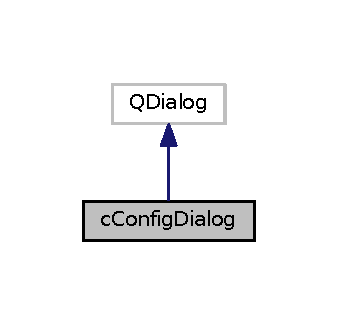
\includegraphics[width=162pt]{classc_config_dialog__coll__graph}
\end{center}
\end{figure}
\subsection*{Public Member Functions}
\begin{DoxyCompactItemize}
\item 
\hyperlink{classc_config_dialog_aa89869d702a4d9a2dd94086bc8d700ee}{c\+Config\+Dialog} (Q\+Widget $\ast$parent=0)
\item 
\hyperlink{classc_config_dialog_ae88187dcf8dfc433b53b26bd5e54f871}{$\sim$c\+Config\+Dialog} ()
\item 
void \hyperlink{classc_config_dialog_acb0a82e1653578edc43855af17154f24}{set\+Hostname} (const Q\+String \&sz\+Hostname)
\item 
void \hyperlink{classc_config_dialog_abcb15989a34c945128e8624b93b5c272}{set\+Database} (const Q\+String \&sz\+Database)
\item 
void \hyperlink{classc_config_dialog_ae3238bbd8055b58066046840fef448b4}{set\+User\+Name} (const Q\+String \&sz\+User\+Name)
\item 
void \hyperlink{classc_config_dialog_a1eecd4be7061043a3ae60473013edfb1}{set\+Password} (const Q\+String \&sz\+Password)
\item 
Q\+String \hyperlink{classc_config_dialog_a77e56b372e8914cf531d64054cbaea2c}{hostname} ()
\item 
Q\+String \hyperlink{classc_config_dialog_a1ab3c4cf07b4bb84624ddfe4395a1935}{database} ()
\item 
Q\+String \hyperlink{classc_config_dialog_ad1f4eda37fec241ffbcc158c039accea}{user\+Name} ()
\item 
Q\+String \hyperlink{classc_config_dialog_aea1dfbe7eae14e7949a15631ed2df8a5}{password} ()
\end{DoxyCompactItemize}
\subsection*{Private Slots}
\begin{DoxyCompactItemize}
\item 
void \hyperlink{classc_config_dialog_a7fb2127745f898b2c7fd8306ea7df149}{on\+\_\+m\+\_\+lp\+Test\+Button\+\_\+clicked} ()
\item 
void \hyperlink{classc_config_dialog_a06a5e35e33fe97b46813ecb70fddb1ef}{on\+\_\+m\+\_\+lp\+Password\+\_\+text\+Changed} (const Q\+String \&arg1)
\item 
void \hyperlink{classc_config_dialog_aaf2c308f17983e14ac6ea8824ffa99c4}{on\+\_\+m\+\_\+lp\+Password2\+\_\+text\+Changed} (const Q\+String \&arg1)
\item 
void \hyperlink{classc_config_dialog_ab1dd081ac31a02ff0d53d2f271fdeed5}{on\+\_\+m\+\_\+lp\+O\+K\+Button\+\_\+clicked} ()
\item 
void \hyperlink{classc_config_dialog_ac70b6c699e0eb5af4397a5a2ff29789a}{on\+\_\+m\+\_\+lp\+Cancel\+Button\+\_\+clicked} ()
\end{DoxyCompactItemize}
\subsection*{Private Attributes}
\begin{DoxyCompactItemize}
\item 
Ui\+::c\+Config\+Dialog $\ast$ \hyperlink{classc_config_dialog_a57a160e7fe62e54d86b7f3592aaee2f6}{ui}
\item 
bool \hyperlink{classc_config_dialog_a68daa09e2f01b7f7108b5d91fcd32df1}{m\+\_\+b\+Password\+Changed}
\end{DoxyCompactItemize}


\subsection{Detailed Description}
This class implements basic import functionality for Kooky. All functions may be overwritten by derriving classes.

\begin{DoxyNote}{Note}
Attempts at zen rarely work.
\end{DoxyNote}
\begin{DoxyAuthor}{Author}
Herwig Birke
\end{DoxyAuthor}
\begin{DoxyVersion}{Version}
1.\+0
\end{DoxyVersion}
\begin{DoxyDate}{Date}
2016/02/09 
\end{DoxyDate}


\subsection{Constructor \& Destructor Documentation}
\index{c\+Config\+Dialog@{c\+Config\+Dialog}!c\+Config\+Dialog@{c\+Config\+Dialog}}
\index{c\+Config\+Dialog@{c\+Config\+Dialog}!c\+Config\+Dialog@{c\+Config\+Dialog}}
\subsubsection[{\texorpdfstring{c\+Config\+Dialog(\+Q\+Widget $\ast$parent=0)}{cConfigDialog(QWidget *parent=0)}}]{\setlength{\rightskip}{0pt plus 5cm}c\+Config\+Dialog\+::c\+Config\+Dialog (
\begin{DoxyParamCaption}
\item[{Q\+Widget $\ast$}]{parent = {\ttfamily 0}}
\end{DoxyParamCaption}
)\hspace{0.3cm}{\ttfamily [explicit]}}\hypertarget{classc_config_dialog_aa89869d702a4d9a2dd94086bc8d700ee}{}\label{classc_config_dialog_aa89869d702a4d9a2dd94086bc8d700ee}

\begin{DoxyParams}{Parameters}
{\em parent} & \\
\hline
\end{DoxyParams}


References ui.

\index{c\+Config\+Dialog@{c\+Config\+Dialog}!````~c\+Config\+Dialog@{$\sim$c\+Config\+Dialog}}
\index{````~c\+Config\+Dialog@{$\sim$c\+Config\+Dialog}!c\+Config\+Dialog@{c\+Config\+Dialog}}
\subsubsection[{\texorpdfstring{$\sim$c\+Config\+Dialog()}{~cConfigDialog()}}]{\setlength{\rightskip}{0pt plus 5cm}c\+Config\+Dialog\+::$\sim$c\+Config\+Dialog (
\begin{DoxyParamCaption}
{}
\end{DoxyParamCaption}
)}\hypertarget{classc_config_dialog_ae88187dcf8dfc433b53b26bd5e54f871}{}\label{classc_config_dialog_ae88187dcf8dfc433b53b26bd5e54f871}


References ui.



\subsection{Member Function Documentation}
\index{c\+Config\+Dialog@{c\+Config\+Dialog}!database@{database}}
\index{database@{database}!c\+Config\+Dialog@{c\+Config\+Dialog}}
\subsubsection[{\texorpdfstring{database()}{database()}}]{\setlength{\rightskip}{0pt plus 5cm}Q\+String c\+Config\+Dialog\+::database (
\begin{DoxyParamCaption}
{}
\end{DoxyParamCaption}
)}\hypertarget{classc_config_dialog_a1ab3c4cf07b4bb84624ddfe4395a1935}{}\label{classc_config_dialog_a1ab3c4cf07b4bb84624ddfe4395a1935}
\begin{DoxyReturn}{Returns}
Q\+String 
\end{DoxyReturn}


References ui.



Referenced by c\+My\+S\+Q\+L\+Plugin\+::config().



Here is the caller graph for this function\+:
\nopagebreak
\begin{figure}[H]
\begin{center}
\leavevmode
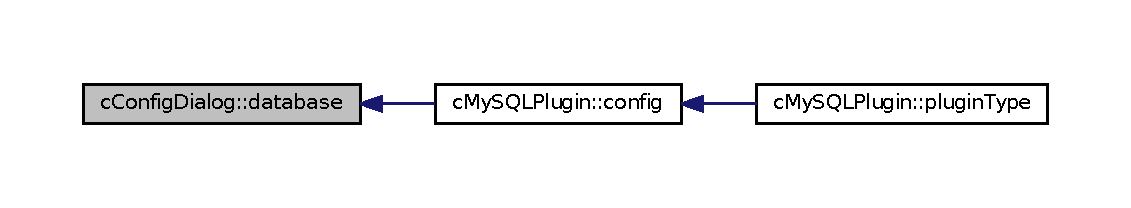
\includegraphics[width=350pt]{classc_config_dialog_a1ab3c4cf07b4bb84624ddfe4395a1935_icgraph}
\end{center}
\end{figure}


\index{c\+Config\+Dialog@{c\+Config\+Dialog}!hostname@{hostname}}
\index{hostname@{hostname}!c\+Config\+Dialog@{c\+Config\+Dialog}}
\subsubsection[{\texorpdfstring{hostname()}{hostname()}}]{\setlength{\rightskip}{0pt plus 5cm}Q\+String c\+Config\+Dialog\+::hostname (
\begin{DoxyParamCaption}
{}
\end{DoxyParamCaption}
)}\hypertarget{classc_config_dialog_a77e56b372e8914cf531d64054cbaea2c}{}\label{classc_config_dialog_a77e56b372e8914cf531d64054cbaea2c}
\begin{DoxyReturn}{Returns}
Q\+String 
\end{DoxyReturn}


References ui.



Referenced by c\+My\+S\+Q\+L\+Plugin\+::config().



Here is the caller graph for this function\+:
\nopagebreak
\begin{figure}[H]
\begin{center}
\leavevmode
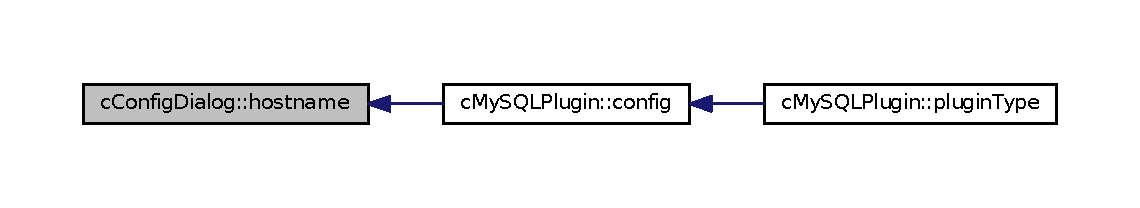
\includegraphics[width=350pt]{classc_config_dialog_a77e56b372e8914cf531d64054cbaea2c_icgraph}
\end{center}
\end{figure}


\index{c\+Config\+Dialog@{c\+Config\+Dialog}!on\+\_\+m\+\_\+lp\+Cancel\+Button\+\_\+clicked@{on\+\_\+m\+\_\+lp\+Cancel\+Button\+\_\+clicked}}
\index{on\+\_\+m\+\_\+lp\+Cancel\+Button\+\_\+clicked@{on\+\_\+m\+\_\+lp\+Cancel\+Button\+\_\+clicked}!c\+Config\+Dialog@{c\+Config\+Dialog}}
\subsubsection[{\texorpdfstring{on\+\_\+m\+\_\+lp\+Cancel\+Button\+\_\+clicked}{on_m_lpCancelButton_clicked}}]{\setlength{\rightskip}{0pt plus 5cm}void c\+Config\+Dialog\+::on\+\_\+m\+\_\+lp\+Cancel\+Button\+\_\+clicked (
\begin{DoxyParamCaption}
{}
\end{DoxyParamCaption}
)\hspace{0.3cm}{\ttfamily [private]}, {\ttfamily [slot]}}\hypertarget{classc_config_dialog_ac70b6c699e0eb5af4397a5a2ff29789a}{}\label{classc_config_dialog_ac70b6c699e0eb5af4397a5a2ff29789a}
\index{c\+Config\+Dialog@{c\+Config\+Dialog}!on\+\_\+m\+\_\+lp\+O\+K\+Button\+\_\+clicked@{on\+\_\+m\+\_\+lp\+O\+K\+Button\+\_\+clicked}}
\index{on\+\_\+m\+\_\+lp\+O\+K\+Button\+\_\+clicked@{on\+\_\+m\+\_\+lp\+O\+K\+Button\+\_\+clicked}!c\+Config\+Dialog@{c\+Config\+Dialog}}
\subsubsection[{\texorpdfstring{on\+\_\+m\+\_\+lp\+O\+K\+Button\+\_\+clicked}{on_m_lpOKButton_clicked}}]{\setlength{\rightskip}{0pt plus 5cm}void c\+Config\+Dialog\+::on\+\_\+m\+\_\+lp\+O\+K\+Button\+\_\+clicked (
\begin{DoxyParamCaption}
{}
\end{DoxyParamCaption}
)\hspace{0.3cm}{\ttfamily [private]}, {\ttfamily [slot]}}\hypertarget{classc_config_dialog_ab1dd081ac31a02ff0d53d2f271fdeed5}{}\label{classc_config_dialog_ab1dd081ac31a02ff0d53d2f271fdeed5}


References ui.

\index{c\+Config\+Dialog@{c\+Config\+Dialog}!on\+\_\+m\+\_\+lp\+Password2\+\_\+text\+Changed@{on\+\_\+m\+\_\+lp\+Password2\+\_\+text\+Changed}}
\index{on\+\_\+m\+\_\+lp\+Password2\+\_\+text\+Changed@{on\+\_\+m\+\_\+lp\+Password2\+\_\+text\+Changed}!c\+Config\+Dialog@{c\+Config\+Dialog}}
\subsubsection[{\texorpdfstring{on\+\_\+m\+\_\+lp\+Password2\+\_\+text\+Changed}{on_m_lpPassword2_textChanged}}]{\setlength{\rightskip}{0pt plus 5cm}void c\+Config\+Dialog\+::on\+\_\+m\+\_\+lp\+Password2\+\_\+text\+Changed (
\begin{DoxyParamCaption}
\item[{const Q\+String \&}]{arg1}
\end{DoxyParamCaption}
)\hspace{0.3cm}{\ttfamily [private]}, {\ttfamily [slot]}}\hypertarget{classc_config_dialog_aaf2c308f17983e14ac6ea8824ffa99c4}{}\label{classc_config_dialog_aaf2c308f17983e14ac6ea8824ffa99c4}

\begin{DoxyParams}{Parameters}
{\em arg1} & \\
\hline
\end{DoxyParams}


References m\+\_\+b\+Password\+Changed, and ui.

\index{c\+Config\+Dialog@{c\+Config\+Dialog}!on\+\_\+m\+\_\+lp\+Password\+\_\+text\+Changed@{on\+\_\+m\+\_\+lp\+Password\+\_\+text\+Changed}}
\index{on\+\_\+m\+\_\+lp\+Password\+\_\+text\+Changed@{on\+\_\+m\+\_\+lp\+Password\+\_\+text\+Changed}!c\+Config\+Dialog@{c\+Config\+Dialog}}
\subsubsection[{\texorpdfstring{on\+\_\+m\+\_\+lp\+Password\+\_\+text\+Changed}{on_m_lpPassword_textChanged}}]{\setlength{\rightskip}{0pt plus 5cm}void c\+Config\+Dialog\+::on\+\_\+m\+\_\+lp\+Password\+\_\+text\+Changed (
\begin{DoxyParamCaption}
\item[{const Q\+String \&}]{arg1}
\end{DoxyParamCaption}
)\hspace{0.3cm}{\ttfamily [private]}, {\ttfamily [slot]}}\hypertarget{classc_config_dialog_a06a5e35e33fe97b46813ecb70fddb1ef}{}\label{classc_config_dialog_a06a5e35e33fe97b46813ecb70fddb1ef}

\begin{DoxyParams}{Parameters}
{\em arg1} & \\
\hline
\end{DoxyParams}


References m\+\_\+b\+Password\+Changed, and ui.

\index{c\+Config\+Dialog@{c\+Config\+Dialog}!on\+\_\+m\+\_\+lp\+Test\+Button\+\_\+clicked@{on\+\_\+m\+\_\+lp\+Test\+Button\+\_\+clicked}}
\index{on\+\_\+m\+\_\+lp\+Test\+Button\+\_\+clicked@{on\+\_\+m\+\_\+lp\+Test\+Button\+\_\+clicked}!c\+Config\+Dialog@{c\+Config\+Dialog}}
\subsubsection[{\texorpdfstring{on\+\_\+m\+\_\+lp\+Test\+Button\+\_\+clicked}{on_m_lpTestButton_clicked}}]{\setlength{\rightskip}{0pt plus 5cm}void c\+Config\+Dialog\+::on\+\_\+m\+\_\+lp\+Test\+Button\+\_\+clicked (
\begin{DoxyParamCaption}
{}
\end{DoxyParamCaption}
)\hspace{0.3cm}{\ttfamily [private]}, {\ttfamily [slot]}}\hypertarget{classc_config_dialog_a7fb2127745f898b2c7fd8306ea7df149}{}\label{classc_config_dialog_a7fb2127745f898b2c7fd8306ea7df149}
\index{c\+Config\+Dialog@{c\+Config\+Dialog}!password@{password}}
\index{password@{password}!c\+Config\+Dialog@{c\+Config\+Dialog}}
\subsubsection[{\texorpdfstring{password()}{password()}}]{\setlength{\rightskip}{0pt plus 5cm}Q\+String c\+Config\+Dialog\+::password (
\begin{DoxyParamCaption}
{}
\end{DoxyParamCaption}
)}\hypertarget{classc_config_dialog_aea1dfbe7eae14e7949a15631ed2df8a5}{}\label{classc_config_dialog_aea1dfbe7eae14e7949a15631ed2df8a5}
\begin{DoxyReturn}{Returns}
Q\+String 
\end{DoxyReturn}


References ui.



Referenced by c\+My\+S\+Q\+L\+Plugin\+::config().



Here is the caller graph for this function\+:
\nopagebreak
\begin{figure}[H]
\begin{center}
\leavevmode
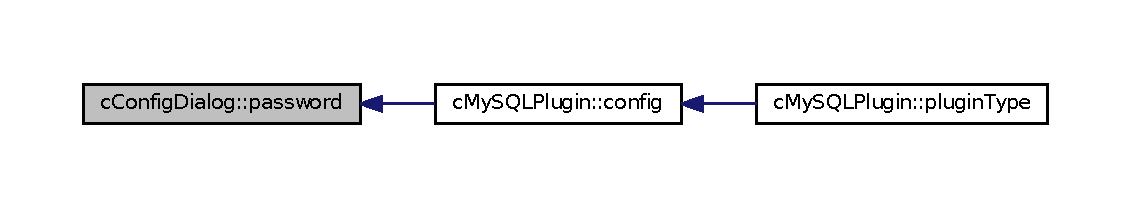
\includegraphics[width=350pt]{classc_config_dialog_aea1dfbe7eae14e7949a15631ed2df8a5_icgraph}
\end{center}
\end{figure}


\index{c\+Config\+Dialog@{c\+Config\+Dialog}!set\+Database@{set\+Database}}
\index{set\+Database@{set\+Database}!c\+Config\+Dialog@{c\+Config\+Dialog}}
\subsubsection[{\texorpdfstring{set\+Database(const Q\+String \&sz\+Database)}{setDatabase(const QString &szDatabase)}}]{\setlength{\rightskip}{0pt plus 5cm}void c\+Config\+Dialog\+::set\+Database (
\begin{DoxyParamCaption}
\item[{const Q\+String \&}]{sz\+Database}
\end{DoxyParamCaption}
)}\hypertarget{classc_config_dialog_abcb15989a34c945128e8624b93b5c272}{}\label{classc_config_dialog_abcb15989a34c945128e8624b93b5c272}

\begin{DoxyParams}{Parameters}
{\em sz\+Database} & \\
\hline
\end{DoxyParams}


References ui.



Referenced by c\+My\+S\+Q\+L\+Plugin\+::config().



Here is the caller graph for this function\+:
\nopagebreak
\begin{figure}[H]
\begin{center}
\leavevmode
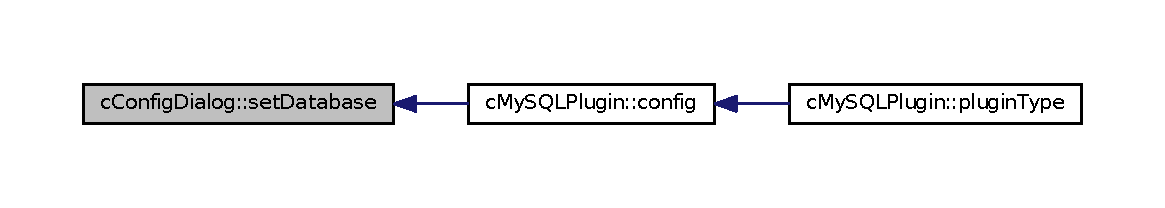
\includegraphics[width=350pt]{classc_config_dialog_abcb15989a34c945128e8624b93b5c272_icgraph}
\end{center}
\end{figure}


\index{c\+Config\+Dialog@{c\+Config\+Dialog}!set\+Hostname@{set\+Hostname}}
\index{set\+Hostname@{set\+Hostname}!c\+Config\+Dialog@{c\+Config\+Dialog}}
\subsubsection[{\texorpdfstring{set\+Hostname(const Q\+String \&sz\+Hostname)}{setHostname(const QString &szHostname)}}]{\setlength{\rightskip}{0pt plus 5cm}void c\+Config\+Dialog\+::set\+Hostname (
\begin{DoxyParamCaption}
\item[{const Q\+String \&}]{sz\+Hostname}
\end{DoxyParamCaption}
)}\hypertarget{classc_config_dialog_acb0a82e1653578edc43855af17154f24}{}\label{classc_config_dialog_acb0a82e1653578edc43855af17154f24}

\begin{DoxyParams}{Parameters}
{\em sz\+Hostname} & \\
\hline
\end{DoxyParams}


References ui.



Referenced by c\+My\+S\+Q\+L\+Plugin\+::config().



Here is the caller graph for this function\+:
\nopagebreak
\begin{figure}[H]
\begin{center}
\leavevmode
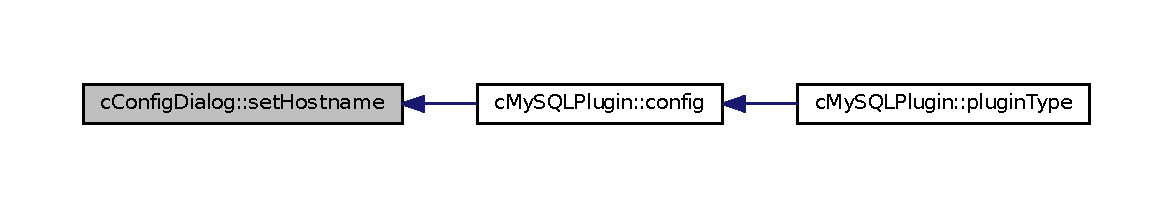
\includegraphics[width=350pt]{classc_config_dialog_acb0a82e1653578edc43855af17154f24_icgraph}
\end{center}
\end{figure}


\index{c\+Config\+Dialog@{c\+Config\+Dialog}!set\+Password@{set\+Password}}
\index{set\+Password@{set\+Password}!c\+Config\+Dialog@{c\+Config\+Dialog}}
\subsubsection[{\texorpdfstring{set\+Password(const Q\+String \&sz\+Password)}{setPassword(const QString &szPassword)}}]{\setlength{\rightskip}{0pt plus 5cm}void c\+Config\+Dialog\+::set\+Password (
\begin{DoxyParamCaption}
\item[{const Q\+String \&}]{sz\+Password}
\end{DoxyParamCaption}
)}\hypertarget{classc_config_dialog_a1eecd4be7061043a3ae60473013edfb1}{}\label{classc_config_dialog_a1eecd4be7061043a3ae60473013edfb1}

\begin{DoxyParams}{Parameters}
{\em sz\+Password} & \\
\hline
\end{DoxyParams}


References ui.



Referenced by c\+My\+S\+Q\+L\+Plugin\+::config().



Here is the caller graph for this function\+:
\nopagebreak
\begin{figure}[H]
\begin{center}
\leavevmode
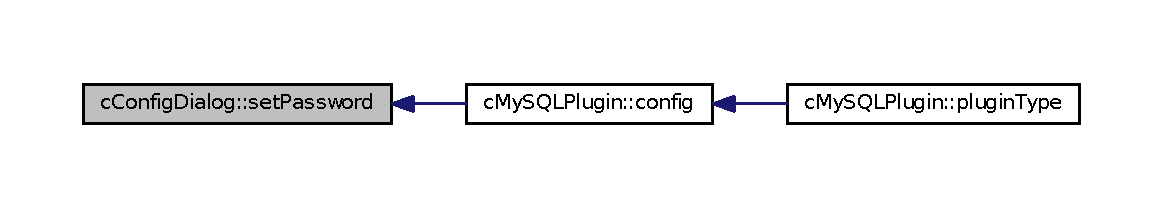
\includegraphics[width=350pt]{classc_config_dialog_a1eecd4be7061043a3ae60473013edfb1_icgraph}
\end{center}
\end{figure}


\index{c\+Config\+Dialog@{c\+Config\+Dialog}!set\+User\+Name@{set\+User\+Name}}
\index{set\+User\+Name@{set\+User\+Name}!c\+Config\+Dialog@{c\+Config\+Dialog}}
\subsubsection[{\texorpdfstring{set\+User\+Name(const Q\+String \&sz\+User\+Name)}{setUserName(const QString &szUserName)}}]{\setlength{\rightskip}{0pt plus 5cm}void c\+Config\+Dialog\+::set\+User\+Name (
\begin{DoxyParamCaption}
\item[{const Q\+String \&}]{sz\+User\+Name}
\end{DoxyParamCaption}
)}\hypertarget{classc_config_dialog_ae3238bbd8055b58066046840fef448b4}{}\label{classc_config_dialog_ae3238bbd8055b58066046840fef448b4}

\begin{DoxyParams}{Parameters}
{\em sz\+User\+Name} & \\
\hline
\end{DoxyParams}


References ui.



Referenced by c\+My\+S\+Q\+L\+Plugin\+::config().



Here is the caller graph for this function\+:
\nopagebreak
\begin{figure}[H]
\begin{center}
\leavevmode
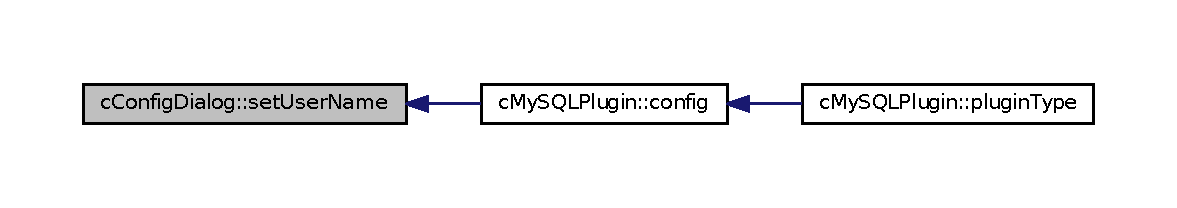
\includegraphics[width=350pt]{classc_config_dialog_ae3238bbd8055b58066046840fef448b4_icgraph}
\end{center}
\end{figure}


\index{c\+Config\+Dialog@{c\+Config\+Dialog}!user\+Name@{user\+Name}}
\index{user\+Name@{user\+Name}!c\+Config\+Dialog@{c\+Config\+Dialog}}
\subsubsection[{\texorpdfstring{user\+Name()}{userName()}}]{\setlength{\rightskip}{0pt plus 5cm}Q\+String c\+Config\+Dialog\+::user\+Name (
\begin{DoxyParamCaption}
{}
\end{DoxyParamCaption}
)}\hypertarget{classc_config_dialog_ad1f4eda37fec241ffbcc158c039accea}{}\label{classc_config_dialog_ad1f4eda37fec241ffbcc158c039accea}
\begin{DoxyReturn}{Returns}
Q\+String 
\end{DoxyReturn}


References ui.



Referenced by c\+My\+S\+Q\+L\+Plugin\+::config().



Here is the caller graph for this function\+:
\nopagebreak
\begin{figure}[H]
\begin{center}
\leavevmode
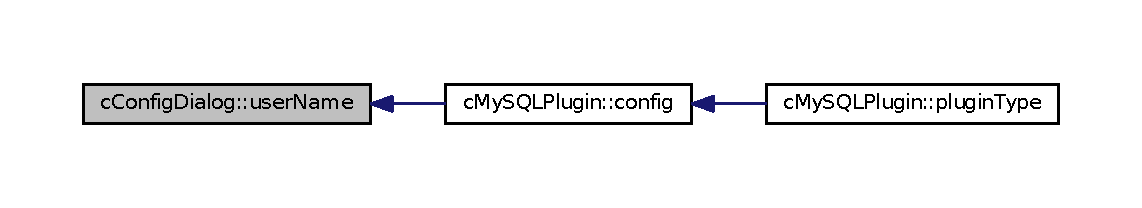
\includegraphics[width=350pt]{classc_config_dialog_ad1f4eda37fec241ffbcc158c039accea_icgraph}
\end{center}
\end{figure}




\subsection{Member Data Documentation}
\index{c\+Config\+Dialog@{c\+Config\+Dialog}!m\+\_\+b\+Password\+Changed@{m\+\_\+b\+Password\+Changed}}
\index{m\+\_\+b\+Password\+Changed@{m\+\_\+b\+Password\+Changed}!c\+Config\+Dialog@{c\+Config\+Dialog}}
\subsubsection[{\texorpdfstring{m\+\_\+b\+Password\+Changed}{m_bPasswordChanged}}]{\setlength{\rightskip}{0pt plus 5cm}bool c\+Config\+Dialog\+::m\+\_\+b\+Password\+Changed\hspace{0.3cm}{\ttfamily [private]}}\hypertarget{classc_config_dialog_a68daa09e2f01b7f7108b5d91fcd32df1}{}\label{classc_config_dialog_a68daa09e2f01b7f7108b5d91fcd32df1}
T\+O\+DO\+: describe 

Referenced by on\+\_\+m\+\_\+lp\+Password2\+\_\+text\+Changed(), and on\+\_\+m\+\_\+lp\+Password\+\_\+text\+Changed().

\index{c\+Config\+Dialog@{c\+Config\+Dialog}!ui@{ui}}
\index{ui@{ui}!c\+Config\+Dialog@{c\+Config\+Dialog}}
\subsubsection[{\texorpdfstring{ui}{ui}}]{\setlength{\rightskip}{0pt plus 5cm}Ui\+::c\+Config\+Dialog$\ast$ c\+Config\+Dialog\+::ui\hspace{0.3cm}{\ttfamily [private]}}\hypertarget{classc_config_dialog_a57a160e7fe62e54d86b7f3592aaee2f6}{}\label{classc_config_dialog_a57a160e7fe62e54d86b7f3592aaee2f6}
T\+O\+DO\+: describe 

Referenced by c\+Config\+Dialog(), database(), hostname(), on\+\_\+m\+\_\+lp\+O\+K\+Button\+\_\+clicked(), on\+\_\+m\+\_\+lp\+Password2\+\_\+text\+Changed(), on\+\_\+m\+\_\+lp\+Password\+\_\+text\+Changed(), password(), set\+Database(), set\+Hostname(), set\+Password(), set\+User\+Name(), user\+Name(), and $\sim$c\+Config\+Dialog().



The documentation for this class was generated from the following files\+:\begin{DoxyCompactItemize}
\item 
d\+My\+S\+Q\+L/\hyperlink{cconfigdialog_8h}{cconfigdialog.\+h}\item 
d\+My\+S\+Q\+L/\hyperlink{cconfigdialog_8cpp}{cconfigdialog.\+cpp}\end{DoxyCompactItemize}

\hypertarget{classc_d_b_interface}{}\section{c\+D\+B\+Interface Class Reference}
\label{classc_d_b_interface}\index{c\+D\+B\+Interface@{c\+D\+B\+Interface}}


This is the base class for all database connector plugins.  




{\ttfamily \#include $<$cdbinterface.\+h$>$}



Inheritance diagram for c\+D\+B\+Interface\+:
\nopagebreak
\begin{figure}[H]
\begin{center}
\leavevmode
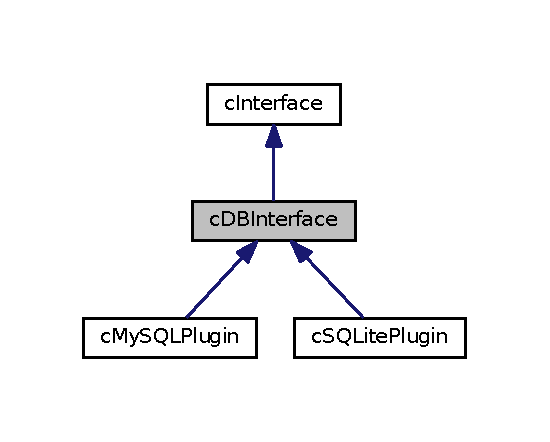
\includegraphics[width=264pt]{classc_d_b_interface__inherit__graph}
\end{center}
\end{figure}


Collaboration diagram for c\+D\+B\+Interface\+:
\nopagebreak
\begin{figure}[H]
\begin{center}
\leavevmode
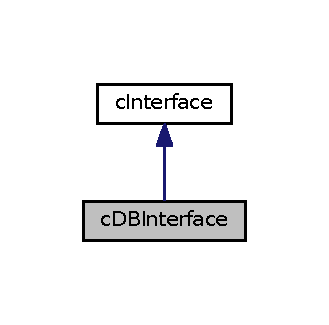
\includegraphics[width=158pt]{classc_d_b_interface__coll__graph}
\end{center}
\end{figure}
\subsection*{Public Member Functions}
\begin{DoxyCompactItemize}
\item 
\hyperlink{classc_d_b_interface_a71fd9c721e72a05983a061ba8348f257}{c\+D\+B\+Interface} ()
\begin{DoxyCompactList}\small\item\em Constructor. \end{DoxyCompactList}\item 
virtual \hyperlink{classc_d_b_interface_a7146e4fb1753d18c5f13908505fb8b4c}{$\sim$c\+D\+B\+Interface} ()
\begin{DoxyCompactList}\small\item\em Destructor. \end{DoxyCompactList}\item 
virtual bool \hyperlink{classc_d_b_interface_a1831bb8f93342190f26d83f35b4a988b}{connect} ()=0
\begin{DoxyCompactList}\small\item\em Opens a connection to the database. \end{DoxyCompactList}\item 
virtual bool \hyperlink{classc_d_b_interface_a8baa6f378fb91dea077b38bd15be12c9}{init} ()=0
\begin{DoxyCompactList}\small\item\em Initializes the module with default values. \end{DoxyCompactList}\item 
bool \hyperlink{classc_d_b_interface_a31ca3accfbd6dd1d2915440a94874b7b}{connected} ()
\begin{DoxyCompactList}\small\item\em Returns the current connection status. \end{DoxyCompactList}\item 
Q\+String \hyperlink{classc_d_b_interface_a280fe85549741179ce3a23b9f417c689}{last\+Error} ()
\begin{DoxyCompactList}\small\item\em Returns the last error message of the last operation. \end{DoxyCompactList}\end{DoxyCompactItemize}
\subsection*{Protected Attributes}
\begin{DoxyCompactItemize}
\item 
bool \hyperlink{classc_d_b_interface_a28d4d17206ee596e43e8c433c11c9282}{m\+\_\+b\+Connected}
\end{DoxyCompactItemize}
\subsection*{Additional Inherited Members}


\subsection{Detailed Description}
This class implements basic interface functionality for all Kooky database connector plugins. All functions may be overwritten by derriving classes.

\begin{DoxyNote}{Note}

\end{DoxyNote}
\begin{DoxyAuthor}{Author}
Herwig Birke
\end{DoxyAuthor}
\begin{DoxyVersion}{Version}
1.\+0
\end{DoxyVersion}
\begin{DoxyDate}{Date}
2016/02/09 
\end{DoxyDate}


\subsection{Constructor \& Destructor Documentation}
\index{c\+D\+B\+Interface@{c\+D\+B\+Interface}!c\+D\+B\+Interface@{c\+D\+B\+Interface}}
\index{c\+D\+B\+Interface@{c\+D\+B\+Interface}!c\+D\+B\+Interface@{c\+D\+B\+Interface}}
\subsubsection[{\texorpdfstring{c\+D\+B\+Interface()}{cDBInterface()}}]{\setlength{\rightskip}{0pt plus 5cm}c\+D\+B\+Interface\+::c\+D\+B\+Interface (
\begin{DoxyParamCaption}
{}
\end{DoxyParamCaption}
)\hspace{0.3cm}{\ttfamily [inline]}}\hypertarget{classc_d_b_interface_a71fd9c721e72a05983a061ba8348f257}{}\label{classc_d_b_interface_a71fd9c721e72a05983a061ba8348f257}
\index{c\+D\+B\+Interface@{c\+D\+B\+Interface}!````~c\+D\+B\+Interface@{$\sim$c\+D\+B\+Interface}}
\index{````~c\+D\+B\+Interface@{$\sim$c\+D\+B\+Interface}!c\+D\+B\+Interface@{c\+D\+B\+Interface}}
\subsubsection[{\texorpdfstring{$\sim$c\+D\+B\+Interface()}{~cDBInterface()}}]{\setlength{\rightskip}{0pt plus 5cm}virtual c\+D\+B\+Interface\+::$\sim$c\+D\+B\+Interface (
\begin{DoxyParamCaption}
{}
\end{DoxyParamCaption}
)\hspace{0.3cm}{\ttfamily [inline]}, {\ttfamily [virtual]}}\hypertarget{classc_d_b_interface_a7146e4fb1753d18c5f13908505fb8b4c}{}\label{classc_d_b_interface_a7146e4fb1753d18c5f13908505fb8b4c}


References connect(), and init().



Here is the call graph for this function\+:
\nopagebreak
\begin{figure}[H]
\begin{center}
\leavevmode
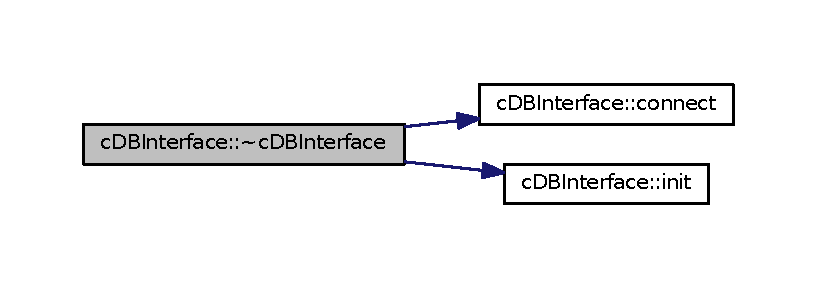
\includegraphics[width=350pt]{classc_d_b_interface_a7146e4fb1753d18c5f13908505fb8b4c_cgraph}
\end{center}
\end{figure}




\subsection{Member Function Documentation}
\index{c\+D\+B\+Interface@{c\+D\+B\+Interface}!connect@{connect}}
\index{connect@{connect}!c\+D\+B\+Interface@{c\+D\+B\+Interface}}
\subsubsection[{\texorpdfstring{connect()=0}{connect()=0}}]{\setlength{\rightskip}{0pt plus 5cm}virtual bool c\+D\+B\+Interface\+::connect (
\begin{DoxyParamCaption}
{}
\end{DoxyParamCaption}
)\hspace{0.3cm}{\ttfamily [pure virtual]}}\hypertarget{classc_d_b_interface_a1831bb8f93342190f26d83f35b4a988b}{}\label{classc_d_b_interface_a1831bb8f93342190f26d83f35b4a988b}
\begin{DoxyNote}{Note}
This function must be derived by the subclass.
\end{DoxyNote}
\begin{DoxyReturn}{Returns}
bool true on success, false otherwise. 
\end{DoxyReturn}


Implemented in \hyperlink{classc_my_s_q_l_plugin_a137309c4dea786cc0cbd2d7db9acff11}{c\+My\+S\+Q\+L\+Plugin}, and \hyperlink{classc_s_q_lite_plugin_a0a3bef23b97f92e6df13248533cdb3e5}{c\+S\+Q\+Lite\+Plugin}.



Referenced by $\sim$c\+D\+B\+Interface().



Here is the caller graph for this function\+:
\nopagebreak
\begin{figure}[H]
\begin{center}
\leavevmode
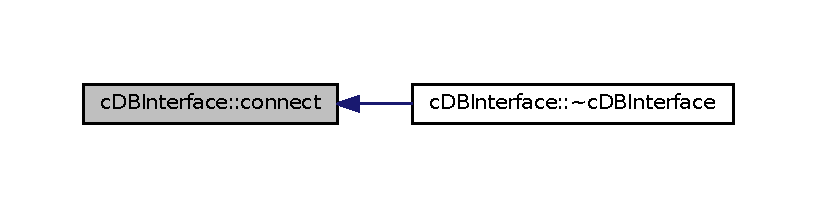
\includegraphics[width=350pt]{classc_d_b_interface_a1831bb8f93342190f26d83f35b4a988b_icgraph}
\end{center}
\end{figure}


\index{c\+D\+B\+Interface@{c\+D\+B\+Interface}!connected@{connected}}
\index{connected@{connected}!c\+D\+B\+Interface@{c\+D\+B\+Interface}}
\subsubsection[{\texorpdfstring{connected()}{connected()}}]{\setlength{\rightskip}{0pt plus 5cm}bool c\+D\+B\+Interface\+::connected (
\begin{DoxyParamCaption}
{}
\end{DoxyParamCaption}
)\hspace{0.3cm}{\ttfamily [inline]}}\hypertarget{classc_d_b_interface_a31ca3accfbd6dd1d2915440a94874b7b}{}\label{classc_d_b_interface_a31ca3accfbd6dd1d2915440a94874b7b}
\begin{DoxyNote}{Note}
This function must be derived by the subclass.
\end{DoxyNote}
\begin{DoxyReturn}{Returns}
bool true if connected, false otherwise. 
\end{DoxyReturn}


References m\+\_\+b\+Connected.

\index{c\+D\+B\+Interface@{c\+D\+B\+Interface}!init@{init}}
\index{init@{init}!c\+D\+B\+Interface@{c\+D\+B\+Interface}}
\subsubsection[{\texorpdfstring{init()=0}{init()=0}}]{\setlength{\rightskip}{0pt plus 5cm}virtual bool c\+D\+B\+Interface\+::init (
\begin{DoxyParamCaption}
{}
\end{DoxyParamCaption}
)\hspace{0.3cm}{\ttfamily [pure virtual]}}\hypertarget{classc_d_b_interface_a8baa6f378fb91dea077b38bd15be12c9}{}\label{classc_d_b_interface_a8baa6f378fb91dea077b38bd15be12c9}
\begin{DoxyNote}{Note}
This function must be derived by the subclass.
\end{DoxyNote}
\begin{DoxyReturn}{Returns}
bool true on success, false otherwise. 
\end{DoxyReturn}


Implemented in \hyperlink{classc_my_s_q_l_plugin_ab64cecb567902902ef25fd3cf7346a4c}{c\+My\+S\+Q\+L\+Plugin}, and \hyperlink{classc_s_q_lite_plugin_a5ed58193b879741aa561e6b5b24728a0}{c\+S\+Q\+Lite\+Plugin}.



Referenced by c\+Main\+Window\+::plugin\+D\+B\+Triggered(), and $\sim$c\+D\+B\+Interface().



Here is the caller graph for this function\+:
\nopagebreak
\begin{figure}[H]
\begin{center}
\leavevmode
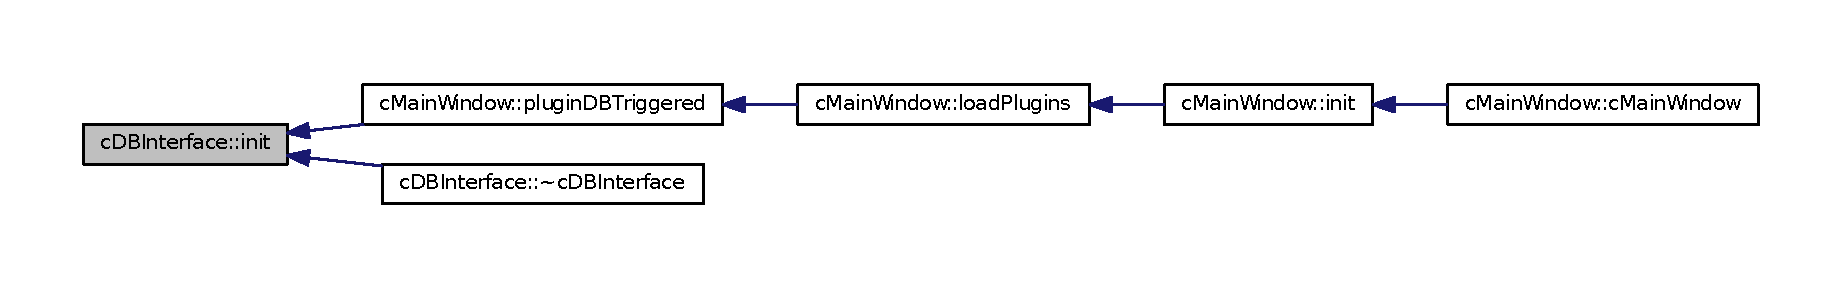
\includegraphics[width=350pt]{classc_d_b_interface_a8baa6f378fb91dea077b38bd15be12c9_icgraph}
\end{center}
\end{figure}


\index{c\+D\+B\+Interface@{c\+D\+B\+Interface}!last\+Error@{last\+Error}}
\index{last\+Error@{last\+Error}!c\+D\+B\+Interface@{c\+D\+B\+Interface}}
\subsubsection[{\texorpdfstring{last\+Error()}{lastError()}}]{\setlength{\rightskip}{0pt plus 5cm}Q\+String c\+D\+B\+Interface\+::last\+Error (
\begin{DoxyParamCaption}
{}
\end{DoxyParamCaption}
)\hspace{0.3cm}{\ttfamily [inline]}}\hypertarget{classc_d_b_interface_a280fe85549741179ce3a23b9f417c689}{}\label{classc_d_b_interface_a280fe85549741179ce3a23b9f417c689}
\begin{DoxyReturn}{Returns}
Q\+String error message of the last operation. 
\end{DoxyReturn}


\subsection{Member Data Documentation}
\index{c\+D\+B\+Interface@{c\+D\+B\+Interface}!m\+\_\+b\+Connected@{m\+\_\+b\+Connected}}
\index{m\+\_\+b\+Connected@{m\+\_\+b\+Connected}!c\+D\+B\+Interface@{c\+D\+B\+Interface}}
\subsubsection[{\texorpdfstring{m\+\_\+b\+Connected}{m_bConnected}}]{\setlength{\rightskip}{0pt plus 5cm}bool c\+D\+B\+Interface\+::m\+\_\+b\+Connected\hspace{0.3cm}{\ttfamily [protected]}}\hypertarget{classc_d_b_interface_a28d4d17206ee596e43e8c433c11c9282}{}\label{classc_d_b_interface_a28d4d17206ee596e43e8c433c11c9282}
holds the current connection status. 

Referenced by c\+My\+S\+Q\+L\+Plugin\+::config(), connected(), c\+S\+Q\+Lite\+Plugin\+::init(), c\+My\+S\+Q\+L\+Plugin\+::init(), c\+S\+Q\+Lite\+Plugin\+::open(), and c\+My\+S\+Q\+L\+Plugin\+::open().



The documentation for this class was generated from the following file\+:\begin{DoxyCompactItemize}
\item 
Kooky/\hyperlink{cdbinterface_8h}{cdbinterface.\+h}\end{DoxyCompactItemize}

\hypertarget{classc_ernaehrung_plugin}{}\section{c\+Ernaehrung\+Plugin Class Reference}
\label{classc_ernaehrung_plugin}\index{c\+Ernaehrung\+Plugin@{c\+Ernaehrung\+Plugin}}


{\ttfamily \#include $<$cernaehrungplugin.\+h$>$}



Inheritance diagram for c\+Ernaehrung\+Plugin\+:
\nopagebreak
\begin{figure}[H]
\begin{center}
\leavevmode
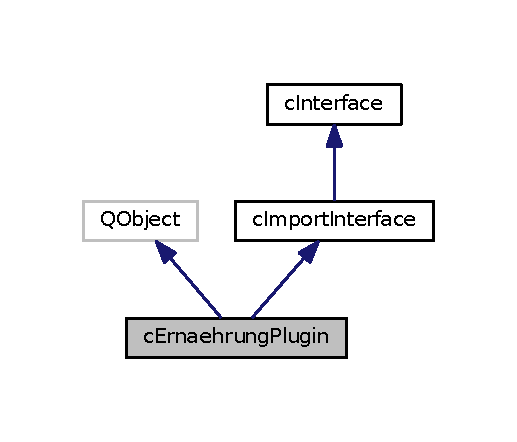
\includegraphics[width=248pt]{classc_ernaehrung_plugin__inherit__graph}
\end{center}
\end{figure}


Collaboration diagram for c\+Ernaehrung\+Plugin\+:
\nopagebreak
\begin{figure}[H]
\begin{center}
\leavevmode
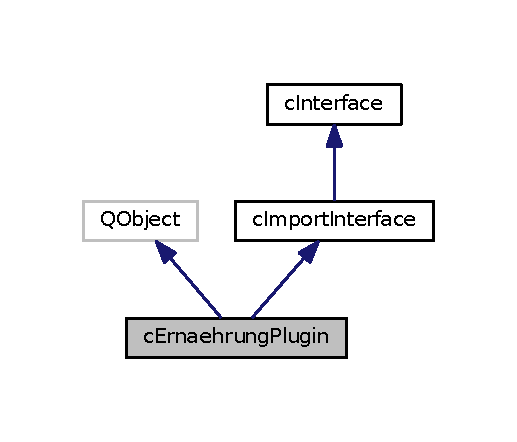
\includegraphics[width=248pt]{classc_ernaehrung_plugin__coll__graph}
\end{center}
\end{figure}
\subsection*{Public Member Functions}
\begin{DoxyCompactItemize}
\item 
qint16 \hyperlink{classc_ernaehrung_plugin_a44195e21ed764afb56bbcb4d64af1f3a}{plugin\+A\+P\+I\+Version} ()
\item 
Q\+String \hyperlink{classc_ernaehrung_plugin_a67ea2bef7e9d68fe3705baff59c9fec5}{plugin\+Name} ()
\item 
qint16 \hyperlink{classc_ernaehrung_plugin_a9f94e9684b541b55e67b87bff7a0a028}{plugin\+Version} ()
\item 
\hyperlink{classc_interface_a41462a3131755963add9ba3026e7d31a}{i\+Type} \hyperlink{classc_ernaehrung_plugin_aadc57be2d4fa422a9cadcbf647926700}{plugin\+Type} ()
\item 
bool \hyperlink{classc_ernaehrung_plugin_acbadba8cb20826f22cce60af8f4be98f}{config} ()
\item 
Q\+Map$<$ Q\+String, Q\+String $>$ \hyperlink{classc_ernaehrung_plugin_a9fef4cc5e1c59999833ffb4493cfae3e}{details\+Capability} ()
\item 
Q\+String\+List \hyperlink{classc_ernaehrung_plugin_aec19c86cca48415dbef841bc5b3cc15d}{search} (const Q\+String \&sz\+Search, const Q\+String \&sz\+Details=Q\+String(\char`\"{}\char`\"{}))
\item 
bool \hyperlink{classc_ernaehrung_plugin_a2d688c0a56bed5b8f233dd5890a96a3d}{load} (qint16 i\+Index)
\item 
qreal \hyperlink{classc_ernaehrung_plugin_a8b4bb34247562c26687bb33e6369eb25}{value} (\hyperlink{classc_ingredient_acf023723841ec66cd6368a25e3174a28}{c\+Ingredient\+::i\+Ingredient} i)
\item 
Q\+String \hyperlink{classc_ernaehrung_plugin_a24c04c0b98fb4186e5b5b012662b39ed}{ingredient\+Name} ()
\end{DoxyCompactItemize}
\subsection*{Private Attributes}
\begin{DoxyCompactItemize}
\item 
Q\+String\+List \hyperlink{classc_ernaehrung_plugin_a58692dcfff3d8f9da462b90fbf12db06}{m\+\_\+sz\+Urls}
\item 
Q\+String\+List \hyperlink{classc_ernaehrung_plugin_aa586d90efc11b68dce605fdf1a45910d}{m\+\_\+sz\+Ingredients}
\item 
qint16 \hyperlink{classc_ernaehrung_plugin_a947339aef16691c4165c7eb1869d3b7e}{m\+\_\+i\+Loaded\+Index}
\end{DoxyCompactItemize}
\subsection*{Additional Inherited Members}


\subsection{Member Function Documentation}
\index{c\+Ernaehrung\+Plugin@{c\+Ernaehrung\+Plugin}!config@{config}}
\index{config@{config}!c\+Ernaehrung\+Plugin@{c\+Ernaehrung\+Plugin}}
\subsubsection[{\texorpdfstring{config()}{config()}}]{\setlength{\rightskip}{0pt plus 5cm}bool c\+Ernaehrung\+Plugin\+::config (
\begin{DoxyParamCaption}
{}
\end{DoxyParamCaption}
)\hspace{0.3cm}{\ttfamily [virtual]}}\hypertarget{classc_ernaehrung_plugin_acbadba8cb20826f22cce60af8f4be98f}{}\label{classc_ernaehrung_plugin_acbadba8cb20826f22cce60af8f4be98f}
\begin{DoxyReturn}{Returns}
bool 
\end{DoxyReturn}


Implements \hyperlink{classc_interface_a040fbd069a2c2356faeda1c2d9ac88df}{c\+Interface}.



Referenced by plugin\+Type().



Here is the caller graph for this function\+:
\nopagebreak
\begin{figure}[H]
\begin{center}
\leavevmode
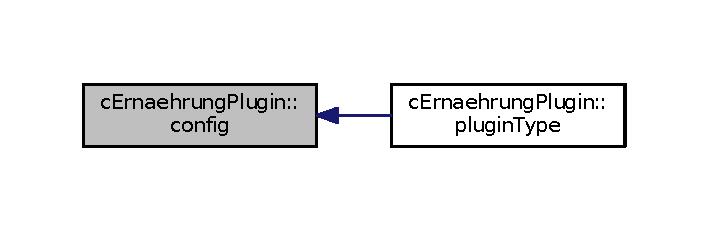
\includegraphics[width=340pt]{classc_ernaehrung_plugin_acbadba8cb20826f22cce60af8f4be98f_icgraph}
\end{center}
\end{figure}


\index{c\+Ernaehrung\+Plugin@{c\+Ernaehrung\+Plugin}!details\+Capability@{details\+Capability}}
\index{details\+Capability@{details\+Capability}!c\+Ernaehrung\+Plugin@{c\+Ernaehrung\+Plugin}}
\subsubsection[{\texorpdfstring{details\+Capability()}{detailsCapability()}}]{\setlength{\rightskip}{0pt plus 5cm}Q\+Map$<$ Q\+String, Q\+String $>$ c\+Ernaehrung\+Plugin\+::details\+Capability (
\begin{DoxyParamCaption}
{}
\end{DoxyParamCaption}
)\hspace{0.3cm}{\ttfamily [virtual]}}\hypertarget{classc_ernaehrung_plugin_a9fef4cc5e1c59999833ffb4493cfae3e}{}\label{classc_ernaehrung_plugin_a9fef4cc5e1c59999833ffb4493cfae3e}
\begin{DoxyReturn}{Returns}
Q\+Map$<$\+Q\+String, Q\+String$>$ 
\end{DoxyReturn}


Implements \hyperlink{classc_import_interface_a4ec2f198f8488e7daf2e93cf637a580d}{c\+Import\+Interface}.



Referenced by plugin\+Type().



Here is the caller graph for this function\+:
\nopagebreak
\begin{figure}[H]
\begin{center}
\leavevmode
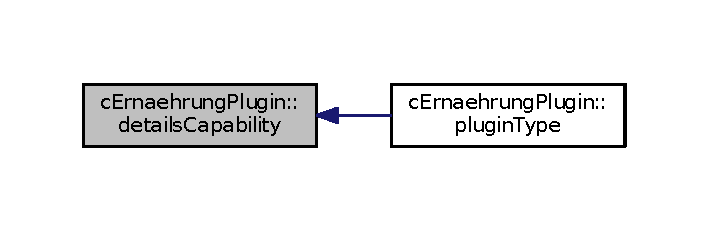
\includegraphics[width=340pt]{classc_ernaehrung_plugin_a9fef4cc5e1c59999833ffb4493cfae3e_icgraph}
\end{center}
\end{figure}


\index{c\+Ernaehrung\+Plugin@{c\+Ernaehrung\+Plugin}!ingredient\+Name@{ingredient\+Name}}
\index{ingredient\+Name@{ingredient\+Name}!c\+Ernaehrung\+Plugin@{c\+Ernaehrung\+Plugin}}
\subsubsection[{\texorpdfstring{ingredient\+Name()}{ingredientName()}}]{\setlength{\rightskip}{0pt plus 5cm}Q\+String c\+Ernaehrung\+Plugin\+::ingredient\+Name (
\begin{DoxyParamCaption}
{}
\end{DoxyParamCaption}
)\hspace{0.3cm}{\ttfamily [virtual]}}\hypertarget{classc_ernaehrung_plugin_a24c04c0b98fb4186e5b5b012662b39ed}{}\label{classc_ernaehrung_plugin_a24c04c0b98fb4186e5b5b012662b39ed}
\begin{DoxyReturn}{Returns}
Q\+String 
\end{DoxyReturn}


Implements \hyperlink{classc_import_interface_af3f569b605787021a919816978f229bc}{c\+Import\+Interface}.



Referenced by plugin\+Type().



Here is the caller graph for this function\+:
\nopagebreak
\begin{figure}[H]
\begin{center}
\leavevmode
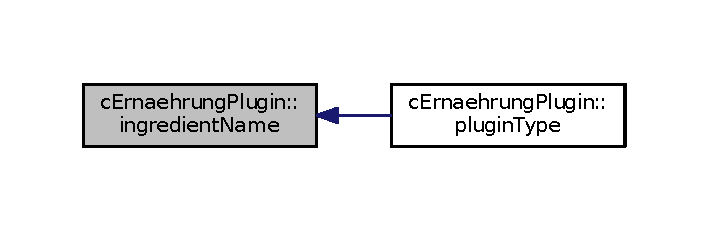
\includegraphics[width=340pt]{classc_ernaehrung_plugin_a24c04c0b98fb4186e5b5b012662b39ed_icgraph}
\end{center}
\end{figure}


\index{c\+Ernaehrung\+Plugin@{c\+Ernaehrung\+Plugin}!load@{load}}
\index{load@{load}!c\+Ernaehrung\+Plugin@{c\+Ernaehrung\+Plugin}}
\subsubsection[{\texorpdfstring{load(qint16 i\+Index)}{load(qint16 iIndex)}}]{\setlength{\rightskip}{0pt plus 5cm}bool c\+Ernaehrung\+Plugin\+::load (
\begin{DoxyParamCaption}
\item[{qint16}]{i\+Index}
\end{DoxyParamCaption}
)\hspace{0.3cm}{\ttfamily [virtual]}}\hypertarget{classc_ernaehrung_plugin_a2d688c0a56bed5b8f233dd5890a96a3d}{}\label{classc_ernaehrung_plugin_a2d688c0a56bed5b8f233dd5890a96a3d}

\begin{DoxyParams}{Parameters}
{\em i\+Index} & \\
\hline
\end{DoxyParams}
\begin{DoxyReturn}{Returns}
bool 
\end{DoxyReturn}


Implements \hyperlink{classc_import_interface_a728bcb2a636f78bae2fe7e128a18e983}{c\+Import\+Interface}.



References tag\+V\+A\+L\+U\+E\+S\+::d\+Value, tag\+V\+A\+L\+U\+E\+S\+::sz\+Search, and to\+Value().



Referenced by plugin\+Type().



Here is the call graph for this function\+:
\nopagebreak
\begin{figure}[H]
\begin{center}
\leavevmode
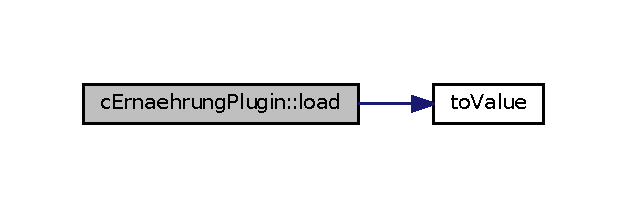
\includegraphics[width=301pt]{classc_ernaehrung_plugin_a2d688c0a56bed5b8f233dd5890a96a3d_cgraph}
\end{center}
\end{figure}




Here is the caller graph for this function\+:
\nopagebreak
\begin{figure}[H]
\begin{center}
\leavevmode
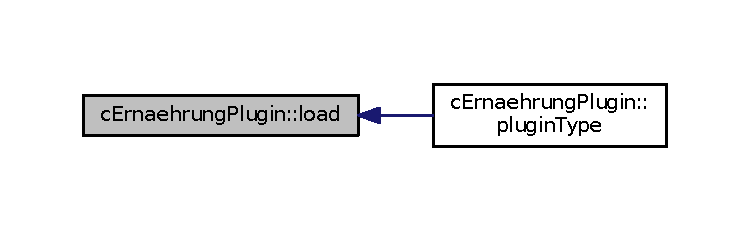
\includegraphics[width=350pt]{classc_ernaehrung_plugin_a2d688c0a56bed5b8f233dd5890a96a3d_icgraph}
\end{center}
\end{figure}


\index{c\+Ernaehrung\+Plugin@{c\+Ernaehrung\+Plugin}!plugin\+A\+P\+I\+Version@{plugin\+A\+P\+I\+Version}}
\index{plugin\+A\+P\+I\+Version@{plugin\+A\+P\+I\+Version}!c\+Ernaehrung\+Plugin@{c\+Ernaehrung\+Plugin}}
\subsubsection[{\texorpdfstring{plugin\+A\+P\+I\+Version()}{pluginAPIVersion()}}]{\setlength{\rightskip}{0pt plus 5cm}qint16 c\+Ernaehrung\+Plugin\+::plugin\+A\+P\+I\+Version (
\begin{DoxyParamCaption}
{}
\end{DoxyParamCaption}
)\hspace{0.3cm}{\ttfamily [inline]}, {\ttfamily [virtual]}}\hypertarget{classc_ernaehrung_plugin_a44195e21ed764afb56bbcb4d64af1f3a}{}\label{classc_ernaehrung_plugin_a44195e21ed764afb56bbcb4d64af1f3a}
\begin{DoxyReturn}{Returns}
qint16 
\end{DoxyReturn}


Implements \hyperlink{classc_interface_a615b50a526c2d4ca73b13f8991371813}{c\+Interface}.

\index{c\+Ernaehrung\+Plugin@{c\+Ernaehrung\+Plugin}!plugin\+Name@{plugin\+Name}}
\index{plugin\+Name@{plugin\+Name}!c\+Ernaehrung\+Plugin@{c\+Ernaehrung\+Plugin}}
\subsubsection[{\texorpdfstring{plugin\+Name()}{pluginName()}}]{\setlength{\rightskip}{0pt plus 5cm}Q\+String c\+Ernaehrung\+Plugin\+::plugin\+Name (
\begin{DoxyParamCaption}
{}
\end{DoxyParamCaption}
)\hspace{0.3cm}{\ttfamily [inline]}, {\ttfamily [virtual]}}\hypertarget{classc_ernaehrung_plugin_a67ea2bef7e9d68fe3705baff59c9fec5}{}\label{classc_ernaehrung_plugin_a67ea2bef7e9d68fe3705baff59c9fec5}
\begin{DoxyReturn}{Returns}
Q\+String 
\end{DoxyReturn}


Implements \hyperlink{classc_interface_a17e5a0cf99317ab45f624e68b4a6ecca}{c\+Interface}.

\index{c\+Ernaehrung\+Plugin@{c\+Ernaehrung\+Plugin}!plugin\+Type@{plugin\+Type}}
\index{plugin\+Type@{plugin\+Type}!c\+Ernaehrung\+Plugin@{c\+Ernaehrung\+Plugin}}
\subsubsection[{\texorpdfstring{plugin\+Type()}{pluginType()}}]{\setlength{\rightskip}{0pt plus 5cm}{\bf i\+Type} c\+Ernaehrung\+Plugin\+::plugin\+Type (
\begin{DoxyParamCaption}
{}
\end{DoxyParamCaption}
)\hspace{0.3cm}{\ttfamily [inline]}, {\ttfamily [virtual]}}\hypertarget{classc_ernaehrung_plugin_aadc57be2d4fa422a9cadcbf647926700}{}\label{classc_ernaehrung_plugin_aadc57be2d4fa422a9cadcbf647926700}
\begin{DoxyReturn}{Returns}
i\+Type 
\end{DoxyReturn}


Implements \hyperlink{classc_interface_af5e408cdaff527a872ce6d02a96301a4}{c\+Interface}.



References config(), details\+Capability(), ingredient\+Name(), c\+Interface\+::i\+Type\+Import, load(), search(), and value().



Here is the call graph for this function\+:
\nopagebreak
\begin{figure}[H]
\begin{center}
\leavevmode
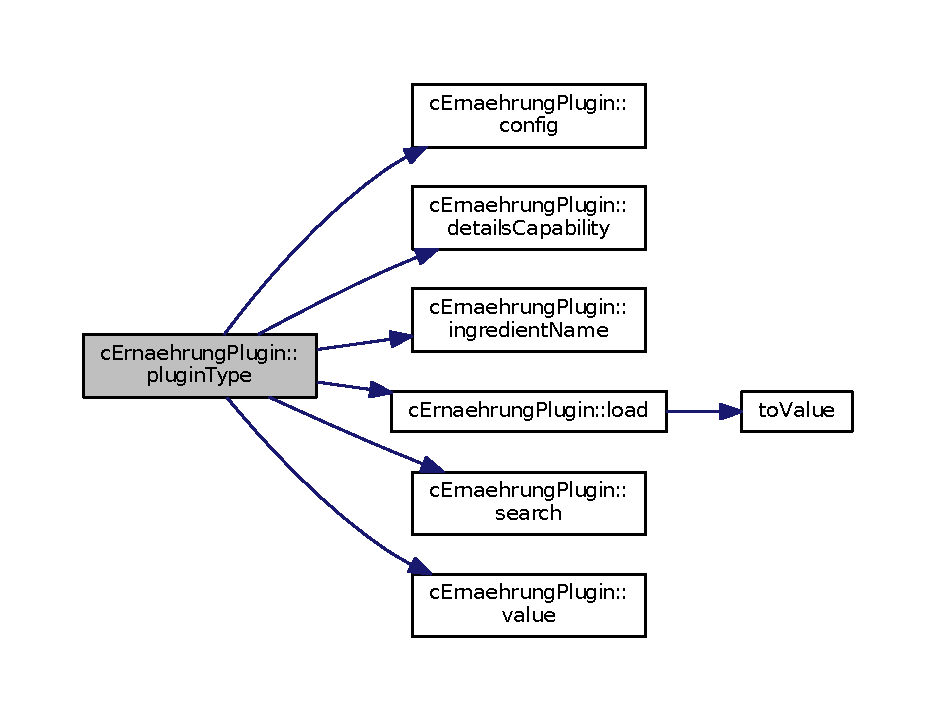
\includegraphics[width=350pt]{classc_ernaehrung_plugin_aadc57be2d4fa422a9cadcbf647926700_cgraph}
\end{center}
\end{figure}


\index{c\+Ernaehrung\+Plugin@{c\+Ernaehrung\+Plugin}!plugin\+Version@{plugin\+Version}}
\index{plugin\+Version@{plugin\+Version}!c\+Ernaehrung\+Plugin@{c\+Ernaehrung\+Plugin}}
\subsubsection[{\texorpdfstring{plugin\+Version()}{pluginVersion()}}]{\setlength{\rightskip}{0pt plus 5cm}qint16 c\+Ernaehrung\+Plugin\+::plugin\+Version (
\begin{DoxyParamCaption}
{}
\end{DoxyParamCaption}
)\hspace{0.3cm}{\ttfamily [inline]}, {\ttfamily [virtual]}}\hypertarget{classc_ernaehrung_plugin_a9f94e9684b541b55e67b87bff7a0a028}{}\label{classc_ernaehrung_plugin_a9f94e9684b541b55e67b87bff7a0a028}
\begin{DoxyReturn}{Returns}
qint16 
\end{DoxyReturn}


Implements \hyperlink{classc_interface_aadc382036174c2a25bb2c23733830d33}{c\+Interface}.

\index{c\+Ernaehrung\+Plugin@{c\+Ernaehrung\+Plugin}!search@{search}}
\index{search@{search}!c\+Ernaehrung\+Plugin@{c\+Ernaehrung\+Plugin}}
\subsubsection[{\texorpdfstring{search(const Q\+String \&sz\+Search, const Q\+String \&sz\+Details=\+Q\+String(""""))}{search(const QString &szSearch, const QString &szDetails=QString(""))}}]{\setlength{\rightskip}{0pt plus 5cm}Q\+String\+List c\+Ernaehrung\+Plugin\+::search (
\begin{DoxyParamCaption}
\item[{const Q\+String \&}]{sz\+Search, }
\item[{const Q\+String \&}]{sz\+Details = {\ttfamily QString(\char`\"{}\char`\"{})}}
\end{DoxyParamCaption}
)\hspace{0.3cm}{\ttfamily [virtual]}}\hypertarget{classc_ernaehrung_plugin_aec19c86cca48415dbef841bc5b3cc15d}{}\label{classc_ernaehrung_plugin_aec19c86cca48415dbef841bc5b3cc15d}

\begin{DoxyParams}{Parameters}
{\em sz\+Search} & \\
\hline
{\em sz\+Details} & \\
\hline
\end{DoxyParams}
\begin{DoxyReturn}{Returns}
Q\+String\+List 
\end{DoxyReturn}


Implements \hyperlink{classc_import_interface_a8b48a3821674ff15d7eaf4e03c55409f}{c\+Import\+Interface}.



Referenced by plugin\+Type().



Here is the caller graph for this function\+:
\nopagebreak
\begin{figure}[H]
\begin{center}
\leavevmode
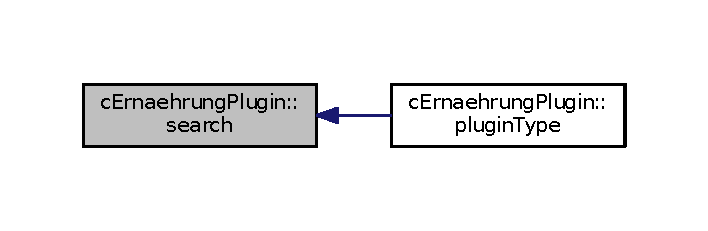
\includegraphics[width=340pt]{classc_ernaehrung_plugin_aec19c86cca48415dbef841bc5b3cc15d_icgraph}
\end{center}
\end{figure}


\index{c\+Ernaehrung\+Plugin@{c\+Ernaehrung\+Plugin}!value@{value}}
\index{value@{value}!c\+Ernaehrung\+Plugin@{c\+Ernaehrung\+Plugin}}
\subsubsection[{\texorpdfstring{value(c\+Ingredient\+::i\+Ingredient i)}{value(cIngredient::iIngredient i)}}]{\setlength{\rightskip}{0pt plus 5cm}qreal c\+Ernaehrung\+Plugin\+::value (
\begin{DoxyParamCaption}
\item[{{\bf c\+Ingredient\+::i\+Ingredient}}]{i}
\end{DoxyParamCaption}
)\hspace{0.3cm}{\ttfamily [virtual]}}\hypertarget{classc_ernaehrung_plugin_a8b4bb34247562c26687bb33e6369eb25}{}\label{classc_ernaehrung_plugin_a8b4bb34247562c26687bb33e6369eb25}

\begin{DoxyParams}{Parameters}
{\em i} & \\
\hline
\end{DoxyParams}
\begin{DoxyReturn}{Returns}
qreal 
\end{DoxyReturn}


Implements \hyperlink{classc_import_interface_a7a8dbe6a164549272d748d2f77aebc42}{c\+Import\+Interface}.



References tag\+V\+A\+L\+U\+E\+S\+::d\+Value, and tag\+V\+A\+L\+U\+E\+S\+::i\+Ingredient.



Referenced by plugin\+Type().



Here is the caller graph for this function\+:
\nopagebreak
\begin{figure}[H]
\begin{center}
\leavevmode
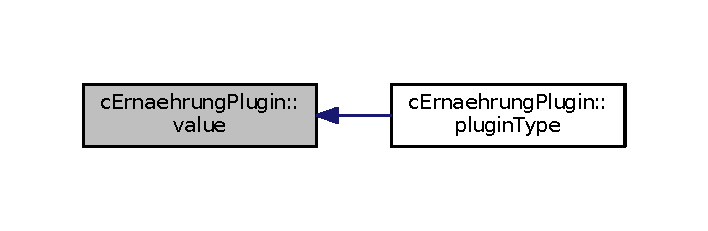
\includegraphics[width=340pt]{classc_ernaehrung_plugin_a8b4bb34247562c26687bb33e6369eb25_icgraph}
\end{center}
\end{figure}




\subsection{Member Data Documentation}
\index{c\+Ernaehrung\+Plugin@{c\+Ernaehrung\+Plugin}!m\+\_\+i\+Loaded\+Index@{m\+\_\+i\+Loaded\+Index}}
\index{m\+\_\+i\+Loaded\+Index@{m\+\_\+i\+Loaded\+Index}!c\+Ernaehrung\+Plugin@{c\+Ernaehrung\+Plugin}}
\subsubsection[{\texorpdfstring{m\+\_\+i\+Loaded\+Index}{m_iLoadedIndex}}]{\setlength{\rightskip}{0pt plus 5cm}qint16 c\+Ernaehrung\+Plugin\+::m\+\_\+i\+Loaded\+Index\hspace{0.3cm}{\ttfamily [private]}}\hypertarget{classc_ernaehrung_plugin_a947339aef16691c4165c7eb1869d3b7e}{}\label{classc_ernaehrung_plugin_a947339aef16691c4165c7eb1869d3b7e}
T\+O\+DO\+: describe \index{c\+Ernaehrung\+Plugin@{c\+Ernaehrung\+Plugin}!m\+\_\+sz\+Ingredients@{m\+\_\+sz\+Ingredients}}
\index{m\+\_\+sz\+Ingredients@{m\+\_\+sz\+Ingredients}!c\+Ernaehrung\+Plugin@{c\+Ernaehrung\+Plugin}}
\subsubsection[{\texorpdfstring{m\+\_\+sz\+Ingredients}{m_szIngredients}}]{\setlength{\rightskip}{0pt plus 5cm}Q\+String\+List c\+Ernaehrung\+Plugin\+::m\+\_\+sz\+Ingredients\hspace{0.3cm}{\ttfamily [private]}}\hypertarget{classc_ernaehrung_plugin_aa586d90efc11b68dce605fdf1a45910d}{}\label{classc_ernaehrung_plugin_aa586d90efc11b68dce605fdf1a45910d}
T\+O\+DO\+: describe \index{c\+Ernaehrung\+Plugin@{c\+Ernaehrung\+Plugin}!m\+\_\+sz\+Urls@{m\+\_\+sz\+Urls}}
\index{m\+\_\+sz\+Urls@{m\+\_\+sz\+Urls}!c\+Ernaehrung\+Plugin@{c\+Ernaehrung\+Plugin}}
\subsubsection[{\texorpdfstring{m\+\_\+sz\+Urls}{m_szUrls}}]{\setlength{\rightskip}{0pt plus 5cm}Q\+String\+List c\+Ernaehrung\+Plugin\+::m\+\_\+sz\+Urls\hspace{0.3cm}{\ttfamily [private]}}\hypertarget{classc_ernaehrung_plugin_a58692dcfff3d8f9da462b90fbf12db06}{}\label{classc_ernaehrung_plugin_a58692dcfff3d8f9da462b90fbf12db06}
T\+O\+DO\+: describe 

The documentation for this class was generated from the following files\+:\begin{DoxyCompactItemize}
\item 
i\+Ernaehrung/\hyperlink{cernaehrungplugin_8h}{cernaehrungplugin.\+h}\item 
i\+Ernaehrung/\hyperlink{cernaehrungplugin_8cpp}{cernaehrungplugin.\+cpp}\end{DoxyCompactItemize}

\hypertarget{classc_import_ingredient_dialog}{}\section{c\+Import\+Ingredient\+Dialog Class Reference}
\label{classc_import_ingredient_dialog}\index{c\+Import\+Ingredient\+Dialog@{c\+Import\+Ingredient\+Dialog}}


This dialog imports ingredients based on the selected import plugin.  




{\ttfamily \#include $<$cimportingredientdialog.\+h$>$}



Inheritance diagram for c\+Import\+Ingredient\+Dialog\+:
\nopagebreak
\begin{figure}[H]
\begin{center}
\leavevmode
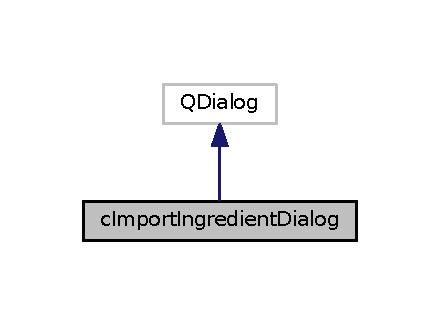
\includegraphics[width=211pt]{classc_import_ingredient_dialog__inherit__graph}
\end{center}
\end{figure}


Collaboration diagram for c\+Import\+Ingredient\+Dialog\+:
\nopagebreak
\begin{figure}[H]
\begin{center}
\leavevmode
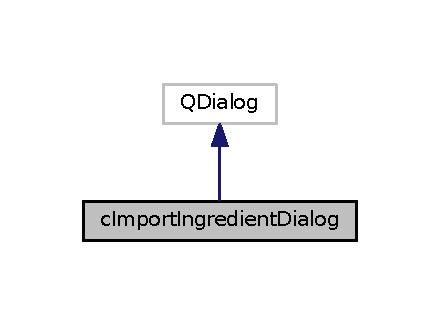
\includegraphics[width=211pt]{classc_import_ingredient_dialog__coll__graph}
\end{center}
\end{figure}
\subsection*{Public Member Functions}
\begin{DoxyCompactItemize}
\item 
\hyperlink{classc_import_ingredient_dialog_a4bea50afa976e55633017756cef4443e}{c\+Import\+Ingredient\+Dialog} (Q\+Widget $\ast$parent=0)
\item 
\hyperlink{classc_import_ingredient_dialog_a07b1bee5504a45413b3736d757bf2c5e}{$\sim$c\+Import\+Ingredient\+Dialog} ()
\item 
void \hyperlink{classc_import_ingredient_dialog_ad710be68582d34c43a399b4764c0434a}{set\+Plugin\+List} (const Q\+List$<$ \hyperlink{classc_plugin}{c\+Plugin} $\ast$ $>$ plugin\+List)
\end{DoxyCompactItemize}
\subsection*{Protected Member Functions}
\begin{DoxyCompactItemize}
\item 
Q\+Standard\+Item $\ast$ \hyperlink{classc_import_ingredient_dialog_ae0115db7ba009ecbfcd0af68f4e71e3d}{add\+Group} (const Q\+String \&group)
\item 
void \hyperlink{classc_import_ingredient_dialog_acd246954f20eba6d65d233adb3a9c293}{init} ()
\item 
void \hyperlink{classc_import_ingredient_dialog_adf78505fef0d070021878b885fd5a0ea}{init\+Ingredient\+List} ()
\item 
void \hyperlink{classc_import_ingredient_dialog_a6158a639b7b11973e84ddb3ca7d9aeb6}{init\+Ingredient\+Details} ()
\end{DoxyCompactItemize}
\subsection*{Protected Attributes}
\begin{DoxyCompactItemize}
\item 
Q\+List$<$ \hyperlink{classc_plugin}{c\+Plugin} $\ast$ $>$ \hyperlink{classc_import_ingredient_dialog_ad5795b238430db474ae852bfbb493578}{m\+\_\+plugin\+List}
\end{DoxyCompactItemize}
\subsection*{Private Slots}
\begin{DoxyCompactItemize}
\item 
void \hyperlink{classc_import_ingredient_dialog_aad6f67e1420e7ceba52d6ea72bf70e88}{on\+\_\+m\+\_\+lp\+Search\+Button\+\_\+clicked} ()
\item 
void \hyperlink{classc_import_ingredient_dialog_a2b5fa289051ab3b18e71f7e2cb7573b3}{on\+\_\+m\+\_\+lp\+Search\+String\+\_\+text\+Changed} (const Q\+String \&arg1)
\item 
void \hyperlink{classc_import_ingredient_dialog_a7aaca4be76facdc5c90fd321825a6289}{on\+Ingredient\+List\+Selection\+Changed} (const Q\+Item\+Selection \&selected, const Q\+Item\+Selection \&deselected)
\end{DoxyCompactItemize}
\subsection*{Private Attributes}
\begin{DoxyCompactItemize}
\item 
Ui\+::c\+Import\+Ingredient\+Dialog $\ast$ \hyperlink{classc_import_ingredient_dialog_a80da8aa411eb8da3a692693445e64408}{ui}
\item 
Q\+Standard\+Item\+Model $\ast$ \hyperlink{classc_import_ingredient_dialog_a0fe1def4e950a1f06a14f28ff7d9ba6a}{m\+\_\+lp\+Ingredient\+List\+Model}
\item 
Q\+Standard\+Item\+Model $\ast$ \hyperlink{classc_import_ingredient_dialog_a9fcdb59fa6c5fc9b65c4db1e43afb3db}{m\+\_\+lp\+Ingredient\+Details\+Model}
\end{DoxyCompactItemize}


\subsection{Detailed Description}
This dialog imports ingredients based on the selected import plugin.

\begin{DoxyNote}{Note}

\end{DoxyNote}
\begin{DoxyAuthor}{Author}
Herwig Birke
\end{DoxyAuthor}
\begin{DoxyVersion}{Version}
1.\+0
\end{DoxyVersion}
\begin{DoxyDate}{Date}
2016/02/09 
\end{DoxyDate}


\subsection{Constructor \& Destructor Documentation}
\index{c\+Import\+Ingredient\+Dialog@{c\+Import\+Ingredient\+Dialog}!c\+Import\+Ingredient\+Dialog@{c\+Import\+Ingredient\+Dialog}}
\index{c\+Import\+Ingredient\+Dialog@{c\+Import\+Ingredient\+Dialog}!c\+Import\+Ingredient\+Dialog@{c\+Import\+Ingredient\+Dialog}}
\subsubsection[{\texorpdfstring{c\+Import\+Ingredient\+Dialog(\+Q\+Widget $\ast$parent=0)}{cImportIngredientDialog(QWidget *parent=0)}}]{\setlength{\rightskip}{0pt plus 5cm}c\+Import\+Ingredient\+Dialog\+::c\+Import\+Ingredient\+Dialog (
\begin{DoxyParamCaption}
\item[{Q\+Widget $\ast$}]{parent = {\ttfamily 0}}
\end{DoxyParamCaption}
)\hspace{0.3cm}{\ttfamily [explicit]}}\hypertarget{classc_import_ingredient_dialog_a4bea50afa976e55633017756cef4443e}{}\label{classc_import_ingredient_dialog_a4bea50afa976e55633017756cef4443e}

\begin{DoxyParams}{Parameters}
{\em parent} & \\
\hline
\end{DoxyParams}


References init().



Here is the call graph for this function\+:
\nopagebreak
\begin{figure}[H]
\begin{center}
\leavevmode
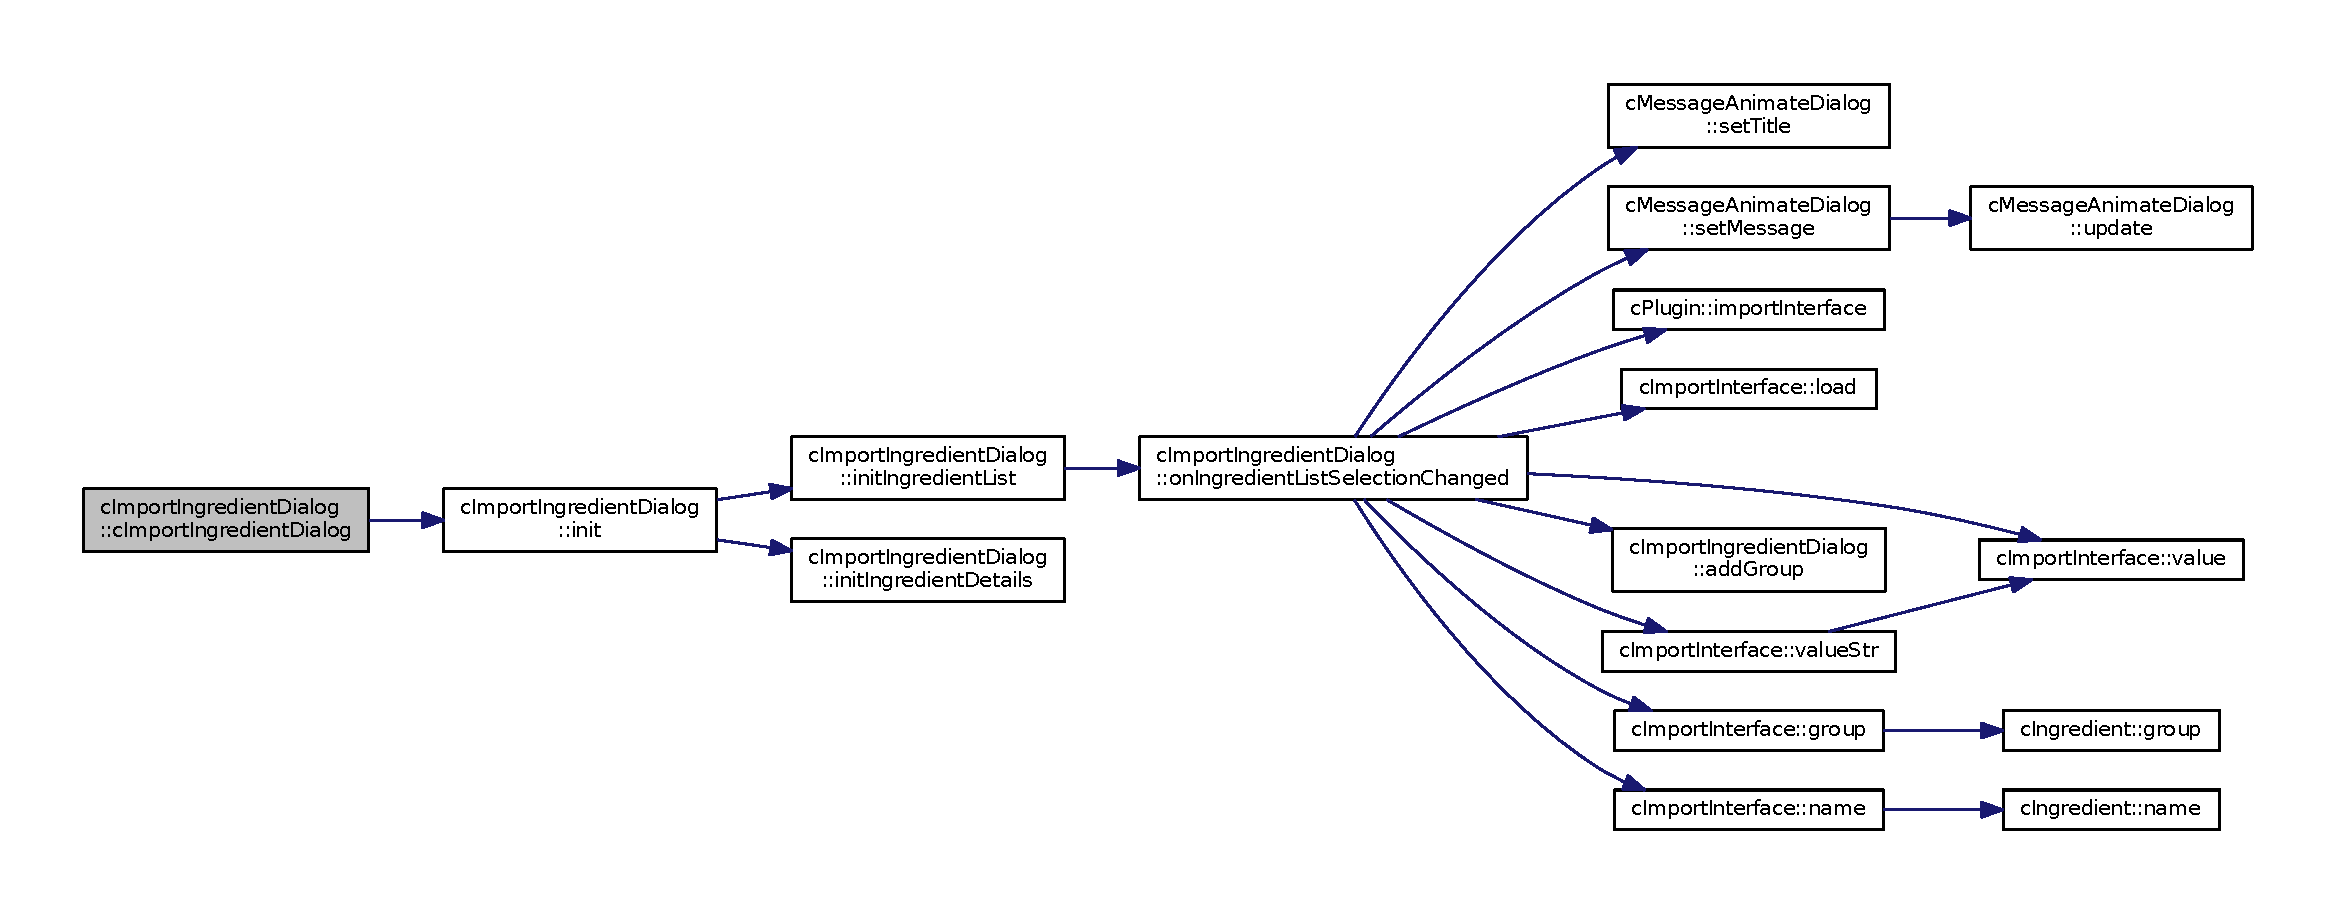
\includegraphics[width=350pt]{classc_import_ingredient_dialog_a4bea50afa976e55633017756cef4443e_cgraph}
\end{center}
\end{figure}


\index{c\+Import\+Ingredient\+Dialog@{c\+Import\+Ingredient\+Dialog}!````~c\+Import\+Ingredient\+Dialog@{$\sim$c\+Import\+Ingredient\+Dialog}}
\index{````~c\+Import\+Ingredient\+Dialog@{$\sim$c\+Import\+Ingredient\+Dialog}!c\+Import\+Ingredient\+Dialog@{c\+Import\+Ingredient\+Dialog}}
\subsubsection[{\texorpdfstring{$\sim$c\+Import\+Ingredient\+Dialog()}{~cImportIngredientDialog()}}]{\setlength{\rightskip}{0pt plus 5cm}c\+Import\+Ingredient\+Dialog\+::$\sim$c\+Import\+Ingredient\+Dialog (
\begin{DoxyParamCaption}
{}
\end{DoxyParamCaption}
)}\hypertarget{classc_import_ingredient_dialog_a07b1bee5504a45413b3736d757bf2c5e}{}\label{classc_import_ingredient_dialog_a07b1bee5504a45413b3736d757bf2c5e}


References ui.



\subsection{Member Function Documentation}
\index{c\+Import\+Ingredient\+Dialog@{c\+Import\+Ingredient\+Dialog}!add\+Group@{add\+Group}}
\index{add\+Group@{add\+Group}!c\+Import\+Ingredient\+Dialog@{c\+Import\+Ingredient\+Dialog}}
\subsubsection[{\texorpdfstring{add\+Group(const Q\+String \&group)}{addGroup(const QString &group)}}]{\setlength{\rightskip}{0pt plus 5cm}Q\+Standard\+Item $\ast$ c\+Import\+Ingredient\+Dialog\+::add\+Group (
\begin{DoxyParamCaption}
\item[{const Q\+String \&}]{group}
\end{DoxyParamCaption}
)\hspace{0.3cm}{\ttfamily [protected]}}\hypertarget{classc_import_ingredient_dialog_ae0115db7ba009ecbfcd0af68f4e71e3d}{}\label{classc_import_ingredient_dialog_ae0115db7ba009ecbfcd0af68f4e71e3d}

\begin{DoxyParams}{Parameters}
{\em group} & \\
\hline
\end{DoxyParams}
\begin{DoxyReturn}{Returns}
Q\+Standard\+Item 
\end{DoxyReturn}


References m\+\_\+lp\+Ingredient\+Details\+Model.



Referenced by on\+Ingredient\+List\+Selection\+Changed().



Here is the caller graph for this function\+:
\nopagebreak
\begin{figure}[H]
\begin{center}
\leavevmode
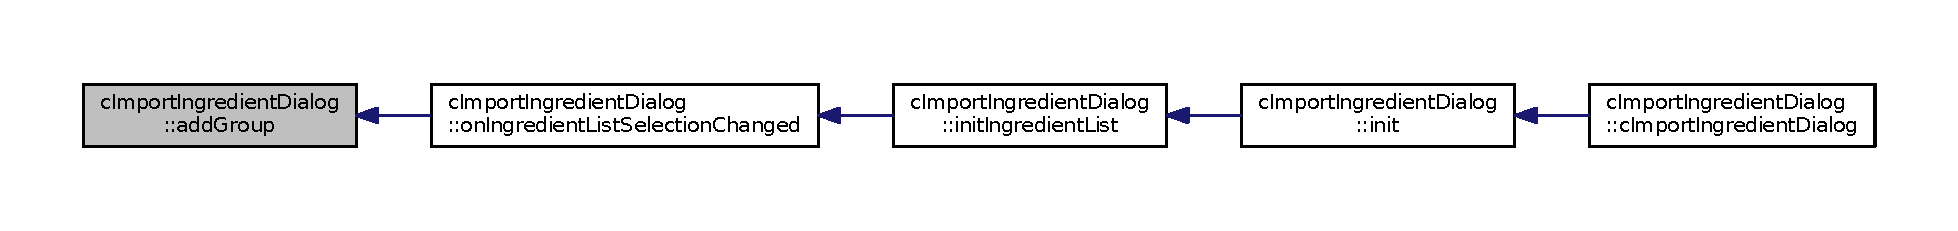
\includegraphics[width=350pt]{classc_import_ingredient_dialog_ae0115db7ba009ecbfcd0af68f4e71e3d_icgraph}
\end{center}
\end{figure}


\index{c\+Import\+Ingredient\+Dialog@{c\+Import\+Ingredient\+Dialog}!init@{init}}
\index{init@{init}!c\+Import\+Ingredient\+Dialog@{c\+Import\+Ingredient\+Dialog}}
\subsubsection[{\texorpdfstring{init()}{init()}}]{\setlength{\rightskip}{0pt plus 5cm}void c\+Import\+Ingredient\+Dialog\+::init (
\begin{DoxyParamCaption}
{}
\end{DoxyParamCaption}
)\hspace{0.3cm}{\ttfamily [protected]}}\hypertarget{classc_import_ingredient_dialog_acd246954f20eba6d65d233adb3a9c293}{}\label{classc_import_ingredient_dialog_acd246954f20eba6d65d233adb3a9c293}


References init\+Ingredient\+Details(), init\+Ingredient\+List(), and ui.



Referenced by c\+Import\+Ingredient\+Dialog().



Here is the call graph for this function\+:
\nopagebreak
\begin{figure}[H]
\begin{center}
\leavevmode
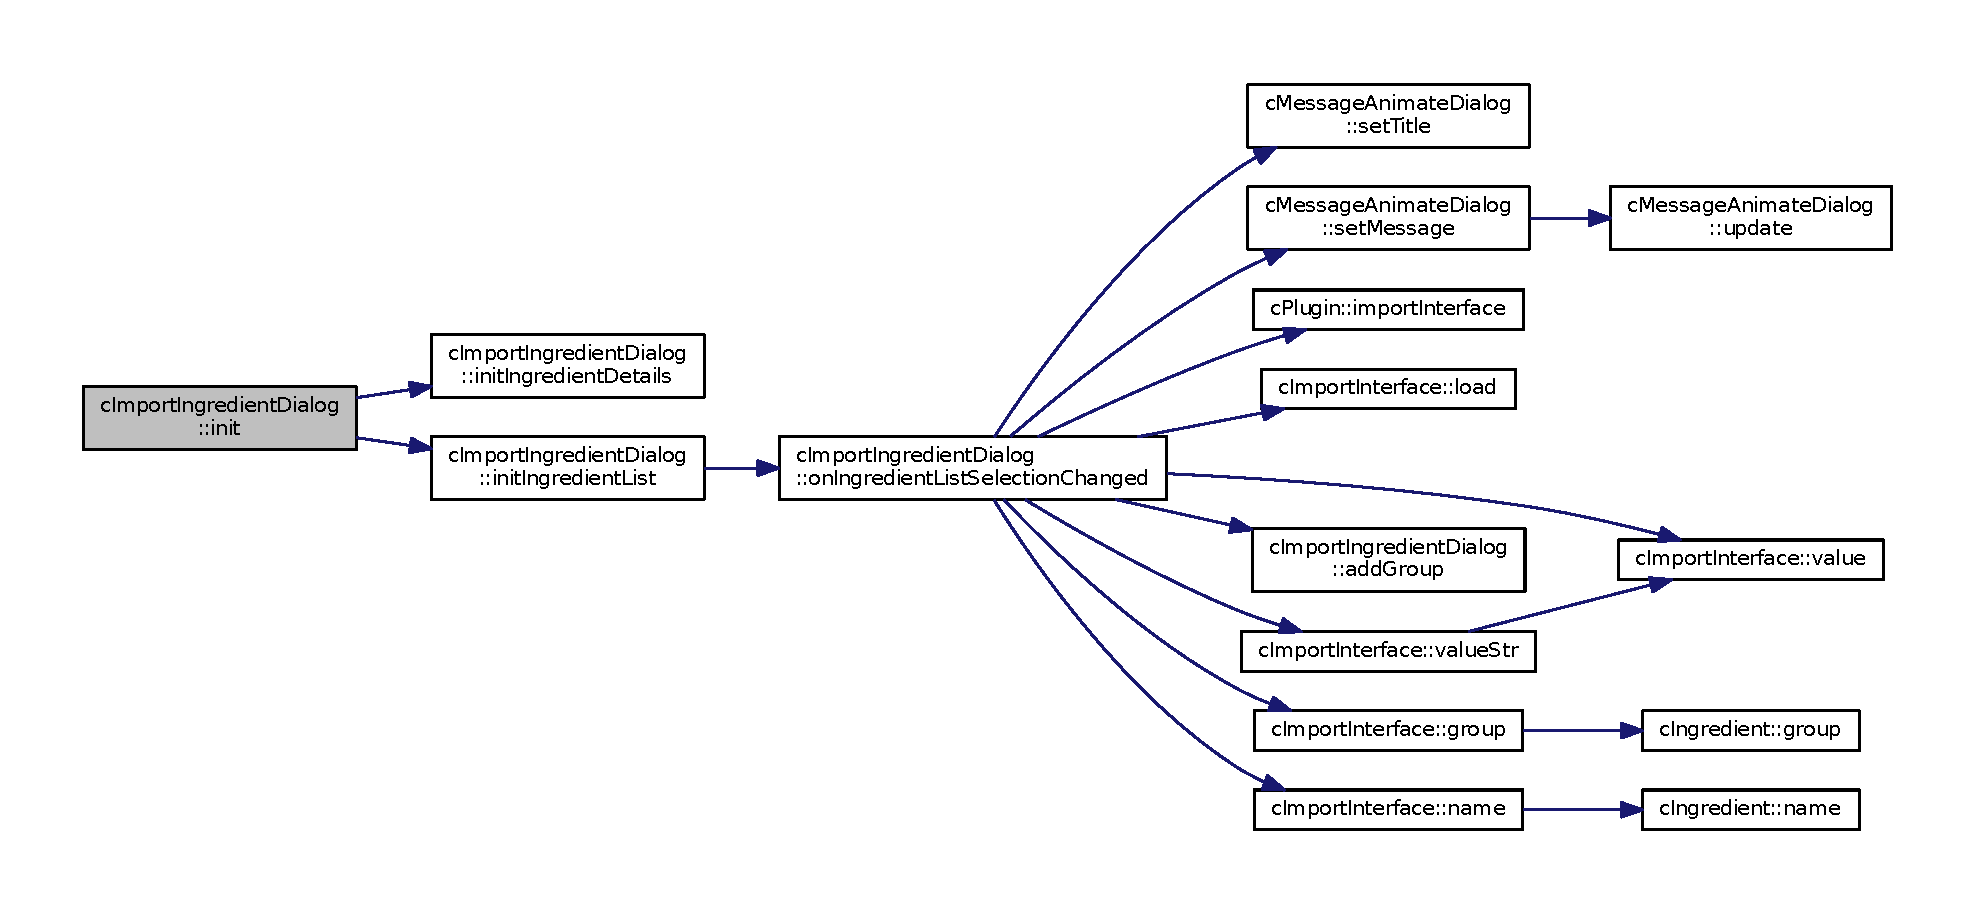
\includegraphics[width=350pt]{classc_import_ingredient_dialog_acd246954f20eba6d65d233adb3a9c293_cgraph}
\end{center}
\end{figure}




Here is the caller graph for this function\+:
\nopagebreak
\begin{figure}[H]
\begin{center}
\leavevmode
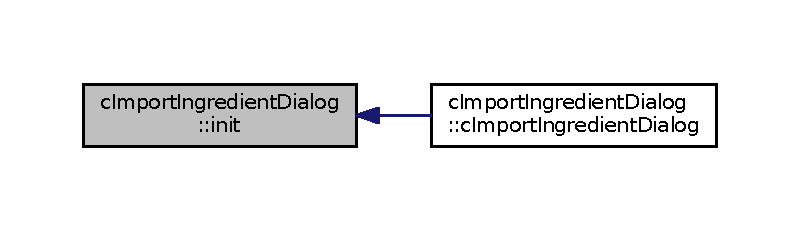
\includegraphics[width=350pt]{classc_import_ingredient_dialog_acd246954f20eba6d65d233adb3a9c293_icgraph}
\end{center}
\end{figure}


\index{c\+Import\+Ingredient\+Dialog@{c\+Import\+Ingredient\+Dialog}!init\+Ingredient\+Details@{init\+Ingredient\+Details}}
\index{init\+Ingredient\+Details@{init\+Ingredient\+Details}!c\+Import\+Ingredient\+Dialog@{c\+Import\+Ingredient\+Dialog}}
\subsubsection[{\texorpdfstring{init\+Ingredient\+Details()}{initIngredientDetails()}}]{\setlength{\rightskip}{0pt plus 5cm}void c\+Import\+Ingredient\+Dialog\+::init\+Ingredient\+Details (
\begin{DoxyParamCaption}
{}
\end{DoxyParamCaption}
)\hspace{0.3cm}{\ttfamily [protected]}}\hypertarget{classc_import_ingredient_dialog_a6158a639b7b11973e84ddb3ca7d9aeb6}{}\label{classc_import_ingredient_dialog_a6158a639b7b11973e84ddb3ca7d9aeb6}


References m\+\_\+lp\+Ingredient\+Details\+Model, and ui.



Referenced by init().



Here is the caller graph for this function\+:
\nopagebreak
\begin{figure}[H]
\begin{center}
\leavevmode
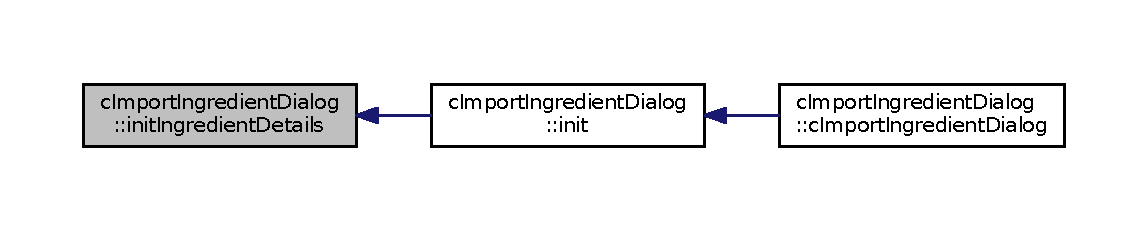
\includegraphics[width=350pt]{classc_import_ingredient_dialog_a6158a639b7b11973e84ddb3ca7d9aeb6_icgraph}
\end{center}
\end{figure}


\index{c\+Import\+Ingredient\+Dialog@{c\+Import\+Ingredient\+Dialog}!init\+Ingredient\+List@{init\+Ingredient\+List}}
\index{init\+Ingredient\+List@{init\+Ingredient\+List}!c\+Import\+Ingredient\+Dialog@{c\+Import\+Ingredient\+Dialog}}
\subsubsection[{\texorpdfstring{init\+Ingredient\+List()}{initIngredientList()}}]{\setlength{\rightskip}{0pt plus 5cm}void c\+Import\+Ingredient\+Dialog\+::init\+Ingredient\+List (
\begin{DoxyParamCaption}
{}
\end{DoxyParamCaption}
)\hspace{0.3cm}{\ttfamily [protected]}}\hypertarget{classc_import_ingredient_dialog_adf78505fef0d070021878b885fd5a0ea}{}\label{classc_import_ingredient_dialog_adf78505fef0d070021878b885fd5a0ea}


References m\+\_\+lp\+Ingredient\+List\+Model, on\+Ingredient\+List\+Selection\+Changed(), and ui.



Referenced by init().



Here is the call graph for this function\+:
\nopagebreak
\begin{figure}[H]
\begin{center}
\leavevmode
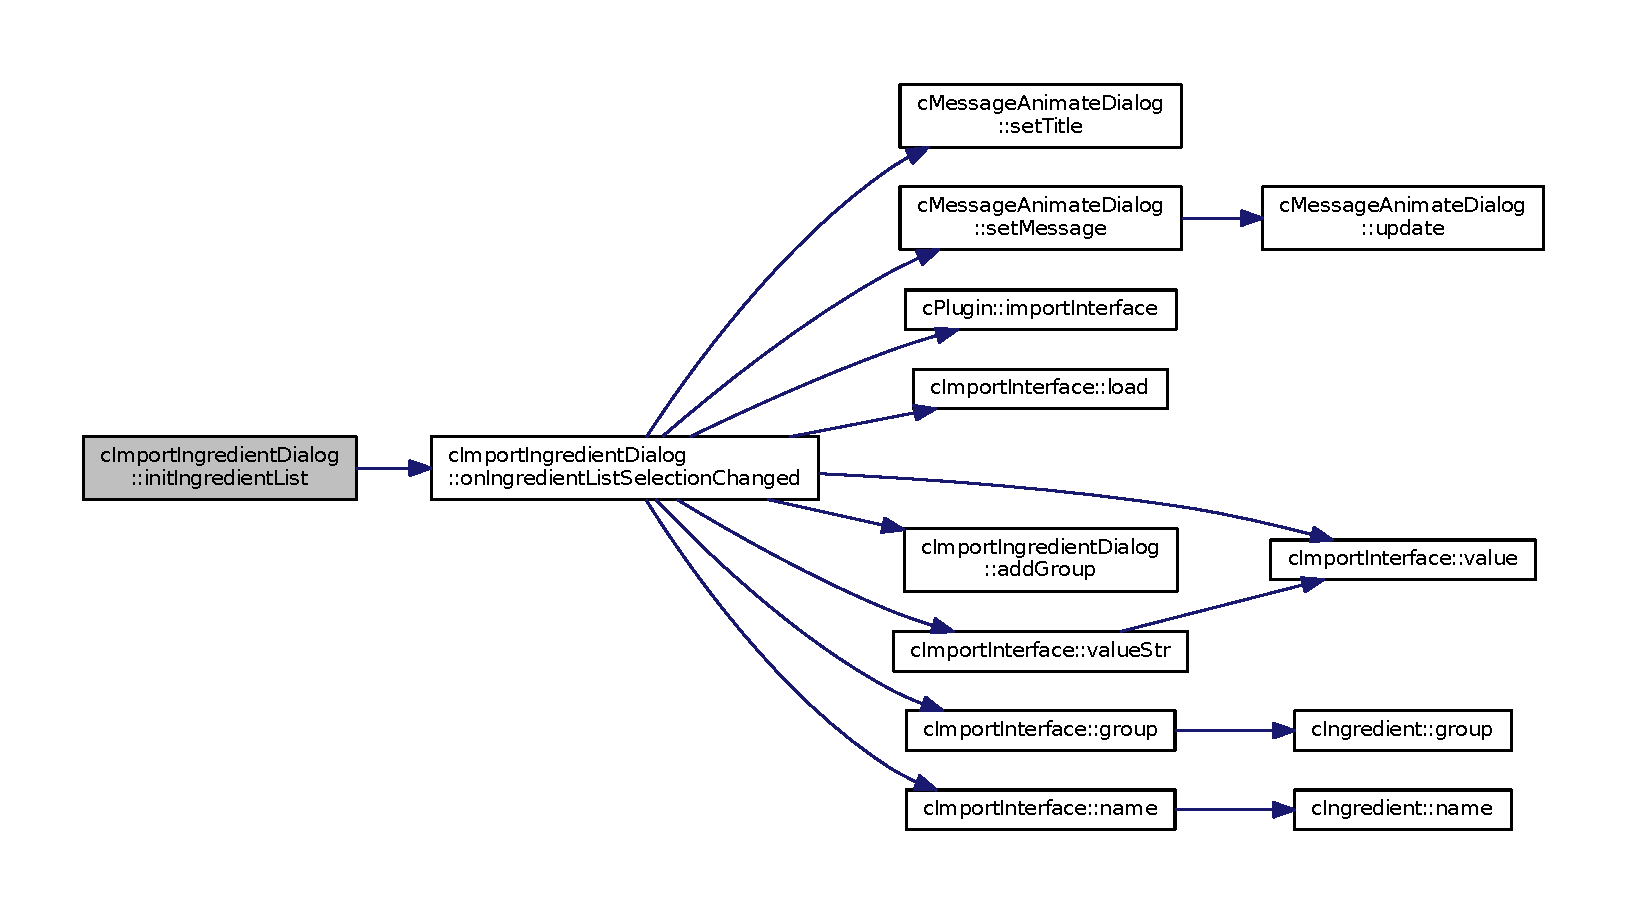
\includegraphics[width=350pt]{classc_import_ingredient_dialog_adf78505fef0d070021878b885fd5a0ea_cgraph}
\end{center}
\end{figure}




Here is the caller graph for this function\+:
\nopagebreak
\begin{figure}[H]
\begin{center}
\leavevmode
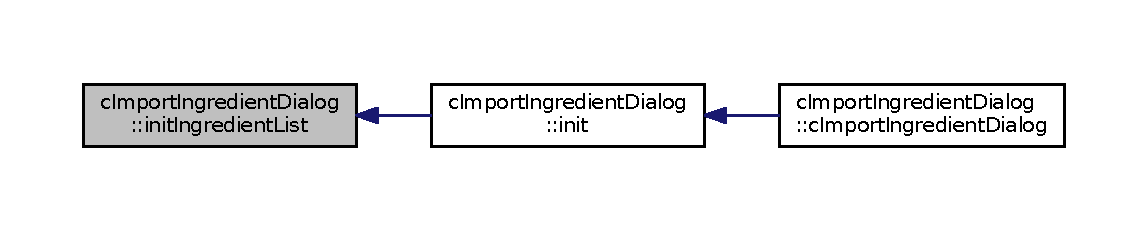
\includegraphics[width=350pt]{classc_import_ingredient_dialog_adf78505fef0d070021878b885fd5a0ea_icgraph}
\end{center}
\end{figure}


\index{c\+Import\+Ingredient\+Dialog@{c\+Import\+Ingredient\+Dialog}!on\+\_\+m\+\_\+lp\+Search\+Button\+\_\+clicked@{on\+\_\+m\+\_\+lp\+Search\+Button\+\_\+clicked}}
\index{on\+\_\+m\+\_\+lp\+Search\+Button\+\_\+clicked@{on\+\_\+m\+\_\+lp\+Search\+Button\+\_\+clicked}!c\+Import\+Ingredient\+Dialog@{c\+Import\+Ingredient\+Dialog}}
\subsubsection[{\texorpdfstring{on\+\_\+m\+\_\+lp\+Search\+Button\+\_\+clicked}{on_m_lpSearchButton_clicked}}]{\setlength{\rightskip}{0pt plus 5cm}void c\+Import\+Ingredient\+Dialog\+::on\+\_\+m\+\_\+lp\+Search\+Button\+\_\+clicked (
\begin{DoxyParamCaption}
{}
\end{DoxyParamCaption}
)\hspace{0.3cm}{\ttfamily [private]}, {\ttfamily [slot]}}\hypertarget{classc_import_ingredient_dialog_aad6f67e1420e7ceba52d6ea72bf70e88}{}\label{classc_import_ingredient_dialog_aad6f67e1420e7ceba52d6ea72bf70e88}


References c\+Plugin\+::import\+Interface(), m\+\_\+lp\+Ingredient\+List\+Model, c\+Import\+Interface\+::search(), c\+Message\+Animate\+Dialog\+::set\+Message(), c\+Message\+Animate\+Dialog\+::set\+Title(), and ui.



Here is the call graph for this function\+:
\nopagebreak
\begin{figure}[H]
\begin{center}
\leavevmode
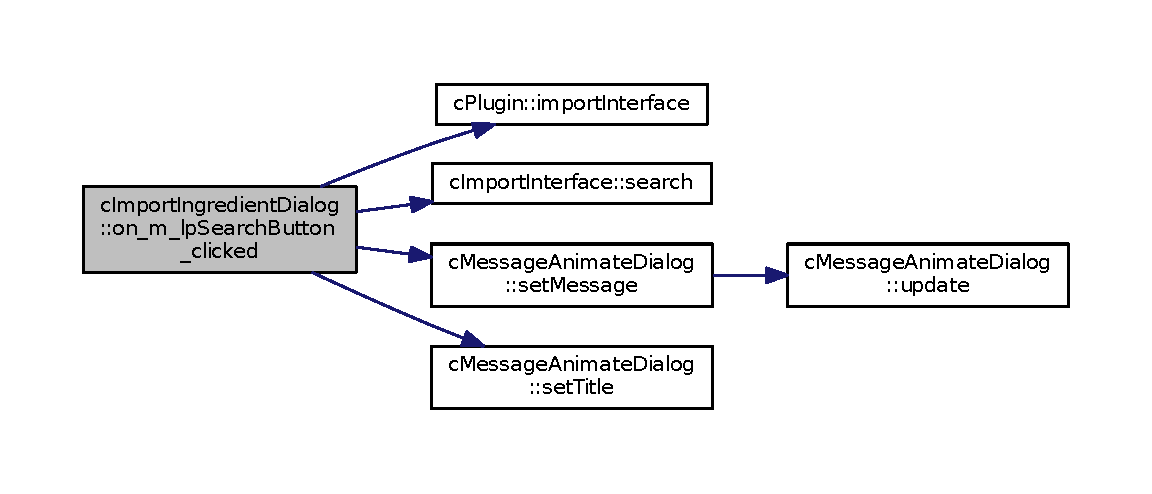
\includegraphics[width=350pt]{classc_import_ingredient_dialog_aad6f67e1420e7ceba52d6ea72bf70e88_cgraph}
\end{center}
\end{figure}


\index{c\+Import\+Ingredient\+Dialog@{c\+Import\+Ingredient\+Dialog}!on\+\_\+m\+\_\+lp\+Search\+String\+\_\+text\+Changed@{on\+\_\+m\+\_\+lp\+Search\+String\+\_\+text\+Changed}}
\index{on\+\_\+m\+\_\+lp\+Search\+String\+\_\+text\+Changed@{on\+\_\+m\+\_\+lp\+Search\+String\+\_\+text\+Changed}!c\+Import\+Ingredient\+Dialog@{c\+Import\+Ingredient\+Dialog}}
\subsubsection[{\texorpdfstring{on\+\_\+m\+\_\+lp\+Search\+String\+\_\+text\+Changed}{on_m_lpSearchString_textChanged}}]{\setlength{\rightskip}{0pt plus 5cm}void c\+Import\+Ingredient\+Dialog\+::on\+\_\+m\+\_\+lp\+Search\+String\+\_\+text\+Changed (
\begin{DoxyParamCaption}
\item[{const Q\+String \&}]{arg1}
\end{DoxyParamCaption}
)\hspace{0.3cm}{\ttfamily [private]}, {\ttfamily [slot]}}\hypertarget{classc_import_ingredient_dialog_a2b5fa289051ab3b18e71f7e2cb7573b3}{}\label{classc_import_ingredient_dialog_a2b5fa289051ab3b18e71f7e2cb7573b3}


References ui.

\index{c\+Import\+Ingredient\+Dialog@{c\+Import\+Ingredient\+Dialog}!on\+Ingredient\+List\+Selection\+Changed@{on\+Ingredient\+List\+Selection\+Changed}}
\index{on\+Ingredient\+List\+Selection\+Changed@{on\+Ingredient\+List\+Selection\+Changed}!c\+Import\+Ingredient\+Dialog@{c\+Import\+Ingredient\+Dialog}}
\subsubsection[{\texorpdfstring{on\+Ingredient\+List\+Selection\+Changed}{onIngredientListSelectionChanged}}]{\setlength{\rightskip}{0pt plus 5cm}void c\+Import\+Ingredient\+Dialog\+::on\+Ingredient\+List\+Selection\+Changed (
\begin{DoxyParamCaption}
\item[{const Q\+Item\+Selection \&}]{selected, }
\item[{const Q\+Item\+Selection \&}]{deselected}
\end{DoxyParamCaption}
)\hspace{0.3cm}{\ttfamily [private]}, {\ttfamily [slot]}}\hypertarget{classc_import_ingredient_dialog_a7aaca4be76facdc5c90fd321825a6289}{}\label{classc_import_ingredient_dialog_a7aaca4be76facdc5c90fd321825a6289}

\begin{DoxyParams}{Parameters}
{\em selected} & \\
\hline
{\em deselected} & \\
\hline
\end{DoxyParams}


References add\+Group(), c\+Import\+Interface\+::group(), c\+Ingredient\+::i\+Ingredient\+Max, c\+Plugin\+::import\+Interface(), c\+Import\+Interface\+::load(), m\+\_\+lp\+Ingredient\+Details\+Model, c\+Import\+Interface\+::name(), c\+Message\+Animate\+Dialog\+::set\+Message(), c\+Message\+Animate\+Dialog\+::set\+Title(), ui, c\+Import\+Interface\+::value(), and c\+Import\+Interface\+::value\+Str().



Referenced by init\+Ingredient\+List().



Here is the call graph for this function\+:
\nopagebreak
\begin{figure}[H]
\begin{center}
\leavevmode
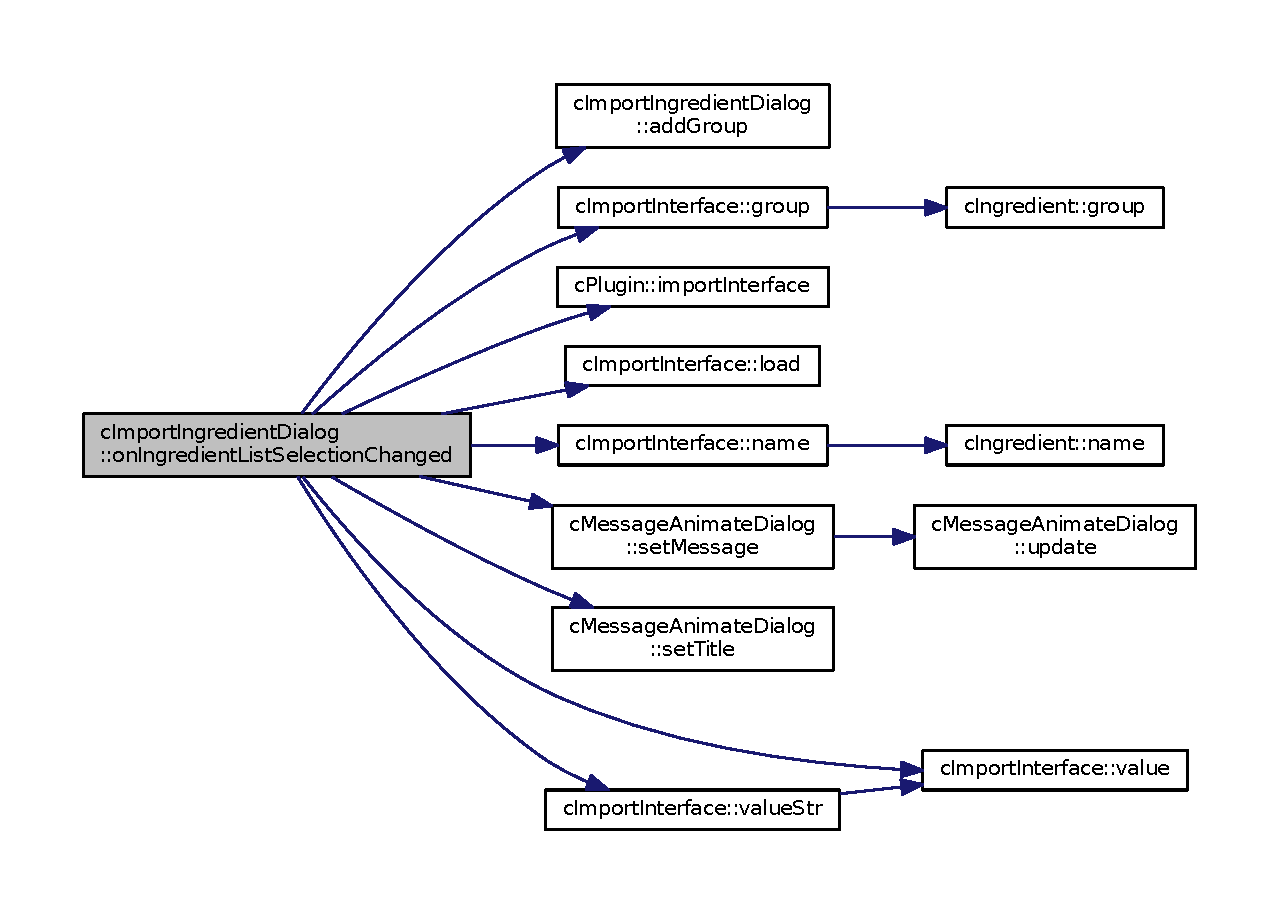
\includegraphics[width=350pt]{classc_import_ingredient_dialog_a7aaca4be76facdc5c90fd321825a6289_cgraph}
\end{center}
\end{figure}




Here is the caller graph for this function\+:
\nopagebreak
\begin{figure}[H]
\begin{center}
\leavevmode
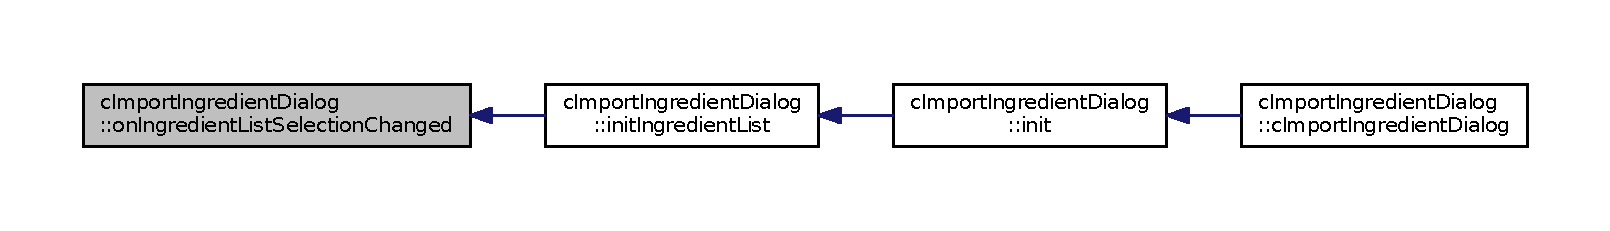
\includegraphics[width=350pt]{classc_import_ingredient_dialog_a7aaca4be76facdc5c90fd321825a6289_icgraph}
\end{center}
\end{figure}


\index{c\+Import\+Ingredient\+Dialog@{c\+Import\+Ingredient\+Dialog}!set\+Plugin\+List@{set\+Plugin\+List}}
\index{set\+Plugin\+List@{set\+Plugin\+List}!c\+Import\+Ingredient\+Dialog@{c\+Import\+Ingredient\+Dialog}}
\subsubsection[{\texorpdfstring{set\+Plugin\+List(const Q\+List$<$ c\+Plugin $\ast$ $>$ plugin\+List)}{setPluginList(const QList< cPlugin * > pluginList)}}]{\setlength{\rightskip}{0pt plus 5cm}void c\+Import\+Ingredient\+Dialog\+::set\+Plugin\+List (
\begin{DoxyParamCaption}
\item[{const Q\+List$<$ {\bf c\+Plugin} $\ast$ $>$}]{plugin\+List}
\end{DoxyParamCaption}
)}\hypertarget{classc_import_ingredient_dialog_ad710be68582d34c43a399b4764c0434a}{}\label{classc_import_ingredient_dialog_ad710be68582d34c43a399b4764c0434a}

\begin{DoxyParams}{Parameters}
{\em plugin\+List} & \\
\hline
\end{DoxyParams}


References c\+Plugin\+::capability(), m\+\_\+plugin\+List, c\+Plugin\+::\+Plugin\+Cap\+Import, c\+Plugin\+::plugin\+Name(), and ui.



Referenced by c\+Main\+Window\+::on\+Ingredients\+List\+Import().



Here is the call graph for this function\+:
\nopagebreak
\begin{figure}[H]
\begin{center}
\leavevmode
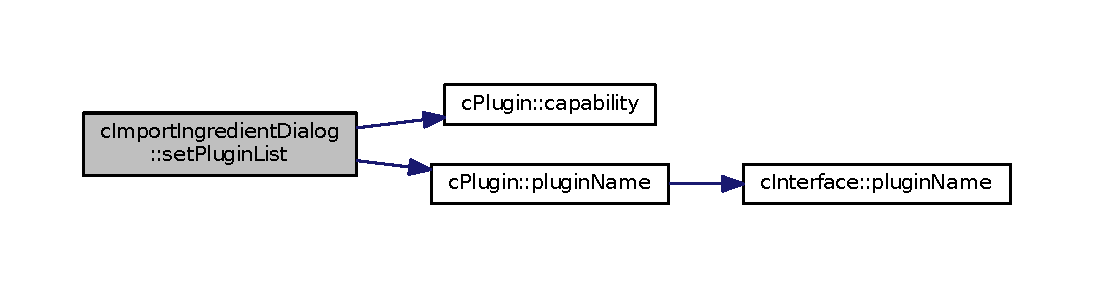
\includegraphics[width=350pt]{classc_import_ingredient_dialog_ad710be68582d34c43a399b4764c0434a_cgraph}
\end{center}
\end{figure}




Here is the caller graph for this function\+:
\nopagebreak
\begin{figure}[H]
\begin{center}
\leavevmode
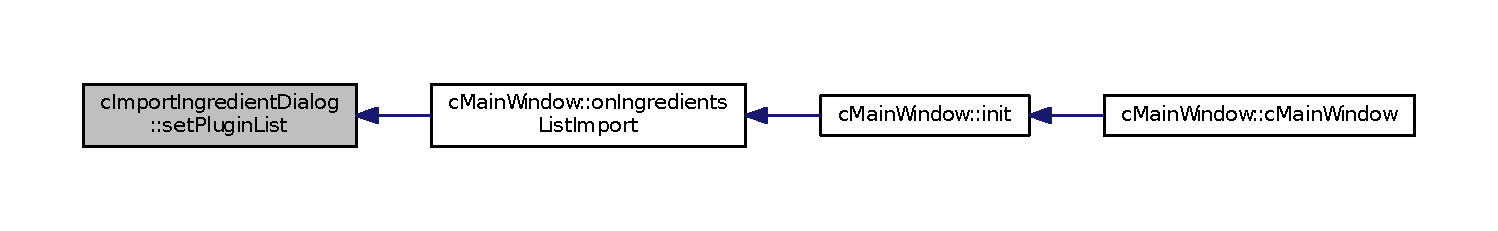
\includegraphics[width=350pt]{classc_import_ingredient_dialog_ad710be68582d34c43a399b4764c0434a_icgraph}
\end{center}
\end{figure}




\subsection{Member Data Documentation}
\index{c\+Import\+Ingredient\+Dialog@{c\+Import\+Ingredient\+Dialog}!m\+\_\+lp\+Ingredient\+Details\+Model@{m\+\_\+lp\+Ingredient\+Details\+Model}}
\index{m\+\_\+lp\+Ingredient\+Details\+Model@{m\+\_\+lp\+Ingredient\+Details\+Model}!c\+Import\+Ingredient\+Dialog@{c\+Import\+Ingredient\+Dialog}}
\subsubsection[{\texorpdfstring{m\+\_\+lp\+Ingredient\+Details\+Model}{m_lpIngredientDetailsModel}}]{\setlength{\rightskip}{0pt plus 5cm}Q\+Standard\+Item\+Model$\ast$ c\+Import\+Ingredient\+Dialog\+::m\+\_\+lp\+Ingredient\+Details\+Model\hspace{0.3cm}{\ttfamily [private]}}\hypertarget{classc_import_ingredient_dialog_a9fcdb59fa6c5fc9b65c4db1e43afb3db}{}\label{classc_import_ingredient_dialog_a9fcdb59fa6c5fc9b65c4db1e43afb3db}
T\+O\+DO\+: describe 

Referenced by add\+Group(), init\+Ingredient\+Details(), and on\+Ingredient\+List\+Selection\+Changed().

\index{c\+Import\+Ingredient\+Dialog@{c\+Import\+Ingredient\+Dialog}!m\+\_\+lp\+Ingredient\+List\+Model@{m\+\_\+lp\+Ingredient\+List\+Model}}
\index{m\+\_\+lp\+Ingredient\+List\+Model@{m\+\_\+lp\+Ingredient\+List\+Model}!c\+Import\+Ingredient\+Dialog@{c\+Import\+Ingredient\+Dialog}}
\subsubsection[{\texorpdfstring{m\+\_\+lp\+Ingredient\+List\+Model}{m_lpIngredientListModel}}]{\setlength{\rightskip}{0pt plus 5cm}Q\+Standard\+Item\+Model$\ast$ c\+Import\+Ingredient\+Dialog\+::m\+\_\+lp\+Ingredient\+List\+Model\hspace{0.3cm}{\ttfamily [private]}}\hypertarget{classc_import_ingredient_dialog_a0fe1def4e950a1f06a14f28ff7d9ba6a}{}\label{classc_import_ingredient_dialog_a0fe1def4e950a1f06a14f28ff7d9ba6a}
T\+O\+DO\+: describe 

Referenced by init\+Ingredient\+List(), and on\+\_\+m\+\_\+lp\+Search\+Button\+\_\+clicked().

\index{c\+Import\+Ingredient\+Dialog@{c\+Import\+Ingredient\+Dialog}!m\+\_\+plugin\+List@{m\+\_\+plugin\+List}}
\index{m\+\_\+plugin\+List@{m\+\_\+plugin\+List}!c\+Import\+Ingredient\+Dialog@{c\+Import\+Ingredient\+Dialog}}
\subsubsection[{\texorpdfstring{m\+\_\+plugin\+List}{m_pluginList}}]{\setlength{\rightskip}{0pt plus 5cm}Q\+List$<${\bf c\+Plugin}$\ast$$>$ c\+Import\+Ingredient\+Dialog\+::m\+\_\+plugin\+List\hspace{0.3cm}{\ttfamily [protected]}}\hypertarget{classc_import_ingredient_dialog_ad5795b238430db474ae852bfbb493578}{}\label{classc_import_ingredient_dialog_ad5795b238430db474ae852bfbb493578}
T\+O\+DO\+: describe 

Referenced by set\+Plugin\+List().

\index{c\+Import\+Ingredient\+Dialog@{c\+Import\+Ingredient\+Dialog}!ui@{ui}}
\index{ui@{ui}!c\+Import\+Ingredient\+Dialog@{c\+Import\+Ingredient\+Dialog}}
\subsubsection[{\texorpdfstring{ui}{ui}}]{\setlength{\rightskip}{0pt plus 5cm}Ui\+::c\+Import\+Ingredient\+Dialog$\ast$ c\+Import\+Ingredient\+Dialog\+::ui\hspace{0.3cm}{\ttfamily [private]}}\hypertarget{classc_import_ingredient_dialog_a80da8aa411eb8da3a692693445e64408}{}\label{classc_import_ingredient_dialog_a80da8aa411eb8da3a692693445e64408}
T\+O\+DO\+: describe 

Referenced by init(), init\+Ingredient\+Details(), init\+Ingredient\+List(), on\+\_\+m\+\_\+lp\+Search\+Button\+\_\+clicked(), on\+\_\+m\+\_\+lp\+Search\+String\+\_\+text\+Changed(), on\+Ingredient\+List\+Selection\+Changed(), set\+Plugin\+List(), and $\sim$c\+Import\+Ingredient\+Dialog().



The documentation for this class was generated from the following files\+:\begin{DoxyCompactItemize}
\item 
Kooky/\hyperlink{cimportingredientdialog_8h}{cimportingredientdialog.\+h}\item 
Kooky/\hyperlink{cimportingredientdialog_8cpp}{cimportingredientdialog.\+cpp}\end{DoxyCompactItemize}

\hypertarget{classc_import_interface}{}\section{c\+Import\+Interface Class Reference}
\label{classc_import_interface}\index{c\+Import\+Interface@{c\+Import\+Interface}}


Interface class for importing data.  




{\ttfamily \#include $<$cimportinterface.\+h$>$}



Inheritance diagram for c\+Import\+Interface\+:
\nopagebreak
\begin{figure}[H]
\begin{center}
\leavevmode
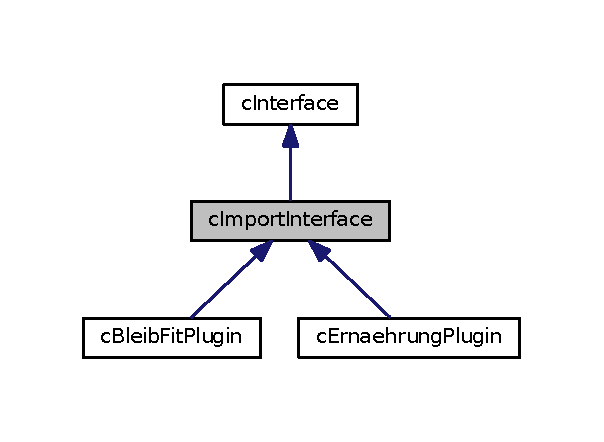
\includegraphics[width=290pt]{classc_import_interface__inherit__graph}
\end{center}
\end{figure}


Collaboration diagram for c\+Import\+Interface\+:
\nopagebreak
\begin{figure}[H]
\begin{center}
\leavevmode
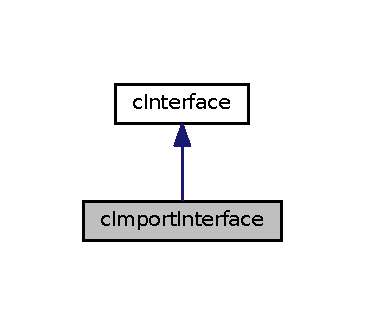
\includegraphics[width=175pt]{classc_import_interface__coll__graph}
\end{center}
\end{figure}
\subsection*{Public Member Functions}
\begin{DoxyCompactItemize}
\item 
\hyperlink{classc_import_interface_a66f54591d75e8aa458e5afb91b3f3177}{c\+Import\+Interface} ()
\item 
virtual Q\+Map$<$ Q\+String, Q\+String $>$ \hyperlink{classc_import_interface_a4ec2f198f8488e7daf2e93cf637a580d}{details\+Capability} ()=0
\item 
virtual Q\+String\+List \hyperlink{classc_import_interface_a8b48a3821674ff15d7eaf4e03c55409f}{search} (const Q\+String \&sz\+Search, const Q\+String \&sz\+Details=Q\+String(\char`\"{}\char`\"{}))=0
\item 
virtual bool \hyperlink{classc_import_interface_a728bcb2a636f78bae2fe7e128a18e983}{load} (qint16 i\+Index)=0
\item 
bool \hyperlink{classc_import_interface_a898e0fc3651bbf855ee28756e69d48fb}{loaded} ()
\item 
virtual qreal \hyperlink{classc_import_interface_a7a8dbe6a164549272d748d2f77aebc42}{value} (\hyperlink{classc_ingredient_acf023723841ec66cd6368a25e3174a28}{c\+Ingredient\+::i\+Ingredient} i)=0
\item 
Q\+String \hyperlink{classc_import_interface_a272c43d684b605f36d36cb20e4039d94}{value\+Str} (\hyperlink{classc_ingredient_acf023723841ec66cd6368a25e3174a28}{c\+Ingredient\+::i\+Ingredient} i)
\item 
Q\+String \hyperlink{classc_import_interface_a685fafcac4d7194045e6c9e2d84d7981}{name} (\hyperlink{classc_ingredient_acf023723841ec66cd6368a25e3174a28}{c\+Ingredient\+::i\+Ingredient} i)
\item 
Q\+String \hyperlink{classc_import_interface_a1d31c90d6ef27a2b9edfb99e655120ea}{group} (\hyperlink{classc_ingredient_acf023723841ec66cd6368a25e3174a28}{c\+Ingredient\+::i\+Ingredient} i)
\item 
virtual Q\+String \hyperlink{classc_import_interface_af3f569b605787021a919816978f229bc}{ingredient\+Name} ()=0
\end{DoxyCompactItemize}
\subsection*{Protected Attributes}
\begin{DoxyCompactItemize}
\item 
bool \hyperlink{classc_import_interface_ae58ec0e6b990aa6624a12af9dc20e8dc}{m\+\_\+b\+Loaded}
\item 
qint16 \hyperlink{classc_import_interface_ab18dd3e9cf49a07f23f376362fdf317b}{m\+\_\+i\+Loaded\+Index}
\end{DoxyCompactItemize}
\subsection*{Additional Inherited Members}


\subsection{Detailed Description}
This class implements basic import functionality for Kooky. All functions may be overwritten by derriving classes.

\begin{DoxyNote}{Note}
Attempts at zen rarely work.
\end{DoxyNote}
\begin{DoxyAuthor}{Author}
Herwig Birke
\end{DoxyAuthor}
\begin{DoxyVersion}{Version}
1.\+0
\end{DoxyVersion}
\begin{DoxyDate}{Date}
\$\+Date\+: 2016/02/09 
\end{DoxyDate}


\subsection{Constructor \& Destructor Documentation}
\index{c\+Import\+Interface@{c\+Import\+Interface}!c\+Import\+Interface@{c\+Import\+Interface}}
\index{c\+Import\+Interface@{c\+Import\+Interface}!c\+Import\+Interface@{c\+Import\+Interface}}
\subsubsection[{\texorpdfstring{c\+Import\+Interface()}{cImportInterface()}}]{\setlength{\rightskip}{0pt plus 5cm}c\+Import\+Interface\+::c\+Import\+Interface (
\begin{DoxyParamCaption}
{}
\end{DoxyParamCaption}
)\hspace{0.3cm}{\ttfamily [inline]}}\hypertarget{classc_import_interface_a66f54591d75e8aa458e5afb91b3f3177}{}\label{classc_import_interface_a66f54591d75e8aa458e5afb91b3f3177}


References details\+Capability(), load(), and search().



Here is the call graph for this function\+:
\nopagebreak
\begin{figure}[H]
\begin{center}
\leavevmode
\includegraphics[width=350pt]{classc_import_interface_a66f54591d75e8aa458e5afb91b3f3177_cgraph}
\end{center}
\end{figure}




\subsection{Member Function Documentation}
\index{c\+Import\+Interface@{c\+Import\+Interface}!details\+Capability@{details\+Capability}}
\index{details\+Capability@{details\+Capability}!c\+Import\+Interface@{c\+Import\+Interface}}
\subsubsection[{\texorpdfstring{details\+Capability()=0}{detailsCapability()=0}}]{\setlength{\rightskip}{0pt plus 5cm}virtual Q\+Map$<$Q\+String, Q\+String$>$ c\+Import\+Interface\+::details\+Capability (
\begin{DoxyParamCaption}
{}
\end{DoxyParamCaption}
)\hspace{0.3cm}{\ttfamily [pure virtual]}}\hypertarget{classc_import_interface_a4ec2f198f8488e7daf2e93cf637a580d}{}\label{classc_import_interface_a4ec2f198f8488e7daf2e93cf637a580d}
\begin{DoxyReturn}{Returns}
Q\+Map$<$\+Q\+String, Q\+String$>$ 
\end{DoxyReturn}


Implemented in \hyperlink{classc_bleib_fit_plugin_af3db6c6ff6bb28787d67e4cc3e957e90}{c\+Bleib\+Fit\+Plugin}, and \hyperlink{classc_ernaehrung_plugin_a9fef4cc5e1c59999833ffb4493cfae3e}{c\+Ernaehrung\+Plugin}.



Referenced by c\+Import\+Interface().



Here is the caller graph for this function\+:
\nopagebreak
\begin{figure}[H]
\begin{center}
\leavevmode
\includegraphics[width=350pt]{classc_import_interface_a4ec2f198f8488e7daf2e93cf637a580d_icgraph}
\end{center}
\end{figure}


\index{c\+Import\+Interface@{c\+Import\+Interface}!group@{group}}
\index{group@{group}!c\+Import\+Interface@{c\+Import\+Interface}}
\subsubsection[{\texorpdfstring{group(c\+Ingredient\+::i\+Ingredient i)}{group(cIngredient::iIngredient i)}}]{\setlength{\rightskip}{0pt plus 5cm}Q\+String c\+Import\+Interface\+::group (
\begin{DoxyParamCaption}
\item[{{\bf c\+Ingredient\+::i\+Ingredient}}]{i}
\end{DoxyParamCaption}
)}\hypertarget{classc_import_interface_a1d31c90d6ef27a2b9edfb99e655120ea}{}\label{classc_import_interface_a1d31c90d6ef27a2b9edfb99e655120ea}

\begin{DoxyParams}{Parameters}
{\em i} & \\
\hline
\end{DoxyParams}
\begin{DoxyReturn}{Returns}
Q\+String 
\end{DoxyReturn}


References c\+Ingredient\+::group().



Referenced by loaded(), and c\+Import\+Ingredient\+Dialog\+::on\+Ingredient\+List\+Selection\+Changed().



Here is the call graph for this function\+:
\nopagebreak
\begin{figure}[H]
\begin{center}
\leavevmode
\includegraphics[width=349pt]{classc_import_interface_a1d31c90d6ef27a2b9edfb99e655120ea_cgraph}
\end{center}
\end{figure}




Here is the caller graph for this function\+:
\nopagebreak
\begin{figure}[H]
\begin{center}
\leavevmode
\includegraphics[width=350pt]{classc_import_interface_a1d31c90d6ef27a2b9edfb99e655120ea_icgraph}
\end{center}
\end{figure}


\index{c\+Import\+Interface@{c\+Import\+Interface}!ingredient\+Name@{ingredient\+Name}}
\index{ingredient\+Name@{ingredient\+Name}!c\+Import\+Interface@{c\+Import\+Interface}}
\subsubsection[{\texorpdfstring{ingredient\+Name()=0}{ingredientName()=0}}]{\setlength{\rightskip}{0pt plus 5cm}virtual Q\+String c\+Import\+Interface\+::ingredient\+Name (
\begin{DoxyParamCaption}
{}
\end{DoxyParamCaption}
)\hspace{0.3cm}{\ttfamily [pure virtual]}}\hypertarget{classc_import_interface_af3f569b605787021a919816978f229bc}{}\label{classc_import_interface_af3f569b605787021a919816978f229bc}
\begin{DoxyReturn}{Returns}
Q\+String 
\end{DoxyReturn}


Implemented in \hyperlink{classc_bleib_fit_plugin_a67b808ffb0884950a8652cc72e8b2d80}{c\+Bleib\+Fit\+Plugin}, and \hyperlink{classc_ernaehrung_plugin_a24c04c0b98fb4186e5b5b012662b39ed}{c\+Ernaehrung\+Plugin}.



Referenced by loaded().



Here is the caller graph for this function\+:
\nopagebreak
\begin{figure}[H]
\begin{center}
\leavevmode
\includegraphics[width=350pt]{classc_import_interface_af3f569b605787021a919816978f229bc_icgraph}
\end{center}
\end{figure}


\index{c\+Import\+Interface@{c\+Import\+Interface}!load@{load}}
\index{load@{load}!c\+Import\+Interface@{c\+Import\+Interface}}
\subsubsection[{\texorpdfstring{load(qint16 i\+Index)=0}{load(qint16 iIndex)=0}}]{\setlength{\rightskip}{0pt plus 5cm}virtual bool c\+Import\+Interface\+::load (
\begin{DoxyParamCaption}
\item[{qint16}]{i\+Index}
\end{DoxyParamCaption}
)\hspace{0.3cm}{\ttfamily [pure virtual]}}\hypertarget{classc_import_interface_a728bcb2a636f78bae2fe7e128a18e983}{}\label{classc_import_interface_a728bcb2a636f78bae2fe7e128a18e983}

\begin{DoxyParams}{Parameters}
{\em i\+Index} & \\
\hline
\end{DoxyParams}
\begin{DoxyReturn}{Returns}
bool 
\end{DoxyReturn}


Implemented in \hyperlink{classc_bleib_fit_plugin_a15e5627fa41d2f079a96267e559fccee}{c\+Bleib\+Fit\+Plugin}, and \hyperlink{classc_ernaehrung_plugin_a2d688c0a56bed5b8f233dd5890a96a3d}{c\+Ernaehrung\+Plugin}.



Referenced by c\+Import\+Interface(), and c\+Import\+Ingredient\+Dialog\+::on\+Ingredient\+List\+Selection\+Changed().



Here is the caller graph for this function\+:
\nopagebreak
\begin{figure}[H]
\begin{center}
\leavevmode
\includegraphics[width=350pt]{classc_import_interface_a728bcb2a636f78bae2fe7e128a18e983_icgraph}
\end{center}
\end{figure}


\index{c\+Import\+Interface@{c\+Import\+Interface}!loaded@{loaded}}
\index{loaded@{loaded}!c\+Import\+Interface@{c\+Import\+Interface}}
\subsubsection[{\texorpdfstring{loaded()}{loaded()}}]{\setlength{\rightskip}{0pt plus 5cm}bool c\+Import\+Interface\+::loaded (
\begin{DoxyParamCaption}
{}
\end{DoxyParamCaption}
)\hspace{0.3cm}{\ttfamily [inline]}}\hypertarget{classc_import_interface_a898e0fc3651bbf855ee28756e69d48fb}{}\label{classc_import_interface_a898e0fc3651bbf855ee28756e69d48fb}
\begin{DoxyReturn}{Returns}
bool 
\end{DoxyReturn}


References group(), ingredient\+Name(), m\+\_\+b\+Loaded, name(), value(), and value\+Str().



Here is the call graph for this function\+:
\nopagebreak
\begin{figure}[H]
\begin{center}
\leavevmode
\includegraphics[width=350pt]{classc_import_interface_a898e0fc3651bbf855ee28756e69d48fb_cgraph}
\end{center}
\end{figure}


\index{c\+Import\+Interface@{c\+Import\+Interface}!name@{name}}
\index{name@{name}!c\+Import\+Interface@{c\+Import\+Interface}}
\subsubsection[{\texorpdfstring{name(c\+Ingredient\+::i\+Ingredient i)}{name(cIngredient::iIngredient i)}}]{\setlength{\rightskip}{0pt plus 5cm}Q\+String c\+Import\+Interface\+::name (
\begin{DoxyParamCaption}
\item[{{\bf c\+Ingredient\+::i\+Ingredient}}]{i}
\end{DoxyParamCaption}
)}\hypertarget{classc_import_interface_a685fafcac4d7194045e6c9e2d84d7981}{}\label{classc_import_interface_a685fafcac4d7194045e6c9e2d84d7981}

\begin{DoxyParams}{Parameters}
{\em i} & \\
\hline
\end{DoxyParams}
\begin{DoxyReturn}{Returns}
Q\+String 
\end{DoxyReturn}


References c\+Ingredient\+::name().



Referenced by loaded(), and c\+Import\+Ingredient\+Dialog\+::on\+Ingredient\+List\+Selection\+Changed().



Here is the call graph for this function\+:
\nopagebreak
\begin{figure}[H]
\begin{center}
\leavevmode
\includegraphics[width=349pt]{classc_import_interface_a685fafcac4d7194045e6c9e2d84d7981_cgraph}
\end{center}
\end{figure}




Here is the caller graph for this function\+:
\nopagebreak
\begin{figure}[H]
\begin{center}
\leavevmode
\includegraphics[width=350pt]{classc_import_interface_a685fafcac4d7194045e6c9e2d84d7981_icgraph}
\end{center}
\end{figure}


\index{c\+Import\+Interface@{c\+Import\+Interface}!search@{search}}
\index{search@{search}!c\+Import\+Interface@{c\+Import\+Interface}}
\subsubsection[{\texorpdfstring{search(const Q\+String \&sz\+Search, const Q\+String \&sz\+Details=\+Q\+String(""""))=0}{search(const QString &szSearch, const QString &szDetails=QString(""))=0}}]{\setlength{\rightskip}{0pt plus 5cm}virtual Q\+String\+List c\+Import\+Interface\+::search (
\begin{DoxyParamCaption}
\item[{const Q\+String \&}]{sz\+Search, }
\item[{const Q\+String \&}]{sz\+Details = {\ttfamily QString(\char`\"{}\char`\"{})}}
\end{DoxyParamCaption}
)\hspace{0.3cm}{\ttfamily [pure virtual]}}\hypertarget{classc_import_interface_a8b48a3821674ff15d7eaf4e03c55409f}{}\label{classc_import_interface_a8b48a3821674ff15d7eaf4e03c55409f}

\begin{DoxyParams}{Parameters}
{\em sz\+Search} & \\
\hline
{\em sz\+Details} & \\
\hline
\end{DoxyParams}
\begin{DoxyReturn}{Returns}
Q\+String\+List 
\end{DoxyReturn}


Implemented in \hyperlink{classc_bleib_fit_plugin_a71d3dc9fc52a807e33608f2522c1ca31}{c\+Bleib\+Fit\+Plugin}, and \hyperlink{classc_ernaehrung_plugin_aec19c86cca48415dbef841bc5b3cc15d}{c\+Ernaehrung\+Plugin}.



Referenced by c\+Import\+Interface(), and c\+Import\+Ingredient\+Dialog\+::on\+\_\+m\+\_\+lp\+Search\+Button\+\_\+clicked().



Here is the caller graph for this function\+:
\nopagebreak
\begin{figure}[H]
\begin{center}
\leavevmode
\includegraphics[width=350pt]{classc_import_interface_a8b48a3821674ff15d7eaf4e03c55409f_icgraph}
\end{center}
\end{figure}


\index{c\+Import\+Interface@{c\+Import\+Interface}!value@{value}}
\index{value@{value}!c\+Import\+Interface@{c\+Import\+Interface}}
\subsubsection[{\texorpdfstring{value(c\+Ingredient\+::i\+Ingredient i)=0}{value(cIngredient::iIngredient i)=0}}]{\setlength{\rightskip}{0pt plus 5cm}virtual qreal c\+Import\+Interface\+::value (
\begin{DoxyParamCaption}
\item[{{\bf c\+Ingredient\+::i\+Ingredient}}]{i}
\end{DoxyParamCaption}
)\hspace{0.3cm}{\ttfamily [pure virtual]}}\hypertarget{classc_import_interface_a7a8dbe6a164549272d748d2f77aebc42}{}\label{classc_import_interface_a7a8dbe6a164549272d748d2f77aebc42}

\begin{DoxyParams}{Parameters}
{\em i} & \\
\hline
\end{DoxyParams}
\begin{DoxyReturn}{Returns}
qreal 
\end{DoxyReturn}


Implemented in \hyperlink{classc_bleib_fit_plugin_adb3cc6882c32a04d6d9f31961f0b8dca}{c\+Bleib\+Fit\+Plugin}, and \hyperlink{classc_ernaehrung_plugin_a8b4bb34247562c26687bb33e6369eb25}{c\+Ernaehrung\+Plugin}.



Referenced by loaded(), c\+Import\+Ingredient\+Dialog\+::on\+Ingredient\+List\+Selection\+Changed(), and value\+Str().



Here is the caller graph for this function\+:
\nopagebreak
\begin{figure}[H]
\begin{center}
\leavevmode
\includegraphics[width=350pt]{classc_import_interface_a7a8dbe6a164549272d748d2f77aebc42_icgraph}
\end{center}
\end{figure}


\index{c\+Import\+Interface@{c\+Import\+Interface}!value\+Str@{value\+Str}}
\index{value\+Str@{value\+Str}!c\+Import\+Interface@{c\+Import\+Interface}}
\subsubsection[{\texorpdfstring{value\+Str(c\+Ingredient\+::i\+Ingredient i)}{valueStr(cIngredient::iIngredient i)}}]{\setlength{\rightskip}{0pt plus 5cm}Q\+String c\+Import\+Interface\+::value\+Str (
\begin{DoxyParamCaption}
\item[{{\bf c\+Ingredient\+::i\+Ingredient}}]{i}
\end{DoxyParamCaption}
)}\hypertarget{classc_import_interface_a272c43d684b605f36d36cb20e4039d94}{}\label{classc_import_interface_a272c43d684b605f36d36cb20e4039d94}

\begin{DoxyParams}{Parameters}
{\em i} & \\
\hline
\end{DoxyParams}
\begin{DoxyReturn}{Returns}
qreal 
\end{DoxyReturn}


References c\+Ingredient\+::i\+Ingredient\+Calories, c\+Ingredient\+::i\+Ingredient\+Joule, and value().



Referenced by loaded(), and c\+Import\+Ingredient\+Dialog\+::on\+Ingredient\+List\+Selection\+Changed().



Here is the call graph for this function\+:
\nopagebreak
\begin{figure}[H]
\begin{center}
\leavevmode
\includegraphics[width=350pt]{classc_import_interface_a272c43d684b605f36d36cb20e4039d94_cgraph}
\end{center}
\end{figure}




Here is the caller graph for this function\+:
\nopagebreak
\begin{figure}[H]
\begin{center}
\leavevmode
\includegraphics[width=350pt]{classc_import_interface_a272c43d684b605f36d36cb20e4039d94_icgraph}
\end{center}
\end{figure}




\subsection{Member Data Documentation}
\index{c\+Import\+Interface@{c\+Import\+Interface}!m\+\_\+b\+Loaded@{m\+\_\+b\+Loaded}}
\index{m\+\_\+b\+Loaded@{m\+\_\+b\+Loaded}!c\+Import\+Interface@{c\+Import\+Interface}}
\subsubsection[{\texorpdfstring{m\+\_\+b\+Loaded}{m_bLoaded}}]{\setlength{\rightskip}{0pt plus 5cm}bool c\+Import\+Interface\+::m\+\_\+b\+Loaded\hspace{0.3cm}{\ttfamily [protected]}}\hypertarget{classc_import_interface_ae58ec0e6b990aa6624a12af9dc20e8dc}{}\label{classc_import_interface_ae58ec0e6b990aa6624a12af9dc20e8dc}
T\+O\+DO\+: describe 

Referenced by loaded().

\index{c\+Import\+Interface@{c\+Import\+Interface}!m\+\_\+i\+Loaded\+Index@{m\+\_\+i\+Loaded\+Index}}
\index{m\+\_\+i\+Loaded\+Index@{m\+\_\+i\+Loaded\+Index}!c\+Import\+Interface@{c\+Import\+Interface}}
\subsubsection[{\texorpdfstring{m\+\_\+i\+Loaded\+Index}{m_iLoadedIndex}}]{\setlength{\rightskip}{0pt plus 5cm}qint16 c\+Import\+Interface\+::m\+\_\+i\+Loaded\+Index\hspace{0.3cm}{\ttfamily [protected]}}\hypertarget{classc_import_interface_ab18dd3e9cf49a07f23f376362fdf317b}{}\label{classc_import_interface_ab18dd3e9cf49a07f23f376362fdf317b}
T\+O\+DO\+: describe 

The documentation for this class was generated from the following files\+:\begin{DoxyCompactItemize}
\item 
Kooky/\hyperlink{cimportinterface_8h}{cimportinterface.\+h}\item 
Kooky/\hyperlink{cimportinterface_8cpp}{cimportinterface.\+cpp}\end{DoxyCompactItemize}

\hypertarget{classc_ingredient}{}\section{c\+Ingredient Class Reference}
\label{classc_ingredient}\index{c\+Ingredient@{c\+Ingredient}}


This class holds data of an ingredient.  




{\ttfamily \#include $<$cingredient.\+h$>$}

\subsection*{Public Types}
\begin{DoxyCompactItemize}
\item 
enum \hyperlink{classc_ingredient_acf023723841ec66cd6368a25e3174a28}{i\+Ingredient} \{ \\*
\hyperlink{classc_ingredient_acf023723841ec66cd6368a25e3174a28ab889d4026db11760a8e057c915273a53}{i\+Ingredient\+Bread\+Units} = 0, 
\hyperlink{classc_ingredient_acf023723841ec66cd6368a25e3174a28a910139fbdcbe825cbd17ab1f8d98bda1}{i\+Ingredient\+Calories} = 1, 
\hyperlink{classc_ingredient_acf023723841ec66cd6368a25e3174a28ac3f49bc5d113ba83ea943fe3a31265f7}{i\+Ingredient\+Protein} = 2, 
\hyperlink{classc_ingredient_acf023723841ec66cd6368a25e3174a28a9a2354be9de0652de3c6bb1ae7a33a93}{i\+Ingredient\+Fat} = 3, 
\\*
\hyperlink{classc_ingredient_acf023723841ec66cd6368a25e3174a28a35bb83890a3eb685973a8707315508df}{i\+Ingredient\+Carbohydrates} = 4, 
\hyperlink{classc_ingredient_acf023723841ec66cd6368a25e3174a28afcb5c053eb33e8e56a5b3bf127532647}{i\+Ingredient\+Alcohol} = 5, 
\hyperlink{classc_ingredient_acf023723841ec66cd6368a25e3174a28a0f72bda1254d2141e405950d9dcade7b}{i\+Ingredient\+Water} = 6, 
\hyperlink{classc_ingredient_acf023723841ec66cd6368a25e3174a28af59a88854cae0b1af5fcd2b570d2dd13}{i\+Ingredient\+Total\+Dietary\+Fibre} = 7, 
\\*
\hyperlink{classc_ingredient_acf023723841ec66cd6368a25e3174a28a7ec96f96b0f551c1d230179b25616049}{i\+Ingredient\+Cholesterol} = 8, 
\hyperlink{classc_ingredient_acf023723841ec66cd6368a25e3174a28a76a0f875f665179f0fd36721e9efddbd}{i\+Ingredient\+Mineral} = 9, 
\hyperlink{classc_ingredient_acf023723841ec66cd6368a25e3174a28a4b16ea58a637ce7b240ab9ad8b6d68a7}{i\+Ingredient\+Vitamin\+A\+Retinol} = 10, 
\hyperlink{classc_ingredient_acf023723841ec66cd6368a25e3174a28a70b8df3c383ad6e9e061bef56c83f8c8}{i\+Ingredient\+VitaminD} = 11, 
\\*
\hyperlink{classc_ingredient_acf023723841ec66cd6368a25e3174a28a7ff27cf0752a8e9fc3e4e358e081755b}{i\+Ingredient\+Vitamin\+Eactiv} = 12, 
\hyperlink{classc_ingredient_acf023723841ec66cd6368a25e3174a28a881210ff9a4177b7e151ef8085e1751d}{i\+Ingredient\+Folicacid} = 13, 
\hyperlink{classc_ingredient_acf023723841ec66cd6368a25e3174a28a49f919b43eb5f147736e3133fc4f385d}{i\+Ingredient\+Vitamin\+B1} = 14, 
\hyperlink{classc_ingredient_acf023723841ec66cd6368a25e3174a28a2fb127fa831f02a27875c02851db8764}{i\+Ingredient\+Vitamin\+B2} = 15, 
\\*
\hyperlink{classc_ingredient_acf023723841ec66cd6368a25e3174a28af0156caa11e5353cb687ebc881e80922}{i\+Ingredient\+Vitamin\+B6} = 16, 
\hyperlink{classc_ingredient_acf023723841ec66cd6368a25e3174a28a8b5e038c3ad0a7605a27630164982864}{i\+Ingredient\+VitaminC} = 17, 
\hyperlink{classc_ingredient_acf023723841ec66cd6368a25e3174a28ae0e1b7c0890dc77f315eb60c0d789089}{i\+Ingredienta\+Tocopherol} = 18, 
\hyperlink{classc_ingredient_acf023723841ec66cd6368a25e3174a28ae1ff727a62d0f163557b5a3dbefe40ce}{i\+Ingredient\+VitaminK} = 19, 
\\*
\hyperlink{classc_ingredient_acf023723841ec66cd6368a25e3174a28a5916521018873bec57d2c7a91d6347ec}{i\+Ingredient\+Nicotinamide} = 20, 
\hyperlink{classc_ingredient_acf023723841ec66cd6368a25e3174a28ad7c79dde65210ba6c2e811243ed7829a}{i\+Ingredient\+Pantothenicacid} = 21, 
\hyperlink{classc_ingredient_acf023723841ec66cd6368a25e3174a28a52c745c583d4fc8b5194f178ba0834e9}{i\+Ingredient\+Biotin} = 22, 
\hyperlink{classc_ingredient_acf023723841ec66cd6368a25e3174a28a0a4de4ebce28077f038baaac5fee9d2f}{i\+Ingredient\+Vitamin\+B12} = 23, 
\\*
\hyperlink{classc_ingredient_acf023723841ec66cd6368a25e3174a28a218329a4594d4988725272a2c4a87a4d}{i\+Ingredient\+Retinolequivalent} = 24, 
\hyperlink{classc_ingredient_acf023723841ec66cd6368a25e3174a28af3cd3db8335e1223c652a23d440616be}{i\+Ingredientb\+Carotene} = 25, 
\hyperlink{classc_ingredient_acf023723841ec66cd6368a25e3174a28a9d9f987e05a0ffc8644fb4036c6be480}{i\+Ingredient\+Niacinequivalent} = 26, 
\hyperlink{classc_ingredient_acf023723841ec66cd6368a25e3174a28a43e6fb27807b430a6cceee76d989193c}{i\+Ingredientfreefolicacidequivalent} = 27, 
\\*
\hyperlink{classc_ingredient_acf023723841ec66cd6368a25e3174a28aa4e139610f2e38d6c22e03a844cfef95}{i\+Ingredientfreefolicacid} = 28, 
\hyperlink{classc_ingredient_acf023723841ec66cd6368a25e3174a28ad76591a16a66949039b02da8a61ef378}{i\+Ingredient\+Sodium} = 29, 
\hyperlink{classc_ingredient_acf023723841ec66cd6368a25e3174a28accb496dea754be1236d4bc4e35fa4439}{i\+Ingredient\+Potassium} = 30, 
\hyperlink{classc_ingredient_acf023723841ec66cd6368a25e3174a28a8987b05ab52c74db67ab9313fe5fe5f6}{i\+Ingredient\+Magnesium} = 31, 
\\*
\hyperlink{classc_ingredient_acf023723841ec66cd6368a25e3174a28a6f3b6c1922e7b292f1222eeb42519447}{i\+Ingredient\+Calcium} = 32, 
\hyperlink{classc_ingredient_acf023723841ec66cd6368a25e3174a28a3aa8d784a3eb5f5e1863750ba938018d}{i\+Ingredient\+Iron} = 33, 
\hyperlink{classc_ingredient_acf023723841ec66cd6368a25e3174a28aae2b5c1c5bb2f26101c055720d4ae8af}{i\+Ingredient\+Phosphorus} = 34, 
\hyperlink{classc_ingredient_acf023723841ec66cd6368a25e3174a28aa575feb1988d88257a3b7a3b40ac32e7}{i\+Ingredient\+Copper} = 35, 
\\*
\hyperlink{classc_ingredient_acf023723841ec66cd6368a25e3174a28a68b838d89f0fb06d6fd65b62ca20ec9d}{i\+Ingredient\+Zinc} = 36, 
\hyperlink{classc_ingredient_acf023723841ec66cd6368a25e3174a28a8b091180a03701ca24b1e891c0969217}{i\+Ingredient\+Chloride} = 37, 
\hyperlink{classc_ingredient_acf023723841ec66cd6368a25e3174a28a6ff2dddeb57d086a2bc058a3a74cdef3}{i\+Ingredient\+Fluoride} = 38, 
\hyperlink{classc_ingredient_acf023723841ec66cd6368a25e3174a28ac861571fd28e2df233dacd88324bac6a}{i\+Ingredient\+Iodide} = 39, 
\\*
\hyperlink{classc_ingredient_acf023723841ec66cd6368a25e3174a28a4dbcf6fe36b41c6f4c01c3fd1052ab0d}{i\+Ingredient\+Selenium} = 40, 
\hyperlink{classc_ingredient_acf023723841ec66cd6368a25e3174a28ac056a0fec98b61404431df043113c982}{i\+Ingredient\+Manganese} = 41, 
\hyperlink{classc_ingredient_acf023723841ec66cd6368a25e3174a28a93e3218838a4b5e075b56b95b32deeb9}{i\+Ingredient\+Sulphur} = 42, 
\hyperlink{classc_ingredient_acf023723841ec66cd6368a25e3174a28a9345328c74371d01848d64548ad7c466}{i\+Ingredient\+Arginine} = 43, 
\\*
\hyperlink{classc_ingredient_acf023723841ec66cd6368a25e3174a28a1083401ab5de70a27301732b847718b4}{i\+Ingredient\+Cystine} = 44, 
\hyperlink{classc_ingredient_acf023723841ec66cd6368a25e3174a28a9549bb9630b1221e5bdc1a80293c3f7a}{i\+Ingredient\+Histidine} = 45, 
\hyperlink{classc_ingredient_acf023723841ec66cd6368a25e3174a28a1ae6ac395f68de753e7adb50356eceb5}{i\+Ingredient\+Isoleucine} = 46, 
\hyperlink{classc_ingredient_acf023723841ec66cd6368a25e3174a28aadb4f09db8e42fbbdd881c1f3b3532da}{i\+Ingredient\+Leucine} = 47, 
\\*
\hyperlink{classc_ingredient_acf023723841ec66cd6368a25e3174a28a9991e7fe09e369b53f52caf24df9af92}{i\+Ingredient\+Lysine} = 48, 
\hyperlink{classc_ingredient_acf023723841ec66cd6368a25e3174a28a82409d11be70fad72f67c2708ed5d1d9}{i\+Ingredient\+Methionine} = 49, 
\hyperlink{classc_ingredient_acf023723841ec66cd6368a25e3174a28a39e996e7f3c8a37e2b5d72ce7798a74d}{i\+Ingredient\+Phenylalanine} = 50, 
\hyperlink{classc_ingredient_acf023723841ec66cd6368a25e3174a28a5e65797e36f038762724b774c569ddf8}{i\+Ingredient\+Threonine} = 51, 
\\*
\hyperlink{classc_ingredient_acf023723841ec66cd6368a25e3174a28aa340d12dc57b915994e32f65077e60db}{i\+Ingredient\+Tryptophane} = 52, 
\hyperlink{classc_ingredient_acf023723841ec66cd6368a25e3174a28a353072b963b0f6046faba6bccb92b49d}{i\+Ingredient\+Tyrosine} = 53, 
\hyperlink{classc_ingredient_acf023723841ec66cd6368a25e3174a28a0c4c8e1becc5aa57b0cc3984c224f37f}{i\+Ingredient\+Valine} = 54, 
\hyperlink{classc_ingredient_acf023723841ec66cd6368a25e3174a28a3fb4963f0122e92a809da09f085d5c52}{i\+Ingredient\+Alanine} = 55, 
\\*
\hyperlink{classc_ingredient_acf023723841ec66cd6368a25e3174a28afd077d0758072c1f5f0a2d714db3f05b}{i\+Ingredient\+Asparticacid} = 56, 
\hyperlink{classc_ingredient_acf023723841ec66cd6368a25e3174a28adf74c2decbc70446c48d67e689b7a279}{i\+Ingredient\+Glutamicacid} = 57, 
\hyperlink{classc_ingredient_acf023723841ec66cd6368a25e3174a28a167e93b3f6c6dc93f7039560f85ab012}{i\+Ingredient\+Glycine} = 58, 
\hyperlink{classc_ingredient_acf023723841ec66cd6368a25e3174a28a5c3a99695101ab5ec03f857de0d95b41}{i\+Ingredient\+Proline} = 59, 
\\*
\hyperlink{classc_ingredient_acf023723841ec66cd6368a25e3174a28a59d14f1459dfbbbb77981d2e71421f0c}{i\+Ingredient\+Serine} = 60, 
\hyperlink{classc_ingredient_acf023723841ec66cd6368a25e3174a28a69613f771b1c7cf26f92a759199c8a4b}{i\+Ingredientotheressent\+\_\+aminoacids} = 61, 
\hyperlink{classc_ingredient_acf023723841ec66cd6368a25e3174a28a36bc0e09ea7fb674c966a0e9119af1dc}{i\+Ingredientessent\+\_\+aminoacids} = 62, 
\hyperlink{classc_ingredient_acf023723841ec66cd6368a25e3174a28ad2abdc24e35f5c426e7bc863b6bbac93}{i\+Ingredientothernonessent\+\_\+aminoacids} = 63, 
\\*
\hyperlink{classc_ingredient_acf023723841ec66cd6368a25e3174a28adb3576143315c89dcd6f8b9c966ac90e}{i\+Ingredientnonessent\+\_\+aminoacids} = 64, 
\hyperlink{classc_ingredient_acf023723841ec66cd6368a25e3174a28a591316fc7fe5c6778775f36bad2a8dca}{i\+Ingredient\+Saturatedfattyacids} = 65, 
\hyperlink{classc_ingredient_acf023723841ec66cd6368a25e3174a28a89a1465bb3b76c48ef44cc332e84423a}{i\+Ingredient\+Monounsaturatedfattyacids} = 66, 
\hyperlink{classc_ingredient_acf023723841ec66cd6368a25e3174a28aaf4003b09f76c987429d6fea98238467}{i\+Ingredient\+Polyunsaturatedfattyacids} = 67, 
\\*
\hyperlink{classc_ingredient_acf023723841ec66cd6368a25e3174a28a942fc1e6e413911bd745b2acdf1dd06a}{i\+Ingredient\+Butyricacid} = 68, 
\hyperlink{classc_ingredient_acf023723841ec66cd6368a25e3174a28a5326b2fd5d295b236b3cb7be2977f1d6}{i\+Ingredient\+Caproicacid} = 69, 
\hyperlink{classc_ingredient_acf023723841ec66cd6368a25e3174a28a82dd67551a737f5301a53c86f939988f}{i\+Ingredient\+Caprylicacid} = 70, 
\hyperlink{classc_ingredient_acf023723841ec66cd6368a25e3174a28a2fd7c6a53fb43dc9e633db61c00032f2}{i\+Ingredient\+Capricacid} = 71, 
\\*
\hyperlink{classc_ingredient_acf023723841ec66cd6368a25e3174a28af85cccb425177f7374106606ceba393c}{i\+Ingredient\+Lauricacid} = 72, 
\hyperlink{classc_ingredient_acf023723841ec66cd6368a25e3174a28aeded608952bb23f11a01895970ca1f59}{i\+Ingredient\+Myristicacid} = 73, 
\hyperlink{classc_ingredient_acf023723841ec66cd6368a25e3174a28a2fae399acaceb64d05432ca3e38b0944}{i\+Ingredient\+C15\+\_\+\+O\+\_\+fattyacid} = 74, 
\hyperlink{classc_ingredient_acf023723841ec66cd6368a25e3174a28ade4a770413e3603e863def4f802522e8}{i\+Ingredient\+Palmiticacid} = 75, 
\\*
\hyperlink{classc_ingredient_acf023723841ec66cd6368a25e3174a28a3e75cb2b2d09874b66e630753498f891}{i\+Ingredient\+Margaricacid} = 76, 
\hyperlink{classc_ingredient_acf023723841ec66cd6368a25e3174a28afd515d5572361bfdd720f1473061a3db}{i\+Ingredient\+Stearicacid} = 77, 
\hyperlink{classc_ingredient_acf023723841ec66cd6368a25e3174a28aaf0cea20577f3b650cf8758d9da49c0d}{i\+Ingredient\+Arachicacid} = 78, 
\hyperlink{classc_ingredient_acf023723841ec66cd6368a25e3174a28afacb6cef6f0d87bcc97ab5c762994481}{i\+Ingredient\+Behenicacid} = 79, 
\\*
\hyperlink{classc_ingredient_acf023723841ec66cd6368a25e3174a28a30e6116fa9d436d0108c2f1029c1859a}{i\+Ingredient\+Lignocericacid} = 80, 
\hyperlink{classc_ingredient_acf023723841ec66cd6368a25e3174a28a0e0714c0da7a9dbef94f5a0fcf3d688b}{i\+Ingredient\+Palmitoleicacid} = 81, 
\hyperlink{classc_ingredient_acf023723841ec66cd6368a25e3174a28ac2a46ae5345d41ce9c45d73542a3c692}{i\+Ingredient\+Oleicacid} = 82, 
\hyperlink{classc_ingredient_acf023723841ec66cd6368a25e3174a28ac55b60fa0be84edbaca1ba0da40f57ad}{i\+Ingredient\+Eicosenicacid} = 83, 
\\*
\hyperlink{classc_ingredient_acf023723841ec66cd6368a25e3174a28aa3b8ce47efc997861868e8f8ae3801a9}{i\+Ingredient\+C22\+\_\+1\+\_\+fattyacid} = 84, 
\hyperlink{classc_ingredient_acf023723841ec66cd6368a25e3174a28a96fd9a8cc558c0ec0aeb55feb4fb457d}{i\+Ingredient\+C14\+\_\+1\+\_\+fattyacid} = 85, 
\hyperlink{classc_ingredient_acf023723841ec66cd6368a25e3174a28a3dc86ea9fb09c42c7e6bc85d51d22e83}{i\+Ingredient\+C24\+\_\+1\+\_\+fattyacid} = 86, 
\hyperlink{classc_ingredient_acf023723841ec66cd6368a25e3174a28a332a679312930de5d21fbe0cb2f4fe9a}{i\+Ingredient\+Linoleicacid} = 87, 
\\*
\hyperlink{classc_ingredient_acf023723841ec66cd6368a25e3174a28aed713f19bc40f3d60600b226df98f7a5}{i\+Ingredient\+Linolenicacid} = 88, 
\hyperlink{classc_ingredient_acf023723841ec66cd6368a25e3174a28a8a5dfd5cfe85585989fb6de3562ffded}{i\+Ingredient\+Arachidonicacid} = 89, 
\hyperlink{classc_ingredient_acf023723841ec66cd6368a25e3174a28ad975359fe53da49c660c81723fb3366e}{i\+Ingredient\+C18\+\_\+4\+\_\+fattyacid} = 90, 
\hyperlink{classc_ingredient_acf023723841ec66cd6368a25e3174a28a5764ee1a83e8505330a05ed9ca37bc24}{i\+Ingredient\+C20\+\_\+5\+\_\+\+N\+\_\+3fattyacid} = 91, 
\\*
\hyperlink{classc_ingredient_acf023723841ec66cd6368a25e3174a28a8a1456b580267698cfb8975d3a31aeaa}{i\+Ingredient\+C22\+\_\+5\+\_\+\+N\+\_\+3fattyacid} = 92, 
\hyperlink{classc_ingredient_acf023723841ec66cd6368a25e3174a28a43a641432d2c93f12afcbc9ad70f3bd7}{i\+Ingredient\+C22\+\_\+6\+\_\+\+N\+\_\+3fattyacid} = 93, 
\hyperlink{classc_ingredient_acf023723841ec66cd6368a25e3174a28ab1b899776c5f43887a0febe39ee6691c}{i\+Ingredient\+C16\+\_\+2\+\_\+fattyacid} = 94, 
\hyperlink{classc_ingredient_acf023723841ec66cd6368a25e3174a28a25b062ca780a92132ccf8785b6c0a5c4}{i\+Ingredientothersaturatedfattyacids} = 95, 
\\*
\hyperlink{classc_ingredient_acf023723841ec66cd6368a25e3174a28ab65eadfeb19407c8fb560d4b6512907d}{i\+Ingredientothermonounsaturatedfattyacids} = 96, 
\hyperlink{classc_ingredient_acf023723841ec66cd6368a25e3174a28a016514ea639f56cc2ac7a3af6431749d}{i\+Ingredient\+Nonadecatrienicacid} = 97, 
\hyperlink{classc_ingredient_acf023723841ec66cd6368a25e3174a28a56682525d3d3ca82378ffbf73df4ca1a}{i\+Ingredient\+Eicosadienicacid} = 98, 
\hyperlink{classc_ingredient_acf023723841ec66cd6368a25e3174a28a49af0cb4eaba6f6da178ebeaf29f149d}{i\+Ingredient\+Eicosatrienicacid} = 99, 
\\*
\hyperlink{classc_ingredient_acf023723841ec66cd6368a25e3174a28a8098a2f56a1d0e685225c78f574b2a91}{i\+Ingredient\+Docosadienicacid} = 100, 
\hyperlink{classc_ingredient_acf023723841ec66cd6368a25e3174a28a58ba719cec3667a7ceeaff295fc2e0bd}{i\+Ingredient\+Docosatrienicacid} = 101, 
\hyperlink{classc_ingredient_acf023723841ec66cd6368a25e3174a28a07e156df1f5e60d52ecffb3f138c09c4}{i\+Ingredient\+Docosatetraenicacid} = 102, 
\hyperlink{classc_ingredient_acf023723841ec66cd6368a25e3174a28a6df77a1b34e039a29851b2b7690e069e}{i\+Ingredientotherpolyunsat\+\_\+fattyacids} = 103, 
\\*
\hyperlink{classc_ingredient_acf023723841ec66cd6368a25e3174a28af708abc1e5e137faba9185be6bb49c8b}{i\+Ingredientothershort\+\_\+chainfattyacids} = 104, 
\hyperlink{classc_ingredient_acf023723841ec66cd6368a25e3174a28ada40302d23b00216247056f1a3e97b62}{i\+Ingredientshort\+\_\+chainfattyacids} = 105, 
\hyperlink{classc_ingredient_acf023723841ec66cd6368a25e3174a28ae80b0d082d024e6524d135d2b6352069}{i\+Ingredientothermedium\+\_\+chainfattyacids} = 106, 
\hyperlink{classc_ingredient_acf023723841ec66cd6368a25e3174a28aee0b7d86346b780395cd4cac815fabd8}{i\+Ingredientmedium\+\_\+chainfattyacids} = 107, 
\\*
\hyperlink{classc_ingredient_acf023723841ec66cd6368a25e3174a28a887209512f15ab96a2180d65f3301b26}{i\+Ingredientotherlong\+\_\+chainfattyacids} = 108, 
\hyperlink{classc_ingredient_acf023723841ec66cd6368a25e3174a28aec6c1a65bf88f810fc5c3c02377a05d1}{i\+Ingredientlong\+\_\+chainfattyacids} = 109, 
\hyperlink{classc_ingredient_acf023723841ec66cd6368a25e3174a28ad6bacbe32835e769cfc90aa6f04f3618}{i\+Ingredient\+Glyceroland\+Lipoides} = 110, 
\hyperlink{classc_ingredient_acf023723841ec66cd6368a25e3174a28afd5f062d8ba69f2d580c326161e60e19}{i\+Ingredient\+Sorbitol} = 111, 
\\*
\hyperlink{classc_ingredient_acf023723841ec66cd6368a25e3174a28af83c04e37f2608f1d2ac612b4ad7b21d}{i\+Ingredient\+Glucose} = 112, 
\hyperlink{classc_ingredient_acf023723841ec66cd6368a25e3174a28a639abbf28178778b366d7dd41a8c7ebd}{i\+Ingredient\+Fructose} = 113, 
\hyperlink{classc_ingredient_acf023723841ec66cd6368a25e3174a28ae7fecb8f5fb4c06d1730350c74f8b215}{i\+Ingredient\+Sucrose} = 114, 
\hyperlink{classc_ingredient_acf023723841ec66cd6368a25e3174a28a1018e8af75a6a07b529c8c11cc41e932}{i\+Ingredient\+Lactose} = 115, 
\\*
\hyperlink{classc_ingredient_acf023723841ec66cd6368a25e3174a28ab32a864fc1f4fdd4b7bedaab933a6b42}{i\+Ingredient\+Starch} = 116, 
\hyperlink{classc_ingredient_acf023723841ec66cd6368a25e3174a28ac895ad9c9dde7f4a3c58f23bb49b7c97}{i\+Ingredient\+Maltose} = 117, 
\hyperlink{classc_ingredient_acf023723841ec66cd6368a25e3174a28a664e4e1db582a189f4b848e6bfea3a9b}{i\+Ingredient\+Galactose} = 118, 
\hyperlink{classc_ingredient_acf023723841ec66cd6368a25e3174a28a68ba63752c69731b2d708376289fce23}{i\+Ingredient\+Glycogene} = 119, 
\\*
\hyperlink{classc_ingredient_acf023723841ec66cd6368a25e3174a28ac59e332623ab05bf82d1eb7e6d186d76}{i\+Ingredient\+Pentosan} = 120, 
\hyperlink{classc_ingredient_acf023723841ec66cd6368a25e3174a28aab90a3c63609365ad8b6fc3c8f0f9103}{i\+Ingredient\+Hexosan} = 121, 
\hyperlink{classc_ingredient_acf023723841ec66cd6368a25e3174a28a3b9d9d71d107d264af3f8bee4f2a384e}{i\+Ingredient\+Cellulose} = 122, 
\hyperlink{classc_ingredient_acf023723841ec66cd6368a25e3174a28a25949457dfad8b8331f423566e7c8d64}{i\+Ingredient\+Polyuronicacid} = 123, 
\\*
\hyperlink{classc_ingredient_acf023723841ec66cd6368a25e3174a28a93eca79204fe858515802e941bc77e0e}{i\+Ingredient\+Mannitol} = 124, 
\hyperlink{classc_ingredient_acf023723841ec66cd6368a25e3174a28adfef8e93ba15a5356d7539a9e76a187b}{i\+Ingredient\+Xylitol} = 125, 
\hyperlink{classc_ingredient_acf023723841ec66cd6368a25e3174a28a07f05e0ffd2037c6bbd9714dbdf96ee7}{i\+Ingredientothersugaralcohols} = 126, 
\hyperlink{classc_ingredient_acf023723841ec66cd6368a25e3174a28aaade4acd6f1b980f2b0317dbbd51a4b9}{i\+Ingredient\+Totalsugaralcohols} = 127, 
\\*
\hyperlink{classc_ingredient_acf023723841ec66cd6368a25e3174a28a82ef2583537e9a903df2ec707fa9d0fb}{i\+Ingredientothermonosaccharides} = 128, 
\hyperlink{classc_ingredient_acf023723841ec66cd6368a25e3174a28aeefb8a28e98ec1da70adbe6617a1faad}{i\+Ingredient\+Monosaccharides} = 129, 
\hyperlink{classc_ingredient_acf023723841ec66cd6368a25e3174a28a165b1cf238f7ce68224412e7d0fa69c7}{i\+Ingredientotherdisaccharides} = 130, 
\hyperlink{classc_ingredient_acf023723841ec66cd6368a25e3174a28a2d78d0f7e70e9244bc9b6ae75155735a}{i\+Ingredient\+Disaccharides} = 131, 
\\*
\hyperlink{classc_ingredient_acf023723841ec66cd6368a25e3174a28af5da412c6dc0f3b19897dc2226436a01}{i\+Ingredient\+Oligosaccharidesresorb} = 132, 
\hyperlink{classc_ingredient_acf023723841ec66cd6368a25e3174a28ac49158f9cea656f34fcd13d4089edcb7}{i\+Ingredient\+Oligosaccharidesnonresorb} = 133, 
\hyperlink{classc_ingredient_acf023723841ec66cd6368a25e3174a28aba97776d0d8c6de8f56dfcdc257b0e74}{i\+Ingredientotherpolysaccharides} = 134, 
\hyperlink{classc_ingredient_acf023723841ec66cd6368a25e3174a28a78797a52dc1e0dc82cf2ec14f2edfe76}{i\+Ingredient\+Polysaccharides} = 135, 
\\*
\hyperlink{classc_ingredient_acf023723841ec66cd6368a25e3174a28a62fc94918e4f1dc58760de6ed949252a}{i\+Ingredient\+Dietaryfibrewatersoluble} = 136, 
\hyperlink{classc_ingredient_acf023723841ec66cd6368a25e3174a28a011a64e0222cee4ad3acc62ffbacc90a}{i\+Ingredient\+Dietaryfibrewaterinsoluble} = 137, 
\hyperlink{classc_ingredient_acf023723841ec66cd6368a25e3174a28ace7250abca1041861a85c252b9ac8952}{i\+Ingredient\+Lignin} = 138, 
\hyperlink{classc_ingredient_acf023723841ec66cd6368a25e3174a28a3bc1a7c6afe125f80538280aed717472}{i\+Ingredient\+Purinebasesnitrogen} = 139, 
\\*
\hyperlink{classc_ingredient_acf023723841ec66cd6368a25e3174a28a2cef9f1b39359722591d95fa6639a1e4}{i\+Ingredient\+Sodiumchloride} = 140, 
\hyperlink{classc_ingredient_acf023723841ec66cd6368a25e3174a28ad69c3a2c34ab4830b90ef9486d0d474d}{i\+Ingredient\+Waste} = 141, 
\hyperlink{classc_ingredient_acf023723841ec66cd6368a25e3174a28a55582204f16cbab3bf742d19762cf54d}{i\+Ingredientotherproteins} = 142, 
\hyperlink{classc_ingredient_acf023723841ec66cd6368a25e3174a28ac0e3face0d91579d4f810440ae33e083}{i\+Ingredientanimalprotein} = 143, 
\\*
\hyperlink{classc_ingredient_acf023723841ec66cd6368a25e3174a28acf48addfc2e3ddbdf228e7bda74aa611}{i\+Ingredientplantprotein} = 144, 
\hyperlink{classc_ingredient_acf023723841ec66cd6368a25e3174a28aa31fa58c4c16cc5915e3642c586752df}{i\+Ingredient\+Uricacid} = 145, 
\hyperlink{classc_ingredient_acf023723841ec66cd6368a25e3174a28ac05c0b6ac3b88bf738577788237c55a6}{i\+Ingredientotherorganicacids} = 146, 
\hyperlink{classc_ingredient_acf023723841ec66cd6368a25e3174a28a41d752c909e14ef6ab7540de98afe9ad}{i\+Ingredient\+Mol\+\_\+diff\+\_\+cations\+\_\+anions} = 147, 
\\*
\hyperlink{classc_ingredient_acf023723841ec66cd6368a25e3174a28ab1a681aa881bc253f988d88011abbab5}{i\+Ingredient\+Nitrogenfactor} = 148, 
\hyperlink{classc_ingredient_acf023723841ec66cd6368a25e3174a28ad6f8b04caab7f292d000aca79440c9a9}{i\+Ingredient\+Fattyacidpart} = 149, 
\hyperlink{classc_ingredient_acf023723841ec66cd6368a25e3174a28a68e2311fb455ee89fd0786e55f261525}{i\+Ingredient\+Mineralspart} = 150, 
\hyperlink{classc_ingredient_acf023723841ec66cd6368a25e3174a28a9dbe14a8f5d71d9577d9fa85b5167a0e}{i\+Ingredient\+P\+S\+\_\+\+Ratio} = 151, 
\\*
\hyperlink{classc_ingredient_acf023723841ec66cd6368a25e3174a28ac04300edc67ee695a2d8e56960ce08ff}{i\+Ingredient\+Biologicalvalue} = 152, 
\hyperlink{classc_ingredient_acf023723841ec66cd6368a25e3174a28aee6ded1fd3e9cb00391296f718eadfd6}{i\+Ingredient\+Fructosefreebreadunits} = 153, 
\hyperlink{classc_ingredient_acf023723841ec66cd6368a25e3174a28ab3b6f3bf9bae7e80709eb89b395e5cdb}{i\+Ingredientaverageconsumption} = 154, 
\hyperlink{classc_ingredient_acf023723841ec66cd6368a25e3174a28a48d0fa4c3d86c962711ea0ded41e7a93}{i\+Ingredient\+Joule} = 155, 
\\*
\hyperlink{classc_ingredient_acf023723841ec66cd6368a25e3174a28a600d648d15d843d36ea211d6e38bbb08}{i\+Ingredient\+Sugar} = 156, 
\hyperlink{classc_ingredient_acf023723841ec66cd6368a25e3174a28ab472c81eef7b44522e799032108449be}{i\+Ingredient\+Aspartid} = 157, 
\hyperlink{classc_ingredient_acf023723841ec66cd6368a25e3174a28aac8fc02dc3355f64ab71bddf857af745}{i\+Ingredient\+Glutamid} = 158, 
\hyperlink{classc_ingredient_acf023723841ec66cd6368a25e3174a28af55d4002286e1c85ff2fecbc7c081509}{i\+Ingredient\+Max}
 \}
\end{DoxyCompactItemize}
\subsection*{Public Member Functions}
\begin{DoxyCompactItemize}
\item 
\hyperlink{classc_ingredient_ab7d4cee251dc104cf633c4199731f65d}{c\+Ingredient} (const Q\+String \&sz\+File\+Name)
\item 
bool \hyperlink{classc_ingredient_aaeb73aa8ba4aec026afde7aef7c0be93}{reload} ()
\item 
bool \hyperlink{classc_ingredient_a0f31754644654df8840c4960cfad1250}{save} ()
\end{DoxyCompactItemize}
\subsection*{Static Public Member Functions}
\begin{DoxyCompactItemize}
\item 
static Q\+String \hyperlink{classc_ingredient_aa0da12658feecfd205c20e3a0335e9b0}{group} (\hyperlink{classc_ingredient_acf023723841ec66cd6368a25e3174a28}{c\+Ingredient\+::i\+Ingredient} i)
\item 
static Q\+String \hyperlink{classc_ingredient_a64d6e9c85a6b1527de28ed1f1185be29}{name} (\hyperlink{classc_ingredient_acf023723841ec66cd6368a25e3174a28}{c\+Ingredient\+::i\+Ingredient} i)
\end{DoxyCompactItemize}
\subsection*{Private Attributes}
\begin{DoxyCompactItemize}
\item 
Q\+String \hyperlink{classc_ingredient_af52301d7db3ff89d1af599408aaf06ea}{m\+\_\+sz\+File\+Name}
\end{DoxyCompactItemize}


\subsection{Detailed Description}
This class holds data of an ingredient.

\begin{DoxyNote}{Note}

\end{DoxyNote}
\begin{DoxyAuthor}{Author}
Herwig Birke
\end{DoxyAuthor}
\begin{DoxyVersion}{Version}
1.\+0
\end{DoxyVersion}
\begin{DoxyDate}{Date}
2016/02/09 
\end{DoxyDate}


\subsection{Member Enumeration Documentation}
\index{c\+Ingredient@{c\+Ingredient}!i\+Ingredient@{i\+Ingredient}}
\index{i\+Ingredient@{i\+Ingredient}!c\+Ingredient@{c\+Ingredient}}
\subsubsection[{\texorpdfstring{i\+Ingredient}{iIngredient}}]{\setlength{\rightskip}{0pt plus 5cm}enum {\bf c\+Ingredient\+::i\+Ingredient}}\hypertarget{classc_ingredient_acf023723841ec66cd6368a25e3174a28}{}\label{classc_ingredient_acf023723841ec66cd6368a25e3174a28}
\begin{Desc}
\item[Enumerator]\par
\begin{description}
\index{i\+Ingredient\+Bread\+Units@{i\+Ingredient\+Bread\+Units}!c\+Ingredient@{c\+Ingredient}}\index{c\+Ingredient@{c\+Ingredient}!i\+Ingredient\+Bread\+Units@{i\+Ingredient\+Bread\+Units}}\item[{\em 
i\+Ingredient\+Bread\+Units\hypertarget{classc_ingredient_acf023723841ec66cd6368a25e3174a28ab889d4026db11760a8e057c915273a53}{}\label{classc_ingredient_acf023723841ec66cd6368a25e3174a28ab889d4026db11760a8e057c915273a53}
}]\index{i\+Ingredient\+Calories@{i\+Ingredient\+Calories}!c\+Ingredient@{c\+Ingredient}}\index{c\+Ingredient@{c\+Ingredient}!i\+Ingredient\+Calories@{i\+Ingredient\+Calories}}\item[{\em 
i\+Ingredient\+Calories\hypertarget{classc_ingredient_acf023723841ec66cd6368a25e3174a28a910139fbdcbe825cbd17ab1f8d98bda1}{}\label{classc_ingredient_acf023723841ec66cd6368a25e3174a28a910139fbdcbe825cbd17ab1f8d98bda1}
}]\index{i\+Ingredient\+Protein@{i\+Ingredient\+Protein}!c\+Ingredient@{c\+Ingredient}}\index{c\+Ingredient@{c\+Ingredient}!i\+Ingredient\+Protein@{i\+Ingredient\+Protein}}\item[{\em 
i\+Ingredient\+Protein\hypertarget{classc_ingredient_acf023723841ec66cd6368a25e3174a28ac3f49bc5d113ba83ea943fe3a31265f7}{}\label{classc_ingredient_acf023723841ec66cd6368a25e3174a28ac3f49bc5d113ba83ea943fe3a31265f7}
}]\index{i\+Ingredient\+Fat@{i\+Ingredient\+Fat}!c\+Ingredient@{c\+Ingredient}}\index{c\+Ingredient@{c\+Ingredient}!i\+Ingredient\+Fat@{i\+Ingredient\+Fat}}\item[{\em 
i\+Ingredient\+Fat\hypertarget{classc_ingredient_acf023723841ec66cd6368a25e3174a28a9a2354be9de0652de3c6bb1ae7a33a93}{}\label{classc_ingredient_acf023723841ec66cd6368a25e3174a28a9a2354be9de0652de3c6bb1ae7a33a93}
}]\index{i\+Ingredient\+Carbohydrates@{i\+Ingredient\+Carbohydrates}!c\+Ingredient@{c\+Ingredient}}\index{c\+Ingredient@{c\+Ingredient}!i\+Ingredient\+Carbohydrates@{i\+Ingredient\+Carbohydrates}}\item[{\em 
i\+Ingredient\+Carbohydrates\hypertarget{classc_ingredient_acf023723841ec66cd6368a25e3174a28a35bb83890a3eb685973a8707315508df}{}\label{classc_ingredient_acf023723841ec66cd6368a25e3174a28a35bb83890a3eb685973a8707315508df}
}]\index{i\+Ingredient\+Alcohol@{i\+Ingredient\+Alcohol}!c\+Ingredient@{c\+Ingredient}}\index{c\+Ingredient@{c\+Ingredient}!i\+Ingredient\+Alcohol@{i\+Ingredient\+Alcohol}}\item[{\em 
i\+Ingredient\+Alcohol\hypertarget{classc_ingredient_acf023723841ec66cd6368a25e3174a28afcb5c053eb33e8e56a5b3bf127532647}{}\label{classc_ingredient_acf023723841ec66cd6368a25e3174a28afcb5c053eb33e8e56a5b3bf127532647}
}]\index{i\+Ingredient\+Water@{i\+Ingredient\+Water}!c\+Ingredient@{c\+Ingredient}}\index{c\+Ingredient@{c\+Ingredient}!i\+Ingredient\+Water@{i\+Ingredient\+Water}}\item[{\em 
i\+Ingredient\+Water\hypertarget{classc_ingredient_acf023723841ec66cd6368a25e3174a28a0f72bda1254d2141e405950d9dcade7b}{}\label{classc_ingredient_acf023723841ec66cd6368a25e3174a28a0f72bda1254d2141e405950d9dcade7b}
}]\index{i\+Ingredient\+Total\+Dietary\+Fibre@{i\+Ingredient\+Total\+Dietary\+Fibre}!c\+Ingredient@{c\+Ingredient}}\index{c\+Ingredient@{c\+Ingredient}!i\+Ingredient\+Total\+Dietary\+Fibre@{i\+Ingredient\+Total\+Dietary\+Fibre}}\item[{\em 
i\+Ingredient\+Total\+Dietary\+Fibre\hypertarget{classc_ingredient_acf023723841ec66cd6368a25e3174a28af59a88854cae0b1af5fcd2b570d2dd13}{}\label{classc_ingredient_acf023723841ec66cd6368a25e3174a28af59a88854cae0b1af5fcd2b570d2dd13}
}]\index{i\+Ingredient\+Cholesterol@{i\+Ingredient\+Cholesterol}!c\+Ingredient@{c\+Ingredient}}\index{c\+Ingredient@{c\+Ingredient}!i\+Ingredient\+Cholesterol@{i\+Ingredient\+Cholesterol}}\item[{\em 
i\+Ingredient\+Cholesterol\hypertarget{classc_ingredient_acf023723841ec66cd6368a25e3174a28a7ec96f96b0f551c1d230179b25616049}{}\label{classc_ingredient_acf023723841ec66cd6368a25e3174a28a7ec96f96b0f551c1d230179b25616049}
}]\index{i\+Ingredient\+Mineral@{i\+Ingredient\+Mineral}!c\+Ingredient@{c\+Ingredient}}\index{c\+Ingredient@{c\+Ingredient}!i\+Ingredient\+Mineral@{i\+Ingredient\+Mineral}}\item[{\em 
i\+Ingredient\+Mineral\hypertarget{classc_ingredient_acf023723841ec66cd6368a25e3174a28a76a0f875f665179f0fd36721e9efddbd}{}\label{classc_ingredient_acf023723841ec66cd6368a25e3174a28a76a0f875f665179f0fd36721e9efddbd}
}]\index{i\+Ingredient\+Vitamin\+A\+Retinol@{i\+Ingredient\+Vitamin\+A\+Retinol}!c\+Ingredient@{c\+Ingredient}}\index{c\+Ingredient@{c\+Ingredient}!i\+Ingredient\+Vitamin\+A\+Retinol@{i\+Ingredient\+Vitamin\+A\+Retinol}}\item[{\em 
i\+Ingredient\+Vitamin\+A\+Retinol\hypertarget{classc_ingredient_acf023723841ec66cd6368a25e3174a28a4b16ea58a637ce7b240ab9ad8b6d68a7}{}\label{classc_ingredient_acf023723841ec66cd6368a25e3174a28a4b16ea58a637ce7b240ab9ad8b6d68a7}
}]\index{i\+Ingredient\+VitaminD@{i\+Ingredient\+VitaminD}!c\+Ingredient@{c\+Ingredient}}\index{c\+Ingredient@{c\+Ingredient}!i\+Ingredient\+VitaminD@{i\+Ingredient\+VitaminD}}\item[{\em 
i\+Ingredient\+VitaminD\hypertarget{classc_ingredient_acf023723841ec66cd6368a25e3174a28a70b8df3c383ad6e9e061bef56c83f8c8}{}\label{classc_ingredient_acf023723841ec66cd6368a25e3174a28a70b8df3c383ad6e9e061bef56c83f8c8}
}]\index{i\+Ingredient\+Vitamin\+Eactiv@{i\+Ingredient\+Vitamin\+Eactiv}!c\+Ingredient@{c\+Ingredient}}\index{c\+Ingredient@{c\+Ingredient}!i\+Ingredient\+Vitamin\+Eactiv@{i\+Ingredient\+Vitamin\+Eactiv}}\item[{\em 
i\+Ingredient\+Vitamin\+Eactiv\hypertarget{classc_ingredient_acf023723841ec66cd6368a25e3174a28a7ff27cf0752a8e9fc3e4e358e081755b}{}\label{classc_ingredient_acf023723841ec66cd6368a25e3174a28a7ff27cf0752a8e9fc3e4e358e081755b}
}]\index{i\+Ingredient\+Folicacid@{i\+Ingredient\+Folicacid}!c\+Ingredient@{c\+Ingredient}}\index{c\+Ingredient@{c\+Ingredient}!i\+Ingredient\+Folicacid@{i\+Ingredient\+Folicacid}}\item[{\em 
i\+Ingredient\+Folicacid\hypertarget{classc_ingredient_acf023723841ec66cd6368a25e3174a28a881210ff9a4177b7e151ef8085e1751d}{}\label{classc_ingredient_acf023723841ec66cd6368a25e3174a28a881210ff9a4177b7e151ef8085e1751d}
}]\index{i\+Ingredient\+Vitamin\+B1@{i\+Ingredient\+Vitamin\+B1}!c\+Ingredient@{c\+Ingredient}}\index{c\+Ingredient@{c\+Ingredient}!i\+Ingredient\+Vitamin\+B1@{i\+Ingredient\+Vitamin\+B1}}\item[{\em 
i\+Ingredient\+Vitamin\+B1\hypertarget{classc_ingredient_acf023723841ec66cd6368a25e3174a28a49f919b43eb5f147736e3133fc4f385d}{}\label{classc_ingredient_acf023723841ec66cd6368a25e3174a28a49f919b43eb5f147736e3133fc4f385d}
}]\index{i\+Ingredient\+Vitamin\+B2@{i\+Ingredient\+Vitamin\+B2}!c\+Ingredient@{c\+Ingredient}}\index{c\+Ingredient@{c\+Ingredient}!i\+Ingredient\+Vitamin\+B2@{i\+Ingredient\+Vitamin\+B2}}\item[{\em 
i\+Ingredient\+Vitamin\+B2\hypertarget{classc_ingredient_acf023723841ec66cd6368a25e3174a28a2fb127fa831f02a27875c02851db8764}{}\label{classc_ingredient_acf023723841ec66cd6368a25e3174a28a2fb127fa831f02a27875c02851db8764}
}]\index{i\+Ingredient\+Vitamin\+B6@{i\+Ingredient\+Vitamin\+B6}!c\+Ingredient@{c\+Ingredient}}\index{c\+Ingredient@{c\+Ingredient}!i\+Ingredient\+Vitamin\+B6@{i\+Ingredient\+Vitamin\+B6}}\item[{\em 
i\+Ingredient\+Vitamin\+B6\hypertarget{classc_ingredient_acf023723841ec66cd6368a25e3174a28af0156caa11e5353cb687ebc881e80922}{}\label{classc_ingredient_acf023723841ec66cd6368a25e3174a28af0156caa11e5353cb687ebc881e80922}
}]\index{i\+Ingredient\+VitaminC@{i\+Ingredient\+VitaminC}!c\+Ingredient@{c\+Ingredient}}\index{c\+Ingredient@{c\+Ingredient}!i\+Ingredient\+VitaminC@{i\+Ingredient\+VitaminC}}\item[{\em 
i\+Ingredient\+VitaminC\hypertarget{classc_ingredient_acf023723841ec66cd6368a25e3174a28a8b5e038c3ad0a7605a27630164982864}{}\label{classc_ingredient_acf023723841ec66cd6368a25e3174a28a8b5e038c3ad0a7605a27630164982864}
}]\index{i\+Ingredienta\+Tocopherol@{i\+Ingredienta\+Tocopherol}!c\+Ingredient@{c\+Ingredient}}\index{c\+Ingredient@{c\+Ingredient}!i\+Ingredienta\+Tocopherol@{i\+Ingredienta\+Tocopherol}}\item[{\em 
i\+Ingredienta\+Tocopherol\hypertarget{classc_ingredient_acf023723841ec66cd6368a25e3174a28ae0e1b7c0890dc77f315eb60c0d789089}{}\label{classc_ingredient_acf023723841ec66cd6368a25e3174a28ae0e1b7c0890dc77f315eb60c0d789089}
}]\index{i\+Ingredient\+VitaminK@{i\+Ingredient\+VitaminK}!c\+Ingredient@{c\+Ingredient}}\index{c\+Ingredient@{c\+Ingredient}!i\+Ingredient\+VitaminK@{i\+Ingredient\+VitaminK}}\item[{\em 
i\+Ingredient\+VitaminK\hypertarget{classc_ingredient_acf023723841ec66cd6368a25e3174a28ae1ff727a62d0f163557b5a3dbefe40ce}{}\label{classc_ingredient_acf023723841ec66cd6368a25e3174a28ae1ff727a62d0f163557b5a3dbefe40ce}
}]\index{i\+Ingredient\+Nicotinamide@{i\+Ingredient\+Nicotinamide}!c\+Ingredient@{c\+Ingredient}}\index{c\+Ingredient@{c\+Ingredient}!i\+Ingredient\+Nicotinamide@{i\+Ingredient\+Nicotinamide}}\item[{\em 
i\+Ingredient\+Nicotinamide\hypertarget{classc_ingredient_acf023723841ec66cd6368a25e3174a28a5916521018873bec57d2c7a91d6347ec}{}\label{classc_ingredient_acf023723841ec66cd6368a25e3174a28a5916521018873bec57d2c7a91d6347ec}
}]\index{i\+Ingredient\+Pantothenicacid@{i\+Ingredient\+Pantothenicacid}!c\+Ingredient@{c\+Ingredient}}\index{c\+Ingredient@{c\+Ingredient}!i\+Ingredient\+Pantothenicacid@{i\+Ingredient\+Pantothenicacid}}\item[{\em 
i\+Ingredient\+Pantothenicacid\hypertarget{classc_ingredient_acf023723841ec66cd6368a25e3174a28ad7c79dde65210ba6c2e811243ed7829a}{}\label{classc_ingredient_acf023723841ec66cd6368a25e3174a28ad7c79dde65210ba6c2e811243ed7829a}
}]\index{i\+Ingredient\+Biotin@{i\+Ingredient\+Biotin}!c\+Ingredient@{c\+Ingredient}}\index{c\+Ingredient@{c\+Ingredient}!i\+Ingredient\+Biotin@{i\+Ingredient\+Biotin}}\item[{\em 
i\+Ingredient\+Biotin\hypertarget{classc_ingredient_acf023723841ec66cd6368a25e3174a28a52c745c583d4fc8b5194f178ba0834e9}{}\label{classc_ingredient_acf023723841ec66cd6368a25e3174a28a52c745c583d4fc8b5194f178ba0834e9}
}]\index{i\+Ingredient\+Vitamin\+B12@{i\+Ingredient\+Vitamin\+B12}!c\+Ingredient@{c\+Ingredient}}\index{c\+Ingredient@{c\+Ingredient}!i\+Ingredient\+Vitamin\+B12@{i\+Ingredient\+Vitamin\+B12}}\item[{\em 
i\+Ingredient\+Vitamin\+B12\hypertarget{classc_ingredient_acf023723841ec66cd6368a25e3174a28a0a4de4ebce28077f038baaac5fee9d2f}{}\label{classc_ingredient_acf023723841ec66cd6368a25e3174a28a0a4de4ebce28077f038baaac5fee9d2f}
}]\index{i\+Ingredient\+Retinolequivalent@{i\+Ingredient\+Retinolequivalent}!c\+Ingredient@{c\+Ingredient}}\index{c\+Ingredient@{c\+Ingredient}!i\+Ingredient\+Retinolequivalent@{i\+Ingredient\+Retinolequivalent}}\item[{\em 
i\+Ingredient\+Retinolequivalent\hypertarget{classc_ingredient_acf023723841ec66cd6368a25e3174a28a218329a4594d4988725272a2c4a87a4d}{}\label{classc_ingredient_acf023723841ec66cd6368a25e3174a28a218329a4594d4988725272a2c4a87a4d}
}]\index{i\+Ingredientb\+Carotene@{i\+Ingredientb\+Carotene}!c\+Ingredient@{c\+Ingredient}}\index{c\+Ingredient@{c\+Ingredient}!i\+Ingredientb\+Carotene@{i\+Ingredientb\+Carotene}}\item[{\em 
i\+Ingredientb\+Carotene\hypertarget{classc_ingredient_acf023723841ec66cd6368a25e3174a28af3cd3db8335e1223c652a23d440616be}{}\label{classc_ingredient_acf023723841ec66cd6368a25e3174a28af3cd3db8335e1223c652a23d440616be}
}]\index{i\+Ingredient\+Niacinequivalent@{i\+Ingredient\+Niacinequivalent}!c\+Ingredient@{c\+Ingredient}}\index{c\+Ingredient@{c\+Ingredient}!i\+Ingredient\+Niacinequivalent@{i\+Ingredient\+Niacinequivalent}}\item[{\em 
i\+Ingredient\+Niacinequivalent\hypertarget{classc_ingredient_acf023723841ec66cd6368a25e3174a28a9d9f987e05a0ffc8644fb4036c6be480}{}\label{classc_ingredient_acf023723841ec66cd6368a25e3174a28a9d9f987e05a0ffc8644fb4036c6be480}
}]\index{i\+Ingredientfreefolicacidequivalent@{i\+Ingredientfreefolicacidequivalent}!c\+Ingredient@{c\+Ingredient}}\index{c\+Ingredient@{c\+Ingredient}!i\+Ingredientfreefolicacidequivalent@{i\+Ingredientfreefolicacidequivalent}}\item[{\em 
i\+Ingredientfreefolicacidequivalent\hypertarget{classc_ingredient_acf023723841ec66cd6368a25e3174a28a43e6fb27807b430a6cceee76d989193c}{}\label{classc_ingredient_acf023723841ec66cd6368a25e3174a28a43e6fb27807b430a6cceee76d989193c}
}]\index{i\+Ingredientfreefolicacid@{i\+Ingredientfreefolicacid}!c\+Ingredient@{c\+Ingredient}}\index{c\+Ingredient@{c\+Ingredient}!i\+Ingredientfreefolicacid@{i\+Ingredientfreefolicacid}}\item[{\em 
i\+Ingredientfreefolicacid\hypertarget{classc_ingredient_acf023723841ec66cd6368a25e3174a28aa4e139610f2e38d6c22e03a844cfef95}{}\label{classc_ingredient_acf023723841ec66cd6368a25e3174a28aa4e139610f2e38d6c22e03a844cfef95}
}]\index{i\+Ingredient\+Sodium@{i\+Ingredient\+Sodium}!c\+Ingredient@{c\+Ingredient}}\index{c\+Ingredient@{c\+Ingredient}!i\+Ingredient\+Sodium@{i\+Ingredient\+Sodium}}\item[{\em 
i\+Ingredient\+Sodium\hypertarget{classc_ingredient_acf023723841ec66cd6368a25e3174a28ad76591a16a66949039b02da8a61ef378}{}\label{classc_ingredient_acf023723841ec66cd6368a25e3174a28ad76591a16a66949039b02da8a61ef378}
}]\index{i\+Ingredient\+Potassium@{i\+Ingredient\+Potassium}!c\+Ingredient@{c\+Ingredient}}\index{c\+Ingredient@{c\+Ingredient}!i\+Ingredient\+Potassium@{i\+Ingredient\+Potassium}}\item[{\em 
i\+Ingredient\+Potassium\hypertarget{classc_ingredient_acf023723841ec66cd6368a25e3174a28accb496dea754be1236d4bc4e35fa4439}{}\label{classc_ingredient_acf023723841ec66cd6368a25e3174a28accb496dea754be1236d4bc4e35fa4439}
}]\index{i\+Ingredient\+Magnesium@{i\+Ingredient\+Magnesium}!c\+Ingredient@{c\+Ingredient}}\index{c\+Ingredient@{c\+Ingredient}!i\+Ingredient\+Magnesium@{i\+Ingredient\+Magnesium}}\item[{\em 
i\+Ingredient\+Magnesium\hypertarget{classc_ingredient_acf023723841ec66cd6368a25e3174a28a8987b05ab52c74db67ab9313fe5fe5f6}{}\label{classc_ingredient_acf023723841ec66cd6368a25e3174a28a8987b05ab52c74db67ab9313fe5fe5f6}
}]\index{i\+Ingredient\+Calcium@{i\+Ingredient\+Calcium}!c\+Ingredient@{c\+Ingredient}}\index{c\+Ingredient@{c\+Ingredient}!i\+Ingredient\+Calcium@{i\+Ingredient\+Calcium}}\item[{\em 
i\+Ingredient\+Calcium\hypertarget{classc_ingredient_acf023723841ec66cd6368a25e3174a28a6f3b6c1922e7b292f1222eeb42519447}{}\label{classc_ingredient_acf023723841ec66cd6368a25e3174a28a6f3b6c1922e7b292f1222eeb42519447}
}]\index{i\+Ingredient\+Iron@{i\+Ingredient\+Iron}!c\+Ingredient@{c\+Ingredient}}\index{c\+Ingredient@{c\+Ingredient}!i\+Ingredient\+Iron@{i\+Ingredient\+Iron}}\item[{\em 
i\+Ingredient\+Iron\hypertarget{classc_ingredient_acf023723841ec66cd6368a25e3174a28a3aa8d784a3eb5f5e1863750ba938018d}{}\label{classc_ingredient_acf023723841ec66cd6368a25e3174a28a3aa8d784a3eb5f5e1863750ba938018d}
}]\index{i\+Ingredient\+Phosphorus@{i\+Ingredient\+Phosphorus}!c\+Ingredient@{c\+Ingredient}}\index{c\+Ingredient@{c\+Ingredient}!i\+Ingredient\+Phosphorus@{i\+Ingredient\+Phosphorus}}\item[{\em 
i\+Ingredient\+Phosphorus\hypertarget{classc_ingredient_acf023723841ec66cd6368a25e3174a28aae2b5c1c5bb2f26101c055720d4ae8af}{}\label{classc_ingredient_acf023723841ec66cd6368a25e3174a28aae2b5c1c5bb2f26101c055720d4ae8af}
}]\index{i\+Ingredient\+Copper@{i\+Ingredient\+Copper}!c\+Ingredient@{c\+Ingredient}}\index{c\+Ingredient@{c\+Ingredient}!i\+Ingredient\+Copper@{i\+Ingredient\+Copper}}\item[{\em 
i\+Ingredient\+Copper\hypertarget{classc_ingredient_acf023723841ec66cd6368a25e3174a28aa575feb1988d88257a3b7a3b40ac32e7}{}\label{classc_ingredient_acf023723841ec66cd6368a25e3174a28aa575feb1988d88257a3b7a3b40ac32e7}
}]\index{i\+Ingredient\+Zinc@{i\+Ingredient\+Zinc}!c\+Ingredient@{c\+Ingredient}}\index{c\+Ingredient@{c\+Ingredient}!i\+Ingredient\+Zinc@{i\+Ingredient\+Zinc}}\item[{\em 
i\+Ingredient\+Zinc\hypertarget{classc_ingredient_acf023723841ec66cd6368a25e3174a28a68b838d89f0fb06d6fd65b62ca20ec9d}{}\label{classc_ingredient_acf023723841ec66cd6368a25e3174a28a68b838d89f0fb06d6fd65b62ca20ec9d}
}]\index{i\+Ingredient\+Chloride@{i\+Ingredient\+Chloride}!c\+Ingredient@{c\+Ingredient}}\index{c\+Ingredient@{c\+Ingredient}!i\+Ingredient\+Chloride@{i\+Ingredient\+Chloride}}\item[{\em 
i\+Ingredient\+Chloride\hypertarget{classc_ingredient_acf023723841ec66cd6368a25e3174a28a8b091180a03701ca24b1e891c0969217}{}\label{classc_ingredient_acf023723841ec66cd6368a25e3174a28a8b091180a03701ca24b1e891c0969217}
}]\index{i\+Ingredient\+Fluoride@{i\+Ingredient\+Fluoride}!c\+Ingredient@{c\+Ingredient}}\index{c\+Ingredient@{c\+Ingredient}!i\+Ingredient\+Fluoride@{i\+Ingredient\+Fluoride}}\item[{\em 
i\+Ingredient\+Fluoride\hypertarget{classc_ingredient_acf023723841ec66cd6368a25e3174a28a6ff2dddeb57d086a2bc058a3a74cdef3}{}\label{classc_ingredient_acf023723841ec66cd6368a25e3174a28a6ff2dddeb57d086a2bc058a3a74cdef3}
}]\index{i\+Ingredient\+Iodide@{i\+Ingredient\+Iodide}!c\+Ingredient@{c\+Ingredient}}\index{c\+Ingredient@{c\+Ingredient}!i\+Ingredient\+Iodide@{i\+Ingredient\+Iodide}}\item[{\em 
i\+Ingredient\+Iodide\hypertarget{classc_ingredient_acf023723841ec66cd6368a25e3174a28ac861571fd28e2df233dacd88324bac6a}{}\label{classc_ingredient_acf023723841ec66cd6368a25e3174a28ac861571fd28e2df233dacd88324bac6a}
}]\index{i\+Ingredient\+Selenium@{i\+Ingredient\+Selenium}!c\+Ingredient@{c\+Ingredient}}\index{c\+Ingredient@{c\+Ingredient}!i\+Ingredient\+Selenium@{i\+Ingredient\+Selenium}}\item[{\em 
i\+Ingredient\+Selenium\hypertarget{classc_ingredient_acf023723841ec66cd6368a25e3174a28a4dbcf6fe36b41c6f4c01c3fd1052ab0d}{}\label{classc_ingredient_acf023723841ec66cd6368a25e3174a28a4dbcf6fe36b41c6f4c01c3fd1052ab0d}
}]\index{i\+Ingredient\+Manganese@{i\+Ingredient\+Manganese}!c\+Ingredient@{c\+Ingredient}}\index{c\+Ingredient@{c\+Ingredient}!i\+Ingredient\+Manganese@{i\+Ingredient\+Manganese}}\item[{\em 
i\+Ingredient\+Manganese\hypertarget{classc_ingredient_acf023723841ec66cd6368a25e3174a28ac056a0fec98b61404431df043113c982}{}\label{classc_ingredient_acf023723841ec66cd6368a25e3174a28ac056a0fec98b61404431df043113c982}
}]\index{i\+Ingredient\+Sulphur@{i\+Ingredient\+Sulphur}!c\+Ingredient@{c\+Ingredient}}\index{c\+Ingredient@{c\+Ingredient}!i\+Ingredient\+Sulphur@{i\+Ingredient\+Sulphur}}\item[{\em 
i\+Ingredient\+Sulphur\hypertarget{classc_ingredient_acf023723841ec66cd6368a25e3174a28a93e3218838a4b5e075b56b95b32deeb9}{}\label{classc_ingredient_acf023723841ec66cd6368a25e3174a28a93e3218838a4b5e075b56b95b32deeb9}
}]\index{i\+Ingredient\+Arginine@{i\+Ingredient\+Arginine}!c\+Ingredient@{c\+Ingredient}}\index{c\+Ingredient@{c\+Ingredient}!i\+Ingredient\+Arginine@{i\+Ingredient\+Arginine}}\item[{\em 
i\+Ingredient\+Arginine\hypertarget{classc_ingredient_acf023723841ec66cd6368a25e3174a28a9345328c74371d01848d64548ad7c466}{}\label{classc_ingredient_acf023723841ec66cd6368a25e3174a28a9345328c74371d01848d64548ad7c466}
}]\index{i\+Ingredient\+Cystine@{i\+Ingredient\+Cystine}!c\+Ingredient@{c\+Ingredient}}\index{c\+Ingredient@{c\+Ingredient}!i\+Ingredient\+Cystine@{i\+Ingredient\+Cystine}}\item[{\em 
i\+Ingredient\+Cystine\hypertarget{classc_ingredient_acf023723841ec66cd6368a25e3174a28a1083401ab5de70a27301732b847718b4}{}\label{classc_ingredient_acf023723841ec66cd6368a25e3174a28a1083401ab5de70a27301732b847718b4}
}]\index{i\+Ingredient\+Histidine@{i\+Ingredient\+Histidine}!c\+Ingredient@{c\+Ingredient}}\index{c\+Ingredient@{c\+Ingredient}!i\+Ingredient\+Histidine@{i\+Ingredient\+Histidine}}\item[{\em 
i\+Ingredient\+Histidine\hypertarget{classc_ingredient_acf023723841ec66cd6368a25e3174a28a9549bb9630b1221e5bdc1a80293c3f7a}{}\label{classc_ingredient_acf023723841ec66cd6368a25e3174a28a9549bb9630b1221e5bdc1a80293c3f7a}
}]\index{i\+Ingredient\+Isoleucine@{i\+Ingredient\+Isoleucine}!c\+Ingredient@{c\+Ingredient}}\index{c\+Ingredient@{c\+Ingredient}!i\+Ingredient\+Isoleucine@{i\+Ingredient\+Isoleucine}}\item[{\em 
i\+Ingredient\+Isoleucine\hypertarget{classc_ingredient_acf023723841ec66cd6368a25e3174a28a1ae6ac395f68de753e7adb50356eceb5}{}\label{classc_ingredient_acf023723841ec66cd6368a25e3174a28a1ae6ac395f68de753e7adb50356eceb5}
}]\index{i\+Ingredient\+Leucine@{i\+Ingredient\+Leucine}!c\+Ingredient@{c\+Ingredient}}\index{c\+Ingredient@{c\+Ingredient}!i\+Ingredient\+Leucine@{i\+Ingredient\+Leucine}}\item[{\em 
i\+Ingredient\+Leucine\hypertarget{classc_ingredient_acf023723841ec66cd6368a25e3174a28aadb4f09db8e42fbbdd881c1f3b3532da}{}\label{classc_ingredient_acf023723841ec66cd6368a25e3174a28aadb4f09db8e42fbbdd881c1f3b3532da}
}]\index{i\+Ingredient\+Lysine@{i\+Ingredient\+Lysine}!c\+Ingredient@{c\+Ingredient}}\index{c\+Ingredient@{c\+Ingredient}!i\+Ingredient\+Lysine@{i\+Ingredient\+Lysine}}\item[{\em 
i\+Ingredient\+Lysine\hypertarget{classc_ingredient_acf023723841ec66cd6368a25e3174a28a9991e7fe09e369b53f52caf24df9af92}{}\label{classc_ingredient_acf023723841ec66cd6368a25e3174a28a9991e7fe09e369b53f52caf24df9af92}
}]\index{i\+Ingredient\+Methionine@{i\+Ingredient\+Methionine}!c\+Ingredient@{c\+Ingredient}}\index{c\+Ingredient@{c\+Ingredient}!i\+Ingredient\+Methionine@{i\+Ingredient\+Methionine}}\item[{\em 
i\+Ingredient\+Methionine\hypertarget{classc_ingredient_acf023723841ec66cd6368a25e3174a28a82409d11be70fad72f67c2708ed5d1d9}{}\label{classc_ingredient_acf023723841ec66cd6368a25e3174a28a82409d11be70fad72f67c2708ed5d1d9}
}]\index{i\+Ingredient\+Phenylalanine@{i\+Ingredient\+Phenylalanine}!c\+Ingredient@{c\+Ingredient}}\index{c\+Ingredient@{c\+Ingredient}!i\+Ingredient\+Phenylalanine@{i\+Ingredient\+Phenylalanine}}\item[{\em 
i\+Ingredient\+Phenylalanine\hypertarget{classc_ingredient_acf023723841ec66cd6368a25e3174a28a39e996e7f3c8a37e2b5d72ce7798a74d}{}\label{classc_ingredient_acf023723841ec66cd6368a25e3174a28a39e996e7f3c8a37e2b5d72ce7798a74d}
}]\index{i\+Ingredient\+Threonine@{i\+Ingredient\+Threonine}!c\+Ingredient@{c\+Ingredient}}\index{c\+Ingredient@{c\+Ingredient}!i\+Ingredient\+Threonine@{i\+Ingredient\+Threonine}}\item[{\em 
i\+Ingredient\+Threonine\hypertarget{classc_ingredient_acf023723841ec66cd6368a25e3174a28a5e65797e36f038762724b774c569ddf8}{}\label{classc_ingredient_acf023723841ec66cd6368a25e3174a28a5e65797e36f038762724b774c569ddf8}
}]\index{i\+Ingredient\+Tryptophane@{i\+Ingredient\+Tryptophane}!c\+Ingredient@{c\+Ingredient}}\index{c\+Ingredient@{c\+Ingredient}!i\+Ingredient\+Tryptophane@{i\+Ingredient\+Tryptophane}}\item[{\em 
i\+Ingredient\+Tryptophane\hypertarget{classc_ingredient_acf023723841ec66cd6368a25e3174a28aa340d12dc57b915994e32f65077e60db}{}\label{classc_ingredient_acf023723841ec66cd6368a25e3174a28aa340d12dc57b915994e32f65077e60db}
}]\index{i\+Ingredient\+Tyrosine@{i\+Ingredient\+Tyrosine}!c\+Ingredient@{c\+Ingredient}}\index{c\+Ingredient@{c\+Ingredient}!i\+Ingredient\+Tyrosine@{i\+Ingredient\+Tyrosine}}\item[{\em 
i\+Ingredient\+Tyrosine\hypertarget{classc_ingredient_acf023723841ec66cd6368a25e3174a28a353072b963b0f6046faba6bccb92b49d}{}\label{classc_ingredient_acf023723841ec66cd6368a25e3174a28a353072b963b0f6046faba6bccb92b49d}
}]\index{i\+Ingredient\+Valine@{i\+Ingredient\+Valine}!c\+Ingredient@{c\+Ingredient}}\index{c\+Ingredient@{c\+Ingredient}!i\+Ingredient\+Valine@{i\+Ingredient\+Valine}}\item[{\em 
i\+Ingredient\+Valine\hypertarget{classc_ingredient_acf023723841ec66cd6368a25e3174a28a0c4c8e1becc5aa57b0cc3984c224f37f}{}\label{classc_ingredient_acf023723841ec66cd6368a25e3174a28a0c4c8e1becc5aa57b0cc3984c224f37f}
}]\index{i\+Ingredient\+Alanine@{i\+Ingredient\+Alanine}!c\+Ingredient@{c\+Ingredient}}\index{c\+Ingredient@{c\+Ingredient}!i\+Ingredient\+Alanine@{i\+Ingredient\+Alanine}}\item[{\em 
i\+Ingredient\+Alanine\hypertarget{classc_ingredient_acf023723841ec66cd6368a25e3174a28a3fb4963f0122e92a809da09f085d5c52}{}\label{classc_ingredient_acf023723841ec66cd6368a25e3174a28a3fb4963f0122e92a809da09f085d5c52}
}]\index{i\+Ingredient\+Asparticacid@{i\+Ingredient\+Asparticacid}!c\+Ingredient@{c\+Ingredient}}\index{c\+Ingredient@{c\+Ingredient}!i\+Ingredient\+Asparticacid@{i\+Ingredient\+Asparticacid}}\item[{\em 
i\+Ingredient\+Asparticacid\hypertarget{classc_ingredient_acf023723841ec66cd6368a25e3174a28afd077d0758072c1f5f0a2d714db3f05b}{}\label{classc_ingredient_acf023723841ec66cd6368a25e3174a28afd077d0758072c1f5f0a2d714db3f05b}
}]\index{i\+Ingredient\+Glutamicacid@{i\+Ingredient\+Glutamicacid}!c\+Ingredient@{c\+Ingredient}}\index{c\+Ingredient@{c\+Ingredient}!i\+Ingredient\+Glutamicacid@{i\+Ingredient\+Glutamicacid}}\item[{\em 
i\+Ingredient\+Glutamicacid\hypertarget{classc_ingredient_acf023723841ec66cd6368a25e3174a28adf74c2decbc70446c48d67e689b7a279}{}\label{classc_ingredient_acf023723841ec66cd6368a25e3174a28adf74c2decbc70446c48d67e689b7a279}
}]\index{i\+Ingredient\+Glycine@{i\+Ingredient\+Glycine}!c\+Ingredient@{c\+Ingredient}}\index{c\+Ingredient@{c\+Ingredient}!i\+Ingredient\+Glycine@{i\+Ingredient\+Glycine}}\item[{\em 
i\+Ingredient\+Glycine\hypertarget{classc_ingredient_acf023723841ec66cd6368a25e3174a28a167e93b3f6c6dc93f7039560f85ab012}{}\label{classc_ingredient_acf023723841ec66cd6368a25e3174a28a167e93b3f6c6dc93f7039560f85ab012}
}]\index{i\+Ingredient\+Proline@{i\+Ingredient\+Proline}!c\+Ingredient@{c\+Ingredient}}\index{c\+Ingredient@{c\+Ingredient}!i\+Ingredient\+Proline@{i\+Ingredient\+Proline}}\item[{\em 
i\+Ingredient\+Proline\hypertarget{classc_ingredient_acf023723841ec66cd6368a25e3174a28a5c3a99695101ab5ec03f857de0d95b41}{}\label{classc_ingredient_acf023723841ec66cd6368a25e3174a28a5c3a99695101ab5ec03f857de0d95b41}
}]\index{i\+Ingredient\+Serine@{i\+Ingredient\+Serine}!c\+Ingredient@{c\+Ingredient}}\index{c\+Ingredient@{c\+Ingredient}!i\+Ingredient\+Serine@{i\+Ingredient\+Serine}}\item[{\em 
i\+Ingredient\+Serine\hypertarget{classc_ingredient_acf023723841ec66cd6368a25e3174a28a59d14f1459dfbbbb77981d2e71421f0c}{}\label{classc_ingredient_acf023723841ec66cd6368a25e3174a28a59d14f1459dfbbbb77981d2e71421f0c}
}]\index{i\+Ingredientotheressent\+\_\+aminoacids@{i\+Ingredientotheressent\+\_\+aminoacids}!c\+Ingredient@{c\+Ingredient}}\index{c\+Ingredient@{c\+Ingredient}!i\+Ingredientotheressent\+\_\+aminoacids@{i\+Ingredientotheressent\+\_\+aminoacids}}\item[{\em 
i\+Ingredientotheressent\+\_\+aminoacids\hypertarget{classc_ingredient_acf023723841ec66cd6368a25e3174a28a69613f771b1c7cf26f92a759199c8a4b}{}\label{classc_ingredient_acf023723841ec66cd6368a25e3174a28a69613f771b1c7cf26f92a759199c8a4b}
}]\index{i\+Ingredientessent\+\_\+aminoacids@{i\+Ingredientessent\+\_\+aminoacids}!c\+Ingredient@{c\+Ingredient}}\index{c\+Ingredient@{c\+Ingredient}!i\+Ingredientessent\+\_\+aminoacids@{i\+Ingredientessent\+\_\+aminoacids}}\item[{\em 
i\+Ingredientessent\+\_\+aminoacids\hypertarget{classc_ingredient_acf023723841ec66cd6368a25e3174a28a36bc0e09ea7fb674c966a0e9119af1dc}{}\label{classc_ingredient_acf023723841ec66cd6368a25e3174a28a36bc0e09ea7fb674c966a0e9119af1dc}
}]\index{i\+Ingredientothernonessent\+\_\+aminoacids@{i\+Ingredientothernonessent\+\_\+aminoacids}!c\+Ingredient@{c\+Ingredient}}\index{c\+Ingredient@{c\+Ingredient}!i\+Ingredientothernonessent\+\_\+aminoacids@{i\+Ingredientothernonessent\+\_\+aminoacids}}\item[{\em 
i\+Ingredientothernonessent\+\_\+aminoacids\hypertarget{classc_ingredient_acf023723841ec66cd6368a25e3174a28ad2abdc24e35f5c426e7bc863b6bbac93}{}\label{classc_ingredient_acf023723841ec66cd6368a25e3174a28ad2abdc24e35f5c426e7bc863b6bbac93}
}]\index{i\+Ingredientnonessent\+\_\+aminoacids@{i\+Ingredientnonessent\+\_\+aminoacids}!c\+Ingredient@{c\+Ingredient}}\index{c\+Ingredient@{c\+Ingredient}!i\+Ingredientnonessent\+\_\+aminoacids@{i\+Ingredientnonessent\+\_\+aminoacids}}\item[{\em 
i\+Ingredientnonessent\+\_\+aminoacids\hypertarget{classc_ingredient_acf023723841ec66cd6368a25e3174a28adb3576143315c89dcd6f8b9c966ac90e}{}\label{classc_ingredient_acf023723841ec66cd6368a25e3174a28adb3576143315c89dcd6f8b9c966ac90e}
}]\index{i\+Ingredient\+Saturatedfattyacids@{i\+Ingredient\+Saturatedfattyacids}!c\+Ingredient@{c\+Ingredient}}\index{c\+Ingredient@{c\+Ingredient}!i\+Ingredient\+Saturatedfattyacids@{i\+Ingredient\+Saturatedfattyacids}}\item[{\em 
i\+Ingredient\+Saturatedfattyacids\hypertarget{classc_ingredient_acf023723841ec66cd6368a25e3174a28a591316fc7fe5c6778775f36bad2a8dca}{}\label{classc_ingredient_acf023723841ec66cd6368a25e3174a28a591316fc7fe5c6778775f36bad2a8dca}
}]\index{i\+Ingredient\+Monounsaturatedfattyacids@{i\+Ingredient\+Monounsaturatedfattyacids}!c\+Ingredient@{c\+Ingredient}}\index{c\+Ingredient@{c\+Ingredient}!i\+Ingredient\+Monounsaturatedfattyacids@{i\+Ingredient\+Monounsaturatedfattyacids}}\item[{\em 
i\+Ingredient\+Monounsaturatedfattyacids\hypertarget{classc_ingredient_acf023723841ec66cd6368a25e3174a28a89a1465bb3b76c48ef44cc332e84423a}{}\label{classc_ingredient_acf023723841ec66cd6368a25e3174a28a89a1465bb3b76c48ef44cc332e84423a}
}]\index{i\+Ingredient\+Polyunsaturatedfattyacids@{i\+Ingredient\+Polyunsaturatedfattyacids}!c\+Ingredient@{c\+Ingredient}}\index{c\+Ingredient@{c\+Ingredient}!i\+Ingredient\+Polyunsaturatedfattyacids@{i\+Ingredient\+Polyunsaturatedfattyacids}}\item[{\em 
i\+Ingredient\+Polyunsaturatedfattyacids\hypertarget{classc_ingredient_acf023723841ec66cd6368a25e3174a28aaf4003b09f76c987429d6fea98238467}{}\label{classc_ingredient_acf023723841ec66cd6368a25e3174a28aaf4003b09f76c987429d6fea98238467}
}]\index{i\+Ingredient\+Butyricacid@{i\+Ingredient\+Butyricacid}!c\+Ingredient@{c\+Ingredient}}\index{c\+Ingredient@{c\+Ingredient}!i\+Ingredient\+Butyricacid@{i\+Ingredient\+Butyricacid}}\item[{\em 
i\+Ingredient\+Butyricacid\hypertarget{classc_ingredient_acf023723841ec66cd6368a25e3174a28a942fc1e6e413911bd745b2acdf1dd06a}{}\label{classc_ingredient_acf023723841ec66cd6368a25e3174a28a942fc1e6e413911bd745b2acdf1dd06a}
}]\index{i\+Ingredient\+Caproicacid@{i\+Ingredient\+Caproicacid}!c\+Ingredient@{c\+Ingredient}}\index{c\+Ingredient@{c\+Ingredient}!i\+Ingredient\+Caproicacid@{i\+Ingredient\+Caproicacid}}\item[{\em 
i\+Ingredient\+Caproicacid\hypertarget{classc_ingredient_acf023723841ec66cd6368a25e3174a28a5326b2fd5d295b236b3cb7be2977f1d6}{}\label{classc_ingredient_acf023723841ec66cd6368a25e3174a28a5326b2fd5d295b236b3cb7be2977f1d6}
}]\index{i\+Ingredient\+Caprylicacid@{i\+Ingredient\+Caprylicacid}!c\+Ingredient@{c\+Ingredient}}\index{c\+Ingredient@{c\+Ingredient}!i\+Ingredient\+Caprylicacid@{i\+Ingredient\+Caprylicacid}}\item[{\em 
i\+Ingredient\+Caprylicacid\hypertarget{classc_ingredient_acf023723841ec66cd6368a25e3174a28a82dd67551a737f5301a53c86f939988f}{}\label{classc_ingredient_acf023723841ec66cd6368a25e3174a28a82dd67551a737f5301a53c86f939988f}
}]\index{i\+Ingredient\+Capricacid@{i\+Ingredient\+Capricacid}!c\+Ingredient@{c\+Ingredient}}\index{c\+Ingredient@{c\+Ingredient}!i\+Ingredient\+Capricacid@{i\+Ingredient\+Capricacid}}\item[{\em 
i\+Ingredient\+Capricacid\hypertarget{classc_ingredient_acf023723841ec66cd6368a25e3174a28a2fd7c6a53fb43dc9e633db61c00032f2}{}\label{classc_ingredient_acf023723841ec66cd6368a25e3174a28a2fd7c6a53fb43dc9e633db61c00032f2}
}]\index{i\+Ingredient\+Lauricacid@{i\+Ingredient\+Lauricacid}!c\+Ingredient@{c\+Ingredient}}\index{c\+Ingredient@{c\+Ingredient}!i\+Ingredient\+Lauricacid@{i\+Ingredient\+Lauricacid}}\item[{\em 
i\+Ingredient\+Lauricacid\hypertarget{classc_ingredient_acf023723841ec66cd6368a25e3174a28af85cccb425177f7374106606ceba393c}{}\label{classc_ingredient_acf023723841ec66cd6368a25e3174a28af85cccb425177f7374106606ceba393c}
}]\index{i\+Ingredient\+Myristicacid@{i\+Ingredient\+Myristicacid}!c\+Ingredient@{c\+Ingredient}}\index{c\+Ingredient@{c\+Ingredient}!i\+Ingredient\+Myristicacid@{i\+Ingredient\+Myristicacid}}\item[{\em 
i\+Ingredient\+Myristicacid\hypertarget{classc_ingredient_acf023723841ec66cd6368a25e3174a28aeded608952bb23f11a01895970ca1f59}{}\label{classc_ingredient_acf023723841ec66cd6368a25e3174a28aeded608952bb23f11a01895970ca1f59}
}]\index{i\+Ingredient\+C15\+\_\+\+O\+\_\+fattyacid@{i\+Ingredient\+C15\+\_\+\+O\+\_\+fattyacid}!c\+Ingredient@{c\+Ingredient}}\index{c\+Ingredient@{c\+Ingredient}!i\+Ingredient\+C15\+\_\+\+O\+\_\+fattyacid@{i\+Ingredient\+C15\+\_\+\+O\+\_\+fattyacid}}\item[{\em 
i\+Ingredient\+C15\+\_\+\+O\+\_\+fattyacid\hypertarget{classc_ingredient_acf023723841ec66cd6368a25e3174a28a2fae399acaceb64d05432ca3e38b0944}{}\label{classc_ingredient_acf023723841ec66cd6368a25e3174a28a2fae399acaceb64d05432ca3e38b0944}
}]\index{i\+Ingredient\+Palmiticacid@{i\+Ingredient\+Palmiticacid}!c\+Ingredient@{c\+Ingredient}}\index{c\+Ingredient@{c\+Ingredient}!i\+Ingredient\+Palmiticacid@{i\+Ingredient\+Palmiticacid}}\item[{\em 
i\+Ingredient\+Palmiticacid\hypertarget{classc_ingredient_acf023723841ec66cd6368a25e3174a28ade4a770413e3603e863def4f802522e8}{}\label{classc_ingredient_acf023723841ec66cd6368a25e3174a28ade4a770413e3603e863def4f802522e8}
}]\index{i\+Ingredient\+Margaricacid@{i\+Ingredient\+Margaricacid}!c\+Ingredient@{c\+Ingredient}}\index{c\+Ingredient@{c\+Ingredient}!i\+Ingredient\+Margaricacid@{i\+Ingredient\+Margaricacid}}\item[{\em 
i\+Ingredient\+Margaricacid\hypertarget{classc_ingredient_acf023723841ec66cd6368a25e3174a28a3e75cb2b2d09874b66e630753498f891}{}\label{classc_ingredient_acf023723841ec66cd6368a25e3174a28a3e75cb2b2d09874b66e630753498f891}
}]\index{i\+Ingredient\+Stearicacid@{i\+Ingredient\+Stearicacid}!c\+Ingredient@{c\+Ingredient}}\index{c\+Ingredient@{c\+Ingredient}!i\+Ingredient\+Stearicacid@{i\+Ingredient\+Stearicacid}}\item[{\em 
i\+Ingredient\+Stearicacid\hypertarget{classc_ingredient_acf023723841ec66cd6368a25e3174a28afd515d5572361bfdd720f1473061a3db}{}\label{classc_ingredient_acf023723841ec66cd6368a25e3174a28afd515d5572361bfdd720f1473061a3db}
}]\index{i\+Ingredient\+Arachicacid@{i\+Ingredient\+Arachicacid}!c\+Ingredient@{c\+Ingredient}}\index{c\+Ingredient@{c\+Ingredient}!i\+Ingredient\+Arachicacid@{i\+Ingredient\+Arachicacid}}\item[{\em 
i\+Ingredient\+Arachicacid\hypertarget{classc_ingredient_acf023723841ec66cd6368a25e3174a28aaf0cea20577f3b650cf8758d9da49c0d}{}\label{classc_ingredient_acf023723841ec66cd6368a25e3174a28aaf0cea20577f3b650cf8758d9da49c0d}
}]\index{i\+Ingredient\+Behenicacid@{i\+Ingredient\+Behenicacid}!c\+Ingredient@{c\+Ingredient}}\index{c\+Ingredient@{c\+Ingredient}!i\+Ingredient\+Behenicacid@{i\+Ingredient\+Behenicacid}}\item[{\em 
i\+Ingredient\+Behenicacid\hypertarget{classc_ingredient_acf023723841ec66cd6368a25e3174a28afacb6cef6f0d87bcc97ab5c762994481}{}\label{classc_ingredient_acf023723841ec66cd6368a25e3174a28afacb6cef6f0d87bcc97ab5c762994481}
}]\index{i\+Ingredient\+Lignocericacid@{i\+Ingredient\+Lignocericacid}!c\+Ingredient@{c\+Ingredient}}\index{c\+Ingredient@{c\+Ingredient}!i\+Ingredient\+Lignocericacid@{i\+Ingredient\+Lignocericacid}}\item[{\em 
i\+Ingredient\+Lignocericacid\hypertarget{classc_ingredient_acf023723841ec66cd6368a25e3174a28a30e6116fa9d436d0108c2f1029c1859a}{}\label{classc_ingredient_acf023723841ec66cd6368a25e3174a28a30e6116fa9d436d0108c2f1029c1859a}
}]\index{i\+Ingredient\+Palmitoleicacid@{i\+Ingredient\+Palmitoleicacid}!c\+Ingredient@{c\+Ingredient}}\index{c\+Ingredient@{c\+Ingredient}!i\+Ingredient\+Palmitoleicacid@{i\+Ingredient\+Palmitoleicacid}}\item[{\em 
i\+Ingredient\+Palmitoleicacid\hypertarget{classc_ingredient_acf023723841ec66cd6368a25e3174a28a0e0714c0da7a9dbef94f5a0fcf3d688b}{}\label{classc_ingredient_acf023723841ec66cd6368a25e3174a28a0e0714c0da7a9dbef94f5a0fcf3d688b}
}]\index{i\+Ingredient\+Oleicacid@{i\+Ingredient\+Oleicacid}!c\+Ingredient@{c\+Ingredient}}\index{c\+Ingredient@{c\+Ingredient}!i\+Ingredient\+Oleicacid@{i\+Ingredient\+Oleicacid}}\item[{\em 
i\+Ingredient\+Oleicacid\hypertarget{classc_ingredient_acf023723841ec66cd6368a25e3174a28ac2a46ae5345d41ce9c45d73542a3c692}{}\label{classc_ingredient_acf023723841ec66cd6368a25e3174a28ac2a46ae5345d41ce9c45d73542a3c692}
}]\index{i\+Ingredient\+Eicosenicacid@{i\+Ingredient\+Eicosenicacid}!c\+Ingredient@{c\+Ingredient}}\index{c\+Ingredient@{c\+Ingredient}!i\+Ingredient\+Eicosenicacid@{i\+Ingredient\+Eicosenicacid}}\item[{\em 
i\+Ingredient\+Eicosenicacid\hypertarget{classc_ingredient_acf023723841ec66cd6368a25e3174a28ac55b60fa0be84edbaca1ba0da40f57ad}{}\label{classc_ingredient_acf023723841ec66cd6368a25e3174a28ac55b60fa0be84edbaca1ba0da40f57ad}
}]\index{i\+Ingredient\+C22\+\_\+1\+\_\+fattyacid@{i\+Ingredient\+C22\+\_\+1\+\_\+fattyacid}!c\+Ingredient@{c\+Ingredient}}\index{c\+Ingredient@{c\+Ingredient}!i\+Ingredient\+C22\+\_\+1\+\_\+fattyacid@{i\+Ingredient\+C22\+\_\+1\+\_\+fattyacid}}\item[{\em 
i\+Ingredient\+C22\+\_\+1\+\_\+fattyacid\hypertarget{classc_ingredient_acf023723841ec66cd6368a25e3174a28aa3b8ce47efc997861868e8f8ae3801a9}{}\label{classc_ingredient_acf023723841ec66cd6368a25e3174a28aa3b8ce47efc997861868e8f8ae3801a9}
}]\index{i\+Ingredient\+C14\+\_\+1\+\_\+fattyacid@{i\+Ingredient\+C14\+\_\+1\+\_\+fattyacid}!c\+Ingredient@{c\+Ingredient}}\index{c\+Ingredient@{c\+Ingredient}!i\+Ingredient\+C14\+\_\+1\+\_\+fattyacid@{i\+Ingredient\+C14\+\_\+1\+\_\+fattyacid}}\item[{\em 
i\+Ingredient\+C14\+\_\+1\+\_\+fattyacid\hypertarget{classc_ingredient_acf023723841ec66cd6368a25e3174a28a96fd9a8cc558c0ec0aeb55feb4fb457d}{}\label{classc_ingredient_acf023723841ec66cd6368a25e3174a28a96fd9a8cc558c0ec0aeb55feb4fb457d}
}]\index{i\+Ingredient\+C24\+\_\+1\+\_\+fattyacid@{i\+Ingredient\+C24\+\_\+1\+\_\+fattyacid}!c\+Ingredient@{c\+Ingredient}}\index{c\+Ingredient@{c\+Ingredient}!i\+Ingredient\+C24\+\_\+1\+\_\+fattyacid@{i\+Ingredient\+C24\+\_\+1\+\_\+fattyacid}}\item[{\em 
i\+Ingredient\+C24\+\_\+1\+\_\+fattyacid\hypertarget{classc_ingredient_acf023723841ec66cd6368a25e3174a28a3dc86ea9fb09c42c7e6bc85d51d22e83}{}\label{classc_ingredient_acf023723841ec66cd6368a25e3174a28a3dc86ea9fb09c42c7e6bc85d51d22e83}
}]\index{i\+Ingredient\+Linoleicacid@{i\+Ingredient\+Linoleicacid}!c\+Ingredient@{c\+Ingredient}}\index{c\+Ingredient@{c\+Ingredient}!i\+Ingredient\+Linoleicacid@{i\+Ingredient\+Linoleicacid}}\item[{\em 
i\+Ingredient\+Linoleicacid\hypertarget{classc_ingredient_acf023723841ec66cd6368a25e3174a28a332a679312930de5d21fbe0cb2f4fe9a}{}\label{classc_ingredient_acf023723841ec66cd6368a25e3174a28a332a679312930de5d21fbe0cb2f4fe9a}
}]\index{i\+Ingredient\+Linolenicacid@{i\+Ingredient\+Linolenicacid}!c\+Ingredient@{c\+Ingredient}}\index{c\+Ingredient@{c\+Ingredient}!i\+Ingredient\+Linolenicacid@{i\+Ingredient\+Linolenicacid}}\item[{\em 
i\+Ingredient\+Linolenicacid\hypertarget{classc_ingredient_acf023723841ec66cd6368a25e3174a28aed713f19bc40f3d60600b226df98f7a5}{}\label{classc_ingredient_acf023723841ec66cd6368a25e3174a28aed713f19bc40f3d60600b226df98f7a5}
}]\index{i\+Ingredient\+Arachidonicacid@{i\+Ingredient\+Arachidonicacid}!c\+Ingredient@{c\+Ingredient}}\index{c\+Ingredient@{c\+Ingredient}!i\+Ingredient\+Arachidonicacid@{i\+Ingredient\+Arachidonicacid}}\item[{\em 
i\+Ingredient\+Arachidonicacid\hypertarget{classc_ingredient_acf023723841ec66cd6368a25e3174a28a8a5dfd5cfe85585989fb6de3562ffded}{}\label{classc_ingredient_acf023723841ec66cd6368a25e3174a28a8a5dfd5cfe85585989fb6de3562ffded}
}]\index{i\+Ingredient\+C18\+\_\+4\+\_\+fattyacid@{i\+Ingredient\+C18\+\_\+4\+\_\+fattyacid}!c\+Ingredient@{c\+Ingredient}}\index{c\+Ingredient@{c\+Ingredient}!i\+Ingredient\+C18\+\_\+4\+\_\+fattyacid@{i\+Ingredient\+C18\+\_\+4\+\_\+fattyacid}}\item[{\em 
i\+Ingredient\+C18\+\_\+4\+\_\+fattyacid\hypertarget{classc_ingredient_acf023723841ec66cd6368a25e3174a28ad975359fe53da49c660c81723fb3366e}{}\label{classc_ingredient_acf023723841ec66cd6368a25e3174a28ad975359fe53da49c660c81723fb3366e}
}]\index{i\+Ingredient\+C20\+\_\+5\+\_\+\+N\+\_\+3fattyacid@{i\+Ingredient\+C20\+\_\+5\+\_\+\+N\+\_\+3fattyacid}!c\+Ingredient@{c\+Ingredient}}\index{c\+Ingredient@{c\+Ingredient}!i\+Ingredient\+C20\+\_\+5\+\_\+\+N\+\_\+3fattyacid@{i\+Ingredient\+C20\+\_\+5\+\_\+\+N\+\_\+3fattyacid}}\item[{\em 
i\+Ingredient\+C20\+\_\+5\+\_\+\+N\+\_\+3fattyacid\hypertarget{classc_ingredient_acf023723841ec66cd6368a25e3174a28a5764ee1a83e8505330a05ed9ca37bc24}{}\label{classc_ingredient_acf023723841ec66cd6368a25e3174a28a5764ee1a83e8505330a05ed9ca37bc24}
}]\index{i\+Ingredient\+C22\+\_\+5\+\_\+\+N\+\_\+3fattyacid@{i\+Ingredient\+C22\+\_\+5\+\_\+\+N\+\_\+3fattyacid}!c\+Ingredient@{c\+Ingredient}}\index{c\+Ingredient@{c\+Ingredient}!i\+Ingredient\+C22\+\_\+5\+\_\+\+N\+\_\+3fattyacid@{i\+Ingredient\+C22\+\_\+5\+\_\+\+N\+\_\+3fattyacid}}\item[{\em 
i\+Ingredient\+C22\+\_\+5\+\_\+\+N\+\_\+3fattyacid\hypertarget{classc_ingredient_acf023723841ec66cd6368a25e3174a28a8a1456b580267698cfb8975d3a31aeaa}{}\label{classc_ingredient_acf023723841ec66cd6368a25e3174a28a8a1456b580267698cfb8975d3a31aeaa}
}]\index{i\+Ingredient\+C22\+\_\+6\+\_\+\+N\+\_\+3fattyacid@{i\+Ingredient\+C22\+\_\+6\+\_\+\+N\+\_\+3fattyacid}!c\+Ingredient@{c\+Ingredient}}\index{c\+Ingredient@{c\+Ingredient}!i\+Ingredient\+C22\+\_\+6\+\_\+\+N\+\_\+3fattyacid@{i\+Ingredient\+C22\+\_\+6\+\_\+\+N\+\_\+3fattyacid}}\item[{\em 
i\+Ingredient\+C22\+\_\+6\+\_\+\+N\+\_\+3fattyacid\hypertarget{classc_ingredient_acf023723841ec66cd6368a25e3174a28a43a641432d2c93f12afcbc9ad70f3bd7}{}\label{classc_ingredient_acf023723841ec66cd6368a25e3174a28a43a641432d2c93f12afcbc9ad70f3bd7}
}]\index{i\+Ingredient\+C16\+\_\+2\+\_\+fattyacid@{i\+Ingredient\+C16\+\_\+2\+\_\+fattyacid}!c\+Ingredient@{c\+Ingredient}}\index{c\+Ingredient@{c\+Ingredient}!i\+Ingredient\+C16\+\_\+2\+\_\+fattyacid@{i\+Ingredient\+C16\+\_\+2\+\_\+fattyacid}}\item[{\em 
i\+Ingredient\+C16\+\_\+2\+\_\+fattyacid\hypertarget{classc_ingredient_acf023723841ec66cd6368a25e3174a28ab1b899776c5f43887a0febe39ee6691c}{}\label{classc_ingredient_acf023723841ec66cd6368a25e3174a28ab1b899776c5f43887a0febe39ee6691c}
}]\index{i\+Ingredientothersaturatedfattyacids@{i\+Ingredientothersaturatedfattyacids}!c\+Ingredient@{c\+Ingredient}}\index{c\+Ingredient@{c\+Ingredient}!i\+Ingredientothersaturatedfattyacids@{i\+Ingredientothersaturatedfattyacids}}\item[{\em 
i\+Ingredientothersaturatedfattyacids\hypertarget{classc_ingredient_acf023723841ec66cd6368a25e3174a28a25b062ca780a92132ccf8785b6c0a5c4}{}\label{classc_ingredient_acf023723841ec66cd6368a25e3174a28a25b062ca780a92132ccf8785b6c0a5c4}
}]\index{i\+Ingredientothermonounsaturatedfattyacids@{i\+Ingredientothermonounsaturatedfattyacids}!c\+Ingredient@{c\+Ingredient}}\index{c\+Ingredient@{c\+Ingredient}!i\+Ingredientothermonounsaturatedfattyacids@{i\+Ingredientothermonounsaturatedfattyacids}}\item[{\em 
i\+Ingredientothermonounsaturatedfattyacids\hypertarget{classc_ingredient_acf023723841ec66cd6368a25e3174a28ab65eadfeb19407c8fb560d4b6512907d}{}\label{classc_ingredient_acf023723841ec66cd6368a25e3174a28ab65eadfeb19407c8fb560d4b6512907d}
}]\index{i\+Ingredient\+Nonadecatrienicacid@{i\+Ingredient\+Nonadecatrienicacid}!c\+Ingredient@{c\+Ingredient}}\index{c\+Ingredient@{c\+Ingredient}!i\+Ingredient\+Nonadecatrienicacid@{i\+Ingredient\+Nonadecatrienicacid}}\item[{\em 
i\+Ingredient\+Nonadecatrienicacid\hypertarget{classc_ingredient_acf023723841ec66cd6368a25e3174a28a016514ea639f56cc2ac7a3af6431749d}{}\label{classc_ingredient_acf023723841ec66cd6368a25e3174a28a016514ea639f56cc2ac7a3af6431749d}
}]\index{i\+Ingredient\+Eicosadienicacid@{i\+Ingredient\+Eicosadienicacid}!c\+Ingredient@{c\+Ingredient}}\index{c\+Ingredient@{c\+Ingredient}!i\+Ingredient\+Eicosadienicacid@{i\+Ingredient\+Eicosadienicacid}}\item[{\em 
i\+Ingredient\+Eicosadienicacid\hypertarget{classc_ingredient_acf023723841ec66cd6368a25e3174a28a56682525d3d3ca82378ffbf73df4ca1a}{}\label{classc_ingredient_acf023723841ec66cd6368a25e3174a28a56682525d3d3ca82378ffbf73df4ca1a}
}]\index{i\+Ingredient\+Eicosatrienicacid@{i\+Ingredient\+Eicosatrienicacid}!c\+Ingredient@{c\+Ingredient}}\index{c\+Ingredient@{c\+Ingredient}!i\+Ingredient\+Eicosatrienicacid@{i\+Ingredient\+Eicosatrienicacid}}\item[{\em 
i\+Ingredient\+Eicosatrienicacid\hypertarget{classc_ingredient_acf023723841ec66cd6368a25e3174a28a49af0cb4eaba6f6da178ebeaf29f149d}{}\label{classc_ingredient_acf023723841ec66cd6368a25e3174a28a49af0cb4eaba6f6da178ebeaf29f149d}
}]\index{i\+Ingredient\+Docosadienicacid@{i\+Ingredient\+Docosadienicacid}!c\+Ingredient@{c\+Ingredient}}\index{c\+Ingredient@{c\+Ingredient}!i\+Ingredient\+Docosadienicacid@{i\+Ingredient\+Docosadienicacid}}\item[{\em 
i\+Ingredient\+Docosadienicacid\hypertarget{classc_ingredient_acf023723841ec66cd6368a25e3174a28a8098a2f56a1d0e685225c78f574b2a91}{}\label{classc_ingredient_acf023723841ec66cd6368a25e3174a28a8098a2f56a1d0e685225c78f574b2a91}
}]\index{i\+Ingredient\+Docosatrienicacid@{i\+Ingredient\+Docosatrienicacid}!c\+Ingredient@{c\+Ingredient}}\index{c\+Ingredient@{c\+Ingredient}!i\+Ingredient\+Docosatrienicacid@{i\+Ingredient\+Docosatrienicacid}}\item[{\em 
i\+Ingredient\+Docosatrienicacid\hypertarget{classc_ingredient_acf023723841ec66cd6368a25e3174a28a58ba719cec3667a7ceeaff295fc2e0bd}{}\label{classc_ingredient_acf023723841ec66cd6368a25e3174a28a58ba719cec3667a7ceeaff295fc2e0bd}
}]\index{i\+Ingredient\+Docosatetraenicacid@{i\+Ingredient\+Docosatetraenicacid}!c\+Ingredient@{c\+Ingredient}}\index{c\+Ingredient@{c\+Ingredient}!i\+Ingredient\+Docosatetraenicacid@{i\+Ingredient\+Docosatetraenicacid}}\item[{\em 
i\+Ingredient\+Docosatetraenicacid\hypertarget{classc_ingredient_acf023723841ec66cd6368a25e3174a28a07e156df1f5e60d52ecffb3f138c09c4}{}\label{classc_ingredient_acf023723841ec66cd6368a25e3174a28a07e156df1f5e60d52ecffb3f138c09c4}
}]\index{i\+Ingredientotherpolyunsat\+\_\+fattyacids@{i\+Ingredientotherpolyunsat\+\_\+fattyacids}!c\+Ingredient@{c\+Ingredient}}\index{c\+Ingredient@{c\+Ingredient}!i\+Ingredientotherpolyunsat\+\_\+fattyacids@{i\+Ingredientotherpolyunsat\+\_\+fattyacids}}\item[{\em 
i\+Ingredientotherpolyunsat\+\_\+fattyacids\hypertarget{classc_ingredient_acf023723841ec66cd6368a25e3174a28a6df77a1b34e039a29851b2b7690e069e}{}\label{classc_ingredient_acf023723841ec66cd6368a25e3174a28a6df77a1b34e039a29851b2b7690e069e}
}]\index{i\+Ingredientothershort\+\_\+chainfattyacids@{i\+Ingredientothershort\+\_\+chainfattyacids}!c\+Ingredient@{c\+Ingredient}}\index{c\+Ingredient@{c\+Ingredient}!i\+Ingredientothershort\+\_\+chainfattyacids@{i\+Ingredientothershort\+\_\+chainfattyacids}}\item[{\em 
i\+Ingredientothershort\+\_\+chainfattyacids\hypertarget{classc_ingredient_acf023723841ec66cd6368a25e3174a28af708abc1e5e137faba9185be6bb49c8b}{}\label{classc_ingredient_acf023723841ec66cd6368a25e3174a28af708abc1e5e137faba9185be6bb49c8b}
}]\index{i\+Ingredientshort\+\_\+chainfattyacids@{i\+Ingredientshort\+\_\+chainfattyacids}!c\+Ingredient@{c\+Ingredient}}\index{c\+Ingredient@{c\+Ingredient}!i\+Ingredientshort\+\_\+chainfattyacids@{i\+Ingredientshort\+\_\+chainfattyacids}}\item[{\em 
i\+Ingredientshort\+\_\+chainfattyacids\hypertarget{classc_ingredient_acf023723841ec66cd6368a25e3174a28ada40302d23b00216247056f1a3e97b62}{}\label{classc_ingredient_acf023723841ec66cd6368a25e3174a28ada40302d23b00216247056f1a3e97b62}
}]\index{i\+Ingredientothermedium\+\_\+chainfattyacids@{i\+Ingredientothermedium\+\_\+chainfattyacids}!c\+Ingredient@{c\+Ingredient}}\index{c\+Ingredient@{c\+Ingredient}!i\+Ingredientothermedium\+\_\+chainfattyacids@{i\+Ingredientothermedium\+\_\+chainfattyacids}}\item[{\em 
i\+Ingredientothermedium\+\_\+chainfattyacids\hypertarget{classc_ingredient_acf023723841ec66cd6368a25e3174a28ae80b0d082d024e6524d135d2b6352069}{}\label{classc_ingredient_acf023723841ec66cd6368a25e3174a28ae80b0d082d024e6524d135d2b6352069}
}]\index{i\+Ingredientmedium\+\_\+chainfattyacids@{i\+Ingredientmedium\+\_\+chainfattyacids}!c\+Ingredient@{c\+Ingredient}}\index{c\+Ingredient@{c\+Ingredient}!i\+Ingredientmedium\+\_\+chainfattyacids@{i\+Ingredientmedium\+\_\+chainfattyacids}}\item[{\em 
i\+Ingredientmedium\+\_\+chainfattyacids\hypertarget{classc_ingredient_acf023723841ec66cd6368a25e3174a28aee0b7d86346b780395cd4cac815fabd8}{}\label{classc_ingredient_acf023723841ec66cd6368a25e3174a28aee0b7d86346b780395cd4cac815fabd8}
}]\index{i\+Ingredientotherlong\+\_\+chainfattyacids@{i\+Ingredientotherlong\+\_\+chainfattyacids}!c\+Ingredient@{c\+Ingredient}}\index{c\+Ingredient@{c\+Ingredient}!i\+Ingredientotherlong\+\_\+chainfattyacids@{i\+Ingredientotherlong\+\_\+chainfattyacids}}\item[{\em 
i\+Ingredientotherlong\+\_\+chainfattyacids\hypertarget{classc_ingredient_acf023723841ec66cd6368a25e3174a28a887209512f15ab96a2180d65f3301b26}{}\label{classc_ingredient_acf023723841ec66cd6368a25e3174a28a887209512f15ab96a2180d65f3301b26}
}]\index{i\+Ingredientlong\+\_\+chainfattyacids@{i\+Ingredientlong\+\_\+chainfattyacids}!c\+Ingredient@{c\+Ingredient}}\index{c\+Ingredient@{c\+Ingredient}!i\+Ingredientlong\+\_\+chainfattyacids@{i\+Ingredientlong\+\_\+chainfattyacids}}\item[{\em 
i\+Ingredientlong\+\_\+chainfattyacids\hypertarget{classc_ingredient_acf023723841ec66cd6368a25e3174a28aec6c1a65bf88f810fc5c3c02377a05d1}{}\label{classc_ingredient_acf023723841ec66cd6368a25e3174a28aec6c1a65bf88f810fc5c3c02377a05d1}
}]\index{i\+Ingredient\+Glyceroland\+Lipoides@{i\+Ingredient\+Glyceroland\+Lipoides}!c\+Ingredient@{c\+Ingredient}}\index{c\+Ingredient@{c\+Ingredient}!i\+Ingredient\+Glyceroland\+Lipoides@{i\+Ingredient\+Glyceroland\+Lipoides}}\item[{\em 
i\+Ingredient\+Glyceroland\+Lipoides\hypertarget{classc_ingredient_acf023723841ec66cd6368a25e3174a28ad6bacbe32835e769cfc90aa6f04f3618}{}\label{classc_ingredient_acf023723841ec66cd6368a25e3174a28ad6bacbe32835e769cfc90aa6f04f3618}
}]\index{i\+Ingredient\+Sorbitol@{i\+Ingredient\+Sorbitol}!c\+Ingredient@{c\+Ingredient}}\index{c\+Ingredient@{c\+Ingredient}!i\+Ingredient\+Sorbitol@{i\+Ingredient\+Sorbitol}}\item[{\em 
i\+Ingredient\+Sorbitol\hypertarget{classc_ingredient_acf023723841ec66cd6368a25e3174a28afd5f062d8ba69f2d580c326161e60e19}{}\label{classc_ingredient_acf023723841ec66cd6368a25e3174a28afd5f062d8ba69f2d580c326161e60e19}
}]\index{i\+Ingredient\+Glucose@{i\+Ingredient\+Glucose}!c\+Ingredient@{c\+Ingredient}}\index{c\+Ingredient@{c\+Ingredient}!i\+Ingredient\+Glucose@{i\+Ingredient\+Glucose}}\item[{\em 
i\+Ingredient\+Glucose\hypertarget{classc_ingredient_acf023723841ec66cd6368a25e3174a28af83c04e37f2608f1d2ac612b4ad7b21d}{}\label{classc_ingredient_acf023723841ec66cd6368a25e3174a28af83c04e37f2608f1d2ac612b4ad7b21d}
}]\index{i\+Ingredient\+Fructose@{i\+Ingredient\+Fructose}!c\+Ingredient@{c\+Ingredient}}\index{c\+Ingredient@{c\+Ingredient}!i\+Ingredient\+Fructose@{i\+Ingredient\+Fructose}}\item[{\em 
i\+Ingredient\+Fructose\hypertarget{classc_ingredient_acf023723841ec66cd6368a25e3174a28a639abbf28178778b366d7dd41a8c7ebd}{}\label{classc_ingredient_acf023723841ec66cd6368a25e3174a28a639abbf28178778b366d7dd41a8c7ebd}
}]\index{i\+Ingredient\+Sucrose@{i\+Ingredient\+Sucrose}!c\+Ingredient@{c\+Ingredient}}\index{c\+Ingredient@{c\+Ingredient}!i\+Ingredient\+Sucrose@{i\+Ingredient\+Sucrose}}\item[{\em 
i\+Ingredient\+Sucrose\hypertarget{classc_ingredient_acf023723841ec66cd6368a25e3174a28ae7fecb8f5fb4c06d1730350c74f8b215}{}\label{classc_ingredient_acf023723841ec66cd6368a25e3174a28ae7fecb8f5fb4c06d1730350c74f8b215}
}]\index{i\+Ingredient\+Lactose@{i\+Ingredient\+Lactose}!c\+Ingredient@{c\+Ingredient}}\index{c\+Ingredient@{c\+Ingredient}!i\+Ingredient\+Lactose@{i\+Ingredient\+Lactose}}\item[{\em 
i\+Ingredient\+Lactose\hypertarget{classc_ingredient_acf023723841ec66cd6368a25e3174a28a1018e8af75a6a07b529c8c11cc41e932}{}\label{classc_ingredient_acf023723841ec66cd6368a25e3174a28a1018e8af75a6a07b529c8c11cc41e932}
}]\index{i\+Ingredient\+Starch@{i\+Ingredient\+Starch}!c\+Ingredient@{c\+Ingredient}}\index{c\+Ingredient@{c\+Ingredient}!i\+Ingredient\+Starch@{i\+Ingredient\+Starch}}\item[{\em 
i\+Ingredient\+Starch\hypertarget{classc_ingredient_acf023723841ec66cd6368a25e3174a28ab32a864fc1f4fdd4b7bedaab933a6b42}{}\label{classc_ingredient_acf023723841ec66cd6368a25e3174a28ab32a864fc1f4fdd4b7bedaab933a6b42}
}]\index{i\+Ingredient\+Maltose@{i\+Ingredient\+Maltose}!c\+Ingredient@{c\+Ingredient}}\index{c\+Ingredient@{c\+Ingredient}!i\+Ingredient\+Maltose@{i\+Ingredient\+Maltose}}\item[{\em 
i\+Ingredient\+Maltose\hypertarget{classc_ingredient_acf023723841ec66cd6368a25e3174a28ac895ad9c9dde7f4a3c58f23bb49b7c97}{}\label{classc_ingredient_acf023723841ec66cd6368a25e3174a28ac895ad9c9dde7f4a3c58f23bb49b7c97}
}]\index{i\+Ingredient\+Galactose@{i\+Ingredient\+Galactose}!c\+Ingredient@{c\+Ingredient}}\index{c\+Ingredient@{c\+Ingredient}!i\+Ingredient\+Galactose@{i\+Ingredient\+Galactose}}\item[{\em 
i\+Ingredient\+Galactose\hypertarget{classc_ingredient_acf023723841ec66cd6368a25e3174a28a664e4e1db582a189f4b848e6bfea3a9b}{}\label{classc_ingredient_acf023723841ec66cd6368a25e3174a28a664e4e1db582a189f4b848e6bfea3a9b}
}]\index{i\+Ingredient\+Glycogene@{i\+Ingredient\+Glycogene}!c\+Ingredient@{c\+Ingredient}}\index{c\+Ingredient@{c\+Ingredient}!i\+Ingredient\+Glycogene@{i\+Ingredient\+Glycogene}}\item[{\em 
i\+Ingredient\+Glycogene\hypertarget{classc_ingredient_acf023723841ec66cd6368a25e3174a28a68ba63752c69731b2d708376289fce23}{}\label{classc_ingredient_acf023723841ec66cd6368a25e3174a28a68ba63752c69731b2d708376289fce23}
}]\index{i\+Ingredient\+Pentosan@{i\+Ingredient\+Pentosan}!c\+Ingredient@{c\+Ingredient}}\index{c\+Ingredient@{c\+Ingredient}!i\+Ingredient\+Pentosan@{i\+Ingredient\+Pentosan}}\item[{\em 
i\+Ingredient\+Pentosan\hypertarget{classc_ingredient_acf023723841ec66cd6368a25e3174a28ac59e332623ab05bf82d1eb7e6d186d76}{}\label{classc_ingredient_acf023723841ec66cd6368a25e3174a28ac59e332623ab05bf82d1eb7e6d186d76}
}]\index{i\+Ingredient\+Hexosan@{i\+Ingredient\+Hexosan}!c\+Ingredient@{c\+Ingredient}}\index{c\+Ingredient@{c\+Ingredient}!i\+Ingredient\+Hexosan@{i\+Ingredient\+Hexosan}}\item[{\em 
i\+Ingredient\+Hexosan\hypertarget{classc_ingredient_acf023723841ec66cd6368a25e3174a28aab90a3c63609365ad8b6fc3c8f0f9103}{}\label{classc_ingredient_acf023723841ec66cd6368a25e3174a28aab90a3c63609365ad8b6fc3c8f0f9103}
}]\index{i\+Ingredient\+Cellulose@{i\+Ingredient\+Cellulose}!c\+Ingredient@{c\+Ingredient}}\index{c\+Ingredient@{c\+Ingredient}!i\+Ingredient\+Cellulose@{i\+Ingredient\+Cellulose}}\item[{\em 
i\+Ingredient\+Cellulose\hypertarget{classc_ingredient_acf023723841ec66cd6368a25e3174a28a3b9d9d71d107d264af3f8bee4f2a384e}{}\label{classc_ingredient_acf023723841ec66cd6368a25e3174a28a3b9d9d71d107d264af3f8bee4f2a384e}
}]\index{i\+Ingredient\+Polyuronicacid@{i\+Ingredient\+Polyuronicacid}!c\+Ingredient@{c\+Ingredient}}\index{c\+Ingredient@{c\+Ingredient}!i\+Ingredient\+Polyuronicacid@{i\+Ingredient\+Polyuronicacid}}\item[{\em 
i\+Ingredient\+Polyuronicacid\hypertarget{classc_ingredient_acf023723841ec66cd6368a25e3174a28a25949457dfad8b8331f423566e7c8d64}{}\label{classc_ingredient_acf023723841ec66cd6368a25e3174a28a25949457dfad8b8331f423566e7c8d64}
}]\index{i\+Ingredient\+Mannitol@{i\+Ingredient\+Mannitol}!c\+Ingredient@{c\+Ingredient}}\index{c\+Ingredient@{c\+Ingredient}!i\+Ingredient\+Mannitol@{i\+Ingredient\+Mannitol}}\item[{\em 
i\+Ingredient\+Mannitol\hypertarget{classc_ingredient_acf023723841ec66cd6368a25e3174a28a93eca79204fe858515802e941bc77e0e}{}\label{classc_ingredient_acf023723841ec66cd6368a25e3174a28a93eca79204fe858515802e941bc77e0e}
}]\index{i\+Ingredient\+Xylitol@{i\+Ingredient\+Xylitol}!c\+Ingredient@{c\+Ingredient}}\index{c\+Ingredient@{c\+Ingredient}!i\+Ingredient\+Xylitol@{i\+Ingredient\+Xylitol}}\item[{\em 
i\+Ingredient\+Xylitol\hypertarget{classc_ingredient_acf023723841ec66cd6368a25e3174a28adfef8e93ba15a5356d7539a9e76a187b}{}\label{classc_ingredient_acf023723841ec66cd6368a25e3174a28adfef8e93ba15a5356d7539a9e76a187b}
}]\index{i\+Ingredientothersugaralcohols@{i\+Ingredientothersugaralcohols}!c\+Ingredient@{c\+Ingredient}}\index{c\+Ingredient@{c\+Ingredient}!i\+Ingredientothersugaralcohols@{i\+Ingredientothersugaralcohols}}\item[{\em 
i\+Ingredientothersugaralcohols\hypertarget{classc_ingredient_acf023723841ec66cd6368a25e3174a28a07f05e0ffd2037c6bbd9714dbdf96ee7}{}\label{classc_ingredient_acf023723841ec66cd6368a25e3174a28a07f05e0ffd2037c6bbd9714dbdf96ee7}
}]\index{i\+Ingredient\+Totalsugaralcohols@{i\+Ingredient\+Totalsugaralcohols}!c\+Ingredient@{c\+Ingredient}}\index{c\+Ingredient@{c\+Ingredient}!i\+Ingredient\+Totalsugaralcohols@{i\+Ingredient\+Totalsugaralcohols}}\item[{\em 
i\+Ingredient\+Totalsugaralcohols\hypertarget{classc_ingredient_acf023723841ec66cd6368a25e3174a28aaade4acd6f1b980f2b0317dbbd51a4b9}{}\label{classc_ingredient_acf023723841ec66cd6368a25e3174a28aaade4acd6f1b980f2b0317dbbd51a4b9}
}]\index{i\+Ingredientothermonosaccharides@{i\+Ingredientothermonosaccharides}!c\+Ingredient@{c\+Ingredient}}\index{c\+Ingredient@{c\+Ingredient}!i\+Ingredientothermonosaccharides@{i\+Ingredientothermonosaccharides}}\item[{\em 
i\+Ingredientothermonosaccharides\hypertarget{classc_ingredient_acf023723841ec66cd6368a25e3174a28a82ef2583537e9a903df2ec707fa9d0fb}{}\label{classc_ingredient_acf023723841ec66cd6368a25e3174a28a82ef2583537e9a903df2ec707fa9d0fb}
}]\index{i\+Ingredient\+Monosaccharides@{i\+Ingredient\+Monosaccharides}!c\+Ingredient@{c\+Ingredient}}\index{c\+Ingredient@{c\+Ingredient}!i\+Ingredient\+Monosaccharides@{i\+Ingredient\+Monosaccharides}}\item[{\em 
i\+Ingredient\+Monosaccharides\hypertarget{classc_ingredient_acf023723841ec66cd6368a25e3174a28aeefb8a28e98ec1da70adbe6617a1faad}{}\label{classc_ingredient_acf023723841ec66cd6368a25e3174a28aeefb8a28e98ec1da70adbe6617a1faad}
}]\index{i\+Ingredientotherdisaccharides@{i\+Ingredientotherdisaccharides}!c\+Ingredient@{c\+Ingredient}}\index{c\+Ingredient@{c\+Ingredient}!i\+Ingredientotherdisaccharides@{i\+Ingredientotherdisaccharides}}\item[{\em 
i\+Ingredientotherdisaccharides\hypertarget{classc_ingredient_acf023723841ec66cd6368a25e3174a28a165b1cf238f7ce68224412e7d0fa69c7}{}\label{classc_ingredient_acf023723841ec66cd6368a25e3174a28a165b1cf238f7ce68224412e7d0fa69c7}
}]\index{i\+Ingredient\+Disaccharides@{i\+Ingredient\+Disaccharides}!c\+Ingredient@{c\+Ingredient}}\index{c\+Ingredient@{c\+Ingredient}!i\+Ingredient\+Disaccharides@{i\+Ingredient\+Disaccharides}}\item[{\em 
i\+Ingredient\+Disaccharides\hypertarget{classc_ingredient_acf023723841ec66cd6368a25e3174a28a2d78d0f7e70e9244bc9b6ae75155735a}{}\label{classc_ingredient_acf023723841ec66cd6368a25e3174a28a2d78d0f7e70e9244bc9b6ae75155735a}
}]\index{i\+Ingredient\+Oligosaccharidesresorb@{i\+Ingredient\+Oligosaccharidesresorb}!c\+Ingredient@{c\+Ingredient}}\index{c\+Ingredient@{c\+Ingredient}!i\+Ingredient\+Oligosaccharidesresorb@{i\+Ingredient\+Oligosaccharidesresorb}}\item[{\em 
i\+Ingredient\+Oligosaccharidesresorb\hypertarget{classc_ingredient_acf023723841ec66cd6368a25e3174a28af5da412c6dc0f3b19897dc2226436a01}{}\label{classc_ingredient_acf023723841ec66cd6368a25e3174a28af5da412c6dc0f3b19897dc2226436a01}
}]\index{i\+Ingredient\+Oligosaccharidesnonresorb@{i\+Ingredient\+Oligosaccharidesnonresorb}!c\+Ingredient@{c\+Ingredient}}\index{c\+Ingredient@{c\+Ingredient}!i\+Ingredient\+Oligosaccharidesnonresorb@{i\+Ingredient\+Oligosaccharidesnonresorb}}\item[{\em 
i\+Ingredient\+Oligosaccharidesnonresorb\hypertarget{classc_ingredient_acf023723841ec66cd6368a25e3174a28ac49158f9cea656f34fcd13d4089edcb7}{}\label{classc_ingredient_acf023723841ec66cd6368a25e3174a28ac49158f9cea656f34fcd13d4089edcb7}
}]\index{i\+Ingredientotherpolysaccharides@{i\+Ingredientotherpolysaccharides}!c\+Ingredient@{c\+Ingredient}}\index{c\+Ingredient@{c\+Ingredient}!i\+Ingredientotherpolysaccharides@{i\+Ingredientotherpolysaccharides}}\item[{\em 
i\+Ingredientotherpolysaccharides\hypertarget{classc_ingredient_acf023723841ec66cd6368a25e3174a28aba97776d0d8c6de8f56dfcdc257b0e74}{}\label{classc_ingredient_acf023723841ec66cd6368a25e3174a28aba97776d0d8c6de8f56dfcdc257b0e74}
}]\index{i\+Ingredient\+Polysaccharides@{i\+Ingredient\+Polysaccharides}!c\+Ingredient@{c\+Ingredient}}\index{c\+Ingredient@{c\+Ingredient}!i\+Ingredient\+Polysaccharides@{i\+Ingredient\+Polysaccharides}}\item[{\em 
i\+Ingredient\+Polysaccharides\hypertarget{classc_ingredient_acf023723841ec66cd6368a25e3174a28a78797a52dc1e0dc82cf2ec14f2edfe76}{}\label{classc_ingredient_acf023723841ec66cd6368a25e3174a28a78797a52dc1e0dc82cf2ec14f2edfe76}
}]\index{i\+Ingredient\+Dietaryfibrewatersoluble@{i\+Ingredient\+Dietaryfibrewatersoluble}!c\+Ingredient@{c\+Ingredient}}\index{c\+Ingredient@{c\+Ingredient}!i\+Ingredient\+Dietaryfibrewatersoluble@{i\+Ingredient\+Dietaryfibrewatersoluble}}\item[{\em 
i\+Ingredient\+Dietaryfibrewatersoluble\hypertarget{classc_ingredient_acf023723841ec66cd6368a25e3174a28a62fc94918e4f1dc58760de6ed949252a}{}\label{classc_ingredient_acf023723841ec66cd6368a25e3174a28a62fc94918e4f1dc58760de6ed949252a}
}]\index{i\+Ingredient\+Dietaryfibrewaterinsoluble@{i\+Ingredient\+Dietaryfibrewaterinsoluble}!c\+Ingredient@{c\+Ingredient}}\index{c\+Ingredient@{c\+Ingredient}!i\+Ingredient\+Dietaryfibrewaterinsoluble@{i\+Ingredient\+Dietaryfibrewaterinsoluble}}\item[{\em 
i\+Ingredient\+Dietaryfibrewaterinsoluble\hypertarget{classc_ingredient_acf023723841ec66cd6368a25e3174a28a011a64e0222cee4ad3acc62ffbacc90a}{}\label{classc_ingredient_acf023723841ec66cd6368a25e3174a28a011a64e0222cee4ad3acc62ffbacc90a}
}]\index{i\+Ingredient\+Lignin@{i\+Ingredient\+Lignin}!c\+Ingredient@{c\+Ingredient}}\index{c\+Ingredient@{c\+Ingredient}!i\+Ingredient\+Lignin@{i\+Ingredient\+Lignin}}\item[{\em 
i\+Ingredient\+Lignin\hypertarget{classc_ingredient_acf023723841ec66cd6368a25e3174a28ace7250abca1041861a85c252b9ac8952}{}\label{classc_ingredient_acf023723841ec66cd6368a25e3174a28ace7250abca1041861a85c252b9ac8952}
}]\index{i\+Ingredient\+Purinebasesnitrogen@{i\+Ingredient\+Purinebasesnitrogen}!c\+Ingredient@{c\+Ingredient}}\index{c\+Ingredient@{c\+Ingredient}!i\+Ingredient\+Purinebasesnitrogen@{i\+Ingredient\+Purinebasesnitrogen}}\item[{\em 
i\+Ingredient\+Purinebasesnitrogen\hypertarget{classc_ingredient_acf023723841ec66cd6368a25e3174a28a3bc1a7c6afe125f80538280aed717472}{}\label{classc_ingredient_acf023723841ec66cd6368a25e3174a28a3bc1a7c6afe125f80538280aed717472}
}]\index{i\+Ingredient\+Sodiumchloride@{i\+Ingredient\+Sodiumchloride}!c\+Ingredient@{c\+Ingredient}}\index{c\+Ingredient@{c\+Ingredient}!i\+Ingredient\+Sodiumchloride@{i\+Ingredient\+Sodiumchloride}}\item[{\em 
i\+Ingredient\+Sodiumchloride\hypertarget{classc_ingredient_acf023723841ec66cd6368a25e3174a28a2cef9f1b39359722591d95fa6639a1e4}{}\label{classc_ingredient_acf023723841ec66cd6368a25e3174a28a2cef9f1b39359722591d95fa6639a1e4}
}]\index{i\+Ingredient\+Waste@{i\+Ingredient\+Waste}!c\+Ingredient@{c\+Ingredient}}\index{c\+Ingredient@{c\+Ingredient}!i\+Ingredient\+Waste@{i\+Ingredient\+Waste}}\item[{\em 
i\+Ingredient\+Waste\hypertarget{classc_ingredient_acf023723841ec66cd6368a25e3174a28ad69c3a2c34ab4830b90ef9486d0d474d}{}\label{classc_ingredient_acf023723841ec66cd6368a25e3174a28ad69c3a2c34ab4830b90ef9486d0d474d}
}]\index{i\+Ingredientotherproteins@{i\+Ingredientotherproteins}!c\+Ingredient@{c\+Ingredient}}\index{c\+Ingredient@{c\+Ingredient}!i\+Ingredientotherproteins@{i\+Ingredientotherproteins}}\item[{\em 
i\+Ingredientotherproteins\hypertarget{classc_ingredient_acf023723841ec66cd6368a25e3174a28a55582204f16cbab3bf742d19762cf54d}{}\label{classc_ingredient_acf023723841ec66cd6368a25e3174a28a55582204f16cbab3bf742d19762cf54d}
}]\index{i\+Ingredientanimalprotein@{i\+Ingredientanimalprotein}!c\+Ingredient@{c\+Ingredient}}\index{c\+Ingredient@{c\+Ingredient}!i\+Ingredientanimalprotein@{i\+Ingredientanimalprotein}}\item[{\em 
i\+Ingredientanimalprotein\hypertarget{classc_ingredient_acf023723841ec66cd6368a25e3174a28ac0e3face0d91579d4f810440ae33e083}{}\label{classc_ingredient_acf023723841ec66cd6368a25e3174a28ac0e3face0d91579d4f810440ae33e083}
}]\index{i\+Ingredientplantprotein@{i\+Ingredientplantprotein}!c\+Ingredient@{c\+Ingredient}}\index{c\+Ingredient@{c\+Ingredient}!i\+Ingredientplantprotein@{i\+Ingredientplantprotein}}\item[{\em 
i\+Ingredientplantprotein\hypertarget{classc_ingredient_acf023723841ec66cd6368a25e3174a28acf48addfc2e3ddbdf228e7bda74aa611}{}\label{classc_ingredient_acf023723841ec66cd6368a25e3174a28acf48addfc2e3ddbdf228e7bda74aa611}
}]\index{i\+Ingredient\+Uricacid@{i\+Ingredient\+Uricacid}!c\+Ingredient@{c\+Ingredient}}\index{c\+Ingredient@{c\+Ingredient}!i\+Ingredient\+Uricacid@{i\+Ingredient\+Uricacid}}\item[{\em 
i\+Ingredient\+Uricacid\hypertarget{classc_ingredient_acf023723841ec66cd6368a25e3174a28aa31fa58c4c16cc5915e3642c586752df}{}\label{classc_ingredient_acf023723841ec66cd6368a25e3174a28aa31fa58c4c16cc5915e3642c586752df}
}]\index{i\+Ingredientotherorganicacids@{i\+Ingredientotherorganicacids}!c\+Ingredient@{c\+Ingredient}}\index{c\+Ingredient@{c\+Ingredient}!i\+Ingredientotherorganicacids@{i\+Ingredientotherorganicacids}}\item[{\em 
i\+Ingredientotherorganicacids\hypertarget{classc_ingredient_acf023723841ec66cd6368a25e3174a28ac05c0b6ac3b88bf738577788237c55a6}{}\label{classc_ingredient_acf023723841ec66cd6368a25e3174a28ac05c0b6ac3b88bf738577788237c55a6}
}]\index{i\+Ingredient\+Mol\+\_\+diff\+\_\+cations\+\_\+anions@{i\+Ingredient\+Mol\+\_\+diff\+\_\+cations\+\_\+anions}!c\+Ingredient@{c\+Ingredient}}\index{c\+Ingredient@{c\+Ingredient}!i\+Ingredient\+Mol\+\_\+diff\+\_\+cations\+\_\+anions@{i\+Ingredient\+Mol\+\_\+diff\+\_\+cations\+\_\+anions}}\item[{\em 
i\+Ingredient\+Mol\+\_\+diff\+\_\+cations\+\_\+anions\hypertarget{classc_ingredient_acf023723841ec66cd6368a25e3174a28a41d752c909e14ef6ab7540de98afe9ad}{}\label{classc_ingredient_acf023723841ec66cd6368a25e3174a28a41d752c909e14ef6ab7540de98afe9ad}
}]\index{i\+Ingredient\+Nitrogenfactor@{i\+Ingredient\+Nitrogenfactor}!c\+Ingredient@{c\+Ingredient}}\index{c\+Ingredient@{c\+Ingredient}!i\+Ingredient\+Nitrogenfactor@{i\+Ingredient\+Nitrogenfactor}}\item[{\em 
i\+Ingredient\+Nitrogenfactor\hypertarget{classc_ingredient_acf023723841ec66cd6368a25e3174a28ab1a681aa881bc253f988d88011abbab5}{}\label{classc_ingredient_acf023723841ec66cd6368a25e3174a28ab1a681aa881bc253f988d88011abbab5}
}]\index{i\+Ingredient\+Fattyacidpart@{i\+Ingredient\+Fattyacidpart}!c\+Ingredient@{c\+Ingredient}}\index{c\+Ingredient@{c\+Ingredient}!i\+Ingredient\+Fattyacidpart@{i\+Ingredient\+Fattyacidpart}}\item[{\em 
i\+Ingredient\+Fattyacidpart\hypertarget{classc_ingredient_acf023723841ec66cd6368a25e3174a28ad6f8b04caab7f292d000aca79440c9a9}{}\label{classc_ingredient_acf023723841ec66cd6368a25e3174a28ad6f8b04caab7f292d000aca79440c9a9}
}]\index{i\+Ingredient\+Mineralspart@{i\+Ingredient\+Mineralspart}!c\+Ingredient@{c\+Ingredient}}\index{c\+Ingredient@{c\+Ingredient}!i\+Ingredient\+Mineralspart@{i\+Ingredient\+Mineralspart}}\item[{\em 
i\+Ingredient\+Mineralspart\hypertarget{classc_ingredient_acf023723841ec66cd6368a25e3174a28a68e2311fb455ee89fd0786e55f261525}{}\label{classc_ingredient_acf023723841ec66cd6368a25e3174a28a68e2311fb455ee89fd0786e55f261525}
}]\index{i\+Ingredient\+P\+S\+\_\+\+Ratio@{i\+Ingredient\+P\+S\+\_\+\+Ratio}!c\+Ingredient@{c\+Ingredient}}\index{c\+Ingredient@{c\+Ingredient}!i\+Ingredient\+P\+S\+\_\+\+Ratio@{i\+Ingredient\+P\+S\+\_\+\+Ratio}}\item[{\em 
i\+Ingredient\+P\+S\+\_\+\+Ratio\hypertarget{classc_ingredient_acf023723841ec66cd6368a25e3174a28a9dbe14a8f5d71d9577d9fa85b5167a0e}{}\label{classc_ingredient_acf023723841ec66cd6368a25e3174a28a9dbe14a8f5d71d9577d9fa85b5167a0e}
}]\index{i\+Ingredient\+Biologicalvalue@{i\+Ingredient\+Biologicalvalue}!c\+Ingredient@{c\+Ingredient}}\index{c\+Ingredient@{c\+Ingredient}!i\+Ingredient\+Biologicalvalue@{i\+Ingredient\+Biologicalvalue}}\item[{\em 
i\+Ingredient\+Biologicalvalue\hypertarget{classc_ingredient_acf023723841ec66cd6368a25e3174a28ac04300edc67ee695a2d8e56960ce08ff}{}\label{classc_ingredient_acf023723841ec66cd6368a25e3174a28ac04300edc67ee695a2d8e56960ce08ff}
}]\index{i\+Ingredient\+Fructosefreebreadunits@{i\+Ingredient\+Fructosefreebreadunits}!c\+Ingredient@{c\+Ingredient}}\index{c\+Ingredient@{c\+Ingredient}!i\+Ingredient\+Fructosefreebreadunits@{i\+Ingredient\+Fructosefreebreadunits}}\item[{\em 
i\+Ingredient\+Fructosefreebreadunits\hypertarget{classc_ingredient_acf023723841ec66cd6368a25e3174a28aee6ded1fd3e9cb00391296f718eadfd6}{}\label{classc_ingredient_acf023723841ec66cd6368a25e3174a28aee6ded1fd3e9cb00391296f718eadfd6}
}]\index{i\+Ingredientaverageconsumption@{i\+Ingredientaverageconsumption}!c\+Ingredient@{c\+Ingredient}}\index{c\+Ingredient@{c\+Ingredient}!i\+Ingredientaverageconsumption@{i\+Ingredientaverageconsumption}}\item[{\em 
i\+Ingredientaverageconsumption\hypertarget{classc_ingredient_acf023723841ec66cd6368a25e3174a28ab3b6f3bf9bae7e80709eb89b395e5cdb}{}\label{classc_ingredient_acf023723841ec66cd6368a25e3174a28ab3b6f3bf9bae7e80709eb89b395e5cdb}
}]\index{i\+Ingredient\+Joule@{i\+Ingredient\+Joule}!c\+Ingredient@{c\+Ingredient}}\index{c\+Ingredient@{c\+Ingredient}!i\+Ingredient\+Joule@{i\+Ingredient\+Joule}}\item[{\em 
i\+Ingredient\+Joule\hypertarget{classc_ingredient_acf023723841ec66cd6368a25e3174a28a48d0fa4c3d86c962711ea0ded41e7a93}{}\label{classc_ingredient_acf023723841ec66cd6368a25e3174a28a48d0fa4c3d86c962711ea0ded41e7a93}
}]\index{i\+Ingredient\+Sugar@{i\+Ingredient\+Sugar}!c\+Ingredient@{c\+Ingredient}}\index{c\+Ingredient@{c\+Ingredient}!i\+Ingredient\+Sugar@{i\+Ingredient\+Sugar}}\item[{\em 
i\+Ingredient\+Sugar\hypertarget{classc_ingredient_acf023723841ec66cd6368a25e3174a28a600d648d15d843d36ea211d6e38bbb08}{}\label{classc_ingredient_acf023723841ec66cd6368a25e3174a28a600d648d15d843d36ea211d6e38bbb08}
}]\index{i\+Ingredient\+Aspartid@{i\+Ingredient\+Aspartid}!c\+Ingredient@{c\+Ingredient}}\index{c\+Ingredient@{c\+Ingredient}!i\+Ingredient\+Aspartid@{i\+Ingredient\+Aspartid}}\item[{\em 
i\+Ingredient\+Aspartid\hypertarget{classc_ingredient_acf023723841ec66cd6368a25e3174a28ab472c81eef7b44522e799032108449be}{}\label{classc_ingredient_acf023723841ec66cd6368a25e3174a28ab472c81eef7b44522e799032108449be}
}]\index{i\+Ingredient\+Glutamid@{i\+Ingredient\+Glutamid}!c\+Ingredient@{c\+Ingredient}}\index{c\+Ingredient@{c\+Ingredient}!i\+Ingredient\+Glutamid@{i\+Ingredient\+Glutamid}}\item[{\em 
i\+Ingredient\+Glutamid\hypertarget{classc_ingredient_acf023723841ec66cd6368a25e3174a28aac8fc02dc3355f64ab71bddf857af745}{}\label{classc_ingredient_acf023723841ec66cd6368a25e3174a28aac8fc02dc3355f64ab71bddf857af745}
}]\index{i\+Ingredient\+Max@{i\+Ingredient\+Max}!c\+Ingredient@{c\+Ingredient}}\index{c\+Ingredient@{c\+Ingredient}!i\+Ingredient\+Max@{i\+Ingredient\+Max}}\item[{\em 
i\+Ingredient\+Max\hypertarget{classc_ingredient_acf023723841ec66cd6368a25e3174a28af55d4002286e1c85ff2fecbc7c081509}{}\label{classc_ingredient_acf023723841ec66cd6368a25e3174a28af55d4002286e1c85ff2fecbc7c081509}
}]\end{description}
\end{Desc}


\subsection{Constructor \& Destructor Documentation}
\index{c\+Ingredient@{c\+Ingredient}!c\+Ingredient@{c\+Ingredient}}
\index{c\+Ingredient@{c\+Ingredient}!c\+Ingredient@{c\+Ingredient}}
\subsubsection[{\texorpdfstring{c\+Ingredient(const Q\+String \&sz\+File\+Name)}{cIngredient(const QString &szFileName)}}]{\setlength{\rightskip}{0pt plus 5cm}c\+Ingredient\+::c\+Ingredient (
\begin{DoxyParamCaption}
\item[{const Q\+String \&}]{sz\+File\+Name}
\end{DoxyParamCaption}
)}\hypertarget{classc_ingredient_ab7d4cee251dc104cf633c4199731f65d}{}\label{classc_ingredient_ab7d4cee251dc104cf633c4199731f65d}


References reload().



Here is the call graph for this function\+:
\nopagebreak
\begin{figure}[H]
\begin{center}
\leavevmode
\includegraphics[width=350pt]{classc_ingredient_ab7d4cee251dc104cf633c4199731f65d_cgraph}
\end{center}
\end{figure}




\subsection{Member Function Documentation}
\index{c\+Ingredient@{c\+Ingredient}!group@{group}}
\index{group@{group}!c\+Ingredient@{c\+Ingredient}}
\subsubsection[{\texorpdfstring{group(c\+Ingredient\+::i\+Ingredient i)}{group(cIngredient::iIngredient i)}}]{\setlength{\rightskip}{0pt plus 5cm}Q\+String c\+Ingredient\+::group (
\begin{DoxyParamCaption}
\item[{{\bf c\+Ingredient\+::i\+Ingredient}}]{i}
\end{DoxyParamCaption}
)\hspace{0.3cm}{\ttfamily [static]}}\hypertarget{classc_ingredient_aa0da12658feecfd205c20e3a0335e9b0}{}\label{classc_ingredient_aa0da12658feecfd205c20e3a0335e9b0}

\begin{DoxyParams}{Parameters}
{\em i} & \\
\hline
\end{DoxyParams}
\begin{DoxyReturn}{Returns}
Q\+String 
\end{DoxyReturn}


Referenced by c\+Import\+Interface\+::group().



Here is the caller graph for this function\+:
\nopagebreak
\begin{figure}[H]
\begin{center}
\leavevmode
\includegraphics[width=350pt]{classc_ingredient_aa0da12658feecfd205c20e3a0335e9b0_icgraph}
\end{center}
\end{figure}


\index{c\+Ingredient@{c\+Ingredient}!name@{name}}
\index{name@{name}!c\+Ingredient@{c\+Ingredient}}
\subsubsection[{\texorpdfstring{name(c\+Ingredient\+::i\+Ingredient i)}{name(cIngredient::iIngredient i)}}]{\setlength{\rightskip}{0pt plus 5cm}Q\+String c\+Ingredient\+::name (
\begin{DoxyParamCaption}
\item[{{\bf c\+Ingredient\+::i\+Ingredient}}]{i}
\end{DoxyParamCaption}
)\hspace{0.3cm}{\ttfamily [static]}}\hypertarget{classc_ingredient_a64d6e9c85a6b1527de28ed1f1185be29}{}\label{classc_ingredient_a64d6e9c85a6b1527de28ed1f1185be29}

\begin{DoxyParams}{Parameters}
{\em i} & \\
\hline
\end{DoxyParams}
\begin{DoxyReturn}{Returns}
Q\+String 
\end{DoxyReturn}


Referenced by c\+Import\+Interface\+::name().



Here is the caller graph for this function\+:
\nopagebreak
\begin{figure}[H]
\begin{center}
\leavevmode
\includegraphics[width=350pt]{classc_ingredient_a64d6e9c85a6b1527de28ed1f1185be29_icgraph}
\end{center}
\end{figure}


\index{c\+Ingredient@{c\+Ingredient}!reload@{reload}}
\index{reload@{reload}!c\+Ingredient@{c\+Ingredient}}
\subsubsection[{\texorpdfstring{reload()}{reload()}}]{\setlength{\rightskip}{0pt plus 5cm}bool c\+Ingredient\+::reload (
\begin{DoxyParamCaption}
{}
\end{DoxyParamCaption}
)}\hypertarget{classc_ingredient_aaeb73aa8ba4aec026afde7aef7c0be93}{}\label{classc_ingredient_aaeb73aa8ba4aec026afde7aef7c0be93}
\begin{DoxyReturn}{Returns}
bool 
\end{DoxyReturn}


Referenced by c\+Ingredient().



Here is the caller graph for this function\+:
\nopagebreak
\begin{figure}[H]
\begin{center}
\leavevmode
\includegraphics[width=350pt]{classc_ingredient_aaeb73aa8ba4aec026afde7aef7c0be93_icgraph}
\end{center}
\end{figure}


\index{c\+Ingredient@{c\+Ingredient}!save@{save}}
\index{save@{save}!c\+Ingredient@{c\+Ingredient}}
\subsubsection[{\texorpdfstring{save()}{save()}}]{\setlength{\rightskip}{0pt plus 5cm}bool c\+Ingredient\+::save (
\begin{DoxyParamCaption}
{}
\end{DoxyParamCaption}
)}\hypertarget{classc_ingredient_a0f31754644654df8840c4960cfad1250}{}\label{classc_ingredient_a0f31754644654df8840c4960cfad1250}
\begin{DoxyReturn}{Returns}
bool 
\end{DoxyReturn}


References m\+\_\+sz\+File\+Name.



\subsection{Member Data Documentation}
\index{c\+Ingredient@{c\+Ingredient}!m\+\_\+sz\+File\+Name@{m\+\_\+sz\+File\+Name}}
\index{m\+\_\+sz\+File\+Name@{m\+\_\+sz\+File\+Name}!c\+Ingredient@{c\+Ingredient}}
\subsubsection[{\texorpdfstring{m\+\_\+sz\+File\+Name}{m_szFileName}}]{\setlength{\rightskip}{0pt plus 5cm}Q\+String c\+Ingredient\+::m\+\_\+sz\+File\+Name\hspace{0.3cm}{\ttfamily [private]}}\hypertarget{classc_ingredient_af52301d7db3ff89d1af599408aaf06ea}{}\label{classc_ingredient_af52301d7db3ff89d1af599408aaf06ea}
T\+O\+DO\+: describe 

Referenced by save().



The documentation for this class was generated from the following files\+:\begin{DoxyCompactItemize}
\item 
Kooky/\hyperlink{cingredient_8h}{cingredient.\+h}\item 
Kooky/\hyperlink{cingredient_8cpp}{cingredient.\+cpp}\end{DoxyCompactItemize}

\hypertarget{classc_interface}{}\section{c\+Interface Class Reference}
\label{classc_interface}\index{c\+Interface@{c\+Interface}}


This is the base class for all plugins.  




{\ttfamily \#include $<$c\+Interface.\+h$>$}



Inheritance diagram for c\+Interface\+:
\nopagebreak
\begin{figure}[H]
\begin{center}
\leavevmode
\includegraphics[width=350pt]{classc_interface__inherit__graph}
\end{center}
\end{figure}
\subsection*{Public Types}
\begin{DoxyCompactItemize}
\item 
enum \hyperlink{classc_interface_a41462a3131755963add9ba3026e7d31a}{i\+Type} \{ \hyperlink{classc_interface_a41462a3131755963add9ba3026e7d31aa493982726026a437f9042749a76f456a}{i\+Type\+Import} = 0, 
\hyperlink{classc_interface_a41462a3131755963add9ba3026e7d31aa4b8e5dcb2c471b3fb96ea37d8263612f}{i\+Type\+Export} = 1, 
\hyperlink{classc_interface_a41462a3131755963add9ba3026e7d31aa242858255f85f84d2c9791f376bf738a}{i\+Type\+DB} = 2
 \}\begin{DoxyCompactList}\small\item\em Defines the type of the interface. \end{DoxyCompactList}
\end{DoxyCompactItemize}
\subsection*{Public Member Functions}
\begin{DoxyCompactItemize}
\item 
virtual qint16 \hyperlink{classc_interface_a615b50a526c2d4ca73b13f8991371813}{plugin\+A\+P\+I\+Version} ()=0
\begin{DoxyCompactList}\small\item\em Returns the version of the A\+PI. \end{DoxyCompactList}\item 
virtual Q\+String \hyperlink{classc_interface_a17e5a0cf99317ab45f624e68b4a6ecca}{plugin\+Name} ()=0
\begin{DoxyCompactList}\small\item\em Returns the name of the plugin. \end{DoxyCompactList}\item 
virtual qint16 \hyperlink{classc_interface_aadc382036174c2a25bb2c23733830d33}{plugin\+Version} ()=0
\begin{DoxyCompactList}\small\item\em Version of the plugin. \end{DoxyCompactList}\item 
virtual \hyperlink{classc_interface_a41462a3131755963add9ba3026e7d31a}{i\+Type} \hyperlink{classc_interface_af5e408cdaff527a872ce6d02a96301a4}{plugin\+Type} ()=0
\begin{DoxyCompactList}\small\item\em Returns the type of the plugin. \end{DoxyCompactList}\item 
virtual bool \hyperlink{classc_interface_a040fbd069a2c2356faeda1c2d9ac88df}{config} ()=0
\begin{DoxyCompactList}\small\item\em Calls the configuration dialog (if any). \end{DoxyCompactList}\end{DoxyCompactItemize}


\subsection{Detailed Description}
This class implements basic interface functionality for all Kooky plugins. All functions may be overwritten by derriving classes.

\begin{DoxyNote}{Note}
Do not subclass this class directly, always use the appropriate subclass\+: \hyperlink{classc_d_b_interface}{c\+D\+B\+Interface} for database connectors, \hyperlink{classc_import_interface}{c\+Import\+Interface} for import plugins and c\+Export\+Interface for export plugins.
\end{DoxyNote}
\begin{DoxyAuthor}{Author}
Herwig Birke
\end{DoxyAuthor}
\begin{DoxyVersion}{Version}
1.\+0
\end{DoxyVersion}
\begin{DoxyDate}{Date}
2016/02/09 
\end{DoxyDate}


\subsection{Member Enumeration Documentation}
\index{c\+Interface@{c\+Interface}!i\+Type@{i\+Type}}
\index{i\+Type@{i\+Type}!c\+Interface@{c\+Interface}}
\subsubsection[{\texorpdfstring{i\+Type}{iType}}]{\setlength{\rightskip}{0pt plus 5cm}enum {\bf c\+Interface\+::i\+Type}}\hypertarget{classc_interface_a41462a3131755963add9ba3026e7d31a}{}\label{classc_interface_a41462a3131755963add9ba3026e7d31a}
\begin{Desc}
\item[Enumerator]\par
\begin{description}
\index{i\+Type\+Import@{i\+Type\+Import}!c\+Interface@{c\+Interface}}\index{c\+Interface@{c\+Interface}!i\+Type\+Import@{i\+Type\+Import}}\item[{\em 
i\+Type\+Import\hypertarget{classc_interface_a41462a3131755963add9ba3026e7d31aa493982726026a437f9042749a76f456a}{}\label{classc_interface_a41462a3131755963add9ba3026e7d31aa493982726026a437f9042749a76f456a}
}]import plugin \index{i\+Type\+Export@{i\+Type\+Export}!c\+Interface@{c\+Interface}}\index{c\+Interface@{c\+Interface}!i\+Type\+Export@{i\+Type\+Export}}\item[{\em 
i\+Type\+Export\hypertarget{classc_interface_a41462a3131755963add9ba3026e7d31aa4b8e5dcb2c471b3fb96ea37d8263612f}{}\label{classc_interface_a41462a3131755963add9ba3026e7d31aa4b8e5dcb2c471b3fb96ea37d8263612f}
}]export plugin \index{i\+Type\+DB@{i\+Type\+DB}!c\+Interface@{c\+Interface}}\index{c\+Interface@{c\+Interface}!i\+Type\+DB@{i\+Type\+DB}}\item[{\em 
i\+Type\+DB\hypertarget{classc_interface_a41462a3131755963add9ba3026e7d31aa242858255f85f84d2c9791f376bf738a}{}\label{classc_interface_a41462a3131755963add9ba3026e7d31aa242858255f85f84d2c9791f376bf738a}
}]database connector \end{description}
\end{Desc}


\subsection{Member Function Documentation}
\index{c\+Interface@{c\+Interface}!config@{config}}
\index{config@{config}!c\+Interface@{c\+Interface}}
\subsubsection[{\texorpdfstring{config()=0}{config()=0}}]{\setlength{\rightskip}{0pt plus 5cm}virtual bool c\+Interface\+::config (
\begin{DoxyParamCaption}
{}
\end{DoxyParamCaption}
)\hspace{0.3cm}{\ttfamily [pure virtual]}}\hypertarget{classc_interface_a040fbd069a2c2356faeda1c2d9ac88df}{}\label{classc_interface_a040fbd069a2c2356faeda1c2d9ac88df}
\begin{DoxyNote}{Note}
This function must be derived by the subclass.
\end{DoxyNote}
\begin{DoxyReturn}{Returns}
bool true on success, false otherwise. 
\end{DoxyReturn}


Implemented in \hyperlink{classc_my_s_q_l_plugin_ad8413f2440b3ce4390865bb08d238441}{c\+My\+S\+Q\+L\+Plugin}, \hyperlink{classc_s_q_lite_plugin_a0ebe7b647b44908f2717c86900ac679d}{c\+S\+Q\+Lite\+Plugin}, \hyperlink{classc_bleib_fit_plugin_a4ae455b66593fa29d82025b084c2639b}{c\+Bleib\+Fit\+Plugin}, and \hyperlink{classc_ernaehrung_plugin_acbadba8cb20826f22cce60af8f4be98f}{c\+Ernaehrung\+Plugin}.



Referenced by c\+Main\+Window\+::plugin\+D\+B\+Triggered(), and c\+Options\+Plugins\+::show\+Config\+Dlg().



Here is the caller graph for this function\+:
\nopagebreak
\begin{figure}[H]
\begin{center}
\leavevmode
\includegraphics[width=350pt]{classc_interface_a040fbd069a2c2356faeda1c2d9ac88df_icgraph}
\end{center}
\end{figure}


\index{c\+Interface@{c\+Interface}!plugin\+A\+P\+I\+Version@{plugin\+A\+P\+I\+Version}}
\index{plugin\+A\+P\+I\+Version@{plugin\+A\+P\+I\+Version}!c\+Interface@{c\+Interface}}
\subsubsection[{\texorpdfstring{plugin\+A\+P\+I\+Version()=0}{pluginAPIVersion()=0}}]{\setlength{\rightskip}{0pt plus 5cm}virtual qint16 c\+Interface\+::plugin\+A\+P\+I\+Version (
\begin{DoxyParamCaption}
{}
\end{DoxyParamCaption}
)\hspace{0.3cm}{\ttfamily [pure virtual]}}\hypertarget{classc_interface_a615b50a526c2d4ca73b13f8991371813}{}\label{classc_interface_a615b50a526c2d4ca73b13f8991371813}
\begin{DoxyNote}{Note}
This function must be derived by the subclass.
\end{DoxyNote}
\begin{DoxyReturn}{Returns}
qint16 version of the A\+PI 
\end{DoxyReturn}


Implemented in \hyperlink{classc_my_s_q_l_plugin_afbcc9dc99700cecd230b70d0384b0fd2}{c\+My\+S\+Q\+L\+Plugin}, \hyperlink{classc_s_q_lite_plugin_abe6689a26729e68d2167eb87e3bc2768}{c\+S\+Q\+Lite\+Plugin}, \hyperlink{classc_bleib_fit_plugin_aad11be7cf80b28becc6024e3827d4f75}{c\+Bleib\+Fit\+Plugin}, and \hyperlink{classc_ernaehrung_plugin_a44195e21ed764afb56bbcb4d64af1f3a}{c\+Ernaehrung\+Plugin}.



Referenced by c\+Plugin\+::plugin\+A\+P\+I\+Version().



Here is the caller graph for this function\+:
\nopagebreak
\begin{figure}[H]
\begin{center}
\leavevmode
\includegraphics[width=350pt]{classc_interface_a615b50a526c2d4ca73b13f8991371813_icgraph}
\end{center}
\end{figure}


\index{c\+Interface@{c\+Interface}!plugin\+Name@{plugin\+Name}}
\index{plugin\+Name@{plugin\+Name}!c\+Interface@{c\+Interface}}
\subsubsection[{\texorpdfstring{plugin\+Name()=0}{pluginName()=0}}]{\setlength{\rightskip}{0pt plus 5cm}virtual Q\+String c\+Interface\+::plugin\+Name (
\begin{DoxyParamCaption}
{}
\end{DoxyParamCaption}
)\hspace{0.3cm}{\ttfamily [pure virtual]}}\hypertarget{classc_interface_a17e5a0cf99317ab45f624e68b4a6ecca}{}\label{classc_interface_a17e5a0cf99317ab45f624e68b4a6ecca}
\begin{DoxyNote}{Note}
This function must be derived by the subclass. 

The name must be unique and will also be used to store configuration settings.
\end{DoxyNote}
\begin{DoxyReturn}{Returns}
Q\+String name of the plugin. 
\end{DoxyReturn}


Implemented in \hyperlink{classc_my_s_q_l_plugin_ae8eed8a248ddbb3f8372290571ddfb24}{c\+My\+S\+Q\+L\+Plugin}, \hyperlink{classc_s_q_lite_plugin_a073f7e6b4fa9804c58bdb4a5a758ffa4}{c\+S\+Q\+Lite\+Plugin}, \hyperlink{classc_bleib_fit_plugin_aca281bc00f83bc4cd4b620a448825147}{c\+Bleib\+Fit\+Plugin}, and \hyperlink{classc_ernaehrung_plugin_a67ea2bef7e9d68fe3705baff59c9fec5}{c\+Ernaehrung\+Plugin}.



Referenced by c\+Main\+Window\+::plugin\+D\+B\+Triggered(), and c\+Plugin\+::plugin\+Name().



Here is the caller graph for this function\+:
\nopagebreak
\begin{figure}[H]
\begin{center}
\leavevmode
\includegraphics[width=350pt]{classc_interface_a17e5a0cf99317ab45f624e68b4a6ecca_icgraph}
\end{center}
\end{figure}


\index{c\+Interface@{c\+Interface}!plugin\+Type@{plugin\+Type}}
\index{plugin\+Type@{plugin\+Type}!c\+Interface@{c\+Interface}}
\subsubsection[{\texorpdfstring{plugin\+Type()=0}{pluginType()=0}}]{\setlength{\rightskip}{0pt plus 5cm}virtual {\bf i\+Type} c\+Interface\+::plugin\+Type (
\begin{DoxyParamCaption}
{}
\end{DoxyParamCaption}
)\hspace{0.3cm}{\ttfamily [pure virtual]}}\hypertarget{classc_interface_af5e408cdaff527a872ce6d02a96301a4}{}\label{classc_interface_af5e408cdaff527a872ce6d02a96301a4}
\begin{DoxyNote}{Note}
This function must be derived by the subclass.
\end{DoxyNote}
\begin{DoxyReturn}{Returns}
i\+Type type of the plugin (see enum i\+Type). 
\end{DoxyReturn}


Implemented in \hyperlink{classc_my_s_q_l_plugin_a76618f3bd8846fab6e3572e30df6fae7}{c\+My\+S\+Q\+L\+Plugin}, \hyperlink{classc_s_q_lite_plugin_a1ba9b4a2e7dc962bbc67a89dc928fcee}{c\+S\+Q\+Lite\+Plugin}, \hyperlink{classc_bleib_fit_plugin_af2fc76ea7b59899780c5384721a88ebd}{c\+Bleib\+Fit\+Plugin}, and \hyperlink{classc_ernaehrung_plugin_aadc57be2d4fa422a9cadcbf647926700}{c\+Ernaehrung\+Plugin}.

\index{c\+Interface@{c\+Interface}!plugin\+Version@{plugin\+Version}}
\index{plugin\+Version@{plugin\+Version}!c\+Interface@{c\+Interface}}
\subsubsection[{\texorpdfstring{plugin\+Version()=0}{pluginVersion()=0}}]{\setlength{\rightskip}{0pt plus 5cm}virtual qint16 c\+Interface\+::plugin\+Version (
\begin{DoxyParamCaption}
{}
\end{DoxyParamCaption}
)\hspace{0.3cm}{\ttfamily [pure virtual]}}\hypertarget{classc_interface_aadc382036174c2a25bb2c23733830d33}{}\label{classc_interface_aadc382036174c2a25bb2c23733830d33}
\begin{DoxyNote}{Note}
This function must be derived by the subclass.
\end{DoxyNote}
\begin{DoxyReturn}{Returns}
qint16 version of the plugin. 
\end{DoxyReturn}


Implemented in \hyperlink{classc_my_s_q_l_plugin_af9f85d9af71685b373b114d8d2d98c6a}{c\+My\+S\+Q\+L\+Plugin}, \hyperlink{classc_s_q_lite_plugin_a680ffa394cab1bd545080c4ea72bd442}{c\+S\+Q\+Lite\+Plugin}, \hyperlink{classc_bleib_fit_plugin_acb4fbabe875079913c8bbbbe7d9089f6}{c\+Bleib\+Fit\+Plugin}, and \hyperlink{classc_ernaehrung_plugin_a9f94e9684b541b55e67b87bff7a0a028}{c\+Ernaehrung\+Plugin}.



Referenced by c\+Plugin\+::plugin\+Version().



Here is the caller graph for this function\+:
\nopagebreak
\begin{figure}[H]
\begin{center}
\leavevmode
\includegraphics[width=350pt]{classc_interface_aadc382036174c2a25bb2c23733830d33_icgraph}
\end{center}
\end{figure}




The documentation for this class was generated from the following file\+:\begin{DoxyCompactItemize}
\item 
Kooky/\hyperlink{c_interface_8h}{c\+Interface.\+h}\end{DoxyCompactItemize}

\hypertarget{classc_main_window}{}\section{c\+Main\+Window Class Reference}
\label{classc_main_window}\index{c\+Main\+Window@{c\+Main\+Window}}


This is the class that implements the main window.  




{\ttfamily \#include $<$cmainwindow.\+h$>$}



Inheritance diagram for c\+Main\+Window\+:
\nopagebreak
\begin{figure}[H]
\begin{center}
\leavevmode
\includegraphics[width=162pt]{classc_main_window__inherit__graph}
\end{center}
\end{figure}


Collaboration diagram for c\+Main\+Window\+:
\nopagebreak
\begin{figure}[H]
\begin{center}
\leavevmode
\includegraphics[width=162pt]{classc_main_window__coll__graph}
\end{center}
\end{figure}
\subsection*{Public Member Functions}
\begin{DoxyCompactItemize}
\item 
\hyperlink{classc_main_window_a04f0ed523c7265f8d8b304e33aaa7d6d}{c\+Main\+Window} (Q\+Widget $\ast$parent=0)
\begin{DoxyCompactList}\small\item\em Constructor. \end{DoxyCompactList}\item 
\hyperlink{classc_main_window_a5b40588af59f559083925f3f491da1e1}{$\sim$c\+Main\+Window} ()
\begin{DoxyCompactList}\small\item\em Destructor. \end{DoxyCompactList}\item 
Q\+List$<$ \hyperlink{classc_plugin}{c\+Plugin} $\ast$ $>$ \hyperlink{classc_main_window_ae82e278f9aa88d228cd049392a314251}{plugin\+List} ()
\begin{DoxyCompactList}\small\item\em Returns the list of loaded plugins. \end{DoxyCompactList}\end{DoxyCompactItemize}
\subsection*{Private Slots}
\begin{DoxyCompactItemize}
\item 
void \hyperlink{classc_main_window_ab3ff57870f54e4655aef149e9746035a}{plugin\+Import\+Triggered} ()
\begin{DoxyCompactList}\small\item\em Testing of import trigger raised by import plugins. \end{DoxyCompactList}\item 
void \hyperlink{classc_main_window_a203dfd9cd3c6b69acb33695a576907fa}{plugin\+Export\+Triggered} ()
\begin{DoxyCompactList}\small\item\em Testing of export trigger raised by export plugins. \end{DoxyCompactList}\item 
void \hyperlink{classc_main_window_a70fa99ff98426a5cc888a2de3ea83b07}{plugin\+D\+B\+Triggered} ()
\begin{DoxyCompactList}\small\item\em Testing of database trigger raised by database connector plugins. \end{DoxyCompactList}\item 
void \hyperlink{classc_main_window_a3345add8cf20de78da3c67080188608d}{on\+\_\+m\+\_\+lp\+Menu\+\_\+\+File\+\_\+\+Exit\+\_\+triggered} ()
\begin{DoxyCompactList}\small\item\em Menu entry \char`\"{}\+File -\/$>$ Exit\char`\"{} triggered. \end{DoxyCompactList}\item 
void \hyperlink{classc_main_window_a39a2aa4bfa1303da62f3599c77be4762}{on\+\_\+m\+\_\+lp\+Menu\+\_\+\+Tools\+\_\+\+Options\+\_\+triggered} ()
\begin{DoxyCompactList}\small\item\em Menu entry \char`\"{}\+Tools -\/$>$ Options\char`\"{} triggered. \end{DoxyCompactList}\item 
void \hyperlink{classc_main_window_a933380437ebf1ee1abd2be9165f76f68}{on\+Ingredients\+List\+Custom\+Context\+Menu} (const Q\+Point \&point)
\begin{DoxyCompactList}\small\item\em Custom contest menu of ingredients list has been requested. \end{DoxyCompactList}\item 
void \hyperlink{classc_main_window_a6d1fb1143d310ce85ac4c1924ec9f1f5}{on\+Ingredients\+List\+New} ()
\begin{DoxyCompactList}\small\item\em New ingredient has been requested. \end{DoxyCompactList}\item 
void \hyperlink{classc_main_window_a1a0b99b15c690785791074ae0d13131d}{on\+Ingredients\+List\+Import} ()
\begin{DoxyCompactList}\small\item\em Import of ingredient has been requested. \end{DoxyCompactList}\item 
void \hyperlink{classc_main_window_a4bd73b0f35d28db5c4eb970fb188a3b4}{on\+Ingredients\+List\+Delete} ()
\begin{DoxyCompactList}\small\item\em Delete of ingredient has been requested. \end{DoxyCompactList}\item 
void \hyperlink{classc_main_window_a0dff97e5ba837d5b9ba04f7bde41dd1c}{on\+Ingredients\+List\+Edit} ()
\begin{DoxyCompactList}\small\item\em Edit of ingredient has been requested. \end{DoxyCompactList}\end{DoxyCompactItemize}
\subsection*{Private Member Functions}
\begin{DoxyCompactItemize}
\item 
void \hyperlink{classc_main_window_a3cc20776b1fd699783bcb1a0e2a33415}{init} ()
\begin{DoxyCompactList}\small\item\em Initialized main windows. \end{DoxyCompactList}\item 
void \hyperlink{classc_main_window_ac76cac25666ea2a0dc106b7829d560c7}{init\+Default\+Settings} ()
\begin{DoxyCompactList}\small\item\em Initializes default settings for Kooky. \end{DoxyCompactList}\item 
void \hyperlink{classc_main_window_a514f42d460641e3295b40867da99c50b}{load\+Plugins} (const Q\+String \&sz\+Plugin\+Dir)
\begin{DoxyCompactList}\small\item\em Loads plugins in the given path. \end{DoxyCompactList}\item 
\hyperlink{classc_plugin}{c\+Plugin} $\ast$ \hyperlink{classc_main_window_a24aea0791cf5bca5bd044bfbb72ef224}{plugin} (Q\+Action $\ast$lp\+Action)
\begin{DoxyCompactList}\small\item\em Finds a plugin with the given action. \end{DoxyCompactList}\end{DoxyCompactItemize}
\subsection*{Private Attributes}
\begin{DoxyCompactItemize}
\item 
Ui\+::c\+Main\+Window $\ast$ \hyperlink{classc_main_window_a03739e420b7f4f4d85f9c7a373050507}{ui}
\item 
Q\+List$<$ \hyperlink{classc_plugin}{c\+Plugin} $\ast$ $>$ \hyperlink{classc_main_window_ae3d9b84c671559f4ff864f89c7892216}{m\+\_\+plugin\+List}
\item 
Q\+Standard\+Item\+Model $\ast$ \hyperlink{classc_main_window_a839ead885151027601d9be7d87aade26}{m\+\_\+lp\+Ingredients\+List\+Model}
\item 
Q\+Action $\ast$ \hyperlink{classc_main_window_aff7c0651707a2c73cfdc49d709419f1e}{m\+\_\+lp\+Ingredients\+List\+New}
\item 
Q\+Action $\ast$ \hyperlink{classc_main_window_ab62a9cfd83899a679715cb0f0acc254d}{m\+\_\+lp\+Ingredients\+List\+Import}
\item 
Q\+Action $\ast$ \hyperlink{classc_main_window_a94ed27f09d49c080ad6e1d7235122a78}{m\+\_\+lp\+Ingredients\+List\+Delete}
\item 
Q\+Action $\ast$ \hyperlink{classc_main_window_a13b40e0849a4897ffffe041a825b8452}{m\+\_\+lp\+Ingredients\+List\+Edit}
\item 
Q\+Menu $\ast$ \hyperlink{classc_main_window_a67c09407f3fc781eb743a395f86dc44c}{m\+\_\+lp\+Ingredients\+List\+Menu}
\end{DoxyCompactItemize}


\subsection{Detailed Description}
This class implements the main window and main functionality of Kooky.

\begin{DoxyAuthor}{Author}
Herwig Birke
\end{DoxyAuthor}
\begin{DoxyVersion}{Version}
1.\+0
\end{DoxyVersion}
\begin{DoxyDate}{Date}
2016/02/09 
\end{DoxyDate}


\subsection{Constructor \& Destructor Documentation}
\index{c\+Main\+Window@{c\+Main\+Window}!c\+Main\+Window@{c\+Main\+Window}}
\index{c\+Main\+Window@{c\+Main\+Window}!c\+Main\+Window@{c\+Main\+Window}}
\subsubsection[{\texorpdfstring{c\+Main\+Window(\+Q\+Widget $\ast$parent=0)}{cMainWindow(QWidget *parent=0)}}]{\setlength{\rightskip}{0pt plus 5cm}c\+Main\+Window\+::c\+Main\+Window (
\begin{DoxyParamCaption}
\item[{Q\+Widget $\ast$}]{parent = {\ttfamily 0}}
\end{DoxyParamCaption}
)\hspace{0.3cm}{\ttfamily [explicit]}}\hypertarget{classc_main_window_a04f0ed523c7265f8d8b304e33aaa7d6d}{}\label{classc_main_window_a04f0ed523c7265f8d8b304e33aaa7d6d}

\begin{DoxyParams}{Parameters}
{\em parent} & \\
\hline
\end{DoxyParams}


References init().



Here is the call graph for this function\+:
\nopagebreak
\begin{figure}[H]
\begin{center}
\leavevmode
\includegraphics[width=350pt]{classc_main_window_a04f0ed523c7265f8d8b304e33aaa7d6d_cgraph}
\end{center}
\end{figure}


\index{c\+Main\+Window@{c\+Main\+Window}!````~c\+Main\+Window@{$\sim$c\+Main\+Window}}
\index{````~c\+Main\+Window@{$\sim$c\+Main\+Window}!c\+Main\+Window@{c\+Main\+Window}}
\subsubsection[{\texorpdfstring{$\sim$c\+Main\+Window()}{~cMainWindow()}}]{\setlength{\rightskip}{0pt plus 5cm}c\+Main\+Window\+::$\sim$c\+Main\+Window (
\begin{DoxyParamCaption}
{}
\end{DoxyParamCaption}
)}\hypertarget{classc_main_window_a5b40588af59f559083925f3f491da1e1}{}\label{classc_main_window_a5b40588af59f559083925f3f491da1e1}


References m\+\_\+lp\+Ingredients\+List\+Delete, m\+\_\+lp\+Ingredients\+List\+Edit, m\+\_\+lp\+Ingredients\+List\+New, and ui.



\subsection{Member Function Documentation}
\index{c\+Main\+Window@{c\+Main\+Window}!init@{init}}
\index{init@{init}!c\+Main\+Window@{c\+Main\+Window}}
\subsubsection[{\texorpdfstring{init()}{init()}}]{\setlength{\rightskip}{0pt plus 5cm}void c\+Main\+Window\+::init (
\begin{DoxyParamCaption}
{}
\end{DoxyParamCaption}
)\hspace{0.3cm}{\ttfamily [private]}}\hypertarget{classc_main_window_a3cc20776b1fd699783bcb1a0e2a33415}{}\label{classc_main_window_a3cc20776b1fd699783bcb1a0e2a33415}


References init\+Default\+Settings(), load\+Plugins(), m\+\_\+lp\+Ingredients\+List\+Delete, m\+\_\+lp\+Ingredients\+List\+Edit, m\+\_\+lp\+Ingredients\+List\+Import, m\+\_\+lp\+Ingredients\+List\+Menu, m\+\_\+lp\+Ingredients\+List\+Model, m\+\_\+lp\+Ingredients\+List\+New, on\+Ingredients\+List\+Custom\+Context\+Menu(), on\+Ingredients\+List\+Delete(), on\+Ingredients\+List\+Edit(), on\+Ingredients\+List\+Import(), on\+Ingredients\+List\+New(), and ui.



Referenced by c\+Main\+Window().



Here is the call graph for this function\+:
\nopagebreak
\begin{figure}[H]
\begin{center}
\leavevmode
\includegraphics[width=350pt]{classc_main_window_a3cc20776b1fd699783bcb1a0e2a33415_cgraph}
\end{center}
\end{figure}




Here is the caller graph for this function\+:
\nopagebreak
\begin{figure}[H]
\begin{center}
\leavevmode
\includegraphics[width=350pt]{classc_main_window_a3cc20776b1fd699783bcb1a0e2a33415_icgraph}
\end{center}
\end{figure}


\index{c\+Main\+Window@{c\+Main\+Window}!init\+Default\+Settings@{init\+Default\+Settings}}
\index{init\+Default\+Settings@{init\+Default\+Settings}!c\+Main\+Window@{c\+Main\+Window}}
\subsubsection[{\texorpdfstring{init\+Default\+Settings()}{initDefaultSettings()}}]{\setlength{\rightskip}{0pt plus 5cm}void c\+Main\+Window\+::init\+Default\+Settings (
\begin{DoxyParamCaption}
{}
\end{DoxyParamCaption}
)\hspace{0.3cm}{\ttfamily [private]}}\hypertarget{classc_main_window_ac76cac25666ea2a0dc106b7829d560c7}{}\label{classc_main_window_ac76cac25666ea2a0dc106b7829d560c7}


Referenced by init().



Here is the caller graph for this function\+:
\nopagebreak
\begin{figure}[H]
\begin{center}
\leavevmode
\includegraphics[width=350pt]{classc_main_window_ac76cac25666ea2a0dc106b7829d560c7_icgraph}
\end{center}
\end{figure}


\index{c\+Main\+Window@{c\+Main\+Window}!load\+Plugins@{load\+Plugins}}
\index{load\+Plugins@{load\+Plugins}!c\+Main\+Window@{c\+Main\+Window}}
\subsubsection[{\texorpdfstring{load\+Plugins(const Q\+String \&sz\+Plugin\+Dir)}{loadPlugins(const QString &szPluginDir)}}]{\setlength{\rightskip}{0pt plus 5cm}void c\+Main\+Window\+::load\+Plugins (
\begin{DoxyParamCaption}
\item[{const Q\+String \&}]{sz\+Plugin\+Dir}
\end{DoxyParamCaption}
)\hspace{0.3cm}{\ttfamily [private]}}\hypertarget{classc_main_window_a514f42d460641e3295b40867da99c50b}{}\label{classc_main_window_a514f42d460641e3295b40867da99c50b}

\begin{DoxyParams}{Parameters}
{\em sz\+Plugin\+Dir} & Path to plugins \\
\hline
\end{DoxyParams}


References c\+Plugin\+::is\+Valid(), m\+\_\+plugin\+List, plugin\+D\+B\+Triggered(), plugin\+Export\+Triggered(), plugin\+Import\+Triggered(), c\+Plugin\+::plugin\+Name(), c\+Plugin\+::set\+Action(), and ui.



Referenced by init().



Here is the call graph for this function\+:
\nopagebreak
\begin{figure}[H]
\begin{center}
\leavevmode
\includegraphics[width=350pt]{classc_main_window_a514f42d460641e3295b40867da99c50b_cgraph}
\end{center}
\end{figure}




Here is the caller graph for this function\+:
\nopagebreak
\begin{figure}[H]
\begin{center}
\leavevmode
\includegraphics[width=350pt]{classc_main_window_a514f42d460641e3295b40867da99c50b_icgraph}
\end{center}
\end{figure}


\index{c\+Main\+Window@{c\+Main\+Window}!on\+\_\+m\+\_\+lp\+Menu\+\_\+\+File\+\_\+\+Exit\+\_\+triggered@{on\+\_\+m\+\_\+lp\+Menu\+\_\+\+File\+\_\+\+Exit\+\_\+triggered}}
\index{on\+\_\+m\+\_\+lp\+Menu\+\_\+\+File\+\_\+\+Exit\+\_\+triggered@{on\+\_\+m\+\_\+lp\+Menu\+\_\+\+File\+\_\+\+Exit\+\_\+triggered}!c\+Main\+Window@{c\+Main\+Window}}
\subsubsection[{\texorpdfstring{on\+\_\+m\+\_\+lp\+Menu\+\_\+\+File\+\_\+\+Exit\+\_\+triggered}{on_m_lpMenu_File_Exit_triggered}}]{\setlength{\rightskip}{0pt plus 5cm}void c\+Main\+Window\+::on\+\_\+m\+\_\+lp\+Menu\+\_\+\+File\+\_\+\+Exit\+\_\+triggered (
\begin{DoxyParamCaption}
{}
\end{DoxyParamCaption}
)\hspace{0.3cm}{\ttfamily [private]}, {\ttfamily [slot]}}\hypertarget{classc_main_window_a3345add8cf20de78da3c67080188608d}{}\label{classc_main_window_a3345add8cf20de78da3c67080188608d}
\index{c\+Main\+Window@{c\+Main\+Window}!on\+\_\+m\+\_\+lp\+Menu\+\_\+\+Tools\+\_\+\+Options\+\_\+triggered@{on\+\_\+m\+\_\+lp\+Menu\+\_\+\+Tools\+\_\+\+Options\+\_\+triggered}}
\index{on\+\_\+m\+\_\+lp\+Menu\+\_\+\+Tools\+\_\+\+Options\+\_\+triggered@{on\+\_\+m\+\_\+lp\+Menu\+\_\+\+Tools\+\_\+\+Options\+\_\+triggered}!c\+Main\+Window@{c\+Main\+Window}}
\subsubsection[{\texorpdfstring{on\+\_\+m\+\_\+lp\+Menu\+\_\+\+Tools\+\_\+\+Options\+\_\+triggered}{on_m_lpMenu_Tools_Options_triggered}}]{\setlength{\rightskip}{0pt plus 5cm}void c\+Main\+Window\+::on\+\_\+m\+\_\+lp\+Menu\+\_\+\+Tools\+\_\+\+Options\+\_\+triggered (
\begin{DoxyParamCaption}
{}
\end{DoxyParamCaption}
)\hspace{0.3cm}{\ttfamily [private]}, {\ttfamily [slot]}}\hypertarget{classc_main_window_a39a2aa4bfa1303da62f3599c77be4762}{}\label{classc_main_window_a39a2aa4bfa1303da62f3599c77be4762}
\index{c\+Main\+Window@{c\+Main\+Window}!on\+Ingredients\+List\+Custom\+Context\+Menu@{on\+Ingredients\+List\+Custom\+Context\+Menu}}
\index{on\+Ingredients\+List\+Custom\+Context\+Menu@{on\+Ingredients\+List\+Custom\+Context\+Menu}!c\+Main\+Window@{c\+Main\+Window}}
\subsubsection[{\texorpdfstring{on\+Ingredients\+List\+Custom\+Context\+Menu}{onIngredientsListCustomContextMenu}}]{\setlength{\rightskip}{0pt plus 5cm}void c\+Main\+Window\+::on\+Ingredients\+List\+Custom\+Context\+Menu (
\begin{DoxyParamCaption}
\item[{const Q\+Point \&}]{point}
\end{DoxyParamCaption}
)\hspace{0.3cm}{\ttfamily [private]}, {\ttfamily [slot]}}\hypertarget{classc_main_window_a933380437ebf1ee1abd2be9165f76f68}{}\label{classc_main_window_a933380437ebf1ee1abd2be9165f76f68}

\begin{DoxyParams}{Parameters}
{\em point} & Current position of mouse cursor. \\
\hline
\end{DoxyParams}


References m\+\_\+lp\+Ingredients\+List\+Delete, m\+\_\+lp\+Ingredients\+List\+Edit, m\+\_\+lp\+Ingredients\+List\+Menu, m\+\_\+lp\+Ingredients\+List\+New, and ui.



Referenced by init().



Here is the caller graph for this function\+:
\nopagebreak
\begin{figure}[H]
\begin{center}
\leavevmode
\includegraphics[width=350pt]{classc_main_window_a933380437ebf1ee1abd2be9165f76f68_icgraph}
\end{center}
\end{figure}


\index{c\+Main\+Window@{c\+Main\+Window}!on\+Ingredients\+List\+Delete@{on\+Ingredients\+List\+Delete}}
\index{on\+Ingredients\+List\+Delete@{on\+Ingredients\+List\+Delete}!c\+Main\+Window@{c\+Main\+Window}}
\subsubsection[{\texorpdfstring{on\+Ingredients\+List\+Delete}{onIngredientsListDelete}}]{\setlength{\rightskip}{0pt plus 5cm}void c\+Main\+Window\+::on\+Ingredients\+List\+Delete (
\begin{DoxyParamCaption}
{}
\end{DoxyParamCaption}
)\hspace{0.3cm}{\ttfamily [private]}, {\ttfamily [slot]}}\hypertarget{classc_main_window_a4bd73b0f35d28db5c4eb970fb188a3b4}{}\label{classc_main_window_a4bd73b0f35d28db5c4eb970fb188a3b4}


Referenced by init().



Here is the caller graph for this function\+:
\nopagebreak
\begin{figure}[H]
\begin{center}
\leavevmode
\includegraphics[width=350pt]{classc_main_window_a4bd73b0f35d28db5c4eb970fb188a3b4_icgraph}
\end{center}
\end{figure}


\index{c\+Main\+Window@{c\+Main\+Window}!on\+Ingredients\+List\+Edit@{on\+Ingredients\+List\+Edit}}
\index{on\+Ingredients\+List\+Edit@{on\+Ingredients\+List\+Edit}!c\+Main\+Window@{c\+Main\+Window}}
\subsubsection[{\texorpdfstring{on\+Ingredients\+List\+Edit}{onIngredientsListEdit}}]{\setlength{\rightskip}{0pt plus 5cm}void c\+Main\+Window\+::on\+Ingredients\+List\+Edit (
\begin{DoxyParamCaption}
{}
\end{DoxyParamCaption}
)\hspace{0.3cm}{\ttfamily [private]}, {\ttfamily [slot]}}\hypertarget{classc_main_window_a0dff97e5ba837d5b9ba04f7bde41dd1c}{}\label{classc_main_window_a0dff97e5ba837d5b9ba04f7bde41dd1c}


Referenced by init().



Here is the caller graph for this function\+:
\nopagebreak
\begin{figure}[H]
\begin{center}
\leavevmode
\includegraphics[width=350pt]{classc_main_window_a0dff97e5ba837d5b9ba04f7bde41dd1c_icgraph}
\end{center}
\end{figure}


\index{c\+Main\+Window@{c\+Main\+Window}!on\+Ingredients\+List\+Import@{on\+Ingredients\+List\+Import}}
\index{on\+Ingredients\+List\+Import@{on\+Ingredients\+List\+Import}!c\+Main\+Window@{c\+Main\+Window}}
\subsubsection[{\texorpdfstring{on\+Ingredients\+List\+Import}{onIngredientsListImport}}]{\setlength{\rightskip}{0pt plus 5cm}void c\+Main\+Window\+::on\+Ingredients\+List\+Import (
\begin{DoxyParamCaption}
{}
\end{DoxyParamCaption}
)\hspace{0.3cm}{\ttfamily [private]}, {\ttfamily [slot]}}\hypertarget{classc_main_window_a1a0b99b15c690785791074ae0d13131d}{}\label{classc_main_window_a1a0b99b15c690785791074ae0d13131d}


References m\+\_\+plugin\+List, and c\+Import\+Ingredient\+Dialog\+::set\+Plugin\+List().



Referenced by init().



Here is the call graph for this function\+:
\nopagebreak
\begin{figure}[H]
\begin{center}
\leavevmode
\includegraphics[width=350pt]{classc_main_window_a1a0b99b15c690785791074ae0d13131d_cgraph}
\end{center}
\end{figure}




Here is the caller graph for this function\+:
\nopagebreak
\begin{figure}[H]
\begin{center}
\leavevmode
\includegraphics[width=350pt]{classc_main_window_a1a0b99b15c690785791074ae0d13131d_icgraph}
\end{center}
\end{figure}


\index{c\+Main\+Window@{c\+Main\+Window}!on\+Ingredients\+List\+New@{on\+Ingredients\+List\+New}}
\index{on\+Ingredients\+List\+New@{on\+Ingredients\+List\+New}!c\+Main\+Window@{c\+Main\+Window}}
\subsubsection[{\texorpdfstring{on\+Ingredients\+List\+New}{onIngredientsListNew}}]{\setlength{\rightskip}{0pt plus 5cm}void c\+Main\+Window\+::on\+Ingredients\+List\+New (
\begin{DoxyParamCaption}
{}
\end{DoxyParamCaption}
)\hspace{0.3cm}{\ttfamily [private]}, {\ttfamily [slot]}}\hypertarget{classc_main_window_a6d1fb1143d310ce85ac4c1924ec9f1f5}{}\label{classc_main_window_a6d1fb1143d310ce85ac4c1924ec9f1f5}


Referenced by init().



Here is the caller graph for this function\+:
\nopagebreak
\begin{figure}[H]
\begin{center}
\leavevmode
\includegraphics[width=350pt]{classc_main_window_a6d1fb1143d310ce85ac4c1924ec9f1f5_icgraph}
\end{center}
\end{figure}


\index{c\+Main\+Window@{c\+Main\+Window}!plugin@{plugin}}
\index{plugin@{plugin}!c\+Main\+Window@{c\+Main\+Window}}
\subsubsection[{\texorpdfstring{plugin(\+Q\+Action $\ast$lp\+Action)}{plugin(QAction *lpAction)}}]{\setlength{\rightskip}{0pt plus 5cm}{\bf c\+Plugin} $\ast$ c\+Main\+Window\+::plugin (
\begin{DoxyParamCaption}
\item[{Q\+Action $\ast$}]{lp\+Action}
\end{DoxyParamCaption}
)\hspace{0.3cm}{\ttfamily [private]}}\hypertarget{classc_main_window_a24aea0791cf5bca5bd044bfbb72ef224}{}\label{classc_main_window_a24aea0791cf5bca5bd044bfbb72ef224}

\begin{DoxyParams}{Parameters}
{\em lp\+Action} & Action of the plugin. \\
\hline
\end{DoxyParams}
\begin{DoxyReturn}{Returns}
\hyperlink{classc_plugin}{c\+Plugin} Plugin corresponding to the action, N\+U\+LL if not found. 
\end{DoxyReturn}


References m\+\_\+plugin\+List.



Referenced by plugin\+D\+B\+Triggered().



Here is the caller graph for this function\+:
\nopagebreak
\begin{figure}[H]
\begin{center}
\leavevmode
\includegraphics[width=350pt]{classc_main_window_a24aea0791cf5bca5bd044bfbb72ef224_icgraph}
\end{center}
\end{figure}


\index{c\+Main\+Window@{c\+Main\+Window}!plugin\+D\+B\+Triggered@{plugin\+D\+B\+Triggered}}
\index{plugin\+D\+B\+Triggered@{plugin\+D\+B\+Triggered}!c\+Main\+Window@{c\+Main\+Window}}
\subsubsection[{\texorpdfstring{plugin\+D\+B\+Triggered}{pluginDBTriggered}}]{\setlength{\rightskip}{0pt plus 5cm}void c\+Main\+Window\+::plugin\+D\+B\+Triggered (
\begin{DoxyParamCaption}
{}
\end{DoxyParamCaption}
)\hspace{0.3cm}{\ttfamily [private]}, {\ttfamily [slot]}}\hypertarget{classc_main_window_a70fa99ff98426a5cc888a2de3ea83b07}{}\label{classc_main_window_a70fa99ff98426a5cc888a2de3ea83b07}


References c\+Interface\+::config(), c\+Plugin\+::db\+Interface(), c\+D\+B\+Interface\+::init(), plugin(), c\+Interface\+::plugin\+Name(), and c\+Plugin\+::plugin\+Name().



Referenced by load\+Plugins().



Here is the call graph for this function\+:
\nopagebreak
\begin{figure}[H]
\begin{center}
\leavevmode
\includegraphics[width=350pt]{classc_main_window_a70fa99ff98426a5cc888a2de3ea83b07_cgraph}
\end{center}
\end{figure}




Here is the caller graph for this function\+:
\nopagebreak
\begin{figure}[H]
\begin{center}
\leavevmode
\includegraphics[width=350pt]{classc_main_window_a70fa99ff98426a5cc888a2de3ea83b07_icgraph}
\end{center}
\end{figure}


\index{c\+Main\+Window@{c\+Main\+Window}!plugin\+Export\+Triggered@{plugin\+Export\+Triggered}}
\index{plugin\+Export\+Triggered@{plugin\+Export\+Triggered}!c\+Main\+Window@{c\+Main\+Window}}
\subsubsection[{\texorpdfstring{plugin\+Export\+Triggered}{pluginExportTriggered}}]{\setlength{\rightskip}{0pt plus 5cm}void c\+Main\+Window\+::plugin\+Export\+Triggered (
\begin{DoxyParamCaption}
{}
\end{DoxyParamCaption}
)\hspace{0.3cm}{\ttfamily [private]}, {\ttfamily [slot]}}\hypertarget{classc_main_window_a203dfd9cd3c6b69acb33695a576907fa}{}\label{classc_main_window_a203dfd9cd3c6b69acb33695a576907fa}


Referenced by load\+Plugins().



Here is the caller graph for this function\+:
\nopagebreak
\begin{figure}[H]
\begin{center}
\leavevmode
\includegraphics[width=350pt]{classc_main_window_a203dfd9cd3c6b69acb33695a576907fa_icgraph}
\end{center}
\end{figure}


\index{c\+Main\+Window@{c\+Main\+Window}!plugin\+Import\+Triggered@{plugin\+Import\+Triggered}}
\index{plugin\+Import\+Triggered@{plugin\+Import\+Triggered}!c\+Main\+Window@{c\+Main\+Window}}
\subsubsection[{\texorpdfstring{plugin\+Import\+Triggered}{pluginImportTriggered}}]{\setlength{\rightskip}{0pt plus 5cm}void c\+Main\+Window\+::plugin\+Import\+Triggered (
\begin{DoxyParamCaption}
{}
\end{DoxyParamCaption}
)\hspace{0.3cm}{\ttfamily [private]}, {\ttfamily [slot]}}\hypertarget{classc_main_window_ab3ff57870f54e4655aef149e9746035a}{}\label{classc_main_window_ab3ff57870f54e4655aef149e9746035a}


Referenced by load\+Plugins().



Here is the caller graph for this function\+:
\nopagebreak
\begin{figure}[H]
\begin{center}
\leavevmode
\includegraphics[width=350pt]{classc_main_window_ab3ff57870f54e4655aef149e9746035a_icgraph}
\end{center}
\end{figure}


\index{c\+Main\+Window@{c\+Main\+Window}!plugin\+List@{plugin\+List}}
\index{plugin\+List@{plugin\+List}!c\+Main\+Window@{c\+Main\+Window}}
\subsubsection[{\texorpdfstring{plugin\+List()}{pluginList()}}]{\setlength{\rightskip}{0pt plus 5cm}Q\+List$<$ {\bf c\+Plugin} $\ast$ $>$ c\+Main\+Window\+::plugin\+List (
\begin{DoxyParamCaption}
{}
\end{DoxyParamCaption}
)}\hypertarget{classc_main_window_ae82e278f9aa88d228cd049392a314251}{}\label{classc_main_window_ae82e278f9aa88d228cd049392a314251}
\begin{DoxyReturn}{Returns}
Q\+List$<$c\+Plugin $\ast$$>$ List of loaded plugins. 
\end{DoxyReturn}


References m\+\_\+plugin\+List.



Referenced by c\+Options\+::c\+Options().



Here is the caller graph for this function\+:
\nopagebreak
\begin{figure}[H]
\begin{center}
\leavevmode
\includegraphics[width=350pt]{classc_main_window_ae82e278f9aa88d228cd049392a314251_icgraph}
\end{center}
\end{figure}




\subsection{Member Data Documentation}
\index{c\+Main\+Window@{c\+Main\+Window}!m\+\_\+lp\+Ingredients\+List\+Delete@{m\+\_\+lp\+Ingredients\+List\+Delete}}
\index{m\+\_\+lp\+Ingredients\+List\+Delete@{m\+\_\+lp\+Ingredients\+List\+Delete}!c\+Main\+Window@{c\+Main\+Window}}
\subsubsection[{\texorpdfstring{m\+\_\+lp\+Ingredients\+List\+Delete}{m_lpIngredientsListDelete}}]{\setlength{\rightskip}{0pt plus 5cm}Q\+Action$\ast$ c\+Main\+Window\+::m\+\_\+lp\+Ingredients\+List\+Delete\hspace{0.3cm}{\ttfamily [private]}}\hypertarget{classc_main_window_a94ed27f09d49c080ad6e1d7235122a78}{}\label{classc_main_window_a94ed27f09d49c080ad6e1d7235122a78}
\char`\"{}\+Delee Ingredient\char`\"{} Action for ingredients context menu 

Referenced by init(), on\+Ingredients\+List\+Custom\+Context\+Menu(), and $\sim$c\+Main\+Window().

\index{c\+Main\+Window@{c\+Main\+Window}!m\+\_\+lp\+Ingredients\+List\+Edit@{m\+\_\+lp\+Ingredients\+List\+Edit}}
\index{m\+\_\+lp\+Ingredients\+List\+Edit@{m\+\_\+lp\+Ingredients\+List\+Edit}!c\+Main\+Window@{c\+Main\+Window}}
\subsubsection[{\texorpdfstring{m\+\_\+lp\+Ingredients\+List\+Edit}{m_lpIngredientsListEdit}}]{\setlength{\rightskip}{0pt plus 5cm}Q\+Action$\ast$ c\+Main\+Window\+::m\+\_\+lp\+Ingredients\+List\+Edit\hspace{0.3cm}{\ttfamily [private]}}\hypertarget{classc_main_window_a13b40e0849a4897ffffe041a825b8452}{}\label{classc_main_window_a13b40e0849a4897ffffe041a825b8452}
\char`\"{}\+Edit Ingredient\char`\"{} Action for ingredients context menu 

Referenced by init(), on\+Ingredients\+List\+Custom\+Context\+Menu(), and $\sim$c\+Main\+Window().

\index{c\+Main\+Window@{c\+Main\+Window}!m\+\_\+lp\+Ingredients\+List\+Import@{m\+\_\+lp\+Ingredients\+List\+Import}}
\index{m\+\_\+lp\+Ingredients\+List\+Import@{m\+\_\+lp\+Ingredients\+List\+Import}!c\+Main\+Window@{c\+Main\+Window}}
\subsubsection[{\texorpdfstring{m\+\_\+lp\+Ingredients\+List\+Import}{m_lpIngredientsListImport}}]{\setlength{\rightskip}{0pt plus 5cm}Q\+Action$\ast$ c\+Main\+Window\+::m\+\_\+lp\+Ingredients\+List\+Import\hspace{0.3cm}{\ttfamily [private]}}\hypertarget{classc_main_window_ab62a9cfd83899a679715cb0f0acc254d}{}\label{classc_main_window_ab62a9cfd83899a679715cb0f0acc254d}
\char`\"{}\+Import Ingredient\char`\"{} Action for ingredients context menu 

Referenced by init().

\index{c\+Main\+Window@{c\+Main\+Window}!m\+\_\+lp\+Ingredients\+List\+Menu@{m\+\_\+lp\+Ingredients\+List\+Menu}}
\index{m\+\_\+lp\+Ingredients\+List\+Menu@{m\+\_\+lp\+Ingredients\+List\+Menu}!c\+Main\+Window@{c\+Main\+Window}}
\subsubsection[{\texorpdfstring{m\+\_\+lp\+Ingredients\+List\+Menu}{m_lpIngredientsListMenu}}]{\setlength{\rightskip}{0pt plus 5cm}Q\+Menu$\ast$ c\+Main\+Window\+::m\+\_\+lp\+Ingredients\+List\+Menu\hspace{0.3cm}{\ttfamily [private]}}\hypertarget{classc_main_window_a67c09407f3fc781eb743a395f86dc44c}{}\label{classc_main_window_a67c09407f3fc781eb743a395f86dc44c}
Context menu for ingredients list 

Referenced by init(), and on\+Ingredients\+List\+Custom\+Context\+Menu().

\index{c\+Main\+Window@{c\+Main\+Window}!m\+\_\+lp\+Ingredients\+List\+Model@{m\+\_\+lp\+Ingredients\+List\+Model}}
\index{m\+\_\+lp\+Ingredients\+List\+Model@{m\+\_\+lp\+Ingredients\+List\+Model}!c\+Main\+Window@{c\+Main\+Window}}
\subsubsection[{\texorpdfstring{m\+\_\+lp\+Ingredients\+List\+Model}{m_lpIngredientsListModel}}]{\setlength{\rightskip}{0pt plus 5cm}Q\+Standard\+Item\+Model$\ast$ c\+Main\+Window\+::m\+\_\+lp\+Ingredients\+List\+Model\hspace{0.3cm}{\ttfamily [private]}}\hypertarget{classc_main_window_a839ead885151027601d9be7d87aade26}{}\label{classc_main_window_a839ead885151027601d9be7d87aade26}
standard item model for ingredients list 

Referenced by init().

\index{c\+Main\+Window@{c\+Main\+Window}!m\+\_\+lp\+Ingredients\+List\+New@{m\+\_\+lp\+Ingredients\+List\+New}}
\index{m\+\_\+lp\+Ingredients\+List\+New@{m\+\_\+lp\+Ingredients\+List\+New}!c\+Main\+Window@{c\+Main\+Window}}
\subsubsection[{\texorpdfstring{m\+\_\+lp\+Ingredients\+List\+New}{m_lpIngredientsListNew}}]{\setlength{\rightskip}{0pt plus 5cm}Q\+Action$\ast$ c\+Main\+Window\+::m\+\_\+lp\+Ingredients\+List\+New\hspace{0.3cm}{\ttfamily [private]}}\hypertarget{classc_main_window_aff7c0651707a2c73cfdc49d709419f1e}{}\label{classc_main_window_aff7c0651707a2c73cfdc49d709419f1e}
\char`\"{}\+New Ingredient\char`\"{} Action for ingredients context menu 

Referenced by init(), on\+Ingredients\+List\+Custom\+Context\+Menu(), and $\sim$c\+Main\+Window().

\index{c\+Main\+Window@{c\+Main\+Window}!m\+\_\+plugin\+List@{m\+\_\+plugin\+List}}
\index{m\+\_\+plugin\+List@{m\+\_\+plugin\+List}!c\+Main\+Window@{c\+Main\+Window}}
\subsubsection[{\texorpdfstring{m\+\_\+plugin\+List}{m_pluginList}}]{\setlength{\rightskip}{0pt plus 5cm}Q\+List$<${\bf c\+Plugin}$\ast$$>$ c\+Main\+Window\+::m\+\_\+plugin\+List\hspace{0.3cm}{\ttfamily [private]}}\hypertarget{classc_main_window_ae3d9b84c671559f4ff864f89c7892216}{}\label{classc_main_window_ae3d9b84c671559f4ff864f89c7892216}
List of loaded plugins 

Referenced by load\+Plugins(), on\+Ingredients\+List\+Import(), plugin(), and plugin\+List().

\index{c\+Main\+Window@{c\+Main\+Window}!ui@{ui}}
\index{ui@{ui}!c\+Main\+Window@{c\+Main\+Window}}
\subsubsection[{\texorpdfstring{ui}{ui}}]{\setlength{\rightskip}{0pt plus 5cm}Ui\+::c\+Main\+Window$\ast$ c\+Main\+Window\+::ui\hspace{0.3cm}{\ttfamily [private]}}\hypertarget{classc_main_window_a03739e420b7f4f4d85f9c7a373050507}{}\label{classc_main_window_a03739e420b7f4f4d85f9c7a373050507}
the main window G\+UI 

Referenced by init(), load\+Plugins(), on\+Ingredients\+List\+Custom\+Context\+Menu(), and $\sim$c\+Main\+Window().



The documentation for this class was generated from the following files\+:\begin{DoxyCompactItemize}
\item 
Kooky/\hyperlink{cmainwindow_8h}{cmainwindow.\+h}\item 
Kooky/\hyperlink{cmainwindow_8cpp}{cmainwindow.\+cpp}\end{DoxyCompactItemize}

\hypertarget{classc_mdi_area}{}\section{c\+Mdi\+Area Class Reference}
\label{classc_mdi_area}\index{c\+Mdi\+Area@{c\+Mdi\+Area}}


{\ttfamily \#include $<$cmdiarea.\+h$>$}



Inheritance diagram for c\+Mdi\+Area\+:
\nopagebreak
\begin{figure}[H]
\begin{center}
\leavevmode
\includegraphics[width=143pt]{classc_mdi_area__inherit__graph}
\end{center}
\end{figure}


Collaboration diagram for c\+Mdi\+Area\+:
\nopagebreak
\begin{figure}[H]
\begin{center}
\leavevmode
\includegraphics[width=143pt]{classc_mdi_area__coll__graph}
\end{center}
\end{figure}
\subsection*{Public Member Functions}
\begin{DoxyCompactItemize}
\item 
\hyperlink{classc_mdi_area_a8638403fcff001f5f707c610ed391525}{c\+Mdi\+Area} (Q\+Widget $\ast$parent=0)
\end{DoxyCompactItemize}
\subsection*{Protected Member Functions}
\begin{DoxyCompactItemize}
\item 
void \hyperlink{classc_mdi_area_a0c281fb6a48b3970b60b5329659df88d}{paint\+Event} (Q\+Paint\+Event $\ast$event)
\end{DoxyCompactItemize}
\subsection*{Private Attributes}
\begin{DoxyCompactItemize}
\item 
Q\+Image \hyperlink{classc_mdi_area_a94875ece3a5f527abcad372d535f0c7f}{m\+\_\+background}
\end{DoxyCompactItemize}


\subsection{Constructor \& Destructor Documentation}
\index{c\+Mdi\+Area@{c\+Mdi\+Area}!c\+Mdi\+Area@{c\+Mdi\+Area}}
\index{c\+Mdi\+Area@{c\+Mdi\+Area}!c\+Mdi\+Area@{c\+Mdi\+Area}}
\subsubsection[{\texorpdfstring{c\+Mdi\+Area(\+Q\+Widget $\ast$parent=0)}{cMdiArea(QWidget *parent=0)}}]{\setlength{\rightskip}{0pt plus 5cm}c\+Mdi\+Area\+::c\+Mdi\+Area (
\begin{DoxyParamCaption}
\item[{Q\+Widget $\ast$}]{parent = {\ttfamily 0}}
\end{DoxyParamCaption}
)}\hypertarget{classc_mdi_area_a8638403fcff001f5f707c610ed391525}{}\label{classc_mdi_area_a8638403fcff001f5f707c610ed391525}


References m\+\_\+background.



\subsection{Member Function Documentation}
\index{c\+Mdi\+Area@{c\+Mdi\+Area}!paint\+Event@{paint\+Event}}
\index{paint\+Event@{paint\+Event}!c\+Mdi\+Area@{c\+Mdi\+Area}}
\subsubsection[{\texorpdfstring{paint\+Event(\+Q\+Paint\+Event $\ast$event)}{paintEvent(QPaintEvent *event)}}]{\setlength{\rightskip}{0pt plus 5cm}void c\+Mdi\+Area\+::paint\+Event (
\begin{DoxyParamCaption}
\item[{Q\+Paint\+Event $\ast$}]{event}
\end{DoxyParamCaption}
)\hspace{0.3cm}{\ttfamily [protected]}}\hypertarget{classc_mdi_area_a0c281fb6a48b3970b60b5329659df88d}{}\label{classc_mdi_area_a0c281fb6a48b3970b60b5329659df88d}


\subsection{Member Data Documentation}
\index{c\+Mdi\+Area@{c\+Mdi\+Area}!m\+\_\+background@{m\+\_\+background}}
\index{m\+\_\+background@{m\+\_\+background}!c\+Mdi\+Area@{c\+Mdi\+Area}}
\subsubsection[{\texorpdfstring{m\+\_\+background}{m_background}}]{\setlength{\rightskip}{0pt plus 5cm}Q\+Image c\+Mdi\+Area\+::m\+\_\+background\hspace{0.3cm}{\ttfamily [private]}}\hypertarget{classc_mdi_area_a94875ece3a5f527abcad372d535f0c7f}{}\label{classc_mdi_area_a94875ece3a5f527abcad372d535f0c7f}


Referenced by c\+Mdi\+Area().



The documentation for this class was generated from the following files\+:\begin{DoxyCompactItemize}
\item 
Kooky/\hyperlink{cmdiarea_8h}{cmdiarea.\+h}\item 
Kooky/\hyperlink{cmdiarea_8cpp}{cmdiarea.\+cpp}\end{DoxyCompactItemize}

\hypertarget{classc_m_d_i_area}{}\section{c\+M\+D\+I\+Area Class Reference}
\label{classc_m_d_i_area}\index{c\+M\+D\+I\+Area@{c\+M\+D\+I\+Area}}


This class overwrites the default M\+DI area of the main window.  




{\ttfamily \#include $<$cmdiarea.\+h$>$}



\subsection{Detailed Description}
This class overwrites the default M\+DI area of the main window. It also adds the capability to display a background image in the M\+DI area.

\begin{DoxyNote}{Note}

\end{DoxyNote}
\begin{DoxyAuthor}{Author}
Herwig Birke
\end{DoxyAuthor}
\begin{DoxyVersion}{Version}
1.\+0
\end{DoxyVersion}
\begin{DoxyDate}{Date}
2016/02/09 
\end{DoxyDate}


The documentation for this class was generated from the following file\+:\begin{DoxyCompactItemize}
\item 
Kooky/\hyperlink{cmdiarea_8h}{cmdiarea.\+h}\end{DoxyCompactItemize}

\hypertarget{classc_message_animate_dialog}{}\section{c\+Message\+Animate\+Dialog Class Reference}
\label{classc_message_animate_dialog}\index{c\+Message\+Animate\+Dialog@{c\+Message\+Animate\+Dialog}}


Class to display a modal message dialog.  




{\ttfamily \#include $<$cmessageanimatedialog.\+h$>$}



Inheritance diagram for c\+Message\+Animate\+Dialog\+:
\nopagebreak
\begin{figure}[H]
\begin{center}
\leavevmode
\includegraphics[width=215pt]{classc_message_animate_dialog__inherit__graph}
\end{center}
\end{figure}


Collaboration diagram for c\+Message\+Animate\+Dialog\+:
\nopagebreak
\begin{figure}[H]
\begin{center}
\leavevmode
\includegraphics[width=215pt]{classc_message_animate_dialog__coll__graph}
\end{center}
\end{figure}
\subsection*{Public Member Functions}
\begin{DoxyCompactItemize}
\item 
\hyperlink{classc_message_animate_dialog_a44afe4f9219101f7ec076e29b950afca}{c\+Message\+Animate\+Dialog} (Q\+Widget $\ast$parent=0)
\begin{DoxyCompactList}\small\item\em constructor. \end{DoxyCompactList}\item 
\hyperlink{classc_message_animate_dialog_ab38388f68f789315665dbdee912d3a47}{$\sim$c\+Message\+Animate\+Dialog} ()
\begin{DoxyCompactList}\small\item\em destructor. \end{DoxyCompactList}\item 
void \hyperlink{classc_message_animate_dialog_a60b9bf7a04298fe0ccb98f46b16e9a5e}{set\+Title} (const Q\+String \&sz\+Title)
\begin{DoxyCompactList}\small\item\em Sets the title of the dialog. \end{DoxyCompactList}\item 
void \hyperlink{classc_message_animate_dialog_af6cae719996f9bf2d683f4cfdbd7b985}{set\+Message} (const Q\+String \&sz\+Message)
\begin{DoxyCompactList}\small\item\em Sets the message of the dialog. \end{DoxyCompactList}\end{DoxyCompactItemize}
\subsection*{Protected Attributes}
\begin{DoxyCompactItemize}
\item 
Q\+String \hyperlink{classc_message_animate_dialog_a4ae818deecaac97f7bb1914bf2dda607}{m\+\_\+sz\+Message}
\item 
Q\+Timer $\ast$ \hyperlink{classc_message_animate_dialog_a20a1bf68933e455dd515562f63976495}{m\+\_\+lp\+Timer}
\item 
int \hyperlink{classc_message_animate_dialog_a0208fa559f41307f125fa7f80b97871a}{m\+\_\+i\+Count}
\item 
int \hyperlink{classc_message_animate_dialog_a3f26bb00ddbedafdfad24c0c3a7fdfdc}{m\+\_\+i\+Direction}
\end{DoxyCompactItemize}
\subsection*{Private Slots}
\begin{DoxyCompactItemize}
\item 
void \hyperlink{classc_message_animate_dialog_a09ea517229b2b01be6dc407911628441}{update} ()
\begin{DoxyCompactList}\small\item\em This function is called twice a second to update the displayed message. \end{DoxyCompactList}\end{DoxyCompactItemize}
\subsection*{Private Attributes}
\begin{DoxyCompactItemize}
\item 
Ui\+::c\+Message\+Animate\+Dialog $\ast$ \hyperlink{classc_message_animate_dialog_a9975d744633e4f1eb1604128cbfd7b50}{ui}
\end{DoxyCompactItemize}


\subsection{Detailed Description}
Class to display a modal message dialog. Title and message can be configured. The dialog displays the message and adds up to 3 points zwice a second to the message.

\begin{DoxyAuthor}{Author}
Herwig Birke
\end{DoxyAuthor}
\begin{DoxyVersion}{Version}
1.\+0
\end{DoxyVersion}
\begin{DoxyDate}{Date}
\$\+Date\+: 2016/02/09 
\end{DoxyDate}


\subsection{Constructor \& Destructor Documentation}
\index{c\+Message\+Animate\+Dialog@{c\+Message\+Animate\+Dialog}!c\+Message\+Animate\+Dialog@{c\+Message\+Animate\+Dialog}}
\index{c\+Message\+Animate\+Dialog@{c\+Message\+Animate\+Dialog}!c\+Message\+Animate\+Dialog@{c\+Message\+Animate\+Dialog}}
\subsubsection[{\texorpdfstring{c\+Message\+Animate\+Dialog(\+Q\+Widget $\ast$parent=0)}{cMessageAnimateDialog(QWidget *parent=0)}}]{\setlength{\rightskip}{0pt plus 5cm}c\+Message\+Animate\+Dialog\+::c\+Message\+Animate\+Dialog (
\begin{DoxyParamCaption}
\item[{Q\+Widget $\ast$}]{parent = {\ttfamily 0}}
\end{DoxyParamCaption}
)\hspace{0.3cm}{\ttfamily [explicit]}}\hypertarget{classc_message_animate_dialog_a44afe4f9219101f7ec076e29b950afca}{}\label{classc_message_animate_dialog_a44afe4f9219101f7ec076e29b950afca}

\begin{DoxyParams}{Parameters}
{\em parent} & \\
\hline
\end{DoxyParams}


References ui.

\index{c\+Message\+Animate\+Dialog@{c\+Message\+Animate\+Dialog}!````~c\+Message\+Animate\+Dialog@{$\sim$c\+Message\+Animate\+Dialog}}
\index{````~c\+Message\+Animate\+Dialog@{$\sim$c\+Message\+Animate\+Dialog}!c\+Message\+Animate\+Dialog@{c\+Message\+Animate\+Dialog}}
\subsubsection[{\texorpdfstring{$\sim$c\+Message\+Animate\+Dialog()}{~cMessageAnimateDialog()}}]{\setlength{\rightskip}{0pt plus 5cm}c\+Message\+Animate\+Dialog\+::$\sim$c\+Message\+Animate\+Dialog (
\begin{DoxyParamCaption}
{}
\end{DoxyParamCaption}
)}\hypertarget{classc_message_animate_dialog_ab38388f68f789315665dbdee912d3a47}{}\label{classc_message_animate_dialog_ab38388f68f789315665dbdee912d3a47}


References m\+\_\+lp\+Timer, and ui.



\subsection{Member Function Documentation}
\index{c\+Message\+Animate\+Dialog@{c\+Message\+Animate\+Dialog}!set\+Message@{set\+Message}}
\index{set\+Message@{set\+Message}!c\+Message\+Animate\+Dialog@{c\+Message\+Animate\+Dialog}}
\subsubsection[{\texorpdfstring{set\+Message(const Q\+String \&sz\+Message)}{setMessage(const QString &szMessage)}}]{\setlength{\rightskip}{0pt plus 5cm}void c\+Message\+Animate\+Dialog\+::set\+Message (
\begin{DoxyParamCaption}
\item[{const Q\+String \&}]{sz\+Message}
\end{DoxyParamCaption}
)}\hypertarget{classc_message_animate_dialog_af6cae719996f9bf2d683f4cfdbd7b985}{}\label{classc_message_animate_dialog_af6cae719996f9bf2d683f4cfdbd7b985}

\begin{DoxyParams}{Parameters}
{\em sz\+Message} & Message text \\
\hline
\end{DoxyParams}


References m\+\_\+lp\+Timer, m\+\_\+sz\+Message, ui, and update().



Referenced by c\+Import\+Ingredient\+Dialog\+::on\+\_\+m\+\_\+lp\+Search\+Button\+\_\+clicked(), and c\+Import\+Ingredient\+Dialog\+::on\+Ingredient\+List\+Selection\+Changed().



Here is the call graph for this function\+:
\nopagebreak
\begin{figure}[H]
\begin{center}
\leavevmode
\includegraphics[width=350pt]{classc_message_animate_dialog_af6cae719996f9bf2d683f4cfdbd7b985_cgraph}
\end{center}
\end{figure}




Here is the caller graph for this function\+:
\nopagebreak
\begin{figure}[H]
\begin{center}
\leavevmode
\includegraphics[width=350pt]{classc_message_animate_dialog_af6cae719996f9bf2d683f4cfdbd7b985_icgraph}
\end{center}
\end{figure}


\index{c\+Message\+Animate\+Dialog@{c\+Message\+Animate\+Dialog}!set\+Title@{set\+Title}}
\index{set\+Title@{set\+Title}!c\+Message\+Animate\+Dialog@{c\+Message\+Animate\+Dialog}}
\subsubsection[{\texorpdfstring{set\+Title(const Q\+String \&sz\+Title)}{setTitle(const QString &szTitle)}}]{\setlength{\rightskip}{0pt plus 5cm}void c\+Message\+Animate\+Dialog\+::set\+Title (
\begin{DoxyParamCaption}
\item[{const Q\+String \&}]{sz\+Title}
\end{DoxyParamCaption}
)}\hypertarget{classc_message_animate_dialog_a60b9bf7a04298fe0ccb98f46b16e9a5e}{}\label{classc_message_animate_dialog_a60b9bf7a04298fe0ccb98f46b16e9a5e}

\begin{DoxyParams}{Parameters}
{\em sz\+Title} & Title text \\
\hline
\end{DoxyParams}


Referenced by c\+Import\+Ingredient\+Dialog\+::on\+\_\+m\+\_\+lp\+Search\+Button\+\_\+clicked(), and c\+Import\+Ingredient\+Dialog\+::on\+Ingredient\+List\+Selection\+Changed().



Here is the caller graph for this function\+:
\nopagebreak
\begin{figure}[H]
\begin{center}
\leavevmode
\includegraphics[width=350pt]{classc_message_animate_dialog_a60b9bf7a04298fe0ccb98f46b16e9a5e_icgraph}
\end{center}
\end{figure}


\index{c\+Message\+Animate\+Dialog@{c\+Message\+Animate\+Dialog}!update@{update}}
\index{update@{update}!c\+Message\+Animate\+Dialog@{c\+Message\+Animate\+Dialog}}
\subsubsection[{\texorpdfstring{update}{update}}]{\setlength{\rightskip}{0pt plus 5cm}void c\+Message\+Animate\+Dialog\+::update (
\begin{DoxyParamCaption}
{}
\end{DoxyParamCaption}
)\hspace{0.3cm}{\ttfamily [private]}, {\ttfamily [slot]}}\hypertarget{classc_message_animate_dialog_a09ea517229b2b01be6dc407911628441}{}\label{classc_message_animate_dialog_a09ea517229b2b01be6dc407911628441}


References m\+\_\+i\+Count, m\+\_\+i\+Direction, m\+\_\+sz\+Message, and ui.



Referenced by set\+Message().



Here is the caller graph for this function\+:
\nopagebreak
\begin{figure}[H]
\begin{center}
\leavevmode
\includegraphics[width=350pt]{classc_message_animate_dialog_a09ea517229b2b01be6dc407911628441_icgraph}
\end{center}
\end{figure}




\subsection{Member Data Documentation}
\index{c\+Message\+Animate\+Dialog@{c\+Message\+Animate\+Dialog}!m\+\_\+i\+Count@{m\+\_\+i\+Count}}
\index{m\+\_\+i\+Count@{m\+\_\+i\+Count}!c\+Message\+Animate\+Dialog@{c\+Message\+Animate\+Dialog}}
\subsubsection[{\texorpdfstring{m\+\_\+i\+Count}{m_iCount}}]{\setlength{\rightskip}{0pt plus 5cm}int c\+Message\+Animate\+Dialog\+::m\+\_\+i\+Count\hspace{0.3cm}{\ttfamily [protected]}}\hypertarget{classc_message_animate_dialog_a0208fa559f41307f125fa7f80b97871a}{}\label{classc_message_animate_dialog_a0208fa559f41307f125fa7f80b97871a}
Number of points currently being displayed 

Referenced by update().

\index{c\+Message\+Animate\+Dialog@{c\+Message\+Animate\+Dialog}!m\+\_\+i\+Direction@{m\+\_\+i\+Direction}}
\index{m\+\_\+i\+Direction@{m\+\_\+i\+Direction}!c\+Message\+Animate\+Dialog@{c\+Message\+Animate\+Dialog}}
\subsubsection[{\texorpdfstring{m\+\_\+i\+Direction}{m_iDirection}}]{\setlength{\rightskip}{0pt plus 5cm}int c\+Message\+Animate\+Dialog\+::m\+\_\+i\+Direction\hspace{0.3cm}{\ttfamily [protected]}}\hypertarget{classc_message_animate_dialog_a3f26bb00ddbedafdfad24c0c3a7fdfdc}{}\label{classc_message_animate_dialog_a3f26bb00ddbedafdfad24c0c3a7fdfdc}
Increase / decrease number of points 

Referenced by update().

\index{c\+Message\+Animate\+Dialog@{c\+Message\+Animate\+Dialog}!m\+\_\+lp\+Timer@{m\+\_\+lp\+Timer}}
\index{m\+\_\+lp\+Timer@{m\+\_\+lp\+Timer}!c\+Message\+Animate\+Dialog@{c\+Message\+Animate\+Dialog}}
\subsubsection[{\texorpdfstring{m\+\_\+lp\+Timer}{m_lpTimer}}]{\setlength{\rightskip}{0pt plus 5cm}Q\+Timer$\ast$ c\+Message\+Animate\+Dialog\+::m\+\_\+lp\+Timer\hspace{0.3cm}{\ttfamily [protected]}}\hypertarget{classc_message_animate_dialog_a20a1bf68933e455dd515562f63976495}{}\label{classc_message_animate_dialog_a20a1bf68933e455dd515562f63976495}
Timer object 

Referenced by set\+Message(), and $\sim$c\+Message\+Animate\+Dialog().

\index{c\+Message\+Animate\+Dialog@{c\+Message\+Animate\+Dialog}!m\+\_\+sz\+Message@{m\+\_\+sz\+Message}}
\index{m\+\_\+sz\+Message@{m\+\_\+sz\+Message}!c\+Message\+Animate\+Dialog@{c\+Message\+Animate\+Dialog}}
\subsubsection[{\texorpdfstring{m\+\_\+sz\+Message}{m_szMessage}}]{\setlength{\rightskip}{0pt plus 5cm}Q\+String c\+Message\+Animate\+Dialog\+::m\+\_\+sz\+Message\hspace{0.3cm}{\ttfamily [protected]}}\hypertarget{classc_message_animate_dialog_a4ae818deecaac97f7bb1914bf2dda607}{}\label{classc_message_animate_dialog_a4ae818deecaac97f7bb1914bf2dda607}
Message to be displayed 

Referenced by set\+Message(), and update().

\index{c\+Message\+Animate\+Dialog@{c\+Message\+Animate\+Dialog}!ui@{ui}}
\index{ui@{ui}!c\+Message\+Animate\+Dialog@{c\+Message\+Animate\+Dialog}}
\subsubsection[{\texorpdfstring{ui}{ui}}]{\setlength{\rightskip}{0pt plus 5cm}Ui\+::c\+Message\+Animate\+Dialog$\ast$ c\+Message\+Animate\+Dialog\+::ui\hspace{0.3cm}{\ttfamily [private]}}\hypertarget{classc_message_animate_dialog_a9975d744633e4f1eb1604128cbfd7b50}{}\label{classc_message_animate_dialog_a9975d744633e4f1eb1604128cbfd7b50}
User interface of the dialog. 

Referenced by c\+Message\+Animate\+Dialog(), set\+Message(), update(), and $\sim$c\+Message\+Animate\+Dialog().



The documentation for this class was generated from the following files\+:\begin{DoxyCompactItemize}
\item 
Kooky/\hyperlink{cmessageanimatedialog_8h}{cmessageanimatedialog.\+h}\item 
Kooky/\hyperlink{cmessageanimatedialog_8cpp}{cmessageanimatedialog.\+cpp}\end{DoxyCompactItemize}

\hypertarget{classc_my_s_q_l_plugin}{}\section{c\+My\+S\+Q\+L\+Plugin Class Reference}
\label{classc_my_s_q_l_plugin}\index{c\+My\+S\+Q\+L\+Plugin@{c\+My\+S\+Q\+L\+Plugin}}


My\+S\+QL Database Connector Plugin class.  




{\ttfamily \#include $<$cmysqlplugin.\+h$>$}



Inheritance diagram for c\+My\+S\+Q\+L\+Plugin\+:
\nopagebreak
\begin{figure}[H]
\begin{center}
\leavevmode
\includegraphics[width=232pt]{classc_my_s_q_l_plugin__inherit__graph}
\end{center}
\end{figure}


Collaboration diagram for c\+My\+S\+Q\+L\+Plugin\+:
\nopagebreak
\begin{figure}[H]
\begin{center}
\leavevmode
\includegraphics[width=232pt]{classc_my_s_q_l_plugin__coll__graph}
\end{center}
\end{figure}
\subsection*{Public Member Functions}
\begin{DoxyCompactItemize}
\item 
qint16 \hyperlink{classc_my_s_q_l_plugin_afbcc9dc99700cecd230b70d0384b0fd2}{plugin\+A\+P\+I\+Version} ()
\begin{DoxyCompactList}\small\item\em Returns the version of the plugin A\+PI. \end{DoxyCompactList}\item 
Q\+String \hyperlink{classc_my_s_q_l_plugin_ae8eed8a248ddbb3f8372290571ddfb24}{plugin\+Name} ()
\begin{DoxyCompactList}\small\item\em Returns the name of the plugin. \end{DoxyCompactList}\item 
qint16 \hyperlink{classc_my_s_q_l_plugin_af9f85d9af71685b373b114d8d2d98c6a}{plugin\+Version} ()
\begin{DoxyCompactList}\small\item\em returns the version of the plugin \end{DoxyCompactList}\item 
\hyperlink{classc_interface_a41462a3131755963add9ba3026e7d31a}{i\+Type} \hyperlink{classc_my_s_q_l_plugin_a76618f3bd8846fab6e3572e30df6fae7}{plugin\+Type} ()
\begin{DoxyCompactList}\small\item\em returns the type of the plugin. \end{DoxyCompactList}\item 
bool \hyperlink{classc_my_s_q_l_plugin_a137309c4dea786cc0cbd2d7db9acff11}{connect} ()
\begin{DoxyCompactList}\small\item\em connects to the database. \end{DoxyCompactList}\item 
bool \hyperlink{classc_my_s_q_l_plugin_ab64cecb567902902ef25fd3cf7346a4c}{init} ()
\begin{DoxyCompactList}\small\item\em initializes default settings for the plugin. \end{DoxyCompactList}\item 
Q\+String \hyperlink{classc_my_s_q_l_plugin_a8e175f45e12bf3716af0dd5728710cda}{last\+Error} ()
\begin{DoxyCompactList}\small\item\em returns the last error string. \end{DoxyCompactList}\item 
bool \hyperlink{classc_my_s_q_l_plugin_ad8413f2440b3ce4390865bb08d238441}{config} ()
\begin{DoxyCompactList}\small\item\em calls the configuration dialog. \end{DoxyCompactList}\end{DoxyCompactItemize}
\subsection*{Protected Member Functions}
\begin{DoxyCompactItemize}
\item 
bool \hyperlink{classc_my_s_q_l_plugin_a574fa4e2d3e7505defaf9550eb9893ec}{open} ()
\begin{DoxyCompactList}\small\item\em opens the database. \end{DoxyCompactList}\end{DoxyCompactItemize}
\subsection*{Protected Attributes}
\begin{DoxyCompactItemize}
\item 
Q\+Sql\+Database \hyperlink{classc_my_s_q_l_plugin_ae8eac3baf1f720e5b36315a611a18d50}{m\+\_\+db}
\item 
Q\+String \hyperlink{classc_my_s_q_l_plugin_aa59160129f7a5c373fef1cfd0d8e281c}{m\+\_\+sz\+Last\+Error}
\end{DoxyCompactItemize}
\subsection*{Additional Inherited Members}


\subsection{Detailed Description}
This class implements the database connector for My\+S\+QL. All functions may be overwritten by derriving classes.

\begin{DoxyNote}{Note}

\end{DoxyNote}
\begin{DoxyAuthor}{Author}
Herwig Birke
\end{DoxyAuthor}
\begin{DoxyVersion}{Version}
1.\+0
\end{DoxyVersion}
\begin{DoxyDate}{Date}
\$\+Date\+: 2016/02/09 
\end{DoxyDate}


\subsection{Member Function Documentation}
\index{c\+My\+S\+Q\+L\+Plugin@{c\+My\+S\+Q\+L\+Plugin}!config@{config}}
\index{config@{config}!c\+My\+S\+Q\+L\+Plugin@{c\+My\+S\+Q\+L\+Plugin}}
\subsubsection[{\texorpdfstring{config()}{config()}}]{\setlength{\rightskip}{0pt plus 5cm}bool c\+My\+S\+Q\+L\+Plugin\+::config (
\begin{DoxyParamCaption}
{}
\end{DoxyParamCaption}
)\hspace{0.3cm}{\ttfamily [virtual]}}\hypertarget{classc_my_s_q_l_plugin_ad8413f2440b3ce4390865bb08d238441}{}\label{classc_my_s_q_l_plugin_ad8413f2440b3ce4390865bb08d238441}
\begin{DoxyReturn}{Returns}
bool true if the configuration has been changed successfully or false otherwise. 
\end{DoxyReturn}


Implements \hyperlink{classc_interface_a040fbd069a2c2356faeda1c2d9ac88df}{c\+Interface}.



References c\+Config\+Dialog\+::database(), c\+Config\+Dialog\+::hostname(), c\+D\+B\+Interface\+::m\+\_\+b\+Connected, m\+\_\+db, open(), c\+Config\+Dialog\+::password(), plugin\+Name(), c\+Config\+Dialog\+::set\+Database(), c\+Config\+Dialog\+::set\+Hostname(), c\+Config\+Dialog\+::set\+Password(), c\+Config\+Dialog\+::set\+User\+Name(), and c\+Config\+Dialog\+::user\+Name().



Referenced by plugin\+Type().



Here is the call graph for this function\+:
\nopagebreak
\begin{figure}[H]
\begin{center}
\leavevmode
\includegraphics[width=350pt]{classc_my_s_q_l_plugin_ad8413f2440b3ce4390865bb08d238441_cgraph}
\end{center}
\end{figure}




Here is the caller graph for this function\+:
\nopagebreak
\begin{figure}[H]
\begin{center}
\leavevmode
\includegraphics[width=350pt]{classc_my_s_q_l_plugin_ad8413f2440b3ce4390865bb08d238441_icgraph}
\end{center}
\end{figure}


\index{c\+My\+S\+Q\+L\+Plugin@{c\+My\+S\+Q\+L\+Plugin}!connect@{connect}}
\index{connect@{connect}!c\+My\+S\+Q\+L\+Plugin@{c\+My\+S\+Q\+L\+Plugin}}
\subsubsection[{\texorpdfstring{connect()}{connect()}}]{\setlength{\rightskip}{0pt plus 5cm}bool c\+My\+S\+Q\+L\+Plugin\+::connect (
\begin{DoxyParamCaption}
{}
\end{DoxyParamCaption}
)\hspace{0.3cm}{\ttfamily [virtual]}}\hypertarget{classc_my_s_q_l_plugin_a137309c4dea786cc0cbd2d7db9acff11}{}\label{classc_my_s_q_l_plugin_a137309c4dea786cc0cbd2d7db9acff11}
\begin{DoxyReturn}{Returns}
bool true on success or false otherwise 
\end{DoxyReturn}


Implements \hyperlink{classc_d_b_interface_a1831bb8f93342190f26d83f35b4a988b}{c\+D\+B\+Interface}.



References m\+\_\+db, open(), and plugin\+Name().



Referenced by plugin\+Type().



Here is the call graph for this function\+:
\nopagebreak
\begin{figure}[H]
\begin{center}
\leavevmode
\includegraphics[width=350pt]{classc_my_s_q_l_plugin_a137309c4dea786cc0cbd2d7db9acff11_cgraph}
\end{center}
\end{figure}




Here is the caller graph for this function\+:
\nopagebreak
\begin{figure}[H]
\begin{center}
\leavevmode
\includegraphics[width=350pt]{classc_my_s_q_l_plugin_a137309c4dea786cc0cbd2d7db9acff11_icgraph}
\end{center}
\end{figure}


\index{c\+My\+S\+Q\+L\+Plugin@{c\+My\+S\+Q\+L\+Plugin}!init@{init}}
\index{init@{init}!c\+My\+S\+Q\+L\+Plugin@{c\+My\+S\+Q\+L\+Plugin}}
\subsubsection[{\texorpdfstring{init()}{init()}}]{\setlength{\rightskip}{0pt plus 5cm}bool c\+My\+S\+Q\+L\+Plugin\+::init (
\begin{DoxyParamCaption}
{}
\end{DoxyParamCaption}
)\hspace{0.3cm}{\ttfamily [virtual]}}\hypertarget{classc_my_s_q_l_plugin_ab64cecb567902902ef25fd3cf7346a4c}{}\label{classc_my_s_q_l_plugin_ab64cecb567902902ef25fd3cf7346a4c}
\begin{DoxyReturn}{Returns}
bool true if settings where successfully tested or false otherwise. 
\end{DoxyReturn}


Implements \hyperlink{classc_d_b_interface_a8baa6f378fb91dea077b38bd15be12c9}{c\+D\+B\+Interface}.



References c\+D\+B\+Interface\+::m\+\_\+b\+Connected, m\+\_\+db, m\+\_\+sz\+Last\+Error, and plugin\+Name().



Referenced by plugin\+Type().



Here is the call graph for this function\+:
\nopagebreak
\begin{figure}[H]
\begin{center}
\leavevmode
\includegraphics[width=350pt]{classc_my_s_q_l_plugin_ab64cecb567902902ef25fd3cf7346a4c_cgraph}
\end{center}
\end{figure}




Here is the caller graph for this function\+:
\nopagebreak
\begin{figure}[H]
\begin{center}
\leavevmode
\includegraphics[width=350pt]{classc_my_s_q_l_plugin_ab64cecb567902902ef25fd3cf7346a4c_icgraph}
\end{center}
\end{figure}


\index{c\+My\+S\+Q\+L\+Plugin@{c\+My\+S\+Q\+L\+Plugin}!last\+Error@{last\+Error}}
\index{last\+Error@{last\+Error}!c\+My\+S\+Q\+L\+Plugin@{c\+My\+S\+Q\+L\+Plugin}}
\subsubsection[{\texorpdfstring{last\+Error()}{lastError()}}]{\setlength{\rightskip}{0pt plus 5cm}Q\+String c\+My\+S\+Q\+L\+Plugin\+::last\+Error (
\begin{DoxyParamCaption}
{}
\end{DoxyParamCaption}
)}\hypertarget{classc_my_s_q_l_plugin_a8e175f45e12bf3716af0dd5728710cda}{}\label{classc_my_s_q_l_plugin_a8e175f45e12bf3716af0dd5728710cda}
\begin{DoxyReturn}{Returns}
Q\+String last error 
\end{DoxyReturn}


References m\+\_\+sz\+Last\+Error.



Referenced by plugin\+Type().



Here is the caller graph for this function\+:
\nopagebreak
\begin{figure}[H]
\begin{center}
\leavevmode
\includegraphics[width=350pt]{classc_my_s_q_l_plugin_a8e175f45e12bf3716af0dd5728710cda_icgraph}
\end{center}
\end{figure}


\index{c\+My\+S\+Q\+L\+Plugin@{c\+My\+S\+Q\+L\+Plugin}!open@{open}}
\index{open@{open}!c\+My\+S\+Q\+L\+Plugin@{c\+My\+S\+Q\+L\+Plugin}}
\subsubsection[{\texorpdfstring{open()}{open()}}]{\setlength{\rightskip}{0pt plus 5cm}bool c\+My\+S\+Q\+L\+Plugin\+::open (
\begin{DoxyParamCaption}
{}
\end{DoxyParamCaption}
)\hspace{0.3cm}{\ttfamily [protected]}}\hypertarget{classc_my_s_q_l_plugin_a574fa4e2d3e7505defaf9550eb9893ec}{}\label{classc_my_s_q_l_plugin_a574fa4e2d3e7505defaf9550eb9893ec}
\begin{DoxyReturn}{Returns}
bool true on success or false otherwise. 
\end{DoxyReturn}


References c\+D\+B\+Interface\+::m\+\_\+b\+Connected, m\+\_\+db, and m\+\_\+sz\+Last\+Error.



Referenced by config(), connect(), and plugin\+Type().



Here is the caller graph for this function\+:
\nopagebreak
\begin{figure}[H]
\begin{center}
\leavevmode
\includegraphics[width=350pt]{classc_my_s_q_l_plugin_a574fa4e2d3e7505defaf9550eb9893ec_icgraph}
\end{center}
\end{figure}


\index{c\+My\+S\+Q\+L\+Plugin@{c\+My\+S\+Q\+L\+Plugin}!plugin\+A\+P\+I\+Version@{plugin\+A\+P\+I\+Version}}
\index{plugin\+A\+P\+I\+Version@{plugin\+A\+P\+I\+Version}!c\+My\+S\+Q\+L\+Plugin@{c\+My\+S\+Q\+L\+Plugin}}
\subsubsection[{\texorpdfstring{plugin\+A\+P\+I\+Version()}{pluginAPIVersion()}}]{\setlength{\rightskip}{0pt plus 5cm}qint16 c\+My\+S\+Q\+L\+Plugin\+::plugin\+A\+P\+I\+Version (
\begin{DoxyParamCaption}
{}
\end{DoxyParamCaption}
)\hspace{0.3cm}{\ttfamily [inline]}, {\ttfamily [virtual]}}\hypertarget{classc_my_s_q_l_plugin_afbcc9dc99700cecd230b70d0384b0fd2}{}\label{classc_my_s_q_l_plugin_afbcc9dc99700cecd230b70d0384b0fd2}
\begin{DoxyReturn}{Returns}
qint16 plugin A\+PI version 
\end{DoxyReturn}


Implements \hyperlink{classc_interface_a615b50a526c2d4ca73b13f8991371813}{c\+Interface}.

\index{c\+My\+S\+Q\+L\+Plugin@{c\+My\+S\+Q\+L\+Plugin}!plugin\+Name@{plugin\+Name}}
\index{plugin\+Name@{plugin\+Name}!c\+My\+S\+Q\+L\+Plugin@{c\+My\+S\+Q\+L\+Plugin}}
\subsubsection[{\texorpdfstring{plugin\+Name()}{pluginName()}}]{\setlength{\rightskip}{0pt plus 5cm}Q\+String c\+My\+S\+Q\+L\+Plugin\+::plugin\+Name (
\begin{DoxyParamCaption}
{}
\end{DoxyParamCaption}
)\hspace{0.3cm}{\ttfamily [inline]}, {\ttfamily [virtual]}}\hypertarget{classc_my_s_q_l_plugin_ae8eed8a248ddbb3f8372290571ddfb24}{}\label{classc_my_s_q_l_plugin_ae8eed8a248ddbb3f8372290571ddfb24}
\begin{DoxyReturn}{Returns}
Q\+String name of the plugin 
\end{DoxyReturn}


Implements \hyperlink{classc_interface_a17e5a0cf99317ab45f624e68b4a6ecca}{c\+Interface}.



Referenced by config(), connect(), and init().



Here is the caller graph for this function\+:
\nopagebreak
\begin{figure}[H]
\begin{center}
\leavevmode
\includegraphics[width=350pt]{classc_my_s_q_l_plugin_ae8eed8a248ddbb3f8372290571ddfb24_icgraph}
\end{center}
\end{figure}


\index{c\+My\+S\+Q\+L\+Plugin@{c\+My\+S\+Q\+L\+Plugin}!plugin\+Type@{plugin\+Type}}
\index{plugin\+Type@{plugin\+Type}!c\+My\+S\+Q\+L\+Plugin@{c\+My\+S\+Q\+L\+Plugin}}
\subsubsection[{\texorpdfstring{plugin\+Type()}{pluginType()}}]{\setlength{\rightskip}{0pt plus 5cm}{\bf i\+Type} c\+My\+S\+Q\+L\+Plugin\+::plugin\+Type (
\begin{DoxyParamCaption}
{}
\end{DoxyParamCaption}
)\hspace{0.3cm}{\ttfamily [inline]}, {\ttfamily [virtual]}}\hypertarget{classc_my_s_q_l_plugin_a76618f3bd8846fab6e3572e30df6fae7}{}\label{classc_my_s_q_l_plugin_a76618f3bd8846fab6e3572e30df6fae7}
\begin{DoxyReturn}{Returns}
i\+Type type of the plugin.
\end{DoxyReturn}
Returns the type of the plugin. Possible values are\+: 
\begin{DoxyItemize}
\item \hyperlink{classc_interface_a41462a3131755963add9ba3026e7d31aa242858255f85f84d2c9791f376bf738a}{c\+Interface\+::i\+Type\+DB} ~\newline
 plugin provides DB connector 
\item \hyperlink{classc_interface_a41462a3131755963add9ba3026e7d31aa4b8e5dcb2c471b3fb96ea37d8263612f}{c\+Interface\+::i\+Type\+Export} ~\newline
 plugin provides export capabilities 
\item \hyperlink{classc_interface_a41462a3131755963add9ba3026e7d31aa493982726026a437f9042749a76f456a}{c\+Interface\+::i\+Type\+Import} ~\newline
 plugin provides import capabilities  
\end{DoxyItemize}

Implements \hyperlink{classc_interface_af5e408cdaff527a872ce6d02a96301a4}{c\+Interface}.



References config(), connect(), init(), c\+Interface\+::i\+Type\+DB, last\+Error(), and open().



Here is the call graph for this function\+:
\nopagebreak
\begin{figure}[H]
\begin{center}
\leavevmode
\includegraphics[width=350pt]{classc_my_s_q_l_plugin_a76618f3bd8846fab6e3572e30df6fae7_cgraph}
\end{center}
\end{figure}


\index{c\+My\+S\+Q\+L\+Plugin@{c\+My\+S\+Q\+L\+Plugin}!plugin\+Version@{plugin\+Version}}
\index{plugin\+Version@{plugin\+Version}!c\+My\+S\+Q\+L\+Plugin@{c\+My\+S\+Q\+L\+Plugin}}
\subsubsection[{\texorpdfstring{plugin\+Version()}{pluginVersion()}}]{\setlength{\rightskip}{0pt plus 5cm}qint16 c\+My\+S\+Q\+L\+Plugin\+::plugin\+Version (
\begin{DoxyParamCaption}
{}
\end{DoxyParamCaption}
)\hspace{0.3cm}{\ttfamily [inline]}, {\ttfamily [virtual]}}\hypertarget{classc_my_s_q_l_plugin_af9f85d9af71685b373b114d8d2d98c6a}{}\label{classc_my_s_q_l_plugin_af9f85d9af71685b373b114d8d2d98c6a}
\begin{DoxyReturn}{Returns}
qint16 version of the plugin 
\end{DoxyReturn}


Implements \hyperlink{classc_interface_aadc382036174c2a25bb2c23733830d33}{c\+Interface}.



\subsection{Member Data Documentation}
\index{c\+My\+S\+Q\+L\+Plugin@{c\+My\+S\+Q\+L\+Plugin}!m\+\_\+db@{m\+\_\+db}}
\index{m\+\_\+db@{m\+\_\+db}!c\+My\+S\+Q\+L\+Plugin@{c\+My\+S\+Q\+L\+Plugin}}
\subsubsection[{\texorpdfstring{m\+\_\+db}{m_db}}]{\setlength{\rightskip}{0pt plus 5cm}Q\+Sql\+Database c\+My\+S\+Q\+L\+Plugin\+::m\+\_\+db\hspace{0.3cm}{\ttfamily [protected]}}\hypertarget{classc_my_s_q_l_plugin_ae8eac3baf1f720e5b36315a611a18d50}{}\label{classc_my_s_q_l_plugin_ae8eac3baf1f720e5b36315a611a18d50}
holds the database connection 

Referenced by config(), connect(), init(), and open().

\index{c\+My\+S\+Q\+L\+Plugin@{c\+My\+S\+Q\+L\+Plugin}!m\+\_\+sz\+Last\+Error@{m\+\_\+sz\+Last\+Error}}
\index{m\+\_\+sz\+Last\+Error@{m\+\_\+sz\+Last\+Error}!c\+My\+S\+Q\+L\+Plugin@{c\+My\+S\+Q\+L\+Plugin}}
\subsubsection[{\texorpdfstring{m\+\_\+sz\+Last\+Error}{m_szLastError}}]{\setlength{\rightskip}{0pt plus 5cm}Q\+String c\+My\+S\+Q\+L\+Plugin\+::m\+\_\+sz\+Last\+Error\hspace{0.3cm}{\ttfamily [protected]}}\hypertarget{classc_my_s_q_l_plugin_aa59160129f7a5c373fef1cfd0d8e281c}{}\label{classc_my_s_q_l_plugin_aa59160129f7a5c373fef1cfd0d8e281c}
holds the last error message 

Referenced by init(), last\+Error(), and open().



The documentation for this class was generated from the following files\+:\begin{DoxyCompactItemize}
\item 
d\+My\+S\+Q\+L/\hyperlink{cmysqlplugin_8h}{cmysqlplugin.\+h}\item 
d\+My\+S\+Q\+L/\hyperlink{cmysqlplugin_8cpp}{cmysqlplugin.\+cpp}\end{DoxyCompactItemize}

\hypertarget{classc_options}{}\section{c\+Options Class Reference}
\label{classc_options}\index{c\+Options@{c\+Options}}


This dialog displays all options.  




{\ttfamily \#include $<$coptions.\+h$>$}



Inheritance diagram for c\+Options\+:
\nopagebreak
\begin{figure}[H]
\begin{center}
\leavevmode
\includegraphics[width=139pt]{classc_options__inherit__graph}
\end{center}
\end{figure}


Collaboration diagram for c\+Options\+:
\nopagebreak
\begin{figure}[H]
\begin{center}
\leavevmode
\includegraphics[width=252pt]{classc_options__coll__graph}
\end{center}
\end{figure}
\subsection*{Public Member Functions}
\begin{DoxyCompactItemize}
\item 
\hyperlink{classc_options_ab10e5433e2eb0ea7ca3ea65746e3c132}{c\+Options} (Q\+Widget $\ast$parent=0)
\item 
\hyperlink{classc_options_a7bf237a91867bc8875ee3b09cdfa3d1c}{$\sim$c\+Options} ()
\end{DoxyCompactItemize}
\subsection*{Protected Member Functions}
\begin{DoxyCompactItemize}
\item 
void \hyperlink{classc_options_a2b71f5c334967a6eb3ec85cc20162cf9}{init} ()
\end{DoxyCompactItemize}
\subsection*{Private Slots}
\begin{DoxyCompactItemize}
\item 
void \hyperlink{classc_options_ac38dce7a12374ec291023a724c8d30ac}{on\+Options\+Tree\+Selection\+Changed} (const Q\+Item\+Selection \&selected, const Q\+Item\+Selection \&deselected)
\end{DoxyCompactItemize}
\subsection*{Private Attributes}
\begin{DoxyCompactItemize}
\item 
Ui\+::c\+Options $\ast$ \hyperlink{classc_options_a60bdd139c27b5a5e77c018ff41880995}{ui}
\item 
\hyperlink{classc_main_window}{c\+Main\+Window} $\ast$ \hyperlink{classc_options_a19b1ed8dd34f5fcde6dd4ac6167f3b42}{m\+\_\+lp\+Main\+Window}
\item 
Q\+List$<$ \hyperlink{classc_plugin}{c\+Plugin} $\ast$ $>$ \hyperlink{classc_options_a9891a847c04b7581120a51989ff73328}{m\+\_\+plugin\+List}
\item 
Q\+Standard\+Item\+Model $\ast$ \hyperlink{classc_options_a6f83c5dacdeb7901b900b826640a5f1d}{m\+\_\+lp\+Options\+Tree\+Model}
\end{DoxyCompactItemize}


\subsection{Detailed Description}
\begin{DoxyNote}{Note}

\end{DoxyNote}
\begin{DoxyAuthor}{Author}
Herwig Birke
\end{DoxyAuthor}
\begin{DoxyVersion}{Version}
1.\+0
\end{DoxyVersion}
\begin{DoxyDate}{Date}
2016/02/09 
\end{DoxyDate}


\subsection{Constructor \& Destructor Documentation}
\index{c\+Options@{c\+Options}!c\+Options@{c\+Options}}
\index{c\+Options@{c\+Options}!c\+Options@{c\+Options}}
\subsubsection[{\texorpdfstring{c\+Options(\+Q\+Widget $\ast$parent=0)}{cOptions(QWidget *parent=0)}}]{\setlength{\rightskip}{0pt plus 5cm}c\+Options\+::c\+Options (
\begin{DoxyParamCaption}
\item[{Q\+Widget $\ast$}]{parent = {\ttfamily 0}}
\end{DoxyParamCaption}
)\hspace{0.3cm}{\ttfamily [explicit]}}\hypertarget{classc_options_ab10e5433e2eb0ea7ca3ea65746e3c132}{}\label{classc_options_ab10e5433e2eb0ea7ca3ea65746e3c132}

\begin{DoxyParams}{Parameters}
{\em parent} & \\
\hline
\end{DoxyParams}


References init(), m\+\_\+lp\+Main\+Window, m\+\_\+lp\+Options\+Tree\+Model, m\+\_\+plugin\+List, c\+Main\+Window\+::plugin\+List(), and ui.



Here is the call graph for this function\+:
\nopagebreak
\begin{figure}[H]
\begin{center}
\leavevmode
\includegraphics[width=350pt]{classc_options_ab10e5433e2eb0ea7ca3ea65746e3c132_cgraph}
\end{center}
\end{figure}


\index{c\+Options@{c\+Options}!````~c\+Options@{$\sim$c\+Options}}
\index{````~c\+Options@{$\sim$c\+Options}!c\+Options@{c\+Options}}
\subsubsection[{\texorpdfstring{$\sim$c\+Options()}{~cOptions()}}]{\setlength{\rightskip}{0pt plus 5cm}c\+Options\+::$\sim$c\+Options (
\begin{DoxyParamCaption}
{}
\end{DoxyParamCaption}
)}\hypertarget{classc_options_a7bf237a91867bc8875ee3b09cdfa3d1c}{}\label{classc_options_a7bf237a91867bc8875ee3b09cdfa3d1c}


References ui.



\subsection{Member Function Documentation}
\index{c\+Options@{c\+Options}!init@{init}}
\index{init@{init}!c\+Options@{c\+Options}}
\subsubsection[{\texorpdfstring{init()}{init()}}]{\setlength{\rightskip}{0pt plus 5cm}void c\+Options\+::init (
\begin{DoxyParamCaption}
{}
\end{DoxyParamCaption}
)\hspace{0.3cm}{\ttfamily [protected]}}\hypertarget{classc_options_a2b71f5c334967a6eb3ec85cc20162cf9}{}\label{classc_options_a2b71f5c334967a6eb3ec85cc20162cf9}


References m\+\_\+lp\+Options\+Tree\+Model, on\+Options\+Tree\+Selection\+Changed(), and ui.



Referenced by c\+Options().



Here is the call graph for this function\+:
\nopagebreak
\begin{figure}[H]
\begin{center}
\leavevmode
\includegraphics[width=350pt]{classc_options_a2b71f5c334967a6eb3ec85cc20162cf9_cgraph}
\end{center}
\end{figure}




Here is the caller graph for this function\+:
\nopagebreak
\begin{figure}[H]
\begin{center}
\leavevmode
\includegraphics[width=302pt]{classc_options_a2b71f5c334967a6eb3ec85cc20162cf9_icgraph}
\end{center}
\end{figure}


\index{c\+Options@{c\+Options}!on\+Options\+Tree\+Selection\+Changed@{on\+Options\+Tree\+Selection\+Changed}}
\index{on\+Options\+Tree\+Selection\+Changed@{on\+Options\+Tree\+Selection\+Changed}!c\+Options@{c\+Options}}
\subsubsection[{\texorpdfstring{on\+Options\+Tree\+Selection\+Changed}{onOptionsTreeSelectionChanged}}]{\setlength{\rightskip}{0pt plus 5cm}void c\+Options\+::on\+Options\+Tree\+Selection\+Changed (
\begin{DoxyParamCaption}
\item[{const Q\+Item\+Selection \&}]{selected, }
\item[{const Q\+Item\+Selection \&}]{deselected}
\end{DoxyParamCaption}
)\hspace{0.3cm}{\ttfamily [private]}, {\ttfamily [slot]}}\hypertarget{classc_options_ac38dce7a12374ec291023a724c8d30ac}{}\label{classc_options_ac38dce7a12374ec291023a724c8d30ac}

\begin{DoxyParams}{Parameters}
{\em selected} & \\
\hline
{\em deselected} & \\
\hline
\end{DoxyParams}


References m\+\_\+lp\+Options\+Tree\+Model, m\+\_\+plugin\+List, c\+Options\+Plugins\+::set\+Plugins(), and ui.



Referenced by init().



Here is the call graph for this function\+:
\nopagebreak
\begin{figure}[H]
\begin{center}
\leavevmode
\includegraphics[width=350pt]{classc_options_ac38dce7a12374ec291023a724c8d30ac_cgraph}
\end{center}
\end{figure}




Here is the caller graph for this function\+:
\nopagebreak
\begin{figure}[H]
\begin{center}
\leavevmode
\includegraphics[width=350pt]{classc_options_ac38dce7a12374ec291023a724c8d30ac_icgraph}
\end{center}
\end{figure}




\subsection{Member Data Documentation}
\index{c\+Options@{c\+Options}!m\+\_\+lp\+Main\+Window@{m\+\_\+lp\+Main\+Window}}
\index{m\+\_\+lp\+Main\+Window@{m\+\_\+lp\+Main\+Window}!c\+Options@{c\+Options}}
\subsubsection[{\texorpdfstring{m\+\_\+lp\+Main\+Window}{m_lpMainWindow}}]{\setlength{\rightskip}{0pt plus 5cm}{\bf c\+Main\+Window}$\ast$ c\+Options\+::m\+\_\+lp\+Main\+Window\hspace{0.3cm}{\ttfamily [private]}}\hypertarget{classc_options_a19b1ed8dd34f5fcde6dd4ac6167f3b42}{}\label{classc_options_a19b1ed8dd34f5fcde6dd4ac6167f3b42}
T\+O\+DO\+: describe 

Referenced by c\+Options().

\index{c\+Options@{c\+Options}!m\+\_\+lp\+Options\+Tree\+Model@{m\+\_\+lp\+Options\+Tree\+Model}}
\index{m\+\_\+lp\+Options\+Tree\+Model@{m\+\_\+lp\+Options\+Tree\+Model}!c\+Options@{c\+Options}}
\subsubsection[{\texorpdfstring{m\+\_\+lp\+Options\+Tree\+Model}{m_lpOptionsTreeModel}}]{\setlength{\rightskip}{0pt plus 5cm}Q\+Standard\+Item\+Model$\ast$ c\+Options\+::m\+\_\+lp\+Options\+Tree\+Model\hspace{0.3cm}{\ttfamily [private]}}\hypertarget{classc_options_a6f83c5dacdeb7901b900b826640a5f1d}{}\label{classc_options_a6f83c5dacdeb7901b900b826640a5f1d}
T\+O\+DO\+: describe 

Referenced by c\+Options(), init(), and on\+Options\+Tree\+Selection\+Changed().

\index{c\+Options@{c\+Options}!m\+\_\+plugin\+List@{m\+\_\+plugin\+List}}
\index{m\+\_\+plugin\+List@{m\+\_\+plugin\+List}!c\+Options@{c\+Options}}
\subsubsection[{\texorpdfstring{m\+\_\+plugin\+List}{m_pluginList}}]{\setlength{\rightskip}{0pt plus 5cm}Q\+List$<${\bf c\+Plugin}$\ast$$>$ c\+Options\+::m\+\_\+plugin\+List\hspace{0.3cm}{\ttfamily [private]}}\hypertarget{classc_options_a9891a847c04b7581120a51989ff73328}{}\label{classc_options_a9891a847c04b7581120a51989ff73328}
T\+O\+DO\+: describe 

Referenced by c\+Options(), and on\+Options\+Tree\+Selection\+Changed().

\index{c\+Options@{c\+Options}!ui@{ui}}
\index{ui@{ui}!c\+Options@{c\+Options}}
\subsubsection[{\texorpdfstring{ui}{ui}}]{\setlength{\rightskip}{0pt plus 5cm}Ui\+::c\+Options$\ast$ c\+Options\+::ui\hspace{0.3cm}{\ttfamily [private]}}\hypertarget{classc_options_a60bdd139c27b5a5e77c018ff41880995}{}\label{classc_options_a60bdd139c27b5a5e77c018ff41880995}
T\+O\+DO\+: describe 

Referenced by c\+Options(), init(), on\+Options\+Tree\+Selection\+Changed(), and $\sim$c\+Options().



The documentation for this class was generated from the following files\+:\begin{DoxyCompactItemize}
\item 
Kooky/\hyperlink{coptions_8h}{coptions.\+h}\item 
Kooky/\hyperlink{coptions_8cpp}{coptions.\+cpp}\end{DoxyCompactItemize}

\hypertarget{classc_options_plugins}{}\section{c\+Options\+Plugins Class Reference}
\label{classc_options_plugins}\index{c\+Options\+Plugins@{c\+Options\+Plugins}}


This dialog displays all plugins.  




{\ttfamily \#include $<$coptionsplugins.\+h$>$}



Inheritance diagram for c\+Options\+Plugins\+:
\nopagebreak
\begin{figure}[H]
\begin{center}
\leavevmode
\includegraphics[width=172pt]{classc_options_plugins__inherit__graph}
\end{center}
\end{figure}


Collaboration diagram for c\+Options\+Plugins\+:
\nopagebreak
\begin{figure}[H]
\begin{center}
\leavevmode
\includegraphics[width=172pt]{classc_options_plugins__coll__graph}
\end{center}
\end{figure}
\subsection*{Public Member Functions}
\begin{DoxyCompactItemize}
\item 
\hyperlink{classc_options_plugins_a6742f672003c2b9255964f908a6981f2}{c\+Options\+Plugins} (Q\+Widget $\ast$parent=0)
\item 
\hyperlink{classc_options_plugins_a4360b27b58c0d10739c6c3bda1c02971}{$\sim$c\+Options\+Plugins} ()
\item 
void \hyperlink{classc_options_plugins_ab6ef94ac452b34fad3bfc8b3a2362c53}{set\+Plugins} (Q\+List$<$ \hyperlink{classc_plugin}{c\+Plugin} $\ast$ $>$ \&plugins)
\end{DoxyCompactItemize}
\subsection*{Protected Member Functions}
\begin{DoxyCompactItemize}
\item 
void \hyperlink{classc_options_plugins_acca2bbe1e1858e0038bb72416087687f}{init} ()
\item 
void \hyperlink{classc_options_plugins_a102ea2333b1b8cdb69135dbd2ca10bed}{show\+Config\+Dlg} (const Q\+Model\+Index \&index)
\end{DoxyCompactItemize}
\subsection*{Private Slots}
\begin{DoxyCompactItemize}
\item 
void \hyperlink{classc_options_plugins_a5e2c5668263a06190103ed275a7f5df4}{on\+Options\+Plugin\+Tree\+Selection\+Changed} (const Q\+Item\+Selection \&selected, const Q\+Item\+Selection \&deselected)
\item 
void \hyperlink{classc_options_plugins_a60d4d685600b74b3bd8b6a3973270db3}{on\+Options\+Plugin\+Tree\+Double\+Clicked} (const Q\+Model\+Index \&index)
\item 
void \hyperlink{classc_options_plugins_a41dfaea4a44e2eed173402bcaa42d0d7}{on\+Options\+Plugin\+Tree\+Plugin\+Toggled} (bool b)
\item 
void \hyperlink{classc_options_plugins_a55f1014d084453544ac054379094ebdb}{on\+\_\+m\+\_\+lp\+Button\+Configure\+\_\+clicked} ()
\end{DoxyCompactItemize}
\subsection*{Private Attributes}
\begin{DoxyCompactItemize}
\item 
Ui\+::c\+Options\+Plugins $\ast$ \hyperlink{classc_options_plugins_aa5588423bcff87a624b984653a9cce6a}{ui}
\item 
Q\+Standard\+Item\+Model $\ast$ \hyperlink{classc_options_plugins_ab32e360c0936198360a2e48a431878da}{m\+\_\+lp\+Plugins\+List\+Model}
\end{DoxyCompactItemize}


\subsection{Detailed Description}
\begin{DoxyNote}{Note}

\end{DoxyNote}
\begin{DoxyAuthor}{Author}
Herwig Birke
\end{DoxyAuthor}
\begin{DoxyVersion}{Version}
1.\+0
\end{DoxyVersion}
\begin{DoxyDate}{Date}
2016/02/09 
\end{DoxyDate}


\subsection{Constructor \& Destructor Documentation}
\index{c\+Options\+Plugins@{c\+Options\+Plugins}!c\+Options\+Plugins@{c\+Options\+Plugins}}
\index{c\+Options\+Plugins@{c\+Options\+Plugins}!c\+Options\+Plugins@{c\+Options\+Plugins}}
\subsubsection[{\texorpdfstring{c\+Options\+Plugins(\+Q\+Widget $\ast$parent=0)}{cOptionsPlugins(QWidget *parent=0)}}]{\setlength{\rightskip}{0pt plus 5cm}c\+Options\+Plugins\+::c\+Options\+Plugins (
\begin{DoxyParamCaption}
\item[{Q\+Widget $\ast$}]{parent = {\ttfamily 0}}
\end{DoxyParamCaption}
)\hspace{0.3cm}{\ttfamily [explicit]}}\hypertarget{classc_options_plugins_a6742f672003c2b9255964f908a6981f2}{}\label{classc_options_plugins_a6742f672003c2b9255964f908a6981f2}

\begin{DoxyParams}{Parameters}
{\em parent} & \\
\hline
\end{DoxyParams}


References init().



Here is the call graph for this function\+:
\nopagebreak
\begin{figure}[H]
\begin{center}
\leavevmode
\includegraphics[width=350pt]{classc_options_plugins_a6742f672003c2b9255964f908a6981f2_cgraph}
\end{center}
\end{figure}


\index{c\+Options\+Plugins@{c\+Options\+Plugins}!````~c\+Options\+Plugins@{$\sim$c\+Options\+Plugins}}
\index{````~c\+Options\+Plugins@{$\sim$c\+Options\+Plugins}!c\+Options\+Plugins@{c\+Options\+Plugins}}
\subsubsection[{\texorpdfstring{$\sim$c\+Options\+Plugins()}{~cOptionsPlugins()}}]{\setlength{\rightskip}{0pt plus 5cm}c\+Options\+Plugins\+::$\sim$c\+Options\+Plugins (
\begin{DoxyParamCaption}
{}
\end{DoxyParamCaption}
)}\hypertarget{classc_options_plugins_a4360b27b58c0d10739c6c3bda1c02971}{}\label{classc_options_plugins_a4360b27b58c0d10739c6c3bda1c02971}


References ui.



\subsection{Member Function Documentation}
\index{c\+Options\+Plugins@{c\+Options\+Plugins}!init@{init}}
\index{init@{init}!c\+Options\+Plugins@{c\+Options\+Plugins}}
\subsubsection[{\texorpdfstring{init()}{init()}}]{\setlength{\rightskip}{0pt plus 5cm}void c\+Options\+Plugins\+::init (
\begin{DoxyParamCaption}
{}
\end{DoxyParamCaption}
)\hspace{0.3cm}{\ttfamily [protected]}}\hypertarget{classc_options_plugins_acca2bbe1e1858e0038bb72416087687f}{}\label{classc_options_plugins_acca2bbe1e1858e0038bb72416087687f}


References m\+\_\+lp\+Plugins\+List\+Model, on\+Options\+Plugin\+Tree\+Double\+Clicked(), on\+Options\+Plugin\+Tree\+Selection\+Changed(), and ui.



Referenced by c\+Options\+Plugins().



Here is the call graph for this function\+:
\nopagebreak
\begin{figure}[H]
\begin{center}
\leavevmode
\includegraphics[width=350pt]{classc_options_plugins_acca2bbe1e1858e0038bb72416087687f_cgraph}
\end{center}
\end{figure}




Here is the caller graph for this function\+:
\nopagebreak
\begin{figure}[H]
\begin{center}
\leavevmode
\includegraphics[width=350pt]{classc_options_plugins_acca2bbe1e1858e0038bb72416087687f_icgraph}
\end{center}
\end{figure}


\index{c\+Options\+Plugins@{c\+Options\+Plugins}!on\+\_\+m\+\_\+lp\+Button\+Configure\+\_\+clicked@{on\+\_\+m\+\_\+lp\+Button\+Configure\+\_\+clicked}}
\index{on\+\_\+m\+\_\+lp\+Button\+Configure\+\_\+clicked@{on\+\_\+m\+\_\+lp\+Button\+Configure\+\_\+clicked}!c\+Options\+Plugins@{c\+Options\+Plugins}}
\subsubsection[{\texorpdfstring{on\+\_\+m\+\_\+lp\+Button\+Configure\+\_\+clicked}{on_m_lpButtonConfigure_clicked}}]{\setlength{\rightskip}{0pt plus 5cm}void c\+Options\+Plugins\+::on\+\_\+m\+\_\+lp\+Button\+Configure\+\_\+clicked (
\begin{DoxyParamCaption}
{}
\end{DoxyParamCaption}
)\hspace{0.3cm}{\ttfamily [private]}, {\ttfamily [slot]}}\hypertarget{classc_options_plugins_a55f1014d084453544ac054379094ebdb}{}\label{classc_options_plugins_a55f1014d084453544ac054379094ebdb}


References m\+\_\+lp\+Plugins\+List\+Model, show\+Config\+Dlg(), and ui.



Here is the call graph for this function\+:
\nopagebreak
\begin{figure}[H]
\begin{center}
\leavevmode
\includegraphics[width=350pt]{classc_options_plugins_a55f1014d084453544ac054379094ebdb_cgraph}
\end{center}
\end{figure}


\index{c\+Options\+Plugins@{c\+Options\+Plugins}!on\+Options\+Plugin\+Tree\+Double\+Clicked@{on\+Options\+Plugin\+Tree\+Double\+Clicked}}
\index{on\+Options\+Plugin\+Tree\+Double\+Clicked@{on\+Options\+Plugin\+Tree\+Double\+Clicked}!c\+Options\+Plugins@{c\+Options\+Plugins}}
\subsubsection[{\texorpdfstring{on\+Options\+Plugin\+Tree\+Double\+Clicked}{onOptionsPluginTreeDoubleClicked}}]{\setlength{\rightskip}{0pt plus 5cm}void c\+Options\+Plugins\+::on\+Options\+Plugin\+Tree\+Double\+Clicked (
\begin{DoxyParamCaption}
\item[{const Q\+Model\+Index \&}]{index}
\end{DoxyParamCaption}
)\hspace{0.3cm}{\ttfamily [private]}, {\ttfamily [slot]}}\hypertarget{classc_options_plugins_a60d4d685600b74b3bd8b6a3973270db3}{}\label{classc_options_plugins_a60d4d685600b74b3bd8b6a3973270db3}

\begin{DoxyParams}{Parameters}
{\em index} & \\
\hline
\end{DoxyParams}


References m\+\_\+lp\+Plugins\+List\+Model, and show\+Config\+Dlg().



Referenced by init().



Here is the call graph for this function\+:
\nopagebreak
\begin{figure}[H]
\begin{center}
\leavevmode
\includegraphics[width=350pt]{classc_options_plugins_a60d4d685600b74b3bd8b6a3973270db3_cgraph}
\end{center}
\end{figure}




Here is the caller graph for this function\+:
\nopagebreak
\begin{figure}[H]
\begin{center}
\leavevmode
\includegraphics[width=350pt]{classc_options_plugins_a60d4d685600b74b3bd8b6a3973270db3_icgraph}
\end{center}
\end{figure}


\index{c\+Options\+Plugins@{c\+Options\+Plugins}!on\+Options\+Plugin\+Tree\+Plugin\+Toggled@{on\+Options\+Plugin\+Tree\+Plugin\+Toggled}}
\index{on\+Options\+Plugin\+Tree\+Plugin\+Toggled@{on\+Options\+Plugin\+Tree\+Plugin\+Toggled}!c\+Options\+Plugins@{c\+Options\+Plugins}}
\subsubsection[{\texorpdfstring{on\+Options\+Plugin\+Tree\+Plugin\+Toggled}{onOptionsPluginTreePluginToggled}}]{\setlength{\rightskip}{0pt plus 5cm}void c\+Options\+Plugins\+::on\+Options\+Plugin\+Tree\+Plugin\+Toggled (
\begin{DoxyParamCaption}
\item[{bool}]{b}
\end{DoxyParamCaption}
)\hspace{0.3cm}{\ttfamily [private]}, {\ttfamily [slot]}}\hypertarget{classc_options_plugins_a41dfaea4a44e2eed173402bcaa42d0d7}{}\label{classc_options_plugins_a41dfaea4a44e2eed173402bcaa42d0d7}

\begin{DoxyParams}{Parameters}
{\em b} & \\
\hline
\end{DoxyParams}


References m\+\_\+lp\+Plugins\+List\+Model, c\+Plugin\+::plugin\+Name(), and ui.



Referenced by set\+Plugins().



Here is the call graph for this function\+:
\nopagebreak
\begin{figure}[H]
\begin{center}
\leavevmode
\includegraphics[width=350pt]{classc_options_plugins_a41dfaea4a44e2eed173402bcaa42d0d7_cgraph}
\end{center}
\end{figure}




Here is the caller graph for this function\+:
\nopagebreak
\begin{figure}[H]
\begin{center}
\leavevmode
\includegraphics[width=350pt]{classc_options_plugins_a41dfaea4a44e2eed173402bcaa42d0d7_icgraph}
\end{center}
\end{figure}


\index{c\+Options\+Plugins@{c\+Options\+Plugins}!on\+Options\+Plugin\+Tree\+Selection\+Changed@{on\+Options\+Plugin\+Tree\+Selection\+Changed}}
\index{on\+Options\+Plugin\+Tree\+Selection\+Changed@{on\+Options\+Plugin\+Tree\+Selection\+Changed}!c\+Options\+Plugins@{c\+Options\+Plugins}}
\subsubsection[{\texorpdfstring{on\+Options\+Plugin\+Tree\+Selection\+Changed}{onOptionsPluginTreeSelectionChanged}}]{\setlength{\rightskip}{0pt plus 5cm}void c\+Options\+Plugins\+::on\+Options\+Plugin\+Tree\+Selection\+Changed (
\begin{DoxyParamCaption}
\item[{const Q\+Item\+Selection \&}]{selected, }
\item[{const Q\+Item\+Selection \&}]{deselected}
\end{DoxyParamCaption}
)\hspace{0.3cm}{\ttfamily [private]}, {\ttfamily [slot]}}\hypertarget{classc_options_plugins_a5e2c5668263a06190103ed275a7f5df4}{}\label{classc_options_plugins_a5e2c5668263a06190103ed275a7f5df4}

\begin{DoxyParams}{Parameters}
{\em selected} & \\
\hline
{\em deselected} & \\
\hline
\end{DoxyParams}


References ui.



Referenced by init().



Here is the caller graph for this function\+:
\nopagebreak
\begin{figure}[H]
\begin{center}
\leavevmode
\includegraphics[width=350pt]{classc_options_plugins_a5e2c5668263a06190103ed275a7f5df4_icgraph}
\end{center}
\end{figure}


\index{c\+Options\+Plugins@{c\+Options\+Plugins}!set\+Plugins@{set\+Plugins}}
\index{set\+Plugins@{set\+Plugins}!c\+Options\+Plugins@{c\+Options\+Plugins}}
\subsubsection[{\texorpdfstring{set\+Plugins(\+Q\+List$<$ c\+Plugin $\ast$ $>$ \&plugins)}{setPlugins(QList< cPlugin * > &plugins)}}]{\setlength{\rightskip}{0pt plus 5cm}void c\+Options\+Plugins\+::set\+Plugins (
\begin{DoxyParamCaption}
\item[{Q\+List$<$ {\bf c\+Plugin} $\ast$ $>$ \&}]{plugins}
\end{DoxyParamCaption}
)}\hypertarget{classc_options_plugins_ab6ef94ac452b34fad3bfc8b3a2362c53}{}\label{classc_options_plugins_ab6ef94ac452b34fad3bfc8b3a2362c53}

\begin{DoxyParams}{Parameters}
{\em plugins} & \\
\hline
\end{DoxyParams}


References m\+\_\+lp\+Plugins\+List\+Model, on\+Options\+Plugin\+Tree\+Plugin\+Toggled(), c\+Plugin\+::\+Plugin\+Cap\+DB, c\+Plugin\+::\+Plugin\+Cap\+Export, c\+Plugin\+::\+Plugin\+Cap\+Import, c\+Plugin\+::\+Plugin\+Cap\+None, and ui.



Referenced by c\+Options\+::on\+Options\+Tree\+Selection\+Changed().



Here is the call graph for this function\+:
\nopagebreak
\begin{figure}[H]
\begin{center}
\leavevmode
\includegraphics[width=350pt]{classc_options_plugins_ab6ef94ac452b34fad3bfc8b3a2362c53_cgraph}
\end{center}
\end{figure}




Here is the caller graph for this function\+:
\nopagebreak
\begin{figure}[H]
\begin{center}
\leavevmode
\includegraphics[width=350pt]{classc_options_plugins_ab6ef94ac452b34fad3bfc8b3a2362c53_icgraph}
\end{center}
\end{figure}


\index{c\+Options\+Plugins@{c\+Options\+Plugins}!show\+Config\+Dlg@{show\+Config\+Dlg}}
\index{show\+Config\+Dlg@{show\+Config\+Dlg}!c\+Options\+Plugins@{c\+Options\+Plugins}}
\subsubsection[{\texorpdfstring{show\+Config\+Dlg(const Q\+Model\+Index \&index)}{showConfigDlg(const QModelIndex &index)}}]{\setlength{\rightskip}{0pt plus 5cm}void c\+Options\+Plugins\+::show\+Config\+Dlg (
\begin{DoxyParamCaption}
\item[{const Q\+Model\+Index \&}]{index}
\end{DoxyParamCaption}
)\hspace{0.3cm}{\ttfamily [protected]}}\hypertarget{classc_options_plugins_a102ea2333b1b8cdb69135dbd2ca10bed}{}\label{classc_options_plugins_a102ea2333b1b8cdb69135dbd2ca10bed}

\begin{DoxyParams}{Parameters}
{\em index} & \\
\hline
\end{DoxyParams}


References c\+Plugin\+::capability(), c\+Interface\+::config(), c\+Plugin\+::db\+Interface(), c\+Plugin\+::import\+Interface(), m\+\_\+lp\+Plugins\+List\+Model, c\+Plugin\+::\+Plugin\+Cap\+DB, c\+Plugin\+::\+Plugin\+Cap\+Export, and c\+Plugin\+::\+Plugin\+Cap\+Import.



Referenced by on\+\_\+m\+\_\+lp\+Button\+Configure\+\_\+clicked(), and on\+Options\+Plugin\+Tree\+Double\+Clicked().



Here is the call graph for this function\+:
\nopagebreak
\begin{figure}[H]
\begin{center}
\leavevmode
\includegraphics[width=350pt]{classc_options_plugins_a102ea2333b1b8cdb69135dbd2ca10bed_cgraph}
\end{center}
\end{figure}




Here is the caller graph for this function\+:
\nopagebreak
\begin{figure}[H]
\begin{center}
\leavevmode
\includegraphics[width=350pt]{classc_options_plugins_a102ea2333b1b8cdb69135dbd2ca10bed_icgraph}
\end{center}
\end{figure}




\subsection{Member Data Documentation}
\index{c\+Options\+Plugins@{c\+Options\+Plugins}!m\+\_\+lp\+Plugins\+List\+Model@{m\+\_\+lp\+Plugins\+List\+Model}}
\index{m\+\_\+lp\+Plugins\+List\+Model@{m\+\_\+lp\+Plugins\+List\+Model}!c\+Options\+Plugins@{c\+Options\+Plugins}}
\subsubsection[{\texorpdfstring{m\+\_\+lp\+Plugins\+List\+Model}{m_lpPluginsListModel}}]{\setlength{\rightskip}{0pt plus 5cm}Q\+Standard\+Item\+Model$\ast$ c\+Options\+Plugins\+::m\+\_\+lp\+Plugins\+List\+Model\hspace{0.3cm}{\ttfamily [private]}}\hypertarget{classc_options_plugins_ab32e360c0936198360a2e48a431878da}{}\label{classc_options_plugins_ab32e360c0936198360a2e48a431878da}
T\+O\+DO\+: describe 

Referenced by init(), on\+\_\+m\+\_\+lp\+Button\+Configure\+\_\+clicked(), on\+Options\+Plugin\+Tree\+Double\+Clicked(), on\+Options\+Plugin\+Tree\+Plugin\+Toggled(), set\+Plugins(), and show\+Config\+Dlg().

\index{c\+Options\+Plugins@{c\+Options\+Plugins}!ui@{ui}}
\index{ui@{ui}!c\+Options\+Plugins@{c\+Options\+Plugins}}
\subsubsection[{\texorpdfstring{ui}{ui}}]{\setlength{\rightskip}{0pt plus 5cm}Ui\+::c\+Options\+Plugins$\ast$ c\+Options\+Plugins\+::ui\hspace{0.3cm}{\ttfamily [private]}}\hypertarget{classc_options_plugins_aa5588423bcff87a624b984653a9cce6a}{}\label{classc_options_plugins_aa5588423bcff87a624b984653a9cce6a}
T\+O\+DO\+: describe 

Referenced by init(), on\+\_\+m\+\_\+lp\+Button\+Configure\+\_\+clicked(), on\+Options\+Plugin\+Tree\+Plugin\+Toggled(), on\+Options\+Plugin\+Tree\+Selection\+Changed(), set\+Plugins(), and $\sim$c\+Options\+Plugins().



The documentation for this class was generated from the following files\+:\begin{DoxyCompactItemize}
\item 
Kooky/\hyperlink{coptionsplugins_8h}{coptionsplugins.\+h}\item 
Kooky/\hyperlink{coptionsplugins_8cpp}{coptionsplugins.\+cpp}\end{DoxyCompactItemize}

\hypertarget{classc_plugin}{}\section{c\+Plugin Class Reference}
\label{classc_plugin}\index{c\+Plugin@{c\+Plugin}}


This class holds data of an plugin.  




{\ttfamily \#include $<$cplugin.\+h$>$}



Collaboration diagram for c\+Plugin\+:
\nopagebreak
\begin{figure}[H]
\begin{center}
\leavevmode
\includegraphics[width=310pt]{classc_plugin__coll__graph}
\end{center}
\end{figure}
\subsection*{Public Types}
\begin{DoxyCompactItemize}
\item 
enum \hyperlink{classc_plugin_a4e67238bd5463a402138f35714d03737}{Plugin\+Cap} \{ \hyperlink{classc_plugin_a4e67238bd5463a402138f35714d03737ac3a90e208bb1491d28dcc07ed68e25bf}{Plugin\+Cap\+None} = 0, 
\hyperlink{classc_plugin_a4e67238bd5463a402138f35714d03737a69c06633a9ed9e6067c8b6d5dbbaef3a}{Plugin\+Cap\+Import} = 1, 
\hyperlink{classc_plugin_a4e67238bd5463a402138f35714d03737a3774310151f2d7281e4c2f3aa94cfe53}{Plugin\+Cap\+Export} = 2, 
\hyperlink{classc_plugin_a4e67238bd5463a402138f35714d03737a55cc93f4b4029cbacf03053c54862b29}{Plugin\+Cap\+DB} = 3
 \}
\end{DoxyCompactItemize}
\subsection*{Public Member Functions}
\begin{DoxyCompactItemize}
\item 
\hyperlink{classc_plugin_af11276446078e0e68e00b7c139bca1bb}{c\+Plugin} (const Q\+String \&sz\+File)
\item 
\hyperlink{classc_plugin_a38d0e25a6bcd3207902799b783212287}{$\sim$c\+Plugin} ()
\item 
bool \hyperlink{classc_plugin_a6bb35e1ecaf5e8f3d40b377d29f873e0}{is\+Valid} ()
\item 
\hyperlink{classc_plugin_a4e67238bd5463a402138f35714d03737}{Plugin\+Cap} \hyperlink{classc_plugin_a4e1ee6c29cb94d72b8ddc222dd1e4d5a}{capability} ()
\item 
Q\+String \hyperlink{classc_plugin_a73b42f8c99d83faa8a2fe3ed994937a1}{plugin\+Name} ()
\item 
qint16 \hyperlink{classc_plugin_a1055ecf4ff0d670e34291e3d5cc48d90}{plugin\+A\+P\+I\+Version} ()
\item 
qint16 \hyperlink{classc_plugin_a87bb0058c550e53f528e1197b5f6ac55}{plugin\+Version} ()
\item 
void \hyperlink{classc_plugin_a9e0a7486edcc64646d9b17686863d2e8}{set\+Action} (Q\+Action $\ast$lp\+Action)
\item 
Q\+Action $\ast$ \hyperlink{classc_plugin_a26a73caae5c73d08186e0f969d5851ee}{action} ()
\item 
Q\+String \hyperlink{classc_plugin_a2fccccf8d24d54ddc9a752f1c7332c55}{plugin\+File} ()
\item 
\hyperlink{classc_import_interface}{c\+Import\+Interface} $\ast$ \hyperlink{classc_plugin_ac4069636d1b3b0bf5bfa10d6c96ee097}{import\+Interface} ()
\item 
\hyperlink{classc_d_b_interface}{c\+D\+B\+Interface} $\ast$ \hyperlink{classc_plugin_ac2fbd0510573398caf3f5da68da327bb}{db\+Interface} ()
\end{DoxyCompactItemize}
\subsection*{Private Attributes}
\begin{DoxyCompactItemize}
\item 
Q\+Plugin\+Loader $\ast$ \hyperlink{classc_plugin_a48d7a4870299a7fc61375eb84e791d04}{m\+\_\+lp\+Plugin\+Loader}
\item 
\hyperlink{classc_import_interface}{c\+Import\+Interface} $\ast$ \hyperlink{classc_plugin_a1f8cbfdab1de2df03c301d45ea286be1}{m\+\_\+lp\+Import\+Interface}
\item 
\hyperlink{classc_d_b_interface}{c\+D\+B\+Interface} $\ast$ \hyperlink{classc_plugin_a0dfe0fca935254e9c8e10766ebbd8cd1}{m\+\_\+lp\+D\+B\+Interface}
\item 
Q\+Action $\ast$ \hyperlink{classc_plugin_afb4ff0636dc58684867383cbf8408231}{m\+\_\+lp\+Action}
\end{DoxyCompactItemize}


\subsection{Detailed Description}
\begin{DoxyNote}{Note}

\end{DoxyNote}
\begin{DoxyAuthor}{Author}
Herwig Birke
\end{DoxyAuthor}
\begin{DoxyVersion}{Version}
1.\+0
\end{DoxyVersion}
\begin{DoxyDate}{Date}
2016/02/09 
\end{DoxyDate}


\subsection{Member Enumeration Documentation}
\index{c\+Plugin@{c\+Plugin}!Plugin\+Cap@{Plugin\+Cap}}
\index{Plugin\+Cap@{Plugin\+Cap}!c\+Plugin@{c\+Plugin}}
\subsubsection[{\texorpdfstring{Plugin\+Cap}{PluginCap}}]{\setlength{\rightskip}{0pt plus 5cm}enum {\bf c\+Plugin\+::\+Plugin\+Cap}}\hypertarget{classc_plugin_a4e67238bd5463a402138f35714d03737}{}\label{classc_plugin_a4e67238bd5463a402138f35714d03737}
\begin{Desc}
\item[Enumerator]\par
\begin{description}
\index{Plugin\+Cap\+None@{Plugin\+Cap\+None}!c\+Plugin@{c\+Plugin}}\index{c\+Plugin@{c\+Plugin}!Plugin\+Cap\+None@{Plugin\+Cap\+None}}\item[{\em 
Plugin\+Cap\+None\hypertarget{classc_plugin_a4e67238bd5463a402138f35714d03737ac3a90e208bb1491d28dcc07ed68e25bf}{}\label{classc_plugin_a4e67238bd5463a402138f35714d03737ac3a90e208bb1491d28dcc07ed68e25bf}
}]\index{Plugin\+Cap\+Import@{Plugin\+Cap\+Import}!c\+Plugin@{c\+Plugin}}\index{c\+Plugin@{c\+Plugin}!Plugin\+Cap\+Import@{Plugin\+Cap\+Import}}\item[{\em 
Plugin\+Cap\+Import\hypertarget{classc_plugin_a4e67238bd5463a402138f35714d03737a69c06633a9ed9e6067c8b6d5dbbaef3a}{}\label{classc_plugin_a4e67238bd5463a402138f35714d03737a69c06633a9ed9e6067c8b6d5dbbaef3a}
}]\index{Plugin\+Cap\+Export@{Plugin\+Cap\+Export}!c\+Plugin@{c\+Plugin}}\index{c\+Plugin@{c\+Plugin}!Plugin\+Cap\+Export@{Plugin\+Cap\+Export}}\item[{\em 
Plugin\+Cap\+Export\hypertarget{classc_plugin_a4e67238bd5463a402138f35714d03737a3774310151f2d7281e4c2f3aa94cfe53}{}\label{classc_plugin_a4e67238bd5463a402138f35714d03737a3774310151f2d7281e4c2f3aa94cfe53}
}]\index{Plugin\+Cap\+DB@{Plugin\+Cap\+DB}!c\+Plugin@{c\+Plugin}}\index{c\+Plugin@{c\+Plugin}!Plugin\+Cap\+DB@{Plugin\+Cap\+DB}}\item[{\em 
Plugin\+Cap\+DB\hypertarget{classc_plugin_a4e67238bd5463a402138f35714d03737a55cc93f4b4029cbacf03053c54862b29}{}\label{classc_plugin_a4e67238bd5463a402138f35714d03737a55cc93f4b4029cbacf03053c54862b29}
}]\end{description}
\end{Desc}


\subsection{Constructor \& Destructor Documentation}
\index{c\+Plugin@{c\+Plugin}!c\+Plugin@{c\+Plugin}}
\index{c\+Plugin@{c\+Plugin}!c\+Plugin@{c\+Plugin}}
\subsubsection[{\texorpdfstring{c\+Plugin(const Q\+String \&sz\+File)}{cPlugin(const QString &szFile)}}]{\setlength{\rightskip}{0pt plus 5cm}c\+Plugin\+::c\+Plugin (
\begin{DoxyParamCaption}
\item[{const Q\+String \&}]{sz\+File}
\end{DoxyParamCaption}
)}\hypertarget{classc_plugin_af11276446078e0e68e00b7c139bca1bb}{}\label{classc_plugin_af11276446078e0e68e00b7c139bca1bb}


References m\+\_\+lp\+D\+B\+Interface, m\+\_\+lp\+Import\+Interface, and m\+\_\+lp\+Plugin\+Loader.

\index{c\+Plugin@{c\+Plugin}!````~c\+Plugin@{$\sim$c\+Plugin}}
\index{````~c\+Plugin@{$\sim$c\+Plugin}!c\+Plugin@{c\+Plugin}}
\subsubsection[{\texorpdfstring{$\sim$c\+Plugin()}{~cPlugin()}}]{\setlength{\rightskip}{0pt plus 5cm}c\+Plugin\+::$\sim$c\+Plugin (
\begin{DoxyParamCaption}
{}
\end{DoxyParamCaption}
)}\hypertarget{classc_plugin_a38d0e25a6bcd3207902799b783212287}{}\label{classc_plugin_a38d0e25a6bcd3207902799b783212287}


References m\+\_\+lp\+Plugin\+Loader.



\subsection{Member Function Documentation}
\index{c\+Plugin@{c\+Plugin}!action@{action}}
\index{action@{action}!c\+Plugin@{c\+Plugin}}
\subsubsection[{\texorpdfstring{action()}{action()}}]{\setlength{\rightskip}{0pt plus 5cm}Q\+Action $\ast$ c\+Plugin\+::action (
\begin{DoxyParamCaption}
{}
\end{DoxyParamCaption}
)}\hypertarget{classc_plugin_a26a73caae5c73d08186e0f969d5851ee}{}\label{classc_plugin_a26a73caae5c73d08186e0f969d5851ee}
\begin{DoxyReturn}{Returns}
Q\+Action 
\end{DoxyReturn}


References m\+\_\+lp\+Action.

\index{c\+Plugin@{c\+Plugin}!capability@{capability}}
\index{capability@{capability}!c\+Plugin@{c\+Plugin}}
\subsubsection[{\texorpdfstring{capability()}{capability()}}]{\setlength{\rightskip}{0pt plus 5cm}{\bf c\+Plugin\+::\+Plugin\+Cap} c\+Plugin\+::capability (
\begin{DoxyParamCaption}
{}
\end{DoxyParamCaption}
)}\hypertarget{classc_plugin_a4e1ee6c29cb94d72b8ddc222dd1e4d5a}{}\label{classc_plugin_a4e1ee6c29cb94d72b8ddc222dd1e4d5a}
\begin{DoxyReturn}{Returns}
Plugin\+Cap 
\end{DoxyReturn}


References m\+\_\+lp\+D\+B\+Interface, m\+\_\+lp\+Import\+Interface, Plugin\+Cap\+DB, Plugin\+Cap\+Import, and Plugin\+Cap\+None.



Referenced by c\+Import\+Ingredient\+Dialog\+::set\+Plugin\+List(), and c\+Options\+Plugins\+::show\+Config\+Dlg().



Here is the caller graph for this function\+:
\nopagebreak
\begin{figure}[H]
\begin{center}
\leavevmode
\includegraphics[width=350pt]{classc_plugin_a4e1ee6c29cb94d72b8ddc222dd1e4d5a_icgraph}
\end{center}
\end{figure}


\index{c\+Plugin@{c\+Plugin}!db\+Interface@{db\+Interface}}
\index{db\+Interface@{db\+Interface}!c\+Plugin@{c\+Plugin}}
\subsubsection[{\texorpdfstring{db\+Interface()}{dbInterface()}}]{\setlength{\rightskip}{0pt plus 5cm}{\bf c\+D\+B\+Interface} $\ast$ c\+Plugin\+::db\+Interface (
\begin{DoxyParamCaption}
{}
\end{DoxyParamCaption}
)}\hypertarget{classc_plugin_ac2fbd0510573398caf3f5da68da327bb}{}\label{classc_plugin_ac2fbd0510573398caf3f5da68da327bb}
\begin{DoxyReturn}{Returns}
\hyperlink{classc_d_b_interface}{c\+D\+B\+Interface} 
\end{DoxyReturn}


References m\+\_\+lp\+D\+B\+Interface.



Referenced by c\+Main\+Window\+::plugin\+D\+B\+Triggered(), and c\+Options\+Plugins\+::show\+Config\+Dlg().



Here is the caller graph for this function\+:
\nopagebreak
\begin{figure}[H]
\begin{center}
\leavevmode
\includegraphics[width=350pt]{classc_plugin_ac2fbd0510573398caf3f5da68da327bb_icgraph}
\end{center}
\end{figure}


\index{c\+Plugin@{c\+Plugin}!import\+Interface@{import\+Interface}}
\index{import\+Interface@{import\+Interface}!c\+Plugin@{c\+Plugin}}
\subsubsection[{\texorpdfstring{import\+Interface()}{importInterface()}}]{\setlength{\rightskip}{0pt plus 5cm}{\bf c\+Import\+Interface} $\ast$ c\+Plugin\+::import\+Interface (
\begin{DoxyParamCaption}
{}
\end{DoxyParamCaption}
)}\hypertarget{classc_plugin_ac4069636d1b3b0bf5bfa10d6c96ee097}{}\label{classc_plugin_ac4069636d1b3b0bf5bfa10d6c96ee097}
\begin{DoxyReturn}{Returns}
\hyperlink{classc_import_interface}{c\+Import\+Interface} 
\end{DoxyReturn}


References m\+\_\+lp\+Import\+Interface.



Referenced by c\+Import\+Ingredient\+Dialog\+::on\+\_\+m\+\_\+lp\+Search\+Button\+\_\+clicked(), c\+Import\+Ingredient\+Dialog\+::on\+Ingredient\+List\+Selection\+Changed(), and c\+Options\+Plugins\+::show\+Config\+Dlg().



Here is the caller graph for this function\+:
\nopagebreak
\begin{figure}[H]
\begin{center}
\leavevmode
\includegraphics[width=350pt]{classc_plugin_ac4069636d1b3b0bf5bfa10d6c96ee097_icgraph}
\end{center}
\end{figure}


\index{c\+Plugin@{c\+Plugin}!is\+Valid@{is\+Valid}}
\index{is\+Valid@{is\+Valid}!c\+Plugin@{c\+Plugin}}
\subsubsection[{\texorpdfstring{is\+Valid()}{isValid()}}]{\setlength{\rightskip}{0pt plus 5cm}bool c\+Plugin\+::is\+Valid (
\begin{DoxyParamCaption}
{}
\end{DoxyParamCaption}
)}\hypertarget{classc_plugin_a6bb35e1ecaf5e8f3d40b377d29f873e0}{}\label{classc_plugin_a6bb35e1ecaf5e8f3d40b377d29f873e0}
\begin{DoxyReturn}{Returns}
bool 
\end{DoxyReturn}


References m\+\_\+lp\+Plugin\+Loader.



Referenced by c\+Main\+Window\+::load\+Plugins().



Here is the caller graph for this function\+:
\nopagebreak
\begin{figure}[H]
\begin{center}
\leavevmode
\includegraphics[width=350pt]{classc_plugin_a6bb35e1ecaf5e8f3d40b377d29f873e0_icgraph}
\end{center}
\end{figure}


\index{c\+Plugin@{c\+Plugin}!plugin\+A\+P\+I\+Version@{plugin\+A\+P\+I\+Version}}
\index{plugin\+A\+P\+I\+Version@{plugin\+A\+P\+I\+Version}!c\+Plugin@{c\+Plugin}}
\subsubsection[{\texorpdfstring{plugin\+A\+P\+I\+Version()}{pluginAPIVersion()}}]{\setlength{\rightskip}{0pt plus 5cm}qint16 c\+Plugin\+::plugin\+A\+P\+I\+Version (
\begin{DoxyParamCaption}
{}
\end{DoxyParamCaption}
)}\hypertarget{classc_plugin_a1055ecf4ff0d670e34291e3d5cc48d90}{}\label{classc_plugin_a1055ecf4ff0d670e34291e3d5cc48d90}
\begin{DoxyReturn}{Returns}
qint16 
\end{DoxyReturn}


References m\+\_\+lp\+D\+B\+Interface, m\+\_\+lp\+Import\+Interface, and c\+Interface\+::plugin\+A\+P\+I\+Version().



Here is the call graph for this function\+:
\nopagebreak
\begin{figure}[H]
\begin{center}
\leavevmode
\includegraphics[width=350pt]{classc_plugin_a1055ecf4ff0d670e34291e3d5cc48d90_cgraph}
\end{center}
\end{figure}


\index{c\+Plugin@{c\+Plugin}!plugin\+File@{plugin\+File}}
\index{plugin\+File@{plugin\+File}!c\+Plugin@{c\+Plugin}}
\subsubsection[{\texorpdfstring{plugin\+File()}{pluginFile()}}]{\setlength{\rightskip}{0pt plus 5cm}Q\+String c\+Plugin\+::plugin\+File (
\begin{DoxyParamCaption}
{}
\end{DoxyParamCaption}
)}\hypertarget{classc_plugin_a2fccccf8d24d54ddc9a752f1c7332c55}{}\label{classc_plugin_a2fccccf8d24d54ddc9a752f1c7332c55}
\begin{DoxyReturn}{Returns}
Q\+String 
\end{DoxyReturn}


References m\+\_\+lp\+Plugin\+Loader.

\index{c\+Plugin@{c\+Plugin}!plugin\+Name@{plugin\+Name}}
\index{plugin\+Name@{plugin\+Name}!c\+Plugin@{c\+Plugin}}
\subsubsection[{\texorpdfstring{plugin\+Name()}{pluginName()}}]{\setlength{\rightskip}{0pt plus 5cm}Q\+String c\+Plugin\+::plugin\+Name (
\begin{DoxyParamCaption}
{}
\end{DoxyParamCaption}
)}\hypertarget{classc_plugin_a73b42f8c99d83faa8a2fe3ed994937a1}{}\label{classc_plugin_a73b42f8c99d83faa8a2fe3ed994937a1}
\begin{DoxyReturn}{Returns}
Q\+String 
\end{DoxyReturn}


References m\+\_\+lp\+D\+B\+Interface, m\+\_\+lp\+Import\+Interface, and c\+Interface\+::plugin\+Name().



Referenced by c\+Main\+Window\+::load\+Plugins(), c\+Options\+Plugins\+::on\+Options\+Plugin\+Tree\+Plugin\+Toggled(), c\+Main\+Window\+::plugin\+D\+B\+Triggered(), and c\+Import\+Ingredient\+Dialog\+::set\+Plugin\+List().



Here is the call graph for this function\+:
\nopagebreak
\begin{figure}[H]
\begin{center}
\leavevmode
\includegraphics[width=350pt]{classc_plugin_a73b42f8c99d83faa8a2fe3ed994937a1_cgraph}
\end{center}
\end{figure}




Here is the caller graph for this function\+:
\nopagebreak
\begin{figure}[H]
\begin{center}
\leavevmode
\includegraphics[width=350pt]{classc_plugin_a73b42f8c99d83faa8a2fe3ed994937a1_icgraph}
\end{center}
\end{figure}


\index{c\+Plugin@{c\+Plugin}!plugin\+Version@{plugin\+Version}}
\index{plugin\+Version@{plugin\+Version}!c\+Plugin@{c\+Plugin}}
\subsubsection[{\texorpdfstring{plugin\+Version()}{pluginVersion()}}]{\setlength{\rightskip}{0pt plus 5cm}qint16 c\+Plugin\+::plugin\+Version (
\begin{DoxyParamCaption}
{}
\end{DoxyParamCaption}
)}\hypertarget{classc_plugin_a87bb0058c550e53f528e1197b5f6ac55}{}\label{classc_plugin_a87bb0058c550e53f528e1197b5f6ac55}
\begin{DoxyReturn}{Returns}
qint16 
\end{DoxyReturn}


References m\+\_\+lp\+D\+B\+Interface, m\+\_\+lp\+Import\+Interface, and c\+Interface\+::plugin\+Version().



Here is the call graph for this function\+:
\nopagebreak
\begin{figure}[H]
\begin{center}
\leavevmode
\includegraphics[width=350pt]{classc_plugin_a87bb0058c550e53f528e1197b5f6ac55_cgraph}
\end{center}
\end{figure}


\index{c\+Plugin@{c\+Plugin}!set\+Action@{set\+Action}}
\index{set\+Action@{set\+Action}!c\+Plugin@{c\+Plugin}}
\subsubsection[{\texorpdfstring{set\+Action(\+Q\+Action $\ast$lp\+Action)}{setAction(QAction *lpAction)}}]{\setlength{\rightskip}{0pt plus 5cm}void c\+Plugin\+::set\+Action (
\begin{DoxyParamCaption}
\item[{Q\+Action $\ast$}]{lp\+Action}
\end{DoxyParamCaption}
)}\hypertarget{classc_plugin_a9e0a7486edcc64646d9b17686863d2e8}{}\label{classc_plugin_a9e0a7486edcc64646d9b17686863d2e8}

\begin{DoxyParams}{Parameters}
{\em lp\+Action} & \\
\hline
\end{DoxyParams}


References m\+\_\+lp\+Action.



Referenced by c\+Main\+Window\+::load\+Plugins().



Here is the caller graph for this function\+:
\nopagebreak
\begin{figure}[H]
\begin{center}
\leavevmode
\includegraphics[width=350pt]{classc_plugin_a9e0a7486edcc64646d9b17686863d2e8_icgraph}
\end{center}
\end{figure}




\subsection{Member Data Documentation}
\index{c\+Plugin@{c\+Plugin}!m\+\_\+lp\+Action@{m\+\_\+lp\+Action}}
\index{m\+\_\+lp\+Action@{m\+\_\+lp\+Action}!c\+Plugin@{c\+Plugin}}
\subsubsection[{\texorpdfstring{m\+\_\+lp\+Action}{m_lpAction}}]{\setlength{\rightskip}{0pt plus 5cm}Q\+Action$\ast$ c\+Plugin\+::m\+\_\+lp\+Action\hspace{0.3cm}{\ttfamily [private]}}\hypertarget{classc_plugin_afb4ff0636dc58684867383cbf8408231}{}\label{classc_plugin_afb4ff0636dc58684867383cbf8408231}
T\+O\+DO\+: describe 

Referenced by action(), and set\+Action().

\index{c\+Plugin@{c\+Plugin}!m\+\_\+lp\+D\+B\+Interface@{m\+\_\+lp\+D\+B\+Interface}}
\index{m\+\_\+lp\+D\+B\+Interface@{m\+\_\+lp\+D\+B\+Interface}!c\+Plugin@{c\+Plugin}}
\subsubsection[{\texorpdfstring{m\+\_\+lp\+D\+B\+Interface}{m_lpDBInterface}}]{\setlength{\rightskip}{0pt plus 5cm}{\bf c\+D\+B\+Interface}$\ast$ c\+Plugin\+::m\+\_\+lp\+D\+B\+Interface\hspace{0.3cm}{\ttfamily [private]}}\hypertarget{classc_plugin_a0dfe0fca935254e9c8e10766ebbd8cd1}{}\label{classc_plugin_a0dfe0fca935254e9c8e10766ebbd8cd1}
T\+O\+DO\+: describe 

Referenced by capability(), c\+Plugin(), db\+Interface(), plugin\+A\+P\+I\+Version(), plugin\+Name(), and plugin\+Version().

\index{c\+Plugin@{c\+Plugin}!m\+\_\+lp\+Import\+Interface@{m\+\_\+lp\+Import\+Interface}}
\index{m\+\_\+lp\+Import\+Interface@{m\+\_\+lp\+Import\+Interface}!c\+Plugin@{c\+Plugin}}
\subsubsection[{\texorpdfstring{m\+\_\+lp\+Import\+Interface}{m_lpImportInterface}}]{\setlength{\rightskip}{0pt plus 5cm}{\bf c\+Import\+Interface}$\ast$ c\+Plugin\+::m\+\_\+lp\+Import\+Interface\hspace{0.3cm}{\ttfamily [private]}}\hypertarget{classc_plugin_a1f8cbfdab1de2df03c301d45ea286be1}{}\label{classc_plugin_a1f8cbfdab1de2df03c301d45ea286be1}
T\+O\+DO\+: describe 

Referenced by capability(), c\+Plugin(), import\+Interface(), plugin\+A\+P\+I\+Version(), plugin\+Name(), and plugin\+Version().

\index{c\+Plugin@{c\+Plugin}!m\+\_\+lp\+Plugin\+Loader@{m\+\_\+lp\+Plugin\+Loader}}
\index{m\+\_\+lp\+Plugin\+Loader@{m\+\_\+lp\+Plugin\+Loader}!c\+Plugin@{c\+Plugin}}
\subsubsection[{\texorpdfstring{m\+\_\+lp\+Plugin\+Loader}{m_lpPluginLoader}}]{\setlength{\rightskip}{0pt plus 5cm}Q\+Plugin\+Loader$\ast$ c\+Plugin\+::m\+\_\+lp\+Plugin\+Loader\hspace{0.3cm}{\ttfamily [private]}}\hypertarget{classc_plugin_a48d7a4870299a7fc61375eb84e791d04}{}\label{classc_plugin_a48d7a4870299a7fc61375eb84e791d04}
T\+O\+DO\+: describe 

Referenced by c\+Plugin(), is\+Valid(), plugin\+File(), and $\sim$c\+Plugin().



The documentation for this class was generated from the following files\+:\begin{DoxyCompactItemize}
\item 
Kooky/\hyperlink{cplugin_8h}{cplugin.\+h}\item 
Kooky/\hyperlink{cplugin_8cpp}{cplugin.\+cpp}\end{DoxyCompactItemize}

\hypertarget{classc_s_q_lite_plugin}{}\section{c\+S\+Q\+Lite\+Plugin Class Reference}
\label{classc_s_q_lite_plugin}\index{c\+S\+Q\+Lite\+Plugin@{c\+S\+Q\+Lite\+Plugin}}


{\ttfamily \#include $<$csqliteplugin.\+h$>$}



Inheritance diagram for c\+S\+Q\+Lite\+Plugin\+:
\nopagebreak
\begin{figure}[H]
\begin{center}
\leavevmode
\includegraphics[width=232pt]{classc_s_q_lite_plugin__inherit__graph}
\end{center}
\end{figure}


Collaboration diagram for c\+S\+Q\+Lite\+Plugin\+:
\nopagebreak
\begin{figure}[H]
\begin{center}
\leavevmode
\includegraphics[width=232pt]{classc_s_q_lite_plugin__coll__graph}
\end{center}
\end{figure}
\subsection*{Public Member Functions}
\begin{DoxyCompactItemize}
\item 
qint16 \hyperlink{classc_s_q_lite_plugin_abe6689a26729e68d2167eb87e3bc2768}{plugin\+A\+P\+I\+Version} ()
\item 
Q\+String \hyperlink{classc_s_q_lite_plugin_a073f7e6b4fa9804c58bdb4a5a758ffa4}{plugin\+Name} ()
\item 
qint16 \hyperlink{classc_s_q_lite_plugin_a680ffa394cab1bd545080c4ea72bd442}{plugin\+Version} ()
\item 
\hyperlink{classc_interface_a41462a3131755963add9ba3026e7d31a}{i\+Type} \hyperlink{classc_s_q_lite_plugin_a1ba9b4a2e7dc962bbc67a89dc928fcee}{plugin\+Type} ()
\item 
bool \hyperlink{classc_s_q_lite_plugin_a0a3bef23b97f92e6df13248533cdb3e5}{connect} ()
\item 
bool \hyperlink{classc_s_q_lite_plugin_a5ed58193b879741aa561e6b5b24728a0}{init} ()
\item 
Q\+String \hyperlink{classc_s_q_lite_plugin_a559d79aa121a1d04ba89ae3cc641baf8}{last\+Error} ()
\item 
bool \hyperlink{classc_s_q_lite_plugin_a0ebe7b647b44908f2717c86900ac679d}{config} ()
\end{DoxyCompactItemize}
\subsection*{Protected Member Functions}
\begin{DoxyCompactItemize}
\item 
bool \hyperlink{classc_s_q_lite_plugin_ab826f374afd77f9b0118131eb6ae368f}{open} ()
\end{DoxyCompactItemize}
\subsection*{Protected Attributes}
\begin{DoxyCompactItemize}
\item 
Q\+Sql\+Database \hyperlink{classc_s_q_lite_plugin_a3e3b9845869292d92f7d37e1ffa90df5}{m\+\_\+db}
\item 
Q\+String \hyperlink{classc_s_q_lite_plugin_a2f6c0e82b435799bd544d8a1847f4d1a}{m\+\_\+sz\+Last\+Error}
\end{DoxyCompactItemize}
\subsection*{Additional Inherited Members}


\subsection{Member Function Documentation}
\index{c\+S\+Q\+Lite\+Plugin@{c\+S\+Q\+Lite\+Plugin}!config@{config}}
\index{config@{config}!c\+S\+Q\+Lite\+Plugin@{c\+S\+Q\+Lite\+Plugin}}
\subsubsection[{\texorpdfstring{config()}{config()}}]{\setlength{\rightskip}{0pt plus 5cm}bool c\+S\+Q\+Lite\+Plugin\+::config (
\begin{DoxyParamCaption}
{}
\end{DoxyParamCaption}
)\hspace{0.3cm}{\ttfamily [virtual]}}\hypertarget{classc_s_q_lite_plugin_a0ebe7b647b44908f2717c86900ac679d}{}\label{classc_s_q_lite_plugin_a0ebe7b647b44908f2717c86900ac679d}
\begin{DoxyReturn}{Returns}
bool 
\end{DoxyReturn}


Implements \hyperlink{classc_interface_a040fbd069a2c2356faeda1c2d9ac88df}{c\+Interface}.



Referenced by plugin\+Type().



Here is the caller graph for this function\+:
\nopagebreak
\begin{figure}[H]
\begin{center}
\leavevmode
\includegraphics[width=350pt]{classc_s_q_lite_plugin_a0ebe7b647b44908f2717c86900ac679d_icgraph}
\end{center}
\end{figure}


\index{c\+S\+Q\+Lite\+Plugin@{c\+S\+Q\+Lite\+Plugin}!connect@{connect}}
\index{connect@{connect}!c\+S\+Q\+Lite\+Plugin@{c\+S\+Q\+Lite\+Plugin}}
\subsubsection[{\texorpdfstring{connect()}{connect()}}]{\setlength{\rightskip}{0pt plus 5cm}bool c\+S\+Q\+Lite\+Plugin\+::connect (
\begin{DoxyParamCaption}
{}
\end{DoxyParamCaption}
)\hspace{0.3cm}{\ttfamily [virtual]}}\hypertarget{classc_s_q_lite_plugin_a0a3bef23b97f92e6df13248533cdb3e5}{}\label{classc_s_q_lite_plugin_a0a3bef23b97f92e6df13248533cdb3e5}
\begin{DoxyReturn}{Returns}
bool 
\end{DoxyReturn}


Implements \hyperlink{classc_d_b_interface_a1831bb8f93342190f26d83f35b4a988b}{c\+D\+B\+Interface}.



References m\+\_\+db, open(), and plugin\+Name().



Referenced by plugin\+Type().



Here is the call graph for this function\+:
\nopagebreak
\begin{figure}[H]
\begin{center}
\leavevmode
\includegraphics[width=350pt]{classc_s_q_lite_plugin_a0a3bef23b97f92e6df13248533cdb3e5_cgraph}
\end{center}
\end{figure}




Here is the caller graph for this function\+:
\nopagebreak
\begin{figure}[H]
\begin{center}
\leavevmode
\includegraphics[width=350pt]{classc_s_q_lite_plugin_a0a3bef23b97f92e6df13248533cdb3e5_icgraph}
\end{center}
\end{figure}


\index{c\+S\+Q\+Lite\+Plugin@{c\+S\+Q\+Lite\+Plugin}!init@{init}}
\index{init@{init}!c\+S\+Q\+Lite\+Plugin@{c\+S\+Q\+Lite\+Plugin}}
\subsubsection[{\texorpdfstring{init()}{init()}}]{\setlength{\rightskip}{0pt plus 5cm}bool c\+S\+Q\+Lite\+Plugin\+::init (
\begin{DoxyParamCaption}
{}
\end{DoxyParamCaption}
)\hspace{0.3cm}{\ttfamily [virtual]}}\hypertarget{classc_s_q_lite_plugin_a5ed58193b879741aa561e6b5b24728a0}{}\label{classc_s_q_lite_plugin_a5ed58193b879741aa561e6b5b24728a0}
\begin{DoxyReturn}{Returns}
bool 
\end{DoxyReturn}


Implements \hyperlink{classc_d_b_interface_a8baa6f378fb91dea077b38bd15be12c9}{c\+D\+B\+Interface}.



References c\+D\+B\+Interface\+::m\+\_\+b\+Connected, m\+\_\+db, m\+\_\+sz\+Last\+Error, and plugin\+Name().



Referenced by plugin\+Type().



Here is the call graph for this function\+:
\nopagebreak
\begin{figure}[H]
\begin{center}
\leavevmode
\includegraphics[width=350pt]{classc_s_q_lite_plugin_a5ed58193b879741aa561e6b5b24728a0_cgraph}
\end{center}
\end{figure}




Here is the caller graph for this function\+:
\nopagebreak
\begin{figure}[H]
\begin{center}
\leavevmode
\includegraphics[width=350pt]{classc_s_q_lite_plugin_a5ed58193b879741aa561e6b5b24728a0_icgraph}
\end{center}
\end{figure}


\index{c\+S\+Q\+Lite\+Plugin@{c\+S\+Q\+Lite\+Plugin}!last\+Error@{last\+Error}}
\index{last\+Error@{last\+Error}!c\+S\+Q\+Lite\+Plugin@{c\+S\+Q\+Lite\+Plugin}}
\subsubsection[{\texorpdfstring{last\+Error()}{lastError()}}]{\setlength{\rightskip}{0pt plus 5cm}Q\+String c\+S\+Q\+Lite\+Plugin\+::last\+Error (
\begin{DoxyParamCaption}
{}
\end{DoxyParamCaption}
)}\hypertarget{classc_s_q_lite_plugin_a559d79aa121a1d04ba89ae3cc641baf8}{}\label{classc_s_q_lite_plugin_a559d79aa121a1d04ba89ae3cc641baf8}
\begin{DoxyReturn}{Returns}
Q\+String 
\end{DoxyReturn}


References m\+\_\+sz\+Last\+Error.



Referenced by plugin\+Type().



Here is the caller graph for this function\+:
\nopagebreak
\begin{figure}[H]
\begin{center}
\leavevmode
\includegraphics[width=350pt]{classc_s_q_lite_plugin_a559d79aa121a1d04ba89ae3cc641baf8_icgraph}
\end{center}
\end{figure}


\index{c\+S\+Q\+Lite\+Plugin@{c\+S\+Q\+Lite\+Plugin}!open@{open}}
\index{open@{open}!c\+S\+Q\+Lite\+Plugin@{c\+S\+Q\+Lite\+Plugin}}
\subsubsection[{\texorpdfstring{open()}{open()}}]{\setlength{\rightskip}{0pt plus 5cm}bool c\+S\+Q\+Lite\+Plugin\+::open (
\begin{DoxyParamCaption}
{}
\end{DoxyParamCaption}
)\hspace{0.3cm}{\ttfamily [protected]}}\hypertarget{classc_s_q_lite_plugin_ab826f374afd77f9b0118131eb6ae368f}{}\label{classc_s_q_lite_plugin_ab826f374afd77f9b0118131eb6ae368f}
\begin{DoxyReturn}{Returns}
bool 
\end{DoxyReturn}


References c\+D\+B\+Interface\+::m\+\_\+b\+Connected, m\+\_\+db, and m\+\_\+sz\+Last\+Error.



Referenced by connect(), and plugin\+Type().



Here is the caller graph for this function\+:
\nopagebreak
\begin{figure}[H]
\begin{center}
\leavevmode
\includegraphics[width=350pt]{classc_s_q_lite_plugin_ab826f374afd77f9b0118131eb6ae368f_icgraph}
\end{center}
\end{figure}


\index{c\+S\+Q\+Lite\+Plugin@{c\+S\+Q\+Lite\+Plugin}!plugin\+A\+P\+I\+Version@{plugin\+A\+P\+I\+Version}}
\index{plugin\+A\+P\+I\+Version@{plugin\+A\+P\+I\+Version}!c\+S\+Q\+Lite\+Plugin@{c\+S\+Q\+Lite\+Plugin}}
\subsubsection[{\texorpdfstring{plugin\+A\+P\+I\+Version()}{pluginAPIVersion()}}]{\setlength{\rightskip}{0pt plus 5cm}qint16 c\+S\+Q\+Lite\+Plugin\+::plugin\+A\+P\+I\+Version (
\begin{DoxyParamCaption}
{}
\end{DoxyParamCaption}
)\hspace{0.3cm}{\ttfamily [inline]}, {\ttfamily [virtual]}}\hypertarget{classc_s_q_lite_plugin_abe6689a26729e68d2167eb87e3bc2768}{}\label{classc_s_q_lite_plugin_abe6689a26729e68d2167eb87e3bc2768}
\begin{DoxyReturn}{Returns}
qint16 
\end{DoxyReturn}


Implements \hyperlink{classc_interface_a615b50a526c2d4ca73b13f8991371813}{c\+Interface}.

\index{c\+S\+Q\+Lite\+Plugin@{c\+S\+Q\+Lite\+Plugin}!plugin\+Name@{plugin\+Name}}
\index{plugin\+Name@{plugin\+Name}!c\+S\+Q\+Lite\+Plugin@{c\+S\+Q\+Lite\+Plugin}}
\subsubsection[{\texorpdfstring{plugin\+Name()}{pluginName()}}]{\setlength{\rightskip}{0pt plus 5cm}Q\+String c\+S\+Q\+Lite\+Plugin\+::plugin\+Name (
\begin{DoxyParamCaption}
{}
\end{DoxyParamCaption}
)\hspace{0.3cm}{\ttfamily [inline]}, {\ttfamily [virtual]}}\hypertarget{classc_s_q_lite_plugin_a073f7e6b4fa9804c58bdb4a5a758ffa4}{}\label{classc_s_q_lite_plugin_a073f7e6b4fa9804c58bdb4a5a758ffa4}
\begin{DoxyReturn}{Returns}
Q\+String 
\end{DoxyReturn}


Implements \hyperlink{classc_interface_a17e5a0cf99317ab45f624e68b4a6ecca}{c\+Interface}.



Referenced by connect(), and init().



Here is the caller graph for this function\+:
\nopagebreak
\begin{figure}[H]
\begin{center}
\leavevmode
\includegraphics[width=350pt]{classc_s_q_lite_plugin_a073f7e6b4fa9804c58bdb4a5a758ffa4_icgraph}
\end{center}
\end{figure}


\index{c\+S\+Q\+Lite\+Plugin@{c\+S\+Q\+Lite\+Plugin}!plugin\+Type@{plugin\+Type}}
\index{plugin\+Type@{plugin\+Type}!c\+S\+Q\+Lite\+Plugin@{c\+S\+Q\+Lite\+Plugin}}
\subsubsection[{\texorpdfstring{plugin\+Type()}{pluginType()}}]{\setlength{\rightskip}{0pt plus 5cm}{\bf i\+Type} c\+S\+Q\+Lite\+Plugin\+::plugin\+Type (
\begin{DoxyParamCaption}
{}
\end{DoxyParamCaption}
)\hspace{0.3cm}{\ttfamily [inline]}, {\ttfamily [virtual]}}\hypertarget{classc_s_q_lite_plugin_a1ba9b4a2e7dc962bbc67a89dc928fcee}{}\label{classc_s_q_lite_plugin_a1ba9b4a2e7dc962bbc67a89dc928fcee}
\begin{DoxyReturn}{Returns}
i\+Type 
\end{DoxyReturn}


Implements \hyperlink{classc_interface_af5e408cdaff527a872ce6d02a96301a4}{c\+Interface}.



References config(), connect(), init(), c\+Interface\+::i\+Type\+DB, last\+Error(), and open().



Here is the call graph for this function\+:
\nopagebreak
\begin{figure}[H]
\begin{center}
\leavevmode
\includegraphics[width=350pt]{classc_s_q_lite_plugin_a1ba9b4a2e7dc962bbc67a89dc928fcee_cgraph}
\end{center}
\end{figure}


\index{c\+S\+Q\+Lite\+Plugin@{c\+S\+Q\+Lite\+Plugin}!plugin\+Version@{plugin\+Version}}
\index{plugin\+Version@{plugin\+Version}!c\+S\+Q\+Lite\+Plugin@{c\+S\+Q\+Lite\+Plugin}}
\subsubsection[{\texorpdfstring{plugin\+Version()}{pluginVersion()}}]{\setlength{\rightskip}{0pt plus 5cm}qint16 c\+S\+Q\+Lite\+Plugin\+::plugin\+Version (
\begin{DoxyParamCaption}
{}
\end{DoxyParamCaption}
)\hspace{0.3cm}{\ttfamily [inline]}, {\ttfamily [virtual]}}\hypertarget{classc_s_q_lite_plugin_a680ffa394cab1bd545080c4ea72bd442}{}\label{classc_s_q_lite_plugin_a680ffa394cab1bd545080c4ea72bd442}
\begin{DoxyReturn}{Returns}
qint16 
\end{DoxyReturn}


Implements \hyperlink{classc_interface_aadc382036174c2a25bb2c23733830d33}{c\+Interface}.



\subsection{Member Data Documentation}
\index{c\+S\+Q\+Lite\+Plugin@{c\+S\+Q\+Lite\+Plugin}!m\+\_\+db@{m\+\_\+db}}
\index{m\+\_\+db@{m\+\_\+db}!c\+S\+Q\+Lite\+Plugin@{c\+S\+Q\+Lite\+Plugin}}
\subsubsection[{\texorpdfstring{m\+\_\+db}{m_db}}]{\setlength{\rightskip}{0pt plus 5cm}Q\+Sql\+Database c\+S\+Q\+Lite\+Plugin\+::m\+\_\+db\hspace{0.3cm}{\ttfamily [protected]}}\hypertarget{classc_s_q_lite_plugin_a3e3b9845869292d92f7d37e1ffa90df5}{}\label{classc_s_q_lite_plugin_a3e3b9845869292d92f7d37e1ffa90df5}
T\+O\+DO\+: describe 

Referenced by connect(), init(), and open().

\index{c\+S\+Q\+Lite\+Plugin@{c\+S\+Q\+Lite\+Plugin}!m\+\_\+sz\+Last\+Error@{m\+\_\+sz\+Last\+Error}}
\index{m\+\_\+sz\+Last\+Error@{m\+\_\+sz\+Last\+Error}!c\+S\+Q\+Lite\+Plugin@{c\+S\+Q\+Lite\+Plugin}}
\subsubsection[{\texorpdfstring{m\+\_\+sz\+Last\+Error}{m_szLastError}}]{\setlength{\rightskip}{0pt plus 5cm}Q\+String c\+S\+Q\+Lite\+Plugin\+::m\+\_\+sz\+Last\+Error\hspace{0.3cm}{\ttfamily [protected]}}\hypertarget{classc_s_q_lite_plugin_a2f6c0e82b435799bd544d8a1847f4d1a}{}\label{classc_s_q_lite_plugin_a2f6c0e82b435799bd544d8a1847f4d1a}
T\+O\+DO\+: describe 

Referenced by init(), last\+Error(), and open().



The documentation for this class was generated from the following files\+:\begin{DoxyCompactItemize}
\item 
d\+S\+Q\+Lite/\hyperlink{csqliteplugin_8h}{csqliteplugin.\+h}\item 
d\+S\+Q\+Lite/\hyperlink{csqliteplugin_8cpp}{csqliteplugin.\+cpp}\end{DoxyCompactItemize}

\hypertarget{structqt__meta__stringdata__c_ernaehrung_plugin__t}{}\section{qt\+\_\+meta\+\_\+stringdata\+\_\+c\+Ernaehrung\+Plugin\+\_\+t Struct Reference}
\label{structqt__meta__stringdata__c_ernaehrung_plugin__t}\index{qt\+\_\+meta\+\_\+stringdata\+\_\+c\+Ernaehrung\+Plugin\+\_\+t@{qt\+\_\+meta\+\_\+stringdata\+\_\+c\+Ernaehrung\+Plugin\+\_\+t}}
\subsection*{Public Attributes}
\begin{DoxyCompactItemize}
\item 
Q\+Byte\+Array\+Data \hyperlink{structqt__meta__stringdata__c_ernaehrung_plugin__t_ab751921bc4979101275003e865982c9e}{data} \mbox{[}1\mbox{]}
\item 
char \hyperlink{structqt__meta__stringdata__c_ernaehrung_plugin__t_adc7272a800db98fd08e9d093f108ea99}{stringdata} \mbox{[}19\mbox{]}
\end{DoxyCompactItemize}


\subsection{Member Data Documentation}
\index{qt\+\_\+meta\+\_\+stringdata\+\_\+c\+Ernaehrung\+Plugin\+\_\+t@{qt\+\_\+meta\+\_\+stringdata\+\_\+c\+Ernaehrung\+Plugin\+\_\+t}!data@{data}}
\index{data@{data}!qt\+\_\+meta\+\_\+stringdata\+\_\+c\+Ernaehrung\+Plugin\+\_\+t@{qt\+\_\+meta\+\_\+stringdata\+\_\+c\+Ernaehrung\+Plugin\+\_\+t}}
\subsubsection[{\texorpdfstring{data}{data}}]{\setlength{\rightskip}{0pt plus 5cm}Q\+Byte\+Array\+Data qt\+\_\+meta\+\_\+stringdata\+\_\+c\+Ernaehrung\+Plugin\+\_\+t\+::data\mbox{[}1\mbox{]}}\hypertarget{structqt__meta__stringdata__c_ernaehrung_plugin__t_ab751921bc4979101275003e865982c9e}{}\label{structqt__meta__stringdata__c_ernaehrung_plugin__t_ab751921bc4979101275003e865982c9e}
\index{qt\+\_\+meta\+\_\+stringdata\+\_\+c\+Ernaehrung\+Plugin\+\_\+t@{qt\+\_\+meta\+\_\+stringdata\+\_\+c\+Ernaehrung\+Plugin\+\_\+t}!stringdata@{stringdata}}
\index{stringdata@{stringdata}!qt\+\_\+meta\+\_\+stringdata\+\_\+c\+Ernaehrung\+Plugin\+\_\+t@{qt\+\_\+meta\+\_\+stringdata\+\_\+c\+Ernaehrung\+Plugin\+\_\+t}}
\subsubsection[{\texorpdfstring{stringdata}{stringdata}}]{\setlength{\rightskip}{0pt plus 5cm}char qt\+\_\+meta\+\_\+stringdata\+\_\+c\+Ernaehrung\+Plugin\+\_\+t\+::stringdata\mbox{[}19\mbox{]}}\hypertarget{structqt__meta__stringdata__c_ernaehrung_plugin__t_adc7272a800db98fd08e9d093f108ea99}{}\label{structqt__meta__stringdata__c_ernaehrung_plugin__t_adc7272a800db98fd08e9d093f108ea99}


The documentation for this struct was generated from the following file\+:\begin{DoxyCompactItemize}
\item 
i\+Ernaehrung/\hyperlink{moc__cernaehrungplugin_8cpp}{moc\+\_\+cernaehrungplugin.\+cpp}\end{DoxyCompactItemize}

\hypertarget{structtag_g_r_o_u_p_n_a_m_e}{}\section{tag\+G\+R\+O\+U\+P\+N\+A\+ME Struct Reference}
\label{structtag_g_r_o_u_p_n_a_m_e}\index{tag\+G\+R\+O\+U\+P\+N\+A\+ME@{tag\+G\+R\+O\+U\+P\+N\+A\+ME}}
\subsection*{Public Attributes}
\begin{DoxyCompactItemize}
\item 
Q\+String \hyperlink{structtag_g_r_o_u_p_n_a_m_e_a9edbd20fb9240c9cfb7692434113b1ce}{sz\+Name}
\item 
Q\+String \hyperlink{structtag_g_r_o_u_p_n_a_m_e_a01edd24854885980180ce90800478f59}{sz\+Group}
\item 
\hyperlink{classc_ingredient_acf023723841ec66cd6368a25e3174a28}{c\+Ingredient\+::i\+Ingredient} \hyperlink{structtag_g_r_o_u_p_n_a_m_e_a5c93bf2c7557248a7080f54200d81cb4}{i\+Ingredient}
\end{DoxyCompactItemize}


\subsection{Member Data Documentation}
\index{tag\+G\+R\+O\+U\+P\+N\+A\+ME@{tag\+G\+R\+O\+U\+P\+N\+A\+ME}!i\+Ingredient@{i\+Ingredient}}
\index{i\+Ingredient@{i\+Ingredient}!tag\+G\+R\+O\+U\+P\+N\+A\+ME@{tag\+G\+R\+O\+U\+P\+N\+A\+ME}}
\subsubsection[{\texorpdfstring{i\+Ingredient}{iIngredient}}]{\setlength{\rightskip}{0pt plus 5cm}{\bf c\+Ingredient\+::i\+Ingredient} tag\+G\+R\+O\+U\+P\+N\+A\+M\+E\+::i\+Ingredient}\hypertarget{structtag_g_r_o_u_p_n_a_m_e_a5c93bf2c7557248a7080f54200d81cb4}{}\label{structtag_g_r_o_u_p_n_a_m_e_a5c93bf2c7557248a7080f54200d81cb4}
\index{tag\+G\+R\+O\+U\+P\+N\+A\+ME@{tag\+G\+R\+O\+U\+P\+N\+A\+ME}!sz\+Group@{sz\+Group}}
\index{sz\+Group@{sz\+Group}!tag\+G\+R\+O\+U\+P\+N\+A\+ME@{tag\+G\+R\+O\+U\+P\+N\+A\+ME}}
\subsubsection[{\texorpdfstring{sz\+Group}{szGroup}}]{\setlength{\rightskip}{0pt plus 5cm}Q\+String tag\+G\+R\+O\+U\+P\+N\+A\+M\+E\+::sz\+Group}\hypertarget{structtag_g_r_o_u_p_n_a_m_e_a01edd24854885980180ce90800478f59}{}\label{structtag_g_r_o_u_p_n_a_m_e_a01edd24854885980180ce90800478f59}
\index{tag\+G\+R\+O\+U\+P\+N\+A\+ME@{tag\+G\+R\+O\+U\+P\+N\+A\+ME}!sz\+Name@{sz\+Name}}
\index{sz\+Name@{sz\+Name}!tag\+G\+R\+O\+U\+P\+N\+A\+ME@{tag\+G\+R\+O\+U\+P\+N\+A\+ME}}
\subsubsection[{\texorpdfstring{sz\+Name}{szName}}]{\setlength{\rightskip}{0pt plus 5cm}Q\+String tag\+G\+R\+O\+U\+P\+N\+A\+M\+E\+::sz\+Name}\hypertarget{structtag_g_r_o_u_p_n_a_m_e_a9edbd20fb9240c9cfb7692434113b1ce}{}\label{structtag_g_r_o_u_p_n_a_m_e_a9edbd20fb9240c9cfb7692434113b1ce}


The documentation for this struct was generated from the following file\+:\begin{DoxyCompactItemize}
\item 
Kooky/\hyperlink{cingredient_8cpp}{cingredient.\+cpp}\end{DoxyCompactItemize}

\hypertarget{structtag_m_a_p_p_e_r}{}\section{tag\+M\+A\+P\+P\+ER Struct Reference}
\label{structtag_m_a_p_p_e_r}\index{tag\+M\+A\+P\+P\+ER@{tag\+M\+A\+P\+P\+ER}}
\subsection*{Public Attributes}
\begin{DoxyCompactItemize}
\item 
Q\+String \hyperlink{structtag_m_a_p_p_e_r_a34b0aca2d4ce5c5d2196c087938f31ec}{key}
\item 
qint16 \hyperlink{structtag_m_a_p_p_e_r_a5cd9d767951123badf7d7dcfcdb86bbb}{value}
\end{DoxyCompactItemize}


\subsection{Member Data Documentation}
\index{tag\+M\+A\+P\+P\+ER@{tag\+M\+A\+P\+P\+ER}!key@{key}}
\index{key@{key}!tag\+M\+A\+P\+P\+ER@{tag\+M\+A\+P\+P\+ER}}
\subsubsection[{\texorpdfstring{key}{key}}]{\setlength{\rightskip}{0pt plus 5cm}Q\+String tag\+M\+A\+P\+P\+E\+R\+::key}\hypertarget{structtag_m_a_p_p_e_r_a34b0aca2d4ce5c5d2196c087938f31ec}{}\label{structtag_m_a_p_p_e_r_a34b0aca2d4ce5c5d2196c087938f31ec}


Referenced by c\+Bleib\+Fit\+Plugin\+::load().

\index{tag\+M\+A\+P\+P\+ER@{tag\+M\+A\+P\+P\+ER}!value@{value}}
\index{value@{value}!tag\+M\+A\+P\+P\+ER@{tag\+M\+A\+P\+P\+ER}}
\subsubsection[{\texorpdfstring{value}{value}}]{\setlength{\rightskip}{0pt plus 5cm}qint16 tag\+M\+A\+P\+P\+E\+R\+::value}\hypertarget{structtag_m_a_p_p_e_r_a5cd9d767951123badf7d7dcfcdb86bbb}{}\label{structtag_m_a_p_p_e_r_a5cd9d767951123badf7d7dcfcdb86bbb}


Referenced by c\+Bleib\+Fit\+Plugin\+::load().



The documentation for this struct was generated from the following file\+:\begin{DoxyCompactItemize}
\item 
i\+Bleib\+Fit/\hyperlink{cbleibfitplugin_8cpp}{cbleibfitplugin.\+cpp}\end{DoxyCompactItemize}

\hypertarget{structtag_v_a_l_u_e_s}{}\section{tag\+V\+A\+L\+U\+ES Struct Reference}
\label{structtag_v_a_l_u_e_s}\index{tag\+V\+A\+L\+U\+ES@{tag\+V\+A\+L\+U\+ES}}
\subsection*{Public Attributes}
\begin{DoxyCompactItemize}
\item 
Q\+String \hyperlink{structtag_v_a_l_u_e_s_a1af4ef8b1eb53303b473be2e9dfe4cdf}{sz\+Search}
\item 
\hyperlink{classc_ingredient_acf023723841ec66cd6368a25e3174a28}{c\+Ingredient\+::i\+Ingredient} \hyperlink{structtag_v_a_l_u_e_s_a7ff96fb996a57c44a72cd72be967064e}{i\+Ingredient}
\item 
qreal \hyperlink{structtag_v_a_l_u_e_s_a725904e5427d2d89fc28bac836ebe270}{d\+Value}
\end{DoxyCompactItemize}


\subsection{Member Data Documentation}
\index{tag\+V\+A\+L\+U\+ES@{tag\+V\+A\+L\+U\+ES}!d\+Value@{d\+Value}}
\index{d\+Value@{d\+Value}!tag\+V\+A\+L\+U\+ES@{tag\+V\+A\+L\+U\+ES}}
\subsubsection[{\texorpdfstring{d\+Value}{dValue}}]{\setlength{\rightskip}{0pt plus 5cm}qreal tag\+V\+A\+L\+U\+E\+S\+::d\+Value}\hypertarget{structtag_v_a_l_u_e_s_a725904e5427d2d89fc28bac836ebe270}{}\label{structtag_v_a_l_u_e_s_a725904e5427d2d89fc28bac836ebe270}


Referenced by c\+Ernaehrung\+Plugin\+::load(), and c\+Ernaehrung\+Plugin\+::value().

\index{tag\+V\+A\+L\+U\+ES@{tag\+V\+A\+L\+U\+ES}!i\+Ingredient@{i\+Ingredient}}
\index{i\+Ingredient@{i\+Ingredient}!tag\+V\+A\+L\+U\+ES@{tag\+V\+A\+L\+U\+ES}}
\subsubsection[{\texorpdfstring{i\+Ingredient}{iIngredient}}]{\setlength{\rightskip}{0pt plus 5cm}{\bf c\+Ingredient\+::i\+Ingredient} tag\+V\+A\+L\+U\+E\+S\+::i\+Ingredient}\hypertarget{structtag_v_a_l_u_e_s_a7ff96fb996a57c44a72cd72be967064e}{}\label{structtag_v_a_l_u_e_s_a7ff96fb996a57c44a72cd72be967064e}


Referenced by c\+Ernaehrung\+Plugin\+::value().

\index{tag\+V\+A\+L\+U\+ES@{tag\+V\+A\+L\+U\+ES}!sz\+Search@{sz\+Search}}
\index{sz\+Search@{sz\+Search}!tag\+V\+A\+L\+U\+ES@{tag\+V\+A\+L\+U\+ES}}
\subsubsection[{\texorpdfstring{sz\+Search}{szSearch}}]{\setlength{\rightskip}{0pt plus 5cm}Q\+String tag\+V\+A\+L\+U\+E\+S\+::sz\+Search}\hypertarget{structtag_v_a_l_u_e_s_a1af4ef8b1eb53303b473be2e9dfe4cdf}{}\label{structtag_v_a_l_u_e_s_a1af4ef8b1eb53303b473be2e9dfe4cdf}


Referenced by c\+Ernaehrung\+Plugin\+::load().



The documentation for this struct was generated from the following file\+:\begin{DoxyCompactItemize}
\item 
i\+Ernaehrung/\hyperlink{cernaehrungplugin_8cpp}{cernaehrungplugin.\+cpp}\end{DoxyCompactItemize}

\chapter{File Documentation}
\hypertarget{cconfigdialog_8cpp}{}\section{d\+My\+S\+Q\+L/cconfigdialog.cpp File Reference}
\label{cconfigdialog_8cpp}\index{d\+My\+S\+Q\+L/cconfigdialog.\+cpp@{d\+My\+S\+Q\+L/cconfigdialog.\+cpp}}
{\ttfamily \#include \char`\"{}cconfigdialog.\+h\char`\"{}}\\*
{\ttfamily \#include \char`\"{}ui\+\_\+cconfigdialog.\+h\char`\"{}}\\*
{\ttfamily \#include $<$Q\+Message\+Box$>$}\\*
{\ttfamily \#include $<$Q\+Settings$>$}\\*
{\ttfamily \#include $<$Q\+Close\+Event$>$}\\*
Include dependency graph for cconfigdialog.\+cpp\+:
\nopagebreak
\begin{figure}[H]
\begin{center}
\leavevmode
\includegraphics[width=350pt]{cconfigdialog_8cpp__incl}
\end{center}
\end{figure}

\hypertarget{cconfigdialog_8h}{}\section{d\+My\+S\+Q\+L/cconfigdialog.h File Reference}
\label{cconfigdialog_8h}\index{d\+My\+S\+Q\+L/cconfigdialog.\+h@{d\+My\+S\+Q\+L/cconfigdialog.\+h}}
{\ttfamily \#include $<$Q\+Dialog$>$}\\*
{\ttfamily \#include $<$Q\+Close\+Event$>$}\\*
Include dependency graph for cconfigdialog.\+h\+:
\nopagebreak
\begin{figure}[H]
\begin{center}
\leavevmode
\includegraphics[width=230pt]{cconfigdialog_8h__incl}
\end{center}
\end{figure}
This graph shows which files directly or indirectly include this file\+:
\nopagebreak
\begin{figure}[H]
\begin{center}
\leavevmode
\includegraphics[width=350pt]{cconfigdialog_8h__dep__incl}
\end{center}
\end{figure}
\subsection*{Classes}
\begin{DoxyCompactItemize}
\item 
class \hyperlink{classc_config_dialog}{c\+Config\+Dialog}
\begin{DoxyCompactList}\small\item\em Configuration Dialog for d\+My\+S\+QL. \end{DoxyCompactList}\end{DoxyCompactItemize}
\subsection*{Namespaces}
\begin{DoxyCompactItemize}
\item 
 \hyperlink{namespace_ui}{Ui}
\end{DoxyCompactItemize}

\hypertarget{cmysqlplugin_8cpp}{}\section{d\+My\+S\+Q\+L/cmysqlplugin.cpp File Reference}
\label{cmysqlplugin_8cpp}\index{d\+My\+S\+Q\+L/cmysqlplugin.\+cpp@{d\+My\+S\+Q\+L/cmysqlplugin.\+cpp}}
{\ttfamily \#include \char`\"{}cmysqlplugin.\+h\char`\"{}}\\*
{\ttfamily \#include \char`\"{}cconfigdialog.\+h\char`\"{}}\\*
{\ttfamily \#include $<$Q\+Sql\+Error$>$}\\*
{\ttfamily \#include $<$Q\+Settings$>$}\\*
{\ttfamily \#include $<$Q\+Sql\+Query$>$}\\*
{\ttfamily \#include $<$Q\+Message\+Box$>$}\\*
Include dependency graph for cmysqlplugin.\+cpp\+:
\nopagebreak
\begin{figure}[H]
\begin{center}
\leavevmode
\includegraphics[width=350pt]{cmysqlplugin_8cpp__incl}
\end{center}
\end{figure}

\hypertarget{cmysqlplugin_8h}{}\section{d\+My\+S\+Q\+L/cmysqlplugin.h File Reference}
\label{cmysqlplugin_8h}\index{d\+My\+S\+Q\+L/cmysqlplugin.\+h@{d\+My\+S\+Q\+L/cmysqlplugin.\+h}}
{\ttfamily \#include \char`\"{}cdbinterface.\+h\char`\"{}}\\*
{\ttfamily \#include $<$Qt\+Core$>$}\\*
{\ttfamily \#include $<$Q\+Object$>$}\\*
{\ttfamily \#include $<$Q\+String$>$}\\*
{\ttfamily \#include $<$Q\+Sql\+Database$>$}\\*
Include dependency graph for cmysqlplugin.\+h\+:
\nopagebreak
\begin{figure}[H]
\begin{center}
\leavevmode
\includegraphics[width=350pt]{cmysqlplugin_8h__incl}
\end{center}
\end{figure}
This graph shows which files directly or indirectly include this file\+:
\nopagebreak
\begin{figure}[H]
\begin{center}
\leavevmode
\includegraphics[width=221pt]{cmysqlplugin_8h__dep__incl}
\end{center}
\end{figure}
\subsection*{Classes}
\begin{DoxyCompactItemize}
\item 
class \hyperlink{classc_my_s_q_l_plugin}{c\+My\+S\+Q\+L\+Plugin}
\begin{DoxyCompactList}\small\item\em My\+S\+QL Database Connector Plugin class. \end{DoxyCompactList}\end{DoxyCompactItemize}

\hypertarget{csqliteplugin_8cpp}{}\section{d\+S\+Q\+Lite/csqliteplugin.cpp File Reference}
\label{csqliteplugin_8cpp}\index{d\+S\+Q\+Lite/csqliteplugin.\+cpp@{d\+S\+Q\+Lite/csqliteplugin.\+cpp}}
{\ttfamily \#include \char`\"{}csqliteplugin.\+h\char`\"{}}\\*
{\ttfamily \#include $<$Q\+Sql\+Error$>$}\\*
{\ttfamily \#include $<$Q\+Settings$>$}\\*
{\ttfamily \#include $<$Q\+Sql\+Query$>$}\\*
{\ttfamily \#include $<$Q\+Message\+Box$>$}\\*
Include dependency graph for csqliteplugin.\+cpp\+:
\nopagebreak
\begin{figure}[H]
\begin{center}
\leavevmode
\includegraphics[width=350pt]{csqliteplugin_8cpp__incl}
\end{center}
\end{figure}

\hypertarget{csqliteplugin_8h}{}\section{d\+S\+Q\+Lite/csqliteplugin.h File Reference}
\label{csqliteplugin_8h}\index{d\+S\+Q\+Lite/csqliteplugin.\+h@{d\+S\+Q\+Lite/csqliteplugin.\+h}}
{\ttfamily \#include \char`\"{}cdbinterface.\+h\char`\"{}}\\*
{\ttfamily \#include $<$Qt\+Core$>$}\\*
{\ttfamily \#include $<$Q\+Object$>$}\\*
{\ttfamily \#include $<$Q\+String$>$}\\*
{\ttfamily \#include $<$Q\+Sql\+Database$>$}\\*
Include dependency graph for csqliteplugin.\+h\+:
\nopagebreak
\begin{figure}[H]
\begin{center}
\leavevmode
\includegraphics[width=350pt]{csqliteplugin_8h__incl}
\end{center}
\end{figure}
This graph shows which files directly or indirectly include this file\+:
\nopagebreak
\begin{figure}[H]
\begin{center}
\leavevmode
\includegraphics[width=217pt]{csqliteplugin_8h__dep__incl}
\end{center}
\end{figure}
\subsection*{Classes}
\begin{DoxyCompactItemize}
\item 
class \hyperlink{classc_s_q_lite_plugin}{c\+S\+Q\+Lite\+Plugin}
\end{DoxyCompactItemize}

\hypertarget{cbleibfitplugin_8cpp}{}\section{i\+Bleib\+Fit/cbleibfitplugin.cpp File Reference}
\label{cbleibfitplugin_8cpp}\index{i\+Bleib\+Fit/cbleibfitplugin.\+cpp@{i\+Bleib\+Fit/cbleibfitplugin.\+cpp}}
{\ttfamily \#include \char`\"{}cbleibfitplugin.\+h\char`\"{}}\\*
{\ttfamily \#include $<$Q\+Network\+Access\+Manager$>$}\\*
{\ttfamily \#include $<$Q\+Network\+Request$>$}\\*
{\ttfamily \#include $<$Q\+Network\+Reply$>$}\\*
{\ttfamily \#include $<$Q\+Event\+Loop$>$}\\*
{\ttfamily \#include $<$Q\+Message\+Box$>$}\\*
Include dependency graph for cbleibfitplugin.\+cpp\+:
\nopagebreak
\begin{figure}[H]
\begin{center}
\leavevmode
\includegraphics[width=350pt]{cbleibfitplugin_8cpp__incl}
\end{center}
\end{figure}
\subsection*{Classes}
\begin{DoxyCompactItemize}
\item 
struct \hyperlink{structtag_m_a_p_p_e_r}{tag\+M\+A\+P\+P\+ER}
\end{DoxyCompactItemize}
\subsection*{Typedefs}
\begin{DoxyCompactItemize}
\item 
typedef struct \hyperlink{structtag_m_a_p_p_e_r}{tag\+M\+A\+P\+P\+ER} \hyperlink{cbleibfitplugin_8cpp_a250823f72ebe6796400fef6f0812002f}{M\+A\+P\+P\+ER}
\end{DoxyCompactItemize}
\subsection*{Variables}
\begin{DoxyCompactItemize}
\item 
\hyperlink{cbleibfitplugin_8cpp_a250823f72ebe6796400fef6f0812002f}{M\+A\+P\+P\+ER} \hyperlink{cbleibfitplugin_8cpp_a2f672fed9a71bbdcf8e2e61e4278dc32}{g\+\_\+ingredient\+Mapper} \mbox{[}$\,$\mbox{]}
\end{DoxyCompactItemize}


\subsection{Typedef Documentation}
\index{cbleibfitplugin.\+cpp@{cbleibfitplugin.\+cpp}!M\+A\+P\+P\+ER@{M\+A\+P\+P\+ER}}
\index{M\+A\+P\+P\+ER@{M\+A\+P\+P\+ER}!cbleibfitplugin.\+cpp@{cbleibfitplugin.\+cpp}}
\subsubsection[{\texorpdfstring{M\+A\+P\+P\+ER}{MAPPER}}]{\setlength{\rightskip}{0pt plus 5cm}typedef struct {\bf tag\+M\+A\+P\+P\+ER}	 {\bf M\+A\+P\+P\+ER}}\hypertarget{cbleibfitplugin_8cpp_a250823f72ebe6796400fef6f0812002f}{}\label{cbleibfitplugin_8cpp_a250823f72ebe6796400fef6f0812002f}


\subsection{Variable Documentation}
\index{cbleibfitplugin.\+cpp@{cbleibfitplugin.\+cpp}!g\+\_\+ingredient\+Mapper@{g\+\_\+ingredient\+Mapper}}
\index{g\+\_\+ingredient\+Mapper@{g\+\_\+ingredient\+Mapper}!cbleibfitplugin.\+cpp@{cbleibfitplugin.\+cpp}}
\subsubsection[{\texorpdfstring{g\+\_\+ingredient\+Mapper}{g_ingredientMapper}}]{\setlength{\rightskip}{0pt plus 5cm}{\bf M\+A\+P\+P\+ER} g\+\_\+ingredient\+Mapper\mbox{[}$\,$\mbox{]}}\hypertarget{cbleibfitplugin_8cpp_a2f672fed9a71bbdcf8e2e61e4278dc32}{}\label{cbleibfitplugin_8cpp_a2f672fed9a71bbdcf8e2e61e4278dc32}

\hypertarget{cbleibfitplugin_8h}{}\section{i\+Bleib\+Fit/cbleibfitplugin.h File Reference}
\label{cbleibfitplugin_8h}\index{i\+Bleib\+Fit/cbleibfitplugin.\+h@{i\+Bleib\+Fit/cbleibfitplugin.\+h}}
{\ttfamily \#include $<$Qt\+Core$>$}\\*
{\ttfamily \#include $<$Q\+Object$>$}\\*
{\ttfamily \#include $<$Q\+String$>$}\\*
{\ttfamily \#include \char`\"{}cimportinterface.\+h\char`\"{}}\\*
Include dependency graph for cbleibfitplugin.\+h\+:
\nopagebreak
\begin{figure}[H]
\begin{center}
\leavevmode
\includegraphics[width=350pt]{cbleibfitplugin_8h__incl}
\end{center}
\end{figure}
This graph shows which files directly or indirectly include this file\+:
\nopagebreak
\begin{figure}[H]
\begin{center}
\leavevmode
\includegraphics[width=222pt]{cbleibfitplugin_8h__dep__incl}
\end{center}
\end{figure}
\subsection*{Classes}
\begin{DoxyCompactItemize}
\item 
class \hyperlink{classc_bleib_fit_plugin}{c\+Bleib\+Fit\+Plugin}
\end{DoxyCompactItemize}

\hypertarget{cernaehrungplugin_8cpp}{}\section{i\+Ernaehrung/cernaehrungplugin.cpp File Reference}
\label{cernaehrungplugin_8cpp}\index{i\+Ernaehrung/cernaehrungplugin.\+cpp@{i\+Ernaehrung/cernaehrungplugin.\+cpp}}
{\ttfamily \#include \char`\"{}cernaehrungplugin.\+h\char`\"{}}\\*
{\ttfamily \#include $<$Q\+Network\+Access\+Manager$>$}\\*
{\ttfamily \#include $<$Q\+Network\+Request$>$}\\*
{\ttfamily \#include $<$Q\+Network\+Reply$>$}\\*
{\ttfamily \#include $<$Q\+Event\+Loop$>$}\\*
{\ttfamily \#include $<$Q\+Message\+Box$>$}\\*
{\ttfamily \#include $<$Q\+Text\+Document$>$}\\*
Include dependency graph for cernaehrungplugin.\+cpp\+:
\nopagebreak
\begin{figure}[H]
\begin{center}
\leavevmode
\includegraphics[width=350pt]{cernaehrungplugin_8cpp__incl}
\end{center}
\end{figure}
\subsection*{Classes}
\begin{DoxyCompactItemize}
\item 
struct \hyperlink{structtag_v_a_l_u_e_s}{tag\+V\+A\+L\+U\+ES}
\end{DoxyCompactItemize}
\subsection*{Typedefs}
\begin{DoxyCompactItemize}
\item 
typedef struct \hyperlink{structtag_v_a_l_u_e_s}{tag\+V\+A\+L\+U\+ES} \hyperlink{cernaehrungplugin_8cpp_a2990e408ffc5d0b655cfcdd44baf79bb}{V\+A\+L\+U\+ES}
\end{DoxyCompactItemize}
\subsection*{Functions}
\begin{DoxyCompactItemize}
\item 
double \hyperlink{cernaehrungplugin_8cpp_afb1a8d57387321ded0ace161ae4b5298}{to\+Value} (const Q\+String \&sz)
\end{DoxyCompactItemize}
\subsection*{Variables}
\begin{DoxyCompactItemize}
\item 
\hyperlink{cernaehrungplugin_8cpp_a2990e408ffc5d0b655cfcdd44baf79bb}{V\+A\+L\+U\+ES} \hyperlink{cernaehrungplugin_8cpp_a8ee72542273e948e0e3f6d6d722ffe9b}{g\+\_\+values} \mbox{[}$\,$\mbox{]}
\end{DoxyCompactItemize}


\subsection{Typedef Documentation}
\index{cernaehrungplugin.\+cpp@{cernaehrungplugin.\+cpp}!V\+A\+L\+U\+ES@{V\+A\+L\+U\+ES}}
\index{V\+A\+L\+U\+ES@{V\+A\+L\+U\+ES}!cernaehrungplugin.\+cpp@{cernaehrungplugin.\+cpp}}
\subsubsection[{\texorpdfstring{V\+A\+L\+U\+ES}{VALUES}}]{\setlength{\rightskip}{0pt plus 5cm}typedef struct {\bf tag\+V\+A\+L\+U\+ES}  {\bf V\+A\+L\+U\+ES}}\hypertarget{cernaehrungplugin_8cpp_a2990e408ffc5d0b655cfcdd44baf79bb}{}\label{cernaehrungplugin_8cpp_a2990e408ffc5d0b655cfcdd44baf79bb}


\subsection{Function Documentation}
\index{cernaehrungplugin.\+cpp@{cernaehrungplugin.\+cpp}!to\+Value@{to\+Value}}
\index{to\+Value@{to\+Value}!cernaehrungplugin.\+cpp@{cernaehrungplugin.\+cpp}}
\subsubsection[{\texorpdfstring{to\+Value(const Q\+String \&sz)}{toValue(const QString &sz)}}]{\setlength{\rightskip}{0pt plus 5cm}double to\+Value (
\begin{DoxyParamCaption}
\item[{const Q\+String \&}]{sz}
\end{DoxyParamCaption}
)}\hypertarget{cernaehrungplugin_8cpp_afb1a8d57387321ded0ace161ae4b5298}{}\label{cernaehrungplugin_8cpp_afb1a8d57387321ded0ace161ae4b5298}


Referenced by c\+Ernaehrung\+Plugin\+::load().



Here is the caller graph for this function\+:
\nopagebreak
\begin{figure}[H]
\begin{center}
\leavevmode
\includegraphics[width=350pt]{cernaehrungplugin_8cpp_afb1a8d57387321ded0ace161ae4b5298_icgraph}
\end{center}
\end{figure}




\subsection{Variable Documentation}
\index{cernaehrungplugin.\+cpp@{cernaehrungplugin.\+cpp}!g\+\_\+values@{g\+\_\+values}}
\index{g\+\_\+values@{g\+\_\+values}!cernaehrungplugin.\+cpp@{cernaehrungplugin.\+cpp}}
\subsubsection[{\texorpdfstring{g\+\_\+values}{g_values}}]{\setlength{\rightskip}{0pt plus 5cm}{\bf V\+A\+L\+U\+ES} g\+\_\+values\mbox{[}$\,$\mbox{]}}\hypertarget{cernaehrungplugin_8cpp_a8ee72542273e948e0e3f6d6d722ffe9b}{}\label{cernaehrungplugin_8cpp_a8ee72542273e948e0e3f6d6d722ffe9b}

\hypertarget{cernaehrungplugin_8h}{}\section{i\+Ernaehrung/cernaehrungplugin.h File Reference}
\label{cernaehrungplugin_8h}\index{i\+Ernaehrung/cernaehrungplugin.\+h@{i\+Ernaehrung/cernaehrungplugin.\+h}}
{\ttfamily \#include $<$Qt\+Core$>$}\\*
{\ttfamily \#include $<$Q\+Object$>$}\\*
{\ttfamily \#include $<$Q\+String$>$}\\*
{\ttfamily \#include \char`\"{}cimportinterface.\+h\char`\"{}}\\*
Include dependency graph for cernaehrungplugin.\+h\+:
\nopagebreak
\begin{figure}[H]
\begin{center}
\leavevmode
\includegraphics[width=350pt]{cernaehrungplugin_8h__incl}
\end{center}
\end{figure}
This graph shows which files directly or indirectly include this file\+:
\nopagebreak
\begin{figure}[H]
\begin{center}
\leavevmode
\includegraphics[width=350pt]{cernaehrungplugin_8h__dep__incl}
\end{center}
\end{figure}
\subsection*{Classes}
\begin{DoxyCompactItemize}
\item 
class \hyperlink{classc_ernaehrung_plugin}{c\+Ernaehrung\+Plugin}
\end{DoxyCompactItemize}

\hypertarget{moc__cernaehrungplugin_8cpp}{}\section{i\+Ernaehrung/moc\+\_\+cernaehrungplugin.cpp File Reference}
\label{moc__cernaehrungplugin_8cpp}\index{i\+Ernaehrung/moc\+\_\+cernaehrungplugin.\+cpp@{i\+Ernaehrung/moc\+\_\+cernaehrungplugin.\+cpp}}
{\ttfamily \#include \char`\"{}cernaehrungplugin.\+h\char`\"{}}\\*
{\ttfamily \#include $<$Qt\+Core/qbytearray.\+h$>$}\\*
{\ttfamily \#include $<$Qt\+Core/qmetatype.\+h$>$}\\*
{\ttfamily \#include $<$Qt\+Core/qplugin.\+h$>$}\\*
Include dependency graph for moc\+\_\+cernaehrungplugin.\+cpp\+:
\nopagebreak
\begin{figure}[H]
\begin{center}
\leavevmode
\includegraphics[width=350pt]{moc__cernaehrungplugin_8cpp__incl}
\end{center}
\end{figure}
\subsection*{Classes}
\begin{DoxyCompactItemize}
\item 
struct \hyperlink{structqt__meta__stringdata__c_ernaehrung_plugin__t}{qt\+\_\+meta\+\_\+stringdata\+\_\+c\+Ernaehrung\+Plugin\+\_\+t}
\end{DoxyCompactItemize}
\subsection*{Macros}
\begin{DoxyCompactItemize}
\item 
\#define \hyperlink{moc__cernaehrungplugin_8cpp_a75bb9482d242cde0a06c9dbdc6b83abe}{Q\+T\+\_\+\+M\+O\+C\+\_\+\+L\+I\+T\+E\+R\+AL}(idx,  ofs,  len)
\end{DoxyCompactItemize}
\subsection*{Variables}
\begin{DoxyCompactItemize}
\item 
static const \hyperlink{structqt__meta__stringdata__c_ernaehrung_plugin__t}{qt\+\_\+meta\+\_\+stringdata\+\_\+c\+Ernaehrung\+Plugin\+\_\+t} \hyperlink{moc__cernaehrungplugin_8cpp_adf31064a60000fa2ac258e822bd1c09f}{qt\+\_\+meta\+\_\+stringdata\+\_\+c\+Ernaehrung\+Plugin}
\item 
static const uint \hyperlink{moc__cernaehrungplugin_8cpp_a21290af10c330ccd6463000eabdbdb83}{qt\+\_\+meta\+\_\+data\+\_\+c\+Ernaehrung\+Plugin} \mbox{[}$\,$\mbox{]}
\item 
Q\+T\+\_\+\+P\+L\+U\+G\+I\+N\+\_\+\+M\+E\+T\+A\+D\+A\+T\+A\+\_\+\+S\+E\+C\+T\+I\+ON const uint \hyperlink{moc__cernaehrungplugin_8cpp_a5224d929b42accc7ffdaf4969e5eca8c}{qt\+\_\+section\+\_\+alignment\+\_\+dummy} = 42
\item 
static Q\+T\+\_\+\+P\+L\+U\+G\+I\+N\+\_\+\+M\+E\+T\+A\+D\+A\+T\+A\+\_\+\+S\+E\+C\+T\+I\+ON const unsigned char \hyperlink{moc__cernaehrungplugin_8cpp_a1fe1e0e0906a7e8ff66317074cbb5a54}{qt\+\_\+plugin\+Meta\+Data} \mbox{[}$\,$\mbox{]}
\end{DoxyCompactItemize}


\subsection{Macro Definition Documentation}
\index{moc\+\_\+cernaehrungplugin.\+cpp@{moc\+\_\+cernaehrungplugin.\+cpp}!Q\+T\+\_\+\+M\+O\+C\+\_\+\+L\+I\+T\+E\+R\+AL@{Q\+T\+\_\+\+M\+O\+C\+\_\+\+L\+I\+T\+E\+R\+AL}}
\index{Q\+T\+\_\+\+M\+O\+C\+\_\+\+L\+I\+T\+E\+R\+AL@{Q\+T\+\_\+\+M\+O\+C\+\_\+\+L\+I\+T\+E\+R\+AL}!moc\+\_\+cernaehrungplugin.\+cpp@{moc\+\_\+cernaehrungplugin.\+cpp}}
\subsubsection[{\texorpdfstring{Q\+T\+\_\+\+M\+O\+C\+\_\+\+L\+I\+T\+E\+R\+AL}{QT_MOC_LITERAL}}]{\setlength{\rightskip}{0pt plus 5cm}\#define Q\+T\+\_\+\+M\+O\+C\+\_\+\+L\+I\+T\+E\+R\+AL(
\begin{DoxyParamCaption}
\item[{}]{idx, }
\item[{}]{ofs, }
\item[{}]{len}
\end{DoxyParamCaption}
)}\hypertarget{moc__cernaehrungplugin_8cpp_a75bb9482d242cde0a06c9dbdc6b83abe}{}\label{moc__cernaehrungplugin_8cpp_a75bb9482d242cde0a06c9dbdc6b83abe}
{\bfseries Value\+:}
\begin{DoxyCode}
Q\_STATIC\_BYTE\_ARRAY\_DATA\_HEADER\_INITIALIZER\_WITH\_OFFSET(len, \(\backslash\)
    offsetof(\hyperlink{structqt__meta__stringdata__c_ernaehrung_plugin__t}{qt\_meta\_stringdata\_cErnaehrungPlugin\_t}, stringdata) + 
      ofs \(\backslash\)
        - idx * \textcolor{keyword}{sizeof}(QByteArrayData) \(\backslash\)
    )
\end{DoxyCode}


\subsection{Variable Documentation}
\index{moc\+\_\+cernaehrungplugin.\+cpp@{moc\+\_\+cernaehrungplugin.\+cpp}!qt\+\_\+meta\+\_\+data\+\_\+c\+Ernaehrung\+Plugin@{qt\+\_\+meta\+\_\+data\+\_\+c\+Ernaehrung\+Plugin}}
\index{qt\+\_\+meta\+\_\+data\+\_\+c\+Ernaehrung\+Plugin@{qt\+\_\+meta\+\_\+data\+\_\+c\+Ernaehrung\+Plugin}!moc\+\_\+cernaehrungplugin.\+cpp@{moc\+\_\+cernaehrungplugin.\+cpp}}
\subsubsection[{\texorpdfstring{qt\+\_\+meta\+\_\+data\+\_\+c\+Ernaehrung\+Plugin}{qt_meta_data_cErnaehrungPlugin}}]{\setlength{\rightskip}{0pt plus 5cm}const uint qt\+\_\+meta\+\_\+data\+\_\+c\+Ernaehrung\+Plugin\mbox{[}$\,$\mbox{]}\hspace{0.3cm}{\ttfamily [static]}}\hypertarget{moc__cernaehrungplugin_8cpp_a21290af10c330ccd6463000eabdbdb83}{}\label{moc__cernaehrungplugin_8cpp_a21290af10c330ccd6463000eabdbdb83}
{\bfseries Initial value\+:}
\begin{DoxyCode}
= \{

 
       7,       
       0,       
       0,    0, 
       0,    0, 
       0,    0, 
       0,    0, 
       0,    0, 
       0,       
       0,       

       0        
\}
\end{DoxyCode}
\index{moc\+\_\+cernaehrungplugin.\+cpp@{moc\+\_\+cernaehrungplugin.\+cpp}!qt\+\_\+meta\+\_\+stringdata\+\_\+c\+Ernaehrung\+Plugin@{qt\+\_\+meta\+\_\+stringdata\+\_\+c\+Ernaehrung\+Plugin}}
\index{qt\+\_\+meta\+\_\+stringdata\+\_\+c\+Ernaehrung\+Plugin@{qt\+\_\+meta\+\_\+stringdata\+\_\+c\+Ernaehrung\+Plugin}!moc\+\_\+cernaehrungplugin.\+cpp@{moc\+\_\+cernaehrungplugin.\+cpp}}
\subsubsection[{\texorpdfstring{qt\+\_\+meta\+\_\+stringdata\+\_\+c\+Ernaehrung\+Plugin}{qt_meta_stringdata_cErnaehrungPlugin}}]{\setlength{\rightskip}{0pt plus 5cm}const {\bf qt\+\_\+meta\+\_\+stringdata\+\_\+c\+Ernaehrung\+Plugin\+\_\+t} qt\+\_\+meta\+\_\+stringdata\+\_\+c\+Ernaehrung\+Plugin\hspace{0.3cm}{\ttfamily [static]}}\hypertarget{moc__cernaehrungplugin_8cpp_adf31064a60000fa2ac258e822bd1c09f}{}\label{moc__cernaehrungplugin_8cpp_adf31064a60000fa2ac258e822bd1c09f}
{\bfseries Initial value\+:}
\begin{DoxyCode}
= \{
    \{

    \},
    \textcolor{stringliteral}{"cErnaehrungPlugin\(\backslash\)0"}
\}
\end{DoxyCode}
\index{moc\+\_\+cernaehrungplugin.\+cpp@{moc\+\_\+cernaehrungplugin.\+cpp}!qt\+\_\+plugin\+Meta\+Data@{qt\+\_\+plugin\+Meta\+Data}}
\index{qt\+\_\+plugin\+Meta\+Data@{qt\+\_\+plugin\+Meta\+Data}!moc\+\_\+cernaehrungplugin.\+cpp@{moc\+\_\+cernaehrungplugin.\+cpp}}
\subsubsection[{\texorpdfstring{qt\+\_\+plugin\+Meta\+Data}{qt_pluginMetaData}}]{\setlength{\rightskip}{0pt plus 5cm}Q\+T\+\_\+\+P\+L\+U\+G\+I\+N\+\_\+\+M\+E\+T\+A\+D\+A\+T\+A\+\_\+\+S\+E\+C\+T\+I\+ON const unsigned char qt\+\_\+plugin\+Meta\+Data\mbox{[}$\,$\mbox{]}\hspace{0.3cm}{\ttfamily [static]}}\hypertarget{moc__cernaehrungplugin_8cpp_a1fe1e0e0906a7e8ff66317074cbb5a54}{}\label{moc__cernaehrungplugin_8cpp_a1fe1e0e0906a7e8ff66317074cbb5a54}
{\bfseries Initial value\+:}
\begin{DoxyCode}
= \{
    \textcolor{charliteral}{'Q'}, \textcolor{charliteral}{'T'}, \textcolor{charliteral}{'M'}, \textcolor{charliteral}{'E'}, \textcolor{charliteral}{'T'}, \textcolor{charliteral}{'A'}, \textcolor{charliteral}{'D'}, \textcolor{charliteral}{'A'}, \textcolor{charliteral}{'T'}, \textcolor{charliteral}{'A'}, \textcolor{charliteral}{' '}, \textcolor{charliteral}{' '},
    0x71, 0x62, 0x6a, 0x73, 0x01, 0x00, 0x00, 0x00,
    0xb8, 0x00, 0x00, 0x00, 0x0b, 0x00, 0x00, 0x00,
    0xa4, 0x00, 0x00, 0x00, 0x1b, 0x03, 0x00, 0x00,
    0x03, 0x00, 0x49, 0x49, 0x44, 0x00, 0x00, 0x00,
    0x11, 0x00, 0x63, 0x45, 0x72, 0x6e, 0x61, 0x65,
    0x68, 0x72, 0x75, 0x6e, 0x67, 0x50, 0x6c, 0x75,
    0x67, 0x69, 0x6e, 0x00, 0x95, 0x07, 0x00, 0x00,
    0x08, 0x00, 0x4d, 0x65, 0x74, 0x61, 0x44, 0x61,
    0x74, 0x61, 0x00, 0x00, 0x28, 0x00, 0x00, 0x00,
    0x03, 0x00, 0x00, 0x00, 0x24, 0x00, 0x00, 0x00,
    0x14, 0x03, 0x00, 0x00, 0x04, 0x00, 0x4b, 0x65,
    0x79, 0x73, 0x00, 0x00, 0x0c, 0x00, 0x00, 0x00,
    0x00, 0x00, 0x00, 0x00, 0x00, 0x00, 0x00, 0x00,
    0x0c, 0x00, 0x00, 0x00, 0x9b, 0x0e, 0x00, 0x00,
    0x09, 0x00, 0x63, 0x6c, 0x61, 0x73, 0x73, 0x4e,
    0x61, 0x6d, 0x65, 0x00, 0x11, 0x00, 0x63, 0x45,
    0x72, 0x6e, 0x61, 0x65, 0x68, 0x72, 0x75, 0x6e,
    0x67, 0x50, 0x6c, 0x75, 0x67, 0x69, 0x6e, 0x00,
    0x31, 0x00, 0x00, 0x00, 0x05, 0x00, 0x64, 0x65,
    0x62, 0x75, 0x67, 0x00, 0x3a, 0x40, 0xa0, 0x00,
    0x07, 0x00, 0x76, 0x65, 0x72, 0x73, 0x69, 0x6f,
    0x6e, 0x00, 0x00, 0x00, 0x0c, 0x00, 0x00, 0x00,
    0x2c, 0x00, 0x00, 0x00, 0x64, 0x00, 0x00, 0x00,
    0x88, 0x00, 0x00, 0x00, 0x94, 0x00, 0x00, 0x00
\}
\end{DoxyCode}
\index{moc\+\_\+cernaehrungplugin.\+cpp@{moc\+\_\+cernaehrungplugin.\+cpp}!qt\+\_\+section\+\_\+alignment\+\_\+dummy@{qt\+\_\+section\+\_\+alignment\+\_\+dummy}}
\index{qt\+\_\+section\+\_\+alignment\+\_\+dummy@{qt\+\_\+section\+\_\+alignment\+\_\+dummy}!moc\+\_\+cernaehrungplugin.\+cpp@{moc\+\_\+cernaehrungplugin.\+cpp}}
\subsubsection[{\texorpdfstring{qt\+\_\+section\+\_\+alignment\+\_\+dummy}{qt_section_alignment_dummy}}]{\setlength{\rightskip}{0pt plus 5cm}Q\+T\+\_\+\+P\+L\+U\+G\+I\+N\+\_\+\+M\+E\+T\+A\+D\+A\+T\+A\+\_\+\+S\+E\+C\+T\+I\+ON const uint qt\+\_\+section\+\_\+alignment\+\_\+dummy = 42}\hypertarget{moc__cernaehrungplugin_8cpp_a5224d929b42accc7ffdaf4969e5eca8c}{}\label{moc__cernaehrungplugin_8cpp_a5224d929b42accc7ffdaf4969e5eca8c}

\hypertarget{cdbinterface_8cpp}{}\section{Kooky/cdbinterface.cpp File Reference}
\label{cdbinterface_8cpp}\index{Kooky/cdbinterface.\+cpp@{Kooky/cdbinterface.\+cpp}}
{\ttfamily \#include \char`\"{}cdbinterface.\+h\char`\"{}}\\*
Include dependency graph for cdbinterface.\+cpp\+:
\nopagebreak
\begin{figure}[H]
\begin{center}
\leavevmode
\includegraphics[width=350pt]{cdbinterface_8cpp__incl}
\end{center}
\end{figure}

\hypertarget{cdbinterface_8h}{}\section{Kooky/cdbinterface.h File Reference}
\label{cdbinterface_8h}\index{Kooky/cdbinterface.\+h@{Kooky/cdbinterface.\+h}}
{\ttfamily \#include \char`\"{}c\+Interface.\+h\char`\"{}}\\*
{\ttfamily \#include $<$Qt\+Plugin$>$}\\*
{\ttfamily \#include $<$Q\+String$>$}\\*
{\ttfamily \#include $<$Q\+String\+List$>$}\\*
Include dependency graph for cdbinterface.\+h\+:
\nopagebreak
\begin{figure}[H]
\begin{center}
\leavevmode
\includegraphics[width=350pt]{cdbinterface_8h__incl}
\end{center}
\end{figure}
This graph shows which files directly or indirectly include this file\+:
\nopagebreak
\begin{figure}[H]
\begin{center}
\leavevmode
\includegraphics[width=350pt]{cdbinterface_8h__dep__incl}
\end{center}
\end{figure}
\subsection*{Classes}
\begin{DoxyCompactItemize}
\item 
class \hyperlink{classc_d_b_interface}{c\+D\+B\+Interface}
\begin{DoxyCompactList}\small\item\em This is the base class for all database connector plugins. \end{DoxyCompactList}\end{DoxyCompactItemize}
\subsection*{Functions}
\begin{DoxyCompactItemize}
\item 
Q\+T\+\_\+\+B\+E\+G\+I\+N\+\_\+\+N\+A\+M\+E\+S\+P\+A\+CE \hyperlink{cdbinterface_8h_a43cdb680fe773bf2a94ea7022b852a0e}{Q\+\_\+\+D\+E\+C\+L\+A\+R\+E\+\_\+\+I\+N\+T\+E\+R\+F\+A\+CE} (\hyperlink{classc_d_b_interface}{c\+D\+B\+Interface},\char`\"{}W\+IN-\/D\+E\+S\+I\+G\+N.\+c\+D\+B\+Interface/1.\+0\char`\"{})
\end{DoxyCompactItemize}


\subsection{Function Documentation}
\index{cdbinterface.\+h@{cdbinterface.\+h}!Q\+\_\+\+D\+E\+C\+L\+A\+R\+E\+\_\+\+I\+N\+T\+E\+R\+F\+A\+CE@{Q\+\_\+\+D\+E\+C\+L\+A\+R\+E\+\_\+\+I\+N\+T\+E\+R\+F\+A\+CE}}
\index{Q\+\_\+\+D\+E\+C\+L\+A\+R\+E\+\_\+\+I\+N\+T\+E\+R\+F\+A\+CE@{Q\+\_\+\+D\+E\+C\+L\+A\+R\+E\+\_\+\+I\+N\+T\+E\+R\+F\+A\+CE}!cdbinterface.\+h@{cdbinterface.\+h}}
\subsubsection[{\texorpdfstring{Q\+\_\+\+D\+E\+C\+L\+A\+R\+E\+\_\+\+I\+N\+T\+E\+R\+F\+A\+C\+E(c\+D\+B\+Interface,""W\+I\+N-\/\+D\+E\+S\+I\+G\+N.\+c\+D\+B\+Interface/1.\+0"")}{Q_DECLARE_INTERFACE(cDBInterface,"WIN-DESIGN.cDBInterface/1.0")}}]{\setlength{\rightskip}{0pt plus 5cm}Q\+T\+\_\+\+B\+E\+G\+I\+N\+\_\+\+N\+A\+M\+E\+S\+P\+A\+CE Q\+\_\+\+D\+E\+C\+L\+A\+R\+E\+\_\+\+I\+N\+T\+E\+R\+F\+A\+CE (
\begin{DoxyParamCaption}
\item[{{\bf c\+D\+B\+Interface}}]{, }
\item[{\char`\"{}W\+IN-\/D\+E\+S\+I\+G\+N.\+c\+D\+B\+Interface/1.\+0\char`\"{}}]{}
\end{DoxyParamCaption}
)}\hypertarget{cdbinterface_8h_a43cdb680fe773bf2a94ea7022b852a0e}{}\label{cdbinterface_8h_a43cdb680fe773bf2a94ea7022b852a0e}

\hypertarget{cimportingredientdialog_8cpp}{}\section{Kooky/cimportingredientdialog.cpp File Reference}
\label{cimportingredientdialog_8cpp}\index{Kooky/cimportingredientdialog.\+cpp@{Kooky/cimportingredientdialog.\+cpp}}
{\ttfamily \#include \char`\"{}cimportingredientdialog.\+h\char`\"{}}\\*
{\ttfamily \#include \char`\"{}ui\+\_\+cimportingredientdialog.\+h\char`\"{}}\\*
{\ttfamily \#include \char`\"{}cmessageanimatedialog.\+h\char`\"{}}\\*
Include dependency graph for cimportingredientdialog.\+cpp\+:
\nopagebreak
\begin{figure}[H]
\begin{center}
\leavevmode
\includegraphics[width=350pt]{cimportingredientdialog_8cpp__incl}
\end{center}
\end{figure}

\hypertarget{cimportingredientdialog_8h}{}\section{Kooky/cimportingredientdialog.h File Reference}
\label{cimportingredientdialog_8h}\index{Kooky/cimportingredientdialog.\+h@{Kooky/cimportingredientdialog.\+h}}
{\ttfamily \#include \char`\"{}cplugin.\+h\char`\"{}}\\*
{\ttfamily \#include $<$Q\+Dialog$>$}\\*
{\ttfamily \#include $<$Q\+List$>$}\\*
{\ttfamily \#include $<$Q\+Standard\+Item\+Model$>$}\\*
{\ttfamily \#include $<$Q\+Item\+Selection$>$}\\*
Include dependency graph for cimportingredientdialog.\+h\+:
\nopagebreak
\begin{figure}[H]
\begin{center}
\leavevmode
\includegraphics[width=350pt]{cimportingredientdialog_8h__incl}
\end{center}
\end{figure}
This graph shows which files directly or indirectly include this file\+:
\nopagebreak
\begin{figure}[H]
\begin{center}
\leavevmode
\includegraphics[width=350pt]{cimportingredientdialog_8h__dep__incl}
\end{center}
\end{figure}
\subsection*{Classes}
\begin{DoxyCompactItemize}
\item 
class \hyperlink{classc_import_ingredient_dialog}{c\+Import\+Ingredient\+Dialog}
\begin{DoxyCompactList}\small\item\em This dialog imports ingredients based on the selected import plugin. \end{DoxyCompactList}\end{DoxyCompactItemize}
\subsection*{Namespaces}
\begin{DoxyCompactItemize}
\item 
 \hyperlink{namespace_ui}{Ui}
\end{DoxyCompactItemize}

\hypertarget{cimportinterface_8cpp}{}\section{Kooky/cimportinterface.cpp File Reference}
\label{cimportinterface_8cpp}\index{Kooky/cimportinterface.\+cpp@{Kooky/cimportinterface.\+cpp}}
{\ttfamily \#include \char`\"{}cimportinterface.\+h\char`\"{}}\\*
Include dependency graph for cimportinterface.\+cpp\+:
\nopagebreak
\begin{figure}[H]
\begin{center}
\leavevmode
\includegraphics[width=350pt]{cimportinterface_8cpp__incl}
\end{center}
\end{figure}

\hypertarget{cimportinterface_8h}{}\section{Kooky/cimportinterface.h File Reference}
\label{cimportinterface_8h}\index{Kooky/cimportinterface.\+h@{Kooky/cimportinterface.\+h}}
{\ttfamily \#include \char`\"{}cingredient.\+h\char`\"{}}\\*
{\ttfamily \#include \char`\"{}c\+Interface.\+h\char`\"{}}\\*
{\ttfamily \#include $<$Qt\+Plugin$>$}\\*
{\ttfamily \#include $<$Q\+String$>$}\\*
{\ttfamily \#include $<$Q\+String\+List$>$}\\*
{\ttfamily \#include $<$Q\+Map$>$}\\*
Include dependency graph for cimportinterface.\+h\+:
\nopagebreak
\begin{figure}[H]
\begin{center}
\leavevmode
\includegraphics[width=350pt]{cimportinterface_8h__incl}
\end{center}
\end{figure}
This graph shows which files directly or indirectly include this file\+:
\nopagebreak
\begin{figure}[H]
\begin{center}
\leavevmode
\includegraphics[width=350pt]{cimportinterface_8h__dep__incl}
\end{center}
\end{figure}
\subsection*{Classes}
\begin{DoxyCompactItemize}
\item 
class \hyperlink{classc_import_interface}{c\+Import\+Interface}
\begin{DoxyCompactList}\small\item\em Interface class for importing data. \end{DoxyCompactList}\end{DoxyCompactItemize}
\subsection*{Functions}
\begin{DoxyCompactItemize}
\item 
Q\+T\+\_\+\+B\+E\+G\+I\+N\+\_\+\+N\+A\+M\+E\+S\+P\+A\+CE \hyperlink{cimportinterface_8h_a5e2e6f092a0173e8efde59a0bfd00ede}{Q\+\_\+\+D\+E\+C\+L\+A\+R\+E\+\_\+\+I\+N\+T\+E\+R\+F\+A\+CE} (\hyperlink{classc_import_interface}{c\+Import\+Interface},\char`\"{}W\+IN-\/D\+E\+S\+I\+G\+N.\+c\+Import\+Interface/1.\+0\char`\"{})
\end{DoxyCompactItemize}


\subsection{Function Documentation}
\index{cimportinterface.\+h@{cimportinterface.\+h}!Q\+\_\+\+D\+E\+C\+L\+A\+R\+E\+\_\+\+I\+N\+T\+E\+R\+F\+A\+CE@{Q\+\_\+\+D\+E\+C\+L\+A\+R\+E\+\_\+\+I\+N\+T\+E\+R\+F\+A\+CE}}
\index{Q\+\_\+\+D\+E\+C\+L\+A\+R\+E\+\_\+\+I\+N\+T\+E\+R\+F\+A\+CE@{Q\+\_\+\+D\+E\+C\+L\+A\+R\+E\+\_\+\+I\+N\+T\+E\+R\+F\+A\+CE}!cimportinterface.\+h@{cimportinterface.\+h}}
\subsubsection[{\texorpdfstring{Q\+\_\+\+D\+E\+C\+L\+A\+R\+E\+\_\+\+I\+N\+T\+E\+R\+F\+A\+C\+E(c\+Import\+Interface,""W\+I\+N-\/\+D\+E\+S\+I\+G\+N.\+c\+Import\+Interface/1.\+0"")}{Q_DECLARE_INTERFACE(cImportInterface,"WIN-DESIGN.cImportInterface/1.0")}}]{\setlength{\rightskip}{0pt plus 5cm}Q\+T\+\_\+\+B\+E\+G\+I\+N\+\_\+\+N\+A\+M\+E\+S\+P\+A\+CE Q\+\_\+\+D\+E\+C\+L\+A\+R\+E\+\_\+\+I\+N\+T\+E\+R\+F\+A\+CE (
\begin{DoxyParamCaption}
\item[{{\bf c\+Import\+Interface}}]{, }
\item[{\char`\"{}W\+IN-\/D\+E\+S\+I\+G\+N.\+c\+Import\+Interface/1.\+0\char`\"{}}]{}
\end{DoxyParamCaption}
)}\hypertarget{cimportinterface_8h_a5e2e6f092a0173e8efde59a0bfd00ede}{}\label{cimportinterface_8h_a5e2e6f092a0173e8efde59a0bfd00ede}

\hypertarget{cingredient_8cpp}{}\section{Kooky/cingredient.cpp File Reference}
\label{cingredient_8cpp}\index{Kooky/cingredient.\+cpp@{Kooky/cingredient.\+cpp}}
{\ttfamily \#include \char`\"{}cingredient.\+h\char`\"{}}\\*
{\ttfamily \#include $<$Q\+File$>$}\\*
{\ttfamily \#include $<$Q\+Xml\+Stream\+Writer$>$}\\*
Include dependency graph for cingredient.\+cpp\+:
\nopagebreak
\begin{figure}[H]
\begin{center}
\leavevmode
\includegraphics[width=350pt]{cingredient_8cpp__incl}
\end{center}
\end{figure}
\subsection*{Classes}
\begin{DoxyCompactItemize}
\item 
struct \hyperlink{structtag_g_r_o_u_p_n_a_m_e}{tag\+G\+R\+O\+U\+P\+N\+A\+ME}
\end{DoxyCompactItemize}
\subsection*{Typedefs}
\begin{DoxyCompactItemize}
\item 
typedef struct \hyperlink{structtag_g_r_o_u_p_n_a_m_e}{tag\+G\+R\+O\+U\+P\+N\+A\+ME} \hyperlink{cingredient_8cpp_abf6b2f6e8f8f712614bf99cf7955d8b8}{G\+R\+O\+U\+P\+N\+A\+ME}
\end{DoxyCompactItemize}
\subsection*{Variables}
\begin{DoxyCompactItemize}
\item 
static \hyperlink{cingredient_8cpp_abf6b2f6e8f8f712614bf99cf7955d8b8}{G\+R\+O\+U\+P\+N\+A\+ME} \hyperlink{cingredient_8cpp_ac2d3207c36c3ff8e71bf47bbbc32c4dd}{g\+\_\+groupname} \mbox{[}$\,$\mbox{]}
\end{DoxyCompactItemize}


\subsection{Typedef Documentation}
\index{cingredient.\+cpp@{cingredient.\+cpp}!G\+R\+O\+U\+P\+N\+A\+ME@{G\+R\+O\+U\+P\+N\+A\+ME}}
\index{G\+R\+O\+U\+P\+N\+A\+ME@{G\+R\+O\+U\+P\+N\+A\+ME}!cingredient.\+cpp@{cingredient.\+cpp}}
\subsubsection[{\texorpdfstring{G\+R\+O\+U\+P\+N\+A\+ME}{GROUPNAME}}]{\setlength{\rightskip}{0pt plus 5cm}typedef struct {\bf tag\+G\+R\+O\+U\+P\+N\+A\+ME}	 {\bf G\+R\+O\+U\+P\+N\+A\+ME}}\hypertarget{cingredient_8cpp_abf6b2f6e8f8f712614bf99cf7955d8b8}{}\label{cingredient_8cpp_abf6b2f6e8f8f712614bf99cf7955d8b8}


\subsection{Variable Documentation}
\index{cingredient.\+cpp@{cingredient.\+cpp}!g\+\_\+groupname@{g\+\_\+groupname}}
\index{g\+\_\+groupname@{g\+\_\+groupname}!cingredient.\+cpp@{cingredient.\+cpp}}
\subsubsection[{\texorpdfstring{g\+\_\+groupname}{g_groupname}}]{\setlength{\rightskip}{0pt plus 5cm}{\bf G\+R\+O\+U\+P\+N\+A\+ME} g\+\_\+groupname\mbox{[}$\,$\mbox{]}\hspace{0.3cm}{\ttfamily [static]}}\hypertarget{cingredient_8cpp_ac2d3207c36c3ff8e71bf47bbbc32c4dd}{}\label{cingredient_8cpp_ac2d3207c36c3ff8e71bf47bbbc32c4dd}

\hypertarget{cingredient_8h}{}\section{Kooky/cingredient.h File Reference}
\label{cingredient_8h}\index{Kooky/cingredient.\+h@{Kooky/cingredient.\+h}}
{\ttfamily \#include $<$Q\+Date$>$}\\*
{\ttfamily \#include $<$Q\+String$>$}\\*
{\ttfamily \#include $<$Q\+File$>$}\\*
{\ttfamily \#include $<$Q\+Dom\+Document$>$}\\*
Include dependency graph for cingredient.\+h\+:
\nopagebreak
\begin{figure}[H]
\begin{center}
\leavevmode
\includegraphics[width=350pt]{cingredient_8h__incl}
\end{center}
\end{figure}
This graph shows which files directly or indirectly include this file\+:
\nopagebreak
\begin{figure}[H]
\begin{center}
\leavevmode
\includegraphics[width=350pt]{cingredient_8h__dep__incl}
\end{center}
\end{figure}
\subsection*{Classes}
\begin{DoxyCompactItemize}
\item 
class \hyperlink{classc_ingredient}{c\+Ingredient}
\begin{DoxyCompactList}\small\item\em This class holds data of an ingredient. \end{DoxyCompactList}\end{DoxyCompactItemize}

\hypertarget{c_interface_8h}{}\section{Kooky/c\+Interface.h File Reference}
\label{c_interface_8h}\index{Kooky/c\+Interface.\+h@{Kooky/c\+Interface.\+h}}
{\ttfamily \#include $<$Q\+String$>$}\\*
Include dependency graph for c\+Interface.\+h\+:
\nopagebreak
\begin{figure}[H]
\begin{center}
\leavevmode
\includegraphics[width=184pt]{c_interface_8h__incl}
\end{center}
\end{figure}
This graph shows which files directly or indirectly include this file\+:
\nopagebreak
\begin{figure}[H]
\begin{center}
\leavevmode
\includegraphics[width=350pt]{c_interface_8h__dep__incl}
\end{center}
\end{figure}
\subsection*{Classes}
\begin{DoxyCompactItemize}
\item 
class \hyperlink{classc_interface}{c\+Interface}
\begin{DoxyCompactList}\small\item\em This is the base class for all plugins. \end{DoxyCompactList}\end{DoxyCompactItemize}

\hypertarget{cmainwindow_8cpp}{}\section{Kooky/cmainwindow.cpp File Reference}
\label{cmainwindow_8cpp}\index{Kooky/cmainwindow.\+cpp@{Kooky/cmainwindow.\+cpp}}
{\ttfamily \#include \char`\"{}cmainwindow.\+h\char`\"{}}\\*
{\ttfamily \#include \char`\"{}ui\+\_\+cmainwindow.\+h\char`\"{}}\\*
{\ttfamily \#include \char`\"{}cimportinterface.\+h\char`\"{}}\\*
{\ttfamily \#include \char`\"{}cingredient.\+h\char`\"{}}\\*
{\ttfamily \#include \char`\"{}coptions.\+h\char`\"{}}\\*
{\ttfamily \#include \char`\"{}cimportingredientdialog.\+h\char`\"{}}\\*
{\ttfamily \#include $<$Q\+Plugin\+Loader$>$}\\*
{\ttfamily \#include $<$Q\+Debug$>$}\\*
{\ttfamily \#include $<$Q\+Message\+Box$>$}\\*
{\ttfamily \#include $<$Q\+Settings$>$}\\*
{\ttfamily \#include $<$Q\+Dir$>$}\\*
{\ttfamily \#include $<$Q\+Image$>$}\\*
{\ttfamily \#include $<$Q\+Context\+Menu\+Event$>$}\\*
Include dependency graph for cmainwindow.\+cpp\+:
\nopagebreak
\begin{figure}[H]
\begin{center}
\leavevmode
\includegraphics[width=350pt]{cmainwindow_8cpp__incl}
\end{center}
\end{figure}

\hypertarget{cmainwindow_8h}{}\section{Kooky/cmainwindow.h File Reference}
\label{cmainwindow_8h}\index{Kooky/cmainwindow.\+h@{Kooky/cmainwindow.\+h}}
{\ttfamily \#include \char`\"{}cplugin.\+h\char`\"{}}\\*
{\ttfamily \#include $<$Q\+List$>$}\\*
{\ttfamily \#include $<$Q\+Main\+Window$>$}\\*
{\ttfamily \#include $<$Q\+Standard\+Item\+Model$>$}\\*
Include dependency graph for cmainwindow.\+h\+:
\nopagebreak
\begin{figure}[H]
\begin{center}
\leavevmode
\includegraphics[width=350pt]{cmainwindow_8h__incl}
\end{center}
\end{figure}
This graph shows which files directly or indirectly include this file\+:
\nopagebreak
\begin{figure}[H]
\begin{center}
\leavevmode
\includegraphics[width=350pt]{cmainwindow_8h__dep__incl}
\end{center}
\end{figure}
\subsection*{Classes}
\begin{DoxyCompactItemize}
\item 
class \hyperlink{classc_main_window}{c\+Main\+Window}
\begin{DoxyCompactList}\small\item\em This is the class that implements the main window. \end{DoxyCompactList}\end{DoxyCompactItemize}
\subsection*{Namespaces}
\begin{DoxyCompactItemize}
\item 
 \hyperlink{namespace_ui}{Ui}
\end{DoxyCompactItemize}

\hypertarget{cmdiarea_8cpp}{}\section{Kooky/cmdiarea.cpp File Reference}
\label{cmdiarea_8cpp}\index{Kooky/cmdiarea.\+cpp@{Kooky/cmdiarea.\+cpp}}
{\ttfamily \#include \char`\"{}cmdiarea.\+h\char`\"{}}\\*
{\ttfamily \#include $<$Q\+Settings$>$}\\*
{\ttfamily \#include $<$Q\+Painter$>$}\\*
Include dependency graph for cmdiarea.\+cpp\+:
\nopagebreak
\begin{figure}[H]
\begin{center}
\leavevmode
\includegraphics[width=344pt]{cmdiarea_8cpp__incl}
\end{center}
\end{figure}

\hypertarget{cmdiarea_8h}{}\section{Kooky/cmdiarea.h File Reference}
\label{cmdiarea_8h}\index{Kooky/cmdiarea.\+h@{Kooky/cmdiarea.\+h}}
{\ttfamily \#include $<$Q\+Mdi\+Area$>$}\\*
{\ttfamily \#include $<$Q\+Image$>$}\\*
Include dependency graph for cmdiarea.\+h\+:
\nopagebreak
\begin{figure}[H]
\begin{center}
\leavevmode
\includegraphics[width=216pt]{cmdiarea_8h__incl}
\end{center}
\end{figure}
This graph shows which files directly or indirectly include this file\+:
\nopagebreak
\begin{figure}[H]
\begin{center}
\leavevmode
\includegraphics[width=193pt]{cmdiarea_8h__dep__incl}
\end{center}
\end{figure}
\subsection*{Classes}
\begin{DoxyCompactItemize}
\item 
class \hyperlink{classc_mdi_area}{c\+Mdi\+Area}
\end{DoxyCompactItemize}

\hypertarget{cmessageanimatedialog_8cpp}{}\section{Kooky/cmessageanimatedialog.cpp File Reference}
\label{cmessageanimatedialog_8cpp}\index{Kooky/cmessageanimatedialog.\+cpp@{Kooky/cmessageanimatedialog.\+cpp}}
{\ttfamily \#include \char`\"{}cmessageanimatedialog.\+h\char`\"{}}\\*
{\ttfamily \#include \char`\"{}ui\+\_\+cmessageanimatedialog.\+h\char`\"{}}\\*
Include dependency graph for cmessageanimatedialog.\+cpp\+:
\nopagebreak
\begin{figure}[H]
\begin{center}
\leavevmode
\includegraphics[width=350pt]{cmessageanimatedialog_8cpp__incl}
\end{center}
\end{figure}

\hypertarget{cmessageanimatedialog_8h}{}\section{Kooky/cmessageanimatedialog.h File Reference}
\label{cmessageanimatedialog_8h}\index{Kooky/cmessageanimatedialog.\+h@{Kooky/cmessageanimatedialog.\+h}}
{\ttfamily \#include $<$Q\+Dialog$>$}\\*
{\ttfamily \#include $<$Q\+Timer$>$}\\*
Include dependency graph for cmessageanimatedialog.\+h\+:
\nopagebreak
\begin{figure}[H]
\begin{center}
\leavevmode
\includegraphics[width=255pt]{cmessageanimatedialog_8h__incl}
\end{center}
\end{figure}
This graph shows which files directly or indirectly include this file\+:
\nopagebreak
\begin{figure}[H]
\begin{center}
\leavevmode
\includegraphics[width=350pt]{cmessageanimatedialog_8h__dep__incl}
\end{center}
\end{figure}
\subsection*{Classes}
\begin{DoxyCompactItemize}
\item 
class \hyperlink{classc_message_animate_dialog}{c\+Message\+Animate\+Dialog}
\begin{DoxyCompactList}\small\item\em Class to display a modal message dialog. \end{DoxyCompactList}\end{DoxyCompactItemize}
\subsection*{Namespaces}
\begin{DoxyCompactItemize}
\item 
 \hyperlink{namespace_ui}{Ui}
\end{DoxyCompactItemize}

\hypertarget{coptions_8cpp}{}\section{Kooky/coptions.cpp File Reference}
\label{coptions_8cpp}\index{Kooky/coptions.\+cpp@{Kooky/coptions.\+cpp}}
{\ttfamily \#include \char`\"{}coptions.\+h\char`\"{}}\\*
{\ttfamily \#include \char`\"{}ui\+\_\+coptions.\+h\char`\"{}}\\*
{\ttfamily \#include \char`\"{}coptionsplugins.\+h\char`\"{}}\\*
{\ttfamily \#include $<$Q\+Tree\+Widget\+Item$>$}\\*
Include dependency graph for coptions.\+cpp\+:
\nopagebreak
\begin{figure}[H]
\begin{center}
\leavevmode
\includegraphics[width=350pt]{coptions_8cpp__incl}
\end{center}
\end{figure}

\hypertarget{coptions_8h}{}\section{Kooky/coptions.h File Reference}
\label{coptions_8h}\index{Kooky/coptions.\+h@{Kooky/coptions.\+h}}
{\ttfamily \#include \char`\"{}cmainwindow.\+h\char`\"{}}\\*
{\ttfamily \#include $<$Q\+Dialog$>$}\\*
{\ttfamily \#include $<$Q\+Standard\+Item\+Model$>$}\\*
{\ttfamily \#include $<$Q\+Item\+Selection$>$}\\*
Include dependency graph for coptions.\+h\+:
\nopagebreak
\begin{figure}[H]
\begin{center}
\leavevmode
\includegraphics[width=350pt]{coptions_8h__incl}
\end{center}
\end{figure}
This graph shows which files directly or indirectly include this file\+:
\nopagebreak
\begin{figure}[H]
\begin{center}
\leavevmode
\includegraphics[width=338pt]{coptions_8h__dep__incl}
\end{center}
\end{figure}
\subsection*{Classes}
\begin{DoxyCompactItemize}
\item 
class \hyperlink{classc_options}{c\+Options}
\begin{DoxyCompactList}\small\item\em This dialog displays all options. \end{DoxyCompactList}\end{DoxyCompactItemize}
\subsection*{Namespaces}
\begin{DoxyCompactItemize}
\item 
 \hyperlink{namespace_ui}{Ui}
\end{DoxyCompactItemize}

\hypertarget{coptionsplugins_8cpp}{}\section{Kooky/coptionsplugins.cpp File Reference}
\label{coptionsplugins_8cpp}\index{Kooky/coptionsplugins.\+cpp@{Kooky/coptionsplugins.\+cpp}}
{\ttfamily \#include \char`\"{}coptionsplugins.\+h\char`\"{}}\\*
{\ttfamily \#include \char`\"{}ui\+\_\+coptionsplugins.\+h\char`\"{}}\\*
{\ttfamily \#include $<$Q\+Check\+Box$>$}\\*
{\ttfamily \#include $<$Q\+Settings$>$}\\*
Include dependency graph for coptionsplugins.\+cpp\+:
\nopagebreak
\begin{figure}[H]
\begin{center}
\leavevmode
\includegraphics[width=350pt]{coptionsplugins_8cpp__incl}
\end{center}
\end{figure}

\hypertarget{coptionsplugins_8h}{}\section{Kooky/coptionsplugins.h File Reference}
\label{coptionsplugins_8h}\index{Kooky/coptionsplugins.\+h@{Kooky/coptionsplugins.\+h}}
{\ttfamily \#include \char`\"{}cplugin.\+h\char`\"{}}\\*
{\ttfamily \#include $<$Q\+Widget$>$}\\*
{\ttfamily \#include $<$Q\+Standard\+Item\+Model$>$}\\*
{\ttfamily \#include $<$Q\+Item\+Selection$>$}\\*
Include dependency graph for coptionsplugins.\+h\+:
\nopagebreak
\begin{figure}[H]
\begin{center}
\leavevmode
\includegraphics[width=350pt]{coptionsplugins_8h__incl}
\end{center}
\end{figure}
This graph shows which files directly or indirectly include this file\+:
\nopagebreak
\begin{figure}[H]
\begin{center}
\leavevmode
\includegraphics[width=350pt]{coptionsplugins_8h__dep__incl}
\end{center}
\end{figure}
\subsection*{Classes}
\begin{DoxyCompactItemize}
\item 
class \hyperlink{classc_options_plugins}{c\+Options\+Plugins}
\begin{DoxyCompactList}\small\item\em This dialog displays all plugins. \end{DoxyCompactList}\end{DoxyCompactItemize}
\subsection*{Namespaces}
\begin{DoxyCompactItemize}
\item 
 \hyperlink{namespace_ui}{Ui}
\end{DoxyCompactItemize}

\hypertarget{cplugin_8cpp}{}\section{Kooky/cplugin.cpp File Reference}
\label{cplugin_8cpp}\index{Kooky/cplugin.\+cpp@{Kooky/cplugin.\+cpp}}
{\ttfamily \#include \char`\"{}cplugin.\+h\char`\"{}}\\*
{\ttfamily \#include $<$Q\+Object$>$}\\*
Include dependency graph for cplugin.\+cpp\+:
\nopagebreak
\begin{figure}[H]
\begin{center}
\leavevmode
\includegraphics[width=350pt]{cplugin_8cpp__incl}
\end{center}
\end{figure}

\hypertarget{cplugin_8h}{}\section{Kooky/cplugin.h File Reference}
\label{cplugin_8h}\index{Kooky/cplugin.\+h@{Kooky/cplugin.\+h}}
{\ttfamily \#include \char`\"{}cimportinterface.\+h\char`\"{}}\\*
{\ttfamily \#include \char`\"{}cdbinterface.\+h\char`\"{}}\\*
{\ttfamily \#include $<$Q\+Plugin\+Loader$>$}\\*
{\ttfamily \#include $<$Q\+Action$>$}\\*
Include dependency graph for cplugin.\+h\+:
\nopagebreak
\begin{figure}[H]
\begin{center}
\leavevmode
\includegraphics[width=350pt]{cplugin_8h__incl}
\end{center}
\end{figure}
This graph shows which files directly or indirectly include this file\+:
\nopagebreak
\begin{figure}[H]
\begin{center}
\leavevmode
\includegraphics[width=350pt]{cplugin_8h__dep__incl}
\end{center}
\end{figure}
\subsection*{Classes}
\begin{DoxyCompactItemize}
\item 
class \hyperlink{classc_plugin}{c\+Plugin}
\begin{DoxyCompactList}\small\item\em This class holds data of an plugin. \end{DoxyCompactList}\end{DoxyCompactItemize}

\hypertarget{main_8cpp}{}\section{Kooky/main.cpp File Reference}
\label{main_8cpp}\index{Kooky/main.\+cpp@{Kooky/main.\+cpp}}
{\ttfamily \#include \char`\"{}cmainwindow.\+h\char`\"{}}\\*
{\ttfamily \#include $<$Q\+Application$>$}\\*
Include dependency graph for main.\+cpp\+:
\nopagebreak
\begin{figure}[H]
\begin{center}
\leavevmode
\includegraphics[width=350pt]{main_8cpp__incl}
\end{center}
\end{figure}
\subsection*{Functions}
\begin{DoxyCompactItemize}
\item 
int \hyperlink{main_8cpp_a0ddf1224851353fc92bfbff6f499fa97}{main} (int argc, char $\ast$argv\mbox{[}$\,$\mbox{]})
\end{DoxyCompactItemize}


\subsection{Function Documentation}
\index{main.\+cpp@{main.\+cpp}!main@{main}}
\index{main@{main}!main.\+cpp@{main.\+cpp}}
\subsubsection[{\texorpdfstring{main(int argc, char $\ast$argv[])}{main(int argc, char *argv[])}}]{\setlength{\rightskip}{0pt plus 5cm}int main (
\begin{DoxyParamCaption}
\item[{int}]{argc, }
\item[{char $\ast$}]{argv\mbox{[}$\,$\mbox{]}}
\end{DoxyParamCaption}
)}\hypertarget{main_8cpp_a0ddf1224851353fc92bfbff6f499fa97}{}\label{main_8cpp_a0ddf1224851353fc92bfbff6f499fa97}

%--- End generated contents ---

% Index
\backmatter
\newpage
\phantomsection
\clearemptydoublepage
\addcontentsline{toc}{chapter}{Index}
\printindex

\end{document}
